\pdfoutput=1
\documentclass[reqno]{amsart}
\usepackage{preamble}
% Numerical summaries for the generated paper figures.
\newcommand{\FigureTwoMaxN}{10000}
\newcommand{\FigureTwoCount}{43}
\newcommand{\FigureSixMaxN}{999}
\newcommand{\FigureSixCount}{28}
\newcommand{\FigureSixPower}{1.230}
\newcommand{\FigureSixIntercept}{1.956}
\newcommand{\FigureSixCoefficient}{3.880}
\newcommand{\FigureSevenMaxN}{10000}
\newcommand{\FigureSevenCount}{70}
\newcommand{\FigureSevenSuperlinearPower}{1.213}
\newcommand{\FigureSevenSuperlinearIntercept}{1.755}
\newcommand{\FigureSevenSuperlinearCoefficient}{3.374}
\newcommand{\FigureSevenOtherPower}{1.023}
\newcommand{\FigureSevenOtherIntercept}{2.638}
\newcommand{\FigureSevenOtherCoefficient}{6.225}
\newcommand{\FigureTwelveMaxN}{999}
\newcommand{\FigureTwelveCount}{110}
\newcommand{\FigureTwelvePower}{1.178}
\newcommand{\FigureTwelveIntercept}{1.968}
\newcommand{\FigureTwelveCoefficient}{3.912}


\begin{document}

\begin{abstract}
    A configuration of East cars and North cars is initialised on the $n$-by-$n$ integer lattice. At each odd time step each North car moves one site North if the site directly above it is vacant and leaves the grid if it is on the top row. At each even time step East cars move similarly East. We investigate the time until the grid clears of all cars. In particular, we provide simulation evidence of superlinear clearing times asymptotically in $n$ arising from random and periodic configurations. We further give an upper bound of order $n^2$ for the maximal clearing time of the grid.
\end{abstract}

\maketitle

\section{Introduction}

The following simple cellular automaton model for traffic was introduced by Biham, Middleton and Levine in \cite{bmlmodel}. Let $\Z^2 := \{ (i,j) : i, j \in \Z \}$. At each time $t=0,1,2,\ldots$, each site of $\Z^2$ contains either an \textbf{East car} $(\ra)$, a \textbf{North car} $(\ua)$ or an \textbf{empty space} $(0)$. An \textbf{initial} (time $0$) configuration is given. From time $t-1$ to $t$ the configuration updates according to the following deterministic rules.
\begin{enumerate}
    \item[$(i)$] If $t$ is odd, each North car $(\ua)$ with an empty space $(0)$ immediately above it moves into the empty space, simultaneously for all such cars.
    \item[$(ii)$] If $t$ is even, each East car $(\ra)$ with an empty space $(0)$ immediately right of it moves into the empty space, simultaneously for all such cars.
\end{enumerate}

 Although the model has been the subject of numerous papers, rigorous analysis appears very difficult.  Of particular interest is the \emph{random} initial configuration $\mathcal{W}$ in which for each site $\mathbf{x}\in \Z^2$ we have
\begin{equation*}
\mathbb{P}_p\bigl(\mathcal{W}(\mathbf{x}) = \ra\bigr) = \mathbb{P}_p\bigl(\mathcal{W}(\mathbf{x}) = \ua\bigr) = \frac{p}{2} \qquad \text{and} \qquad \mathbb{P}_p\bigl(\mathcal{W}(\mathbf{x}\bigr) =0) = 1-p,
\end{equation*}
with distinct sites having independent states.  Here $p\in(0,1)$ is a parameter.
Conventional wisdom is that there is a strikingly sharp phase transition: for some critical probability $p_c\in(0,1)$ (perhaps around $0.3$), if $p>p_c$ then the model ``jams'' in the sense that no car moves infinitely often, while if $p<p_c$ then every car asymptotically has the ``free flow'' speed of $1/2$.  This appears to have been first explicitly conjectured by Ehud Friedgut (as reported in \cite{2005_Holroyd}).  Moreover, empirical investigations suggest remarkable self-organisation in both the subcritical and supercritical phases.  The only rigorous progress towards the conjecture is the result proved in \cite{2005_Holroyd} that the model jams for $p$ sufficiently close to $1$.  In particular, the possibility that jamming occurs for \emph{all} $p>0$ has not been ruled out.

Further research has explored various modifications of the BML model. In particular, the model has been extensively studied on finite lattices with periodic boundary conditions, where sufficient conditions have been established for the emergence of both jammed and free-flowing regimes. In these settings, the system's behavior has been shown to depend sensitively on parameters such as the aspect ratio and the number of cars; see \cite{austin2006numbercarsselforganization, dsouza2004geometricstructurecoexistingphases, mordadi2019}. A variant of the BML model on the hexagonal lattice appears to exhibit more regular dynamics, as discussed in \cite{Olmos_2017}. Other extensions allow cars to stochastically switch types during the evolution, leading to sharper criteria for the onset of jams; see \cite{yashina2023necessaryconditionselforganizationbml, kozlov2023sufficientloadingconditionsselforganization}.

In this paper we focus on the time taken for finite jams to clear.  Let $[n]=\{1,\ldots,n\}$.  For a configuration $W$ supported on $[n]^2\subset\Z^2$, we define the \textbf{clearing time}
\begin{gather*}
    T(W,n) := \min \bigl\{ t: [n]^2 \text{ is empty at time $t$}\bigr\},\\ \text{where the initial configuration is $W$}.
\end{gather*}
In particular, the \textbf{maximum clearing time} is the maximum over all configurations supported on $[n]^2$:
$$\Tmax = \max_{W \in \{\ua,\ra, 0 \}^{[n]^2}} T(W,n).$$

We are interested in the asymptotic behaviour of $\Tmax$ as $n\to\infty$. Clearly, $\Tmax$ is increasing since a maximising configuration $W$ on $[n]^2$ can be embedded in $[n+1]^2$ with a strictly larger clearing time.   As we will explain below, questions on clearing time may carry significant implications for the conjectural phase transition mentioned above. It is trivial to obtain bounds of the form $cn <\Tmax < C n^3$ for constants $c,C$. We provide the following improved upper bound.
\begin{theorem} \label{thm:upper_bound} We have for all $n\geq 1$,
\[ \Tmax \leq 5 n^2-n. \]
\end{theorem}
This is proved by bounding the time for the East cars in the top row of the square to escape, and iterating.  We do not believe that a quadratic upper bound is optimal. One natural guess is that a linear bound $\Tmax \leq C n$ holds for some $C$.  However, we will provide compelling simulation evidence to the contrary.  Specifically, we make the following conjecture.
\begin{conjecture} We have for all $n\geq 1$,
	\[ \Tmax > c n^\alpha \]
	for some $\alpha \in (1,2]$ and $c > 0$.
\end{conjecture}
The finite-size data in Figure~\ref{fig:clearing_times} have fitted exponent $\FigureSixPower$ over the sampled sizes up to $n=\FigureSixMaxN$.

Our experiments focus on the clearing times $ T(W_n, n) $ for explicit sequences of configurations $ (W_n) $, where each $ W_n $ is obtained by restricting a deterministic spatially periodic configuration $ W $ on $ \mathbb{Z}^2 $ to $ [n]^2 $. To respect the periodicity of $ W $, we often consider subsequences of $ n $ that are integer multiples of its spatial period. Along such subsequences, the clearing times $ T(W_n, n) $ appear to fall into two qualitatively distinct categories depending on the choice of $ W $. Either: $ T(W_n, n) $ is a linear function plus a periodic of $n$ (so that it is bounded above and below by affine functions of $ n $ with the same linear term), and the space-time evolution of the model is given by a piecewise periodic function with polyhedral pieces. Or: $ T(W_n, n) $ grows faster than any linear function, and in fact grows like a nontrivial power $ n^a $ with $a>1$ (where $a$ may depend on $W$), and the evolution appears to exhibit chaotic features.

We say that a sequence of spatially periodic configurations $ (W_n)_{n\geq 1} $ is \textbf{linear} if the clearing time $ T(W_n, n) $ is bounded above by a linear function of $ n $.  Otherwise, a spatially periodic configuration $ W $ is called \textbf{superlinear}.

We believe that each of our claimed linear sequences of configurations can in principle be proved to be linear by explicitly specifying the space-time evolution.  We illustrate this by explicitly describing the space-time evolution in one non-trivial case.  On the other hand, proving the existence of any superlinear sequence of configurations is an open problem, and is of course equivalent to proving that $\Tmax$ has no linear upper bound.  Our findings provide several explicit candidate sequences.

One challenging property of the BML model is its lack of monotonicity.
Specifically, deleting a car from a configuration can result in another car being delayed more (due to an intermediate car no longer being blocked).  As a result, it is easy to construct configurations supported on $[n]^2$ for which deleting a car increases the clearing time.  Our investigations reveal cases where this effect is particularly extreme: there are configurations supported on $[n]^2$ for which the removal of an $o(1)$ fraction of cars conjecturally increases the clearing time by an arbitrarily large factor, asymptotically as $n\to\infty$.  Here is a specific example. Let $W_n$ be the restriction to $[n]^2$ of the spatially periodic configuration $W$ obtained by repeating the 3-by-3 tile \arrayrulecolor{white}

\begin{equation} \label{eq:interesting_tiling}
    \begin{split}
    \begin{tikzpicture}[scale=1.1]
        \rc{0}{0} \uc{0.6}{0} \uc{1.2}{0}
        \uc{0}{-0.6} \uc{0.6}{-0.6} \uc{1.2}{-0.6}
        \rc{0}{-1.2} \rc{0.6}{-1.2} \uc{1.2}{-1.2}
    \end{tikzpicture}
    \end{split}
\end{equation} (with its bottom left site located at $(1,1)$).  The sequence of configurations $(W_{3n})_{n\geq 1}$ is linear, while $(W_{3n-1})_{n\geq 1}$ appears to be superlinear with clearing time of order at least $n^{1.21}$.  Thus, for large $n$, removing the top row and right column of $W_{3n}$ increases the clearing by at least a factor of $n^{0.21}$.  See Figure~\ref{fig:lin_and_non_linear_behaviour} for snapshots illustrating the radically different behaviour. See Figure~\ref{fig:graph_subsequences} and Figure \ref{fig:log_log_graph_subsequences} in Section \ref{sec:analytical} for the clearing times $T(W_n,n)$ as a function of $n$. Note that the upper curve (which corresponds to $(W_{3n-1})_{n\geq 1}$) does not appear entirely smooth. Such fluctuations seem to be a feature of the superlinear sequences that we have investigated. It is unclear whether, or in what sense, a simple asymptotic formula such as $n^a$ holds in such cases.  See Section \ref{sec:analytical}.
 \begin{figure}
\centering
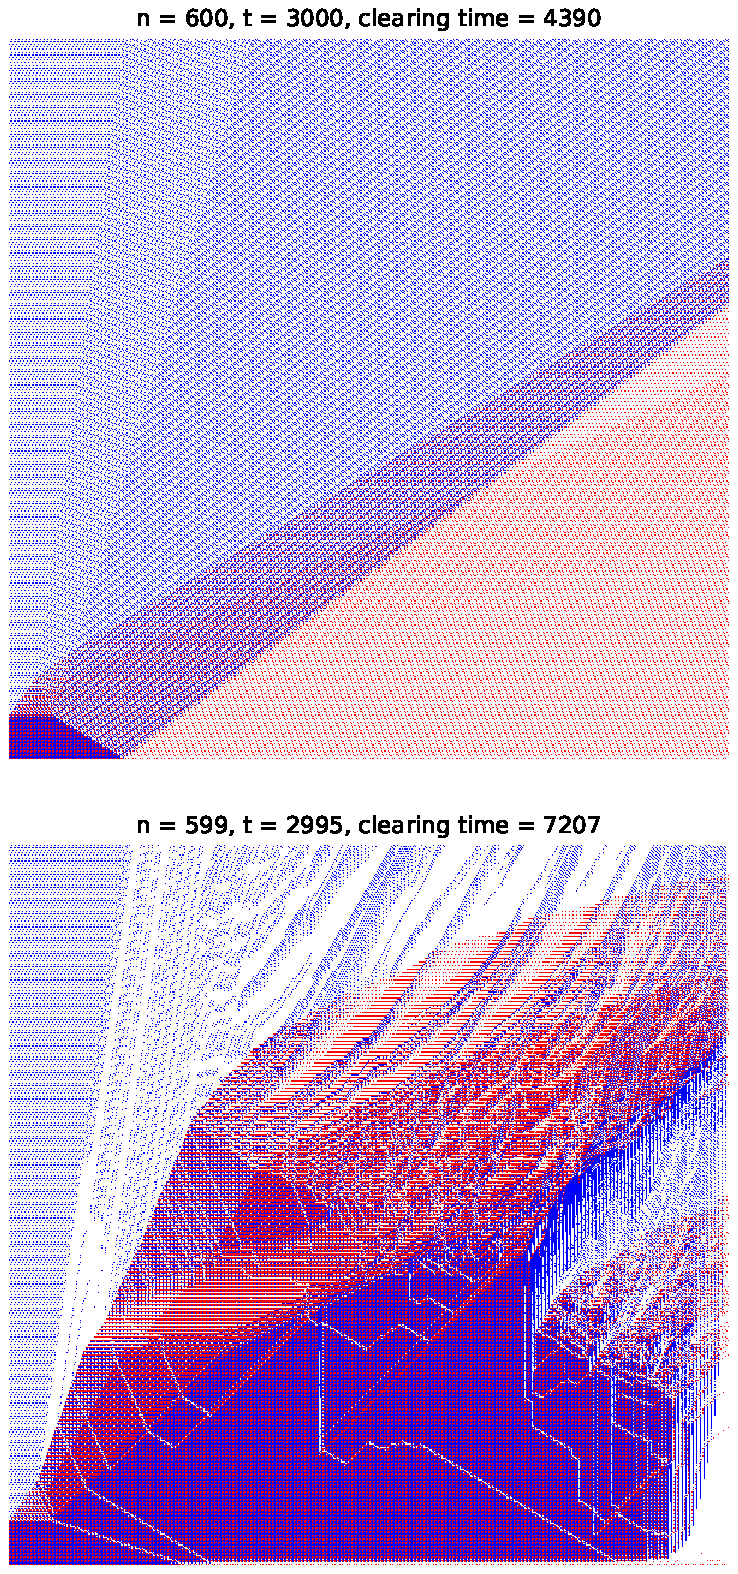
\includegraphics[width=\linewidth,height=.78\textheight,keepaspectratio]{figures/figure01.pdf}
\caption{The BML model at time $t=5n$ for the initial configurations formed by tiling $[n]^2$ with tile \eqref{eq:interesting_tiling}. Deleting the topmost row and rightmost column changes the evolution and increases the clearing time.}
\label{fig:lin_and_non_linear_behaviour}
\end{figure}

\begin{figure}
\centering
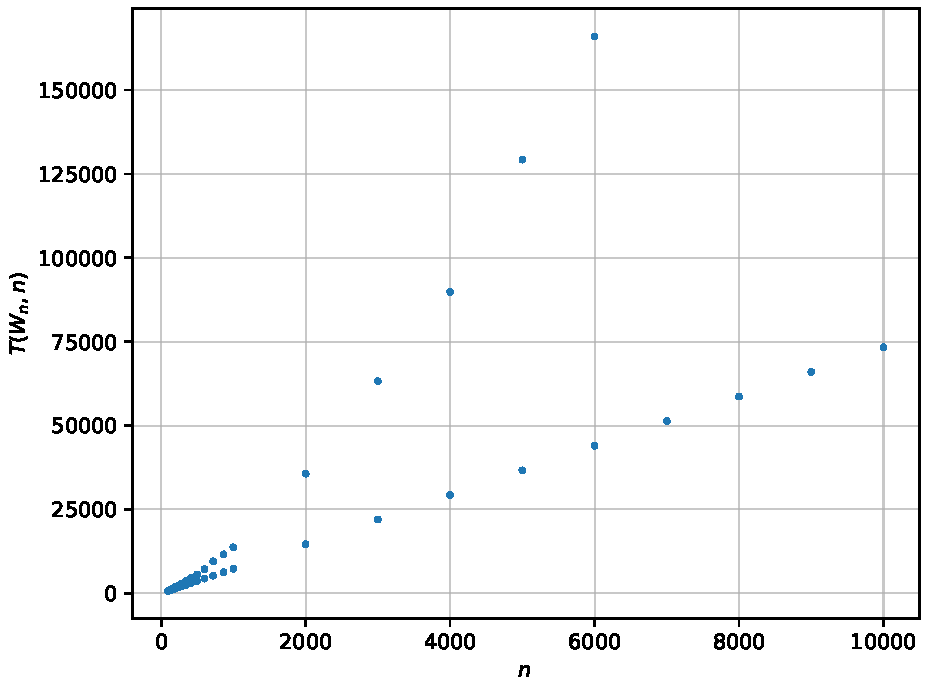
\includegraphics[width=\linewidth,height=.78\textheight,keepaspectratio]{figures/figure02.pdf}
\caption{Clearing times for tile \eqref{eq:interesting_tiling2}. The plot contains \FigureTwoCount{} selected observations up to $n=\FigureTwoMaxN$. The different curves correspond to residue classes modulo $3$.}
\label{fig:graph_subsequences}
\end{figure}

Besides clearing times, we will discuss several striking phenomena in the observed evolution of the superlinear configurations. These include the emergence of \textit{fault-lines} - diagonal boundaries of empty space that separate blocked regions and tend to proliferate with system size; \textit{highways} - narrow corridors of unimpeded flow enabled by localised blocking; and \textit{reorganisation}, in which the system rapidly settles into a different periodic structure with only limited car movement. Each of these behaviours contributes to the complex, nonlinear dynamics observed during clearing. In particular, the number and size of fault-lines and highways appear to grow with the grid size $n$, providing a plausible mechanism for the observed superlinear clearing times in certain configurations. We also compare these behaviours to those in randomly generated initial states, which—though less structured—exhibit similar chaotic patterns and evidence of non-linear scaling. See Section \ref{sec:heuristic} for more discussion.

\subsection*{Implications for the phase transition}

As mentioned earlier, the asymptotic behaviour of $\Tmax$ has bearing on the conjectured phase transition of the model with random initial condition $\mathcal{W}$.  As we explain next, our findings cast potential doubt on the accepted picture, and in fact lend plausibility to the outlandish possibility that the model on $\Z^2$ might jam almost surely for \emph{every} strictly positive value of the parameter $p$.

Here is the heuristic reasoning. Suppose, as our results suggest, that $\Tmax$ grows superlinearly with $n$.  Fix $p$ (small), and consider some large $n$.  Almost surely, the initial configuration $\mathcal{W}$ contains some $n$-by-$n$ square containing a ``worst'' jam, i.e. one that takes $\Tmax$ to clear.  While this jam clears, the square can be expected to accumulate a stationary ``tailback'' of approximately $n p \cdot\Tmax$ new cars which run into it from the South and West (because it presents an obstacle of width $n$, and cars occur with density $p$).  For fixed $p$ and $n$ sufficiently large, we have $n p \cdot \Tmax \gg n^2$.  Therefore, by time $\Tmax$, a new jam has accumulated that is much larger than the original one.  If this new jam similarly takes superlinear time to clear then an even larger one will form, and so on.  Even if such endlessly growing jams are very rare, it is plausible that they will lead to jamming of the entire configuration.

The above argument falls far short of a rigorous proof, for many reasons.  Perhaps most notably, we cannot be sure that tailbacks will behave as ``bad'' jams with large clearing times.  The structure of tailbacks is likely to be very complicated, since they arise from the output of other jams elsewhere in the configuration.  Perhaps some form of self-organization leads them to clear in linear time.  On the other hand, our investigations tend to suggest that superlinear clearing times of finite jams are in some sense typical, as opposed to restricted to special worst cases.

We note that for bootstrap percolation models, an argument somewhat analogous to the one given above can be made rigorous, proving the ostensibly surprising fact that the model is in a certain sense ``supercritical'' for every positive initial density. See \cite{vanenter,schonmann}.

In summary, while there is much uncertainty, we believe that the possibility of jamming for all positive $p$ at least deserves serious consideration.

\subsection*{Simulation methods}
We next discuss some practical details. We start by arguing that for an initial configuration supported on $[n]^2$ cars can be ignored once they leave $[n]^2$. (This is convenient for simulation.)

To justify open-boundary simulations, it is useful to compare them with the
full-lattice dynamics. Put
\[
 \mathcal L=\{(x,y)\in\mathbb Z^2:x\leq0,\ y\leq0\}.
\]
The \textbf{quadrant BML model} has the same updates as the BML model, except
that cars are deleted immediately after leaving $\mathcal L$. As throughout
the paper, the transition from time $t-1$ to time $t$ updates North cars when
$t$ is odd and East cars when $t$ is even.

\begin{proposition}\label{prop:cars_leaving_dont_matter}
For any initial configuration supported on $\mathcal L$, the full-lattice BML
model and the quadrant BML model agree on $\mathcal L$ at every time.
\end{proposition}

\begin{lemma}\label{lem:free_flowing}
In the full-lattice BML model started from a configuration supported on
$\mathcal L$, every North car that leaves $\mathcal L$ subsequently moves on
every North update. Every East car that leaves $\mathcal L$ subsequently
moves on every East update.
\end{lemma}

\begin{proof}
North cars have fixed horizontal coordinates and East cars have fixed
vertical coordinates. Consequently, cars in $\mathcal N$ are North cars
and cars in $\mathcal E$ are East cars, where
\[
 \begin{aligned}
 \mathcal N&=\{(x,y):x\leq0,\ y\geq1\},\\
 \mathcal E&=\{(x,y):x\geq1,\ y\leq0\}.
 \end{aligned}
\]
There are no cars in the remaining exterior quadrant. We prove by induction
over updates that the following conditions hold:
\begin{enumerate}
 \item No two North cars in a column of $\mathcal N$ are adjacent, and no
 two East cars in a row of $\mathcal E$ are adjacent.
 \item For every $x\leq0$, sites $(x,0)$ and $(x,1)$ are not both occupied
 by North cars. For every $y\leq0$, sites $(0,y)$ and $(1,y)$ are not both
 occupied by East cars.
\end{enumerate}
Both conditions hold initially because the exterior is empty. On a North
update, condition~1 ensures that every North car in $\mathcal N$ has an
empty site above it, so all
these cars move and their separation is preserved. Fix a column $x\leq0$.
A North car entering $\mathcal N$ in that column moves from $(x,0)$ to
$(x,1)$. Its destination was empty; any exterior North car in that column
whose $y$-coordinate was at least $2$ now has $y$-coordinate at least $3$.
Thus the entering car is not adjacent to another exterior car.
Moreover, its old site $(x,0)$ cannot simultaneously be filled by
another North car: that site was occupied before the update. The two
conditions are therefore preserved. If no car enters $(x,1)$, that
site is empty after the update, so condition~2 also holds in that case.
An East update does not change the positions of North cars, and the
analogous argument preserves conditions~1 and~2 for East cars.
This proves the induction.
\end{proof}

\begin{proof}[Proof of Proposition~\ref{prop:cars_leaving_dont_matter}]
The two models agree at time $0$. Suppose they agree on $\mathcal L$ at
time $t-1$. If $t$ is odd, the only possible difference between the models
in the positions of North cars within $\mathcal L$ between times $t-1$
and $t$ is whether a car moves from $(x,0)$ to $(x,1)$, with $x\leq0$.
When $(x,0)$ contains a North car at time $t-1$, condition~2 in the
preceding proof ensures that $(x,1)$ contains no North
car; it contains no East car either. The destination is therefore empty
in the full-lattice model, just as in the quadrant model. Both models
remove the car from $\mathcal L$. All remaining North moves depend only
on sites in $\mathcal L$, and the East cars do not move. If $t$ is even,
the same reasoning applies to moves from $(0,y)$ to $(1,y)$. No car can
enter $\mathcal L$ from outside because movement is only North or East.
Thus the models agree at time $t$, completing the induction.
\end{proof}

We now provide a brief explanation of our simulation methodology. The simulations were implemented in Python.  The BML update rule was converted to a vectorised form which allowed us to take advantage of optimisations in NumPy. For more details on this algorithm see Appendix \ref{app:A}. Using this algorithm we see a substantial increase in speed over traditional implementations. This allowed us to simulate select configurations up to $n=10000$ for time steps $t > 10^6$ (corresponding to more than $10^{14}$ site updates) in a reasonable time frame. These large system sizes were crucial in obtaining convincing evidence of some of our findings. The simulation work was carried out using the computational facilities of the Advanced Computing Research Centre, University of Bristol - \url{http://www.bristol.ac.uk/acrc/}. 

\section{Upper Bound for \texorpdfstring{$\Tmax$}{the Maximal Clearing Time}}

In this section we prove the upper bound in Theorem \ref{thm:upper_bound} the time to clear of the model on finite $n$-by-$ n$ grids. This will be done by finding an upper bound for the clearing time of the East cars in the top row of the $n$-by-$ n$ grid. We first introduce a new model with deterministic dynamics on East cars in a $1 $-by-$ n$ grid called the Top Row Model (TRM) and argue that this model captures every possible evolution of the East cars in the top row of the BML model. An explicit upper bound for the clearing time of this Top Row Model can found, and this carries over to the top row of the BML model.

Although, as discussed previously, the BML model lacks monotonicity, the key property of the TRM will be a certain form of monotonicity, see Lemma \ref{lem:partial_ordering}.

The TRM evolves at even times. Its state is an $n$-by-$n$ matrix $M$ with
entries indexed by $i,j\in[n]$. Column $j$ represents a car currently in
position $j$; entry $M(i,j)$, for $i\geq j$, records its waiting time at
the present or future position $i$. A state is \emph{valid} if
\begin{enumerate}
\item $M(i,j)\in\{0,2,4\}$ for all $i,j$;
\item $M(i,j)=0$ when $i<j$;
\item each column $j$ is either identically zero or satisfies
$M(i,j)\in\{2,4\}$ for every $i\geq j$.
\end{enumerate}
We write $\mathcal M$ for the set of valid states, and call each nonzero
column a \emph{stack}. Thus the potentially nonzero entries form the
lower triangle in the usual matrix convention. A stack is \emph{blocked}
if the column immediately to its right is a stack. Column $n+1$ is
regarded as empty, and a stack moving right from column $n$ exits.

Let $\mathcal U(M)$ denote the state two time steps after $M$. Every
stack in column $j$ is updated simultaneously as follows, using the
occupancies in $M$:
\begin{enumerate}
\item If it is blocked, leave it unchanged.
\item If it is unblocked and $M(j,j)=4$, leave it in column $j$ and
replace its diagonal entry by $2$.
\item If it is unblocked and $M(j,j)=2$, move it to column $j+1$,
discarding its old diagonal entry. If $j=n$, remove the stack.
\end{enumerate}
The moved stack in column $j+1$ has entries $M(i,j)$ for $i\geq j+1$,
and zero entries for $i<j+1$. These rules preserve validity. To make the
simultaneous convention explicit, each old stack contributes either
its stationary column or its moved column to the new state; initially
empty columns contribute nothing. A move has an initially empty
destination, so two contributions cannot conflict.

For $j\in[n]$, define $f_j:\mathcal M\to\mathcal M$ by shifting stack
$j$ one position to the right and discarding its diagonal entry when
its destination is empty; otherwise let $f_j(M)=M$. If column $j$ is
empty, this map also leaves $M$ unchanged. More explicitly, for $j<n$
with column $j+1$ empty,
\[
\bigl(f_j(M)\bigr)(i,l)=
\begin{cases}
 M(i,l),&l\notin\{j,j+1\},\\
 0,&l=j,\\
 M(i,j),&l=j+1\text{ and }i\geq j+1,\\
 0,&l=j+1\text{ and }i<j+1.
\end{cases}
\]
The map $f_n$ simply replaces column $n$ by zero. For
$1\leq j\leq i\leq n$, define
\[
\bigl(g_{i,j}(M)\bigr)(k,l)=
\begin{cases}
 2,&(k,l)=(i,j)\text{ and }M(i,j)=4,\\
 M(k,l),&\text{otherwise}.
\end{cases}
\]
In particular, $g_{i,j}$ changes only its specified entry.

We call each individual map $f_j$ or $g_{i,j}$ an \emph{update map}. A single
application shifts one stack or reduces one waiting-time entry when the
map's conditions hold; otherwise it leaves the state unchanged.

Define $M\succeq N$ when $N$ can be obtained from $M$ by a finite
composition of these update maps, including the empty composition
(which gives $M=N$).
This relation is a partial order. Reflexivity and transitivity follow
from its definition. Whenever an update map changes the state, it
strictly decreases
\[
    P(M)=\sum_{i,j}M(i,j):
\]
reducing an entry from $4$ to $2$ decreases the sum by $2$, while shifting
a stack discards a diagonal entry equal to $2$ or $4$. Consequently, a
sequence of update maps that changes the state cannot return to its
starting state. This proves antisymmetry. In particular,
$0\succeq N$ implies $N=0$.

\begin{lemma}\label{lem:partial_ordering}
If $M,N\in\mathcal M$ and $M\succeq N$, then
$\mathcal U(M)\succeq\mathcal U(N)$.
\end{lemma}
\begin{proof}
We first prove the conclusion when $N$ is obtained from $M$ by applying
one update map: either $N=f_j(M)$ or $N=g_{i,j}(M)$.
To see why this is enough, the definition of $M\succeq N$ gives a finite
sequence of valid states
\[
 M=M^{(0)},\ M^{(1)},\ldots,\ M^{(r)}=N,
\]
where each $M^{(a+1)}$ is obtained from $M^{(a)}$ by one of these update maps.
Once the conclusion is proved for every such pair, we can apply it to
each consecutive pair in this sequence to obtain
\[
 \mathcal U(M)=\mathcal U(M^{(0)})
 \succeq\mathcal U(M^{(1)})\succeq\cdots
 \succeq\mathcal U(M^{(r)})=\mathcal U(N).
\]
Transitivity then gives the required conclusion. If no update maps are applied
($r=0$), then $M=N$ and the conclusion is immediate.

We now check the two types of update map. Write
$\widehat M=\mathcal U(M)$ and $\widehat N=\mathcal U(N)$.
The assertion is immediate when the chosen update map leaves $M$ unchanged.

First let $N=g_{i,j}(M)$ with $M(i,j)=4$. If $i>j$, both stacks have
the same diagonal entry and make the same move. If they stay in column
$j$, then $\widehat N=g_{i,j}(\widehat M)$. If they move to column
$j+1$, then $\widehat N=g_{i,j+1}(\widehat M)$. All other stacks make
the same updates in the two states. If $i=j$ and stack $j$ is blocked,
then $\widehat N=g_{j,j}(\widehat M)$. If it is unblocked, the stack in
$M$ waits with its diagonal changed to $2$, whereas the stack in $N$
moves or exits. Therefore $\widehat N=f_j(\widehat M)$.

Now let $N=f_j(M)$ be a nonidentity shift. In $M$, column $j$ contains
a stack and its destination is empty. Only the outcomes of that stack
and the stack originally in column $j-1$, if present, can differ. We
check the four cases given by the occupancies of columns $j-1$ and
$j+2$. The following factorisation records the same cases, including
the two possible diagonal values of each affected stack.

Suppose first that $j<n$, and put
\[
    b=M(j,j),\qquad c=M(j+1,j).
\]
Let $I$ denote the identity map. Define a map $A$ by this table,
where ``occupied'' refers to the initial state $M$:
\[
\begin{array}{c|c|c|c}
\text{column }j+2&b&c&A\\ \hline
\text{occupied}&4&\text{either}&f_j\\
\text{occupied}&2&\text{either}&I\\
\text{empty}&4&4&g_{j+1,j+1}\circ f_j\\
\text{empty}&4&2&f_{j+1}\circ f_j\\
\text{empty}&2&4&g_{j+1,j+1}\\
\text{empty}&2&2&f_{j+1}
\end{array}
\]
For $j=n-1$, column $j+2=n+1$ in this table is empty and $f_{j+1}=f_n$
is the exit map. For $j=n$, instead put
\[
 A=\begin{cases}f_n,&M(n,n)=4,\\ I,&M(n,n)=2.\end{cases}
\]
Finally, set
\[
 H=\begin{cases}
 I,&j=1\text{ or column }j-1\text{ is empty},\\
 g_{j-1,j-1},&M(j-1,j-1)=4,\\
 f_{j-1},&M(j-1,j-1)=2.
 \end{cases}
\]
The required identity in every case is
\begin{equation}\label{eq:TRM-shift-cases}
    \widehat N=(H\circ A)(\widehat M).
\end{equation}

To verify \eqref{eq:TRM-shift-cases}, first consider the stack originally
in column $j$. If $j<n$ and column $j+2$ is occupied, the shifted stack
in $N$ is blocked in column $j+1$. In $M$, it either waits in column
$j$ when $b=4$, or moves to column $j+1$ when $b=2$. If $j<n$ and
column $j+2$ is empty, the shifted stack in $N$ either waits with its
new diagonal reduced from $4$ to $2$ when $c=4$, or moves again or exits
when $c=2$. For $j=n$, $A$ removes the waiting stack from $\widehat M$
if $M(n,n)=4$, while for $M(n,n)=2$ it has already exited. In each case,
applying $A$ to $\widehat M$ gives the same outcome for this stack as in
$\widehat N$ and leaves column $j$ empty. If $j>1$ and there was a stack in column $j-1$,
that stack was blocked in $M$, but is unblocked in $N$.
It therefore either reduces its diagonal from $4$ to $2$, or moves
into the now empty column $j$. These are exactly the two nonidentity
choices of $H$. If there is no such stack, $H=I$. All other stacks
have identical updates, proving \eqref{eq:TRM-shift-cases}. Both $A$
and $H$ are compositions of the update maps defined above,
with the identity represented by an empty composition. Thus
$\widehat N$ can be obtained from $\widehat M$ by a finite sequence of
these update maps, so $\widehat M\succeq\widehat N$ by definition.
\end{proof}

Let $M^*$ be the valid state whose entries on and below the diagonal
are all $4$. This is the greatest element under $\succeq$.

For $M\in\mathcal M$, let
\[
 T_M=\inf\{t\in2\mathbb Z_{\geq0}:M_0=M,\ M_t=0\},
\]
with the convention $\inf\varnothing=\infty$. In particular, $T_0=0$.

\begin{lemma}\label{lem:maximal_time}
The all-$4$ state satisfies $T_{M^*}=8n-4$.
\end{lemma}

We first record the corresponding one-dimensional BML calculation.
\begin{lemma}\label{lem:bml_top_row}
The BML model on $[n]\times\{0\}$, initially filled with East cars,
clears in $4n-2$ time steps.
\end{lemma}
\begin{proof}
Label the cars from right to left by $q=1,\ldots,n$ and number East
updates by $1,2,\ldots$. Car $q$ first moves on East update $q$ and then
moves on every East update until it exits. This follows by induction:
after the preceding car first moves, it continues to move and leaves
one empty site between itself and its follower. Car $q$ must make $q$
moves to exit, so its exit update is $2q-1$. The last car exits at
time $2(2n-1)=4n-2$.
\end{proof}

\begin{proof}[Proof of Lemma~\ref{lem:maximal_time}]
At each time $4r$, every nonzero entry of the all-$4$ evolution is $4$.
During the update to time $4r+2$, unblocked stacks reduce their diagonals
to $2$, and no stack changes position. During the update to time
$4r+4$, precisely those stacks move, and their new diagonals, if any,
are again $4$. Blocked stacks remain unchanged. Thus, on the times
$0,4,8,\ldots$, the stack positions follow exactly the one-directional
car evolution in Lemma~\ref{lem:bml_top_row}, with one East update per
four time steps instead of two. The last exit occurs after $2n-1$
such updates, giving $T_{M^*}=4(2n-1)=8n-4$.
\end{proof}

\begin{lemma}\label{lem:TRM_bound}
If $M\succeq N$, then $T_M\geq T_N$. Moreover,
\[
    \max_{M\in\mathcal M}T_M=8n-4.
\]
\end{lemma}
\begin{proof}
Lemma~\ref{lem:partial_ordering} preserves the order at every even time.
Since $0\succeq N$ implies $N=0$, the state started from $N$ is empty
whenever the state started from $M$ is empty. Hence $T_N\leq T_M$.
Every state is below $M^*$, whose clearing time is $8n-4$ by
Lemma~\ref{lem:maximal_time}; this also proves finiteness of every
$T_M$. The all-$4$ state attains the bound.
\end{proof}

\begin{proof} [Proof of Theorem \ref{thm:upper_bound}]
    First notice an East car in column $j$ of the top row of the BML model can be blocked at most once by North cars before it moves to column $j+1$ (because car movements are restricted to odd and even time steps). At any even time at which an East car is not blocked by another East car to its right it will move in $2$ or $4$ time steps. Therefore, there exists some initial state for the TRM such that the resulting movements of stacks exactly mimics the movements of East cars in the top row of the BML model. Hence, by Lemma \ref{lem:TRM_bound} the top row of the BML model is cleared of East cars by time $8n-4$. By a similiar argument, the BML model is cleared of North cars in the rightmost column by time $8n-3$. At time $8n-4$, we are left with a configuration of the BML model on an $n-1 $-by-$ n-1$ grid with only unblocked North cars above it and unblocked East cars to its right. Hence, by Proposition \ref{prop:cars_leaving_dont_matter}, from time $t=8n-4$, the model evolves from a configuration supported on $ [n-1]^2$. The East cars in the second row leave before time $(8n-4) + (8(n-1)-4)+2$. (Notice $2$ is added to this time since once cleared of the $n-1 $-by-$ n-1$ grid, they still have to leave from column $n$ but since all columns to the right are clear of North cars it is freely moving so moves every $2$ time steps). Iteratively applying this argument we see that the East cars in the unlocked $[k-1]^2$ grid leave in $8k-4 + 2(n-k)$ time steps. Hence, summing each of these times gives us,
    $\Tmax \leq \sum_{k=1}^n (8k-4) + 2(n-k)) = 5n^2-n$.
\end{proof}

\section{Periodic Configurations}
In this section we consider the periodic configurations which serve as our primary examples of configuration sequences with superlinear clearing times. Fix $k \in \Z$, and fix a $k$-by-$k$ tile of cars and empty spaces (an element of $\{ \uparrow, \rightarrow,0 \}^{[k]^2}$. We call the configuration $W$ formed by tessellating $\Z^2$ from a tile at the origin a $k$-\textbf{periodic} configuration. Let $(W_n)_{n \geq 1}$ be the restriction of $W$ to $[n]^2$.

We performed simulations of all sequences $(W_{nk})$ for $k \in \{2,3\}$ with no empty spaces. We further perform simulations of the sequences $(W_{nk+i})$ for $k = 3$ and $i \in \{0,1,2\}$ for a select few configurations. In each of these cases it appears that it is easy to separate between linear and superlinear. Furthermore, in each of the linear cases we provide a conjectured linear term for the affine function and in each of the superlinear cases we provide a conjectured power law growth rate with the specified power. For more details, see Appendix \ref{app:A}. In the remainder of this section we deal with some representative examples from the exhaustive analysis.

In the linear cases the clearing times are equal to an affine function plus a periodic function. Furthermore, it seems there is a way to explicitly describe the space-time evolution of the linear periodic sequences. In each case of these sequences, we believe that it is straightforward to prove the space-time evolution and their respective clearing time, albeit laborious. We provide a non-trivial example of this in the $2$-periodic case. In general these evolutions become laborious to explicitly describe but in principle all linear configurations seem to have this property. In the superlinear case, the clearing times seem to grow like a non-trivial power of $n$.

\subsection{Linear configurations} \label{sec:linearconfigs}
Here we address space time evolution of the linear configurations focusing on a few illustrative examples.
We begin with the trivial periodic configuration in which the $k $-by-$ k$ tile is filled with one type of car. In this case there is a simple formula for its clearing time and this provides a lower bound $\Tmax$ which depends linearly on $n$.

\begin{proposition} \label{prop:linear_filled}
    Let $(W_n)_{n \geq 1}$ be the configuration sequence formed from the configuration $W(x)=\ra$ for all $x \in \Z^2$. Then $$T(W_n,n) = 4n-2.$$
\end{proposition}

\begin{proof}
    This follows from Lemma \ref{lem:bml_top_row}.
\end{proof}

We next discuss a particular a $2 $-by-$ 2$ periodic configuration for which we will explicitly describe the space-time evolution.  We further demonstrate a description of the space-time evolution which could be used to show that this configuration sequence is linear. The case checking needed to prove this space-time evolution is laborious even for this simple case, and likely proves to be infeasabile in general.

\begin{theorem}\label{thm:alternating-columns}
Let $W_n$ be the restriction to $[n]^2$ of the periodic configuration with tile
\begin{equation}\label{eq:lineartiling}
    \begin{split}
    \begin{tikzpicture}[scale=1.1]
        \rc{0}{0} \uc{0.6}{0}
        \rc{0}{-0.6} \uc{0.6}{-0.6}
    \end{tikzpicture}.
    \end{split}
\end{equation}
Thus every odd-numbered column contains East cars and every even-numbered
column contains North cars initially, with columns numbered from the left.
For every integer $n\geq1$,
the complete evolution is the function $F_n$ below, whose pieces agree with
periodic patterns on regions bounded by affine inequalities. In particular,
$T(W_n,n)=6n-4$.

Use Cartesian coordinates $(x,y)\in[n]^2$, with $x$ increasing from left
to right and $y$ from bottom to top, so that $(1,1)$ is the bottom-left
site. For integer $t\geq0$, put
\[
 q=\left\lfloor\frac{t-1}{2}\right\rfloor,
 \qquad r=\left\lfloor\frac t2\right\rfloor,
 \qquad b=r-2n+3.
\]
Define $F_n(x,y,t)$ by the following rules.
\begin{enumerate}
\item If $y\geq b$ and $4y+t\leq4n-2$, set $F_n(x,y,t)=\ra$ when
$x$ is odd and $F_n(x,y,t)=\ua$ when $x$ is even.
\item If $y\geq b$ and $4y+t\geq4n-1$, set $F_n(x,y,t)=\ua$ when
$x$ is even and $y\equiv n+q+1\pmod3$. Otherwise set $F_n(x,y,t)=\ra$
when
\[
 3x-4y\geq t-4n+1
\]
and either $x$ is even with $y\equiv n+r-1\pmod3$, or $x$ is odd with
$y\not\equiv n+r-1\pmod3$.
\item If $y<b$, set $F_n(x,y,t)=\ra$ when
\[
 x-y>r-2n+1,\qquad x-y-r\equiv0\pmod2.
\]
\end{enumerate}
All remaining sites are empty. For odd $n$, impose the additional boundary
rule
\begin{equation}\label{eq:alternating-boundary}
 F_n(n,y,t)=0\quad\text{if}\quad
 r\geq1,\quad y\geq b,\quad
 \bigl(r<2n-2y+1\ \text{or}\ y\equiv n+r\pmod3\bigr).
\end{equation}
This rule takes precedence over the East-car assignments above.
After fixing the parity of $t$, all the inequalities defining the pieces
are affine in $x,y,t,n$; within each piece, the state is determined by
the displayed congruences, giving a restriction of a pattern with periods
$2$, $6$ and $12$ in $x$, $y$ and $t$, respectively.
Thus the rules describe the periodic patterns
and their moving boundaries throughout the evolution, for both parities
of $n$.
\end{theorem}

\begin{proof}
In these coordinates, a North move increases $y$ and an East move increases $x$.
Call the North update at time $2r-1$ and the East update at time $2r$
\emph{cycle $r$}. For $n=1$, the displayed rules give a single East car at
times $0$ and $1$, and the empty state thereafter, as required.
Assume henceforth that $n\geq2$.

We verify the stated function by tracking individual cars. Put
\[
    S_y=2n-2y+1,\qquad C_y=2n+y-2,\qquad a_y=y-1,
\]
and, for integers $r\geq0$, define
\begin{equation}\label{eq:alternating-displacement}
d_y(r)=
\begin{cases}
0, & 0\leq r<S_y,\\[2pt]
\displaystyle\left\lceil\frac{2(r-S_y+1)}{3}\right\rceil,
    & S_y\leq r<C_y,\\[6pt]
r-2n+y+1, & r\geq C_y.
\end{cases}
\end{equation}
Notice that $C_y=S_y+3a_y$. Equivalently, the increments of $d_y$ are
zero before cycle $S_y$; they are $1,1,0$ on the successive triples
\[
    S_y+3h,\quad S_y+3h+1,\quad S_y+3h+2,
    \qquad 0\leq h<a_y;
\]
and they are $1$ on every cycle from $C_y$ onward.

We claim the following descriptions hold simultaneously.
\begin{enumerate}
\item A North car initially in row $\ell$ first moves on cycle $S_\ell$
and then moves on every North update until it exits. Its row after the
North update of cycle $r$ is
\begin{equation}\label{eq:alternating-north-position}
    \ell+\max\{0,r-S_\ell+1\},
\end{equation}
as long as this number is at most $n$. In particular, it exits on cycle
$3n-3\ell+1$, at time $6n-6\ell+1$.
\item An East car initially in row $y$ and odd column $p$ has column
$p+d_y(r)$ after cycle $r$, as long as it has not exited. An East car
at column $n$ leaves at the next East update, including when the common
displacement is unchanged. More explicitly, its exit cycle is
\begin{equation}\label{eq:alternating-east-exit}
    1+\min\{r\geq0:p+d_y(r)\geq n\}.
\end{equation}
\end{enumerate}
These formulas also specify the intermediate odd times: North cars have
their cycle-$r$ positions at time $2r-1$, whereas East cars still have
their cycle-$(r-1)$ positions.

Here is a simultaneous induction on the cycles verifying both claims.
They give the required initial configuration at cycle $0$. Suppose they
hold through cycle $r-1$.

First consider a North car initially in row $\ell<n$ before its proposed
first move. Until and including cycle $S_{\ell+1}=2n-2\ell-1$, its destination
is occupied before the North update by the North car initially just above
it. That preceding car moves on cycle $S_{\ell+1}$. The East update of
the same cycle moves the surviving East cars in row $\ell+1$ from odd
to even columns, filling every even column of that row. In particular,
on cycle $2n-2\ell$
the North car is again blocked. The subsequent East update moves those
East cars to odd columns or out of the grid, freeing its destination
for cycle $S_\ell$.
The North car in the top row exits immediately on cycle $S_n=1$.

For a proposed move of the car initially in row $\ell$ into row $k\leq n$,
the proposed North-update cycle is
\[
    r=2n+k-3\ell,\qquad \ell<k\leq n.
\]
The preceding car in the same column, if it has not exited, is three
rows ahead before this update, by \eqref{eq:alternating-north-position}.
Thus the destination contains no North car. Write $h=k-\ell-1$.
Then $0\leq h<a_k$ and
\[
    r-1=S_k+3h+1,\qquad d_k(r-1)=2h+2.
\]
Consequently all East cars still in row $k$ occupy odd columns before
this North update, and cannot block the move in an even column. This
verifies every proposed North move; a move out of the top row has an
empty destination outside the grid. It also verifies that no earlier
first move is possible. The first claim therefore holds on cycle $r$.

We next check the East update. All surviving East cars in a row have
the same displacement before the update, so their column indices differ
by at least two. They cannot block one another. Before cycle $S_y$, the
original North car in row $y$ still occupies every even column, and an
East car not at the right boundary cannot move. For $0\leq h<a_y$:
\begin{itemize}
\item On cycle $S_y+3h$, the North car initially in row $y-h$ has just
left row $y$. No following North car can enter that row in the same
update. Its even columns are therefore empty, and the East cars move
from odd to even columns.
\item On cycle $S_y+3h+1$, those East cars move from even to odd columns;
there are no North cars in odd columns.
\item On cycle $S_y+3h+2$, the North car initially in row $y-h-1$ has
just entered row $y$, occupying its even columns. The East cars in odd
columns are blocked, except that a car already at column $n$ exits.
\end{itemize}
On cycle $C_y$, the North car initially in the bottom row leaves row
$y$; no North car subsequently returns to that row. The remaining East
cars therefore move at every East update from cycle $C_y$ onward.
This is exactly the increment schedule in
\eqref{eq:alternating-displacement}. Removing a boundary car does not
affect this argument: it creates no additional East blocker, and when
an interior move is blocked its target contains a North car rather
than an East car. This proves the second claim and completes the
simultaneous induction.

We now recover the regional formula for $F_n$ from these trajectories.
Write $s=\lfloor(t+1)/2\rfloor=q+1$. At time $t$, a site $(x,y)$
contains a North car precisely when $x$ is even and either
\[
 s\leq2n-2y,
\]
or
\[
 2n-2y+3\leq s\leq2n+y-3,\qquad y\equiv n+s\pmod3.
\]
The first case is the North car initially in row $y$, before its first
move. In the second case its initial row is $(2n+y-s)/3$, by
\eqref{eq:alternating-north-position}. These are exactly the North-car
assignments in the first two regions above.

For $x<n$, the site contains an East car precisely when
\[
 x>d_y(r),\qquad x-d_y(r)\equiv1\pmod2.
\]
Indeed, $x-d_y(r)$ is its initial column, which must be positive and odd.
When $r<C_y$, substitution of the middle or initial part of
\eqref{eq:alternating-displacement}, with the three possible values of
$r-S_y$ modulo $3$, gives the East-car assignments in the first two
regions. When $r\geq C_y$, substitution gives
\[
 x>r-2n+y+1,\qquad x-y-r\equiv0\pmod2,
\]
which is the third region, since $r\geq C_y$ is equivalent to $y<b$.
At $x=n$, the same test applies only if $r=0$ or
$d_y(r)>d_y(r-1)$: a car that has already reached the boundary leaves on
the next East update, even when the interior cars wait. The unchanged
displacement occurs exactly when $r<S_y$, or when $S_y\leq r<C_y$ and
$y\equiv n+r\pmod3$. In both cases $d_y(r)$ is even, so the possible
boundary car has odd initial column only when $n$ is odd. This gives
exactly \eqref{eq:alternating-boundary}. Hence the stated $F_n$ agrees
with the evolution at every site and time.

It remains to determine the last exit. All North cars have left by
time $6n-5$. At cycle $r_*=3n-2$, we have $r_*\geq C_y$ for every row
and
\[
    d_y(r_*)=n+y-1\geq n.
\]
No East car can remain, since even the car initially at column $1$
would then have column index greater than $n$. Conversely, in the
bottom row $y=1$, $C_1=2n-1$ and
\[
    d_1(r_*-1)=n-1.
\]
Thus its leftmost initial East car has just reached column $n$ after
cycle $r_*-1$; it remains there through the next North update and exits
on the East update of cycle $r_*$. The clearing time is therefore
$2r_*=6n-4$.
\end{proof}

Figure~\ref{fig:F_n} illustrates the periodic regions and their affine
boundaries in $F_n$.
\begin{figure}
\centering
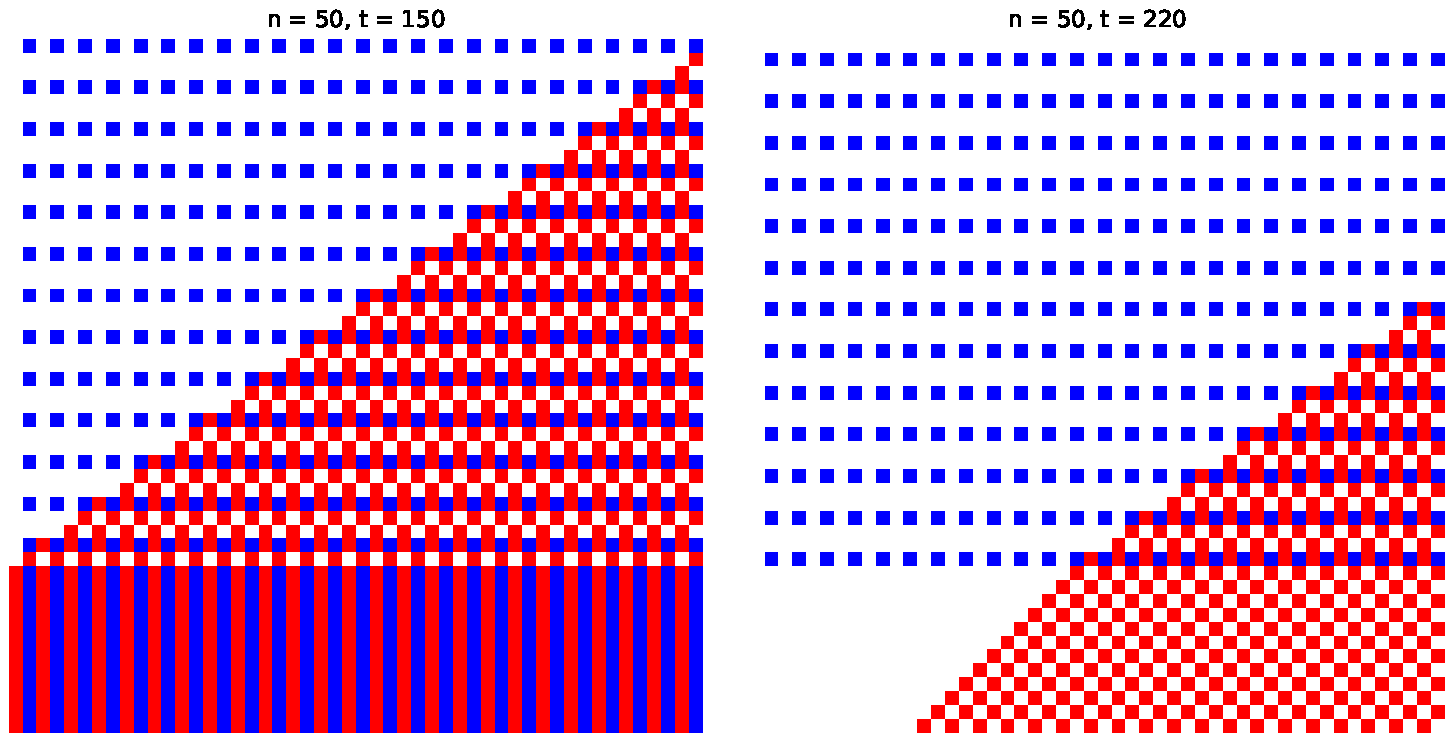
\includegraphics[width=\linewidth,height=.78\textheight,keepaspectratio]{figures/figure03.pdf}
\caption{The explicit evolution $F_{50}$ at times $t=150$ (left) and
$t=220$ (right), with the column phase in \eqref{eq:lineartiling}.}
\label{fig:F_n}
\end{figure}

In principle every conjectured linear configuration sequence from the simulations could be shown to behave in a similiarly explicit way. Observations of the clearing of the conjectured linear periodic configurations show that each time step could in principle be described by a piece-wise function on periodic regions separated by linear boundaries. This would analytically describe the entire evolution of the $n $-by-$ n$ grid. Unfortunately for large periodic configurations, there are many different regions and it becomes difficult to concisely write down descriptions of the evolution. An example of such a configuration is shown in Figure \ref{fig:lots_of_regions}. All $2$-periodic configurations exhibit these periodic regions in clearing and we conjecture that all $2$-periodic configurations clear in linear time.

\begin{figure}
\centering
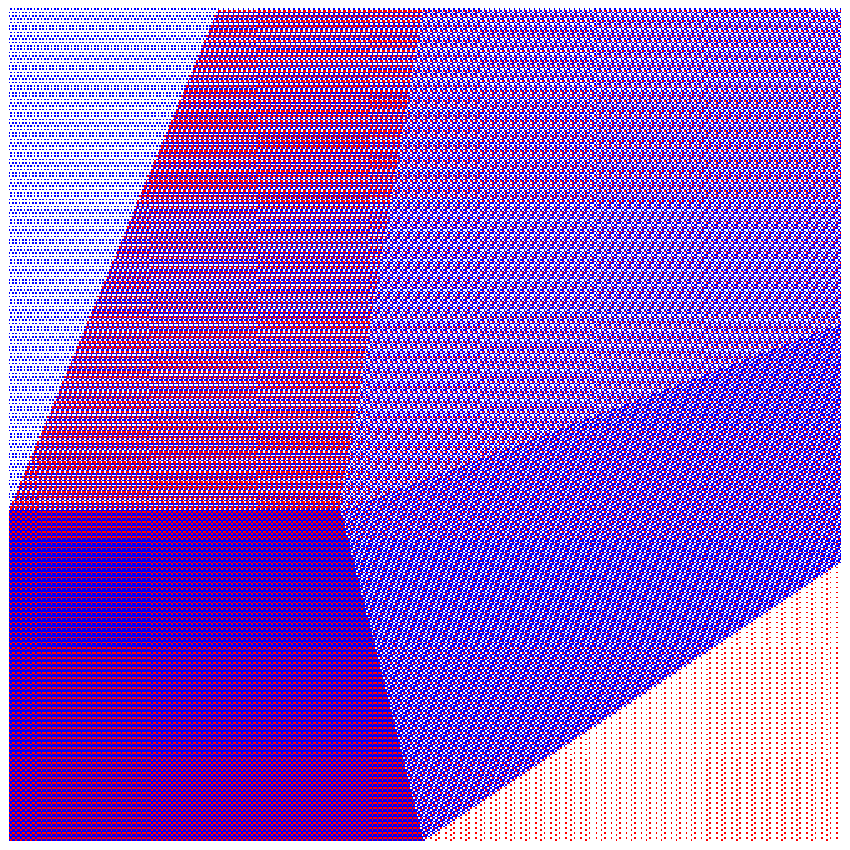
\includegraphics[width=\linewidth,height=.78\textheight,keepaspectratio]{figures/figure04.pdf}
\caption{Evolution of tile $333131313$ at $n=498$ and $t=996$, exhibiting periodic regions separated by affine boundaries.}
\label{fig:lots_of_regions}
\end{figure}
\subsection{Candidate superlinear configurations}
Some periodic initial states develop spatial patterns that appear less
regular than the preceding examples. We use ``irregular'' descriptively,
without asserting a formal property of dynamical chaos. Figure~\ref{fig:periodic_chaos}
illustrates such clearing from a periodic initial configuration.
\begin{figure}
\centering
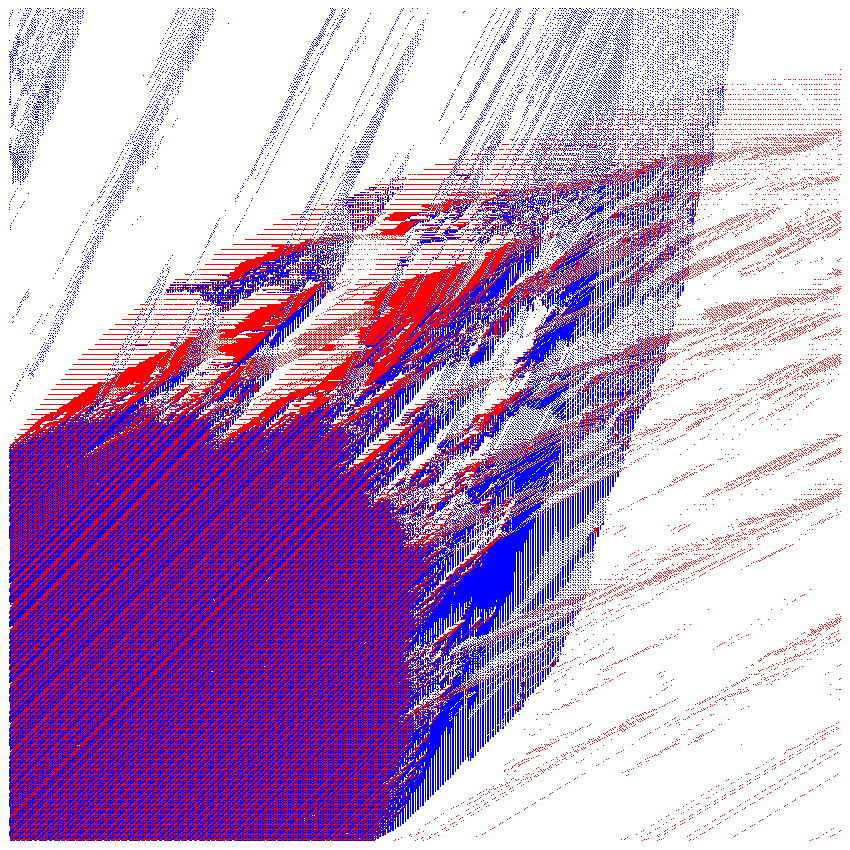
\includegraphics[width=\linewidth,height=.78\textheight,keepaspectratio]{figures/figure05.pdf}
\caption{Evolution of tile \eqref{eq:reorganisation} at $n=999$ and $t=6000$, illustrating aperiodic clearing.}
\label{fig:periodic_chaos}
\end{figure}

All configurations that exhibit this non piece-wise periodic clearing seem to have clearing times which grow like a superlinear function. The chaotic region of clearing appears to form new jams that were not already present in the initial configuration and thus as $n$ increases the number of jams seem to increase superlinearly in $n$. This could explain the asymptotically superlinear clearing time of these configurations. In Section \ref{sec:heuristic} we give specific examples of structures in the superlinear configuration sequences which appear to create extra jams.

An exploratory survey of $3$-periodic configurations identified candidates with large estimated powers in their clearing times. The original survey estimates are retained separately in Appendix~\ref{app:A}. The selected case was the periodic configuration with tiling

\begin{equation} \label{eq:worst3periodic}
\begin{split}
        \begin{tikzpicture}[scale=1.1]
        \rc{0}{0} \rc{0.6}{0} \uc{1.2}{0}
        \rc{0}{-0.6} \uc{0.6}{-0.6} \uc{1.2}{-0.6}
        \uc{0}{-1.2} \rc{0.6}{-1.2} \uc{1.2}{-1.2}
    \end{tikzpicture}
    \end{split}
\end{equation}
We simulated this configuration at \FigureSixCount{} grid sizes from
$n=3$ to $n=\FigureSixMaxN$; the clearing times are shown in
Figure~\ref{fig:clearing_times}.
\begin{figure}
\centering
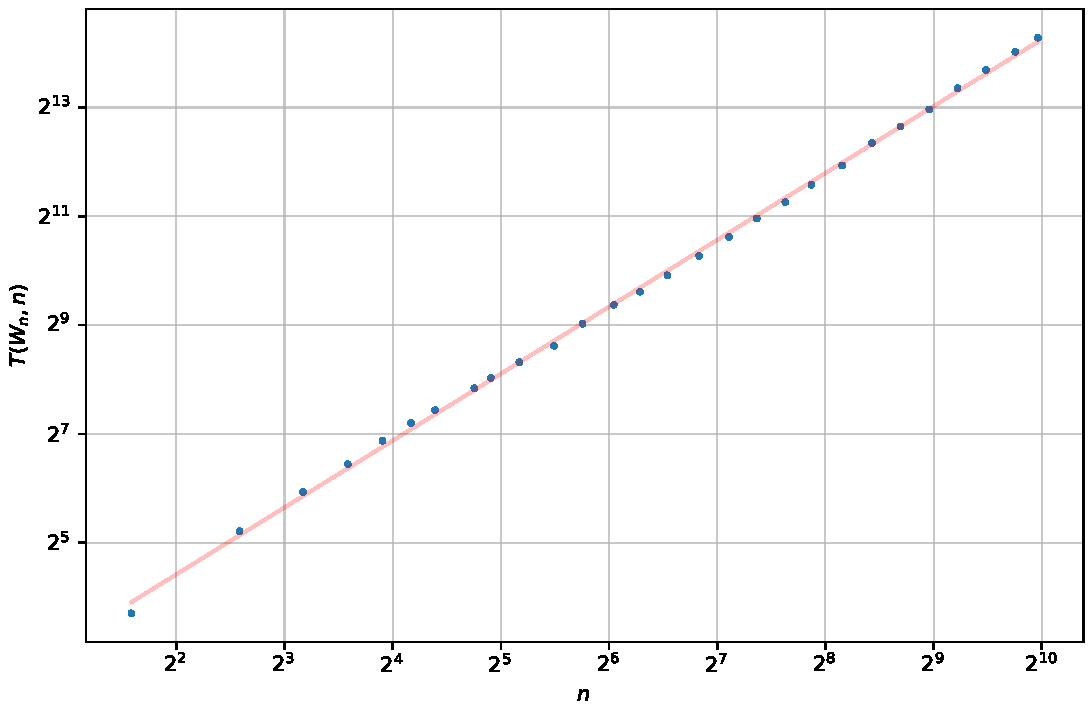
\includegraphics[width=\linewidth,height=.78\textheight,keepaspectratio]{figures/figure06.pdf}
\caption{Log-log clearing times for tile \eqref{eq:worst3periodic}, using \FigureSixCount{} observations up to $n=\FigureSixMaxN$. Least-squares fit: $\log_2 T(W_n,n)=\FigureSixPower\log_2 n+\FigureSixIntercept$.}
\label{fig:clearing_times}
\end{figure}
\subsection{Dependence on \texorpdfstring{$n\bmod3$}{n mod 3}}\label{sec:analytical}
Restricting the same periodic configuration to different grid sizes can
change the observed clearing time substantially. We examine one explicit
example and formulate conjectures depending on $n\bmod3$.

One of the most striking examples of this behaviour is observed in the periodic configuration with tiling 
\begin{equation}\label{eq:interesting_tiling2}  
\begin{split}
        \begin{tikzpicture}[scale=1.1]
        \rc{0}{0} \uc{0.6}{0} \uc{1.2}{0}
        \uc{0}{-0.6} \uc{0.6}{-0.6} \uc{1.2}{-0.6}
        \rc{0}{-1.2} \rc{0.6}{-1.2} \uc{1.2}{-1.2}
    \end{tikzpicture}
    \end{split}
\end{equation}
The sampled clearing times show a strong dependence on $n\bmod3$.
For $n\equiv2\pmod3$, the retained observations have fitted slope
$\FigureSevenSuperlinearPower$ on logarithmic coordinates. For the other
values of $n\bmod3$, the supplied measurements satisfy the exact observed
relations
\[
T(W_n,n)=
\begin{cases}
(22n-30)/3,& n\equiv0\pmod3,\\
(22n-28)/3,& n\equiv1\pmod3,\ n\ge4.
\end{cases}
\]
We conjecture that the displayed affine formulas hold at every size
satisfying their stated conditions.

The figures suggest superlinear growth when $n\bmod3=2$ and linear bounds
otherwise. The asymptotic distinction remains conjectural.
A finite comparison already shows the sensitivity to deletion:
the supplied $n=600$ and $n=599$ configurations have clearing times $4390$
and $7207$, respectively.
\begin{figure}
\centering
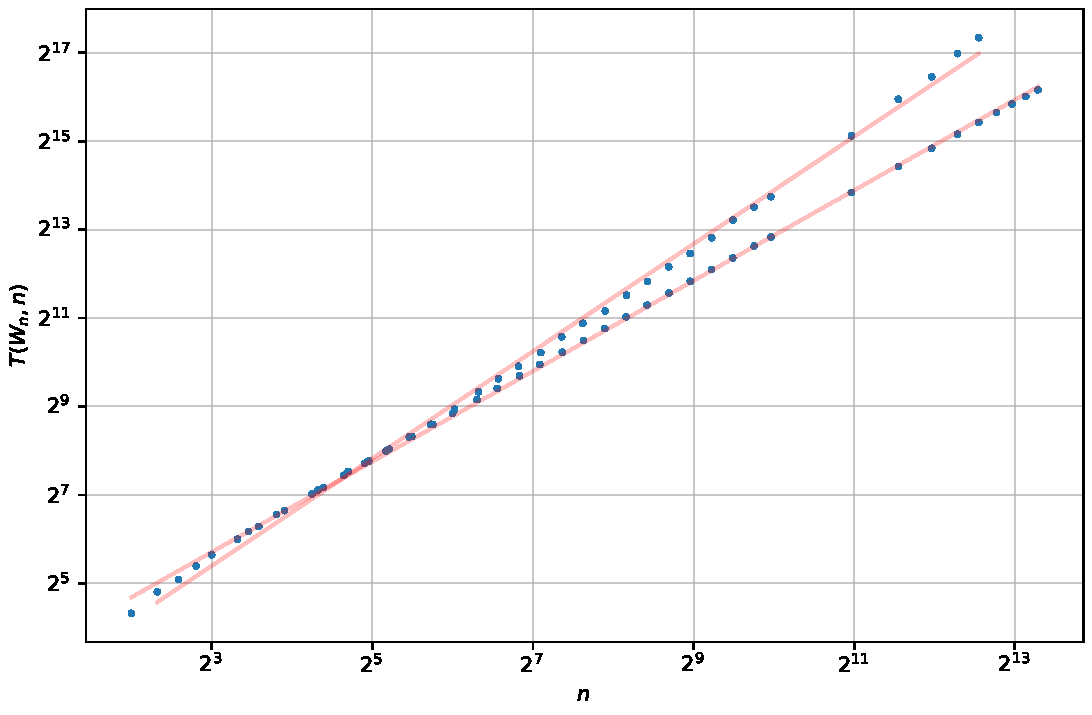
\includegraphics[width=\linewidth,height=.78\textheight,keepaspectratio]{figures/figure07.pdf}
\caption{Clearing times for tile \eqref{eq:interesting_tiling2}, using \FigureSevenCount{} observations up to $n=\FigureSevenMaxN$. The fitted lines are $\log_2 T=\FigureSevenSuperlinearPower\log_2 n+\FigureSevenSuperlinearIntercept$ for $n\equiv2\pmod3$, and $\log_2 T=\FigureSevenOtherPower\log_2 n+\FigureSevenOtherIntercept$ otherwise.}
\label{fig:log_log_graph_subsequences}
\end{figure}
\section{Heuristic Analysis} \label{sec:heuristic}
Here we give a brief overview of the self organising phenomona arising in this model for specific periodic configurations. In particular we give situations in which the number of jams  appears to increase more than linearly with $n$. Ideally, one would be able to construct an initial configuration which forces this behaviour in an analysable way but this has proven to be incredibly difficult.
\subsection{Fault-lines}
We call a diagonal corridor of mostly vacant sites separating blocked
regions a \emph{fault-line}. An example occurs in the configuration with tile
\begin{equation} \label{eq:faultlines}
\begin{split}
    \begin{tikzpicture}[scale=1.1]
        \rc{0}{0} \rc{0.6}{0} \rc{1.2}{0} \rc{1.8}{0}
        \rc{0}{-0.6} \rc{0.6}{-0.6} \rc{1.2}{-0.6} \uc{1.8}{-0.6}
        \rc{0}{-1.2} \rc{0.6}{-1.2} \uc{1.2}{-1.2} \uc{1.8}{-1.2}
        \rc{0}{-1.8} \uc{0.6}{-1.8} \uc{1.2}{-1.8} \uc{1.8}{-1.8}
    \end{tikzpicture}
    \end{split}
\end{equation}
as shown in Figure \ref{fig:fault_lines}.
\begin{figure}
\centering
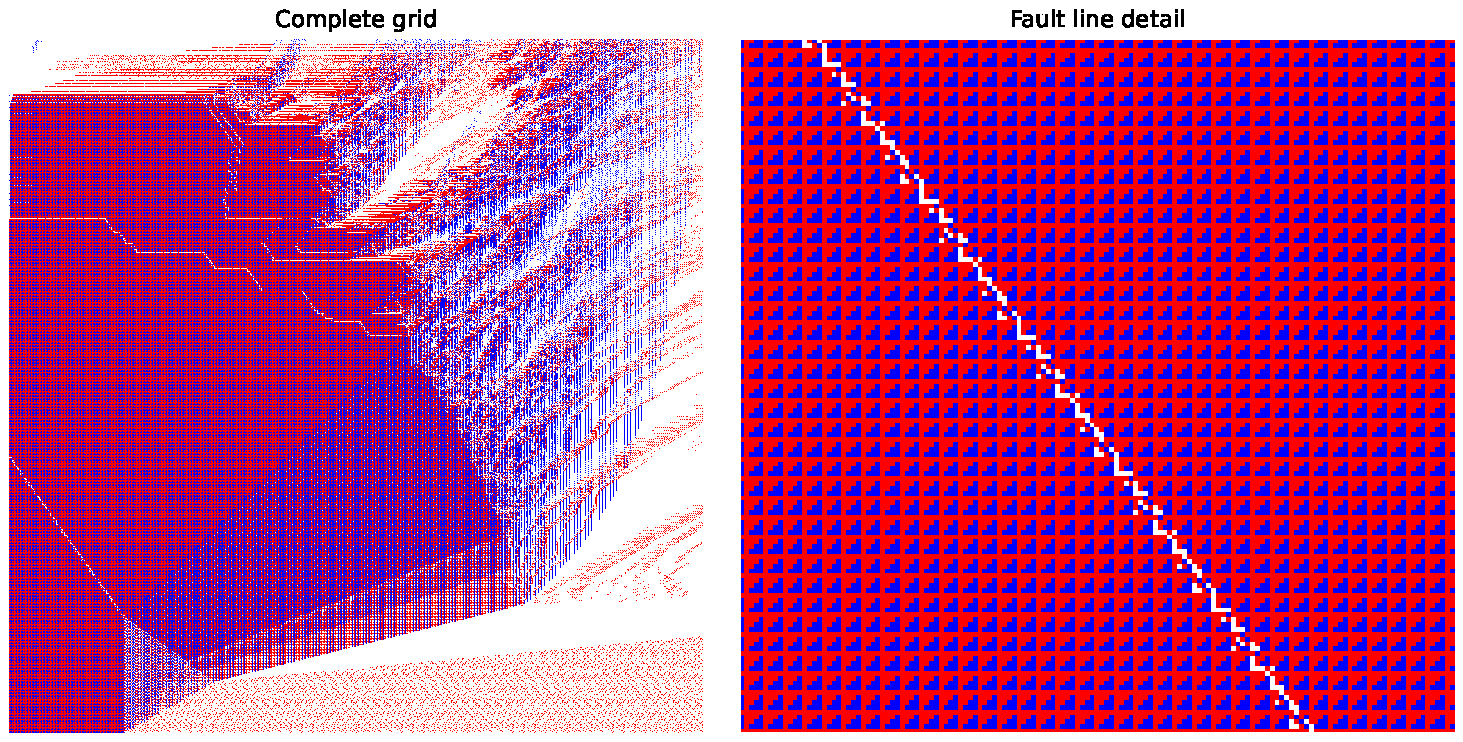
\includegraphics[width=\linewidth,height=.78\textheight,keepaspectratio]{figures/figure08.pdf}
\caption{Evolution of tile \eqref{eq:faultlines} at $n=1000$, $t=5000$. Left: the full grid. Right: the fault-line detail selected by the figure recipe.}
\label{fig:fault_lines}
\end{figure}
Moreover, as $n$ increases the number of fault-lines increase. This becomes extremely noticeable for $n \geq 5000$ (images of which have not been included due to resolution limitations). A fault-line forms when the initial periodic configuration shifts up (or right) by one row (or column). As a result when a car moves for the first time it immediately gets blocked in another large blocked region. The size of these blocked regions increase linearly with $n$ and since the number of fault lines increases with $n$ this could explain the superlinear behaviour of the clearing time for these configurations. This behaviour is common in the periodic configurations.
\subsection{Highways}
A highway forms in a similar way to a fault-line.  In observation of the clearing, a highway can be recognised as a horizontal (or vertical) width $1$ line of mostly empty space with a line of East (or North) cars below it (or to the left of it). The line of East (or North) cars serve to block any cars which could disrupt cars in the mostly empty line. Therefore, cars in this line move at maximal velocity through the blocked region. This can be seen in Figure \ref{fig:highway}.
\begin{figure}
\centering
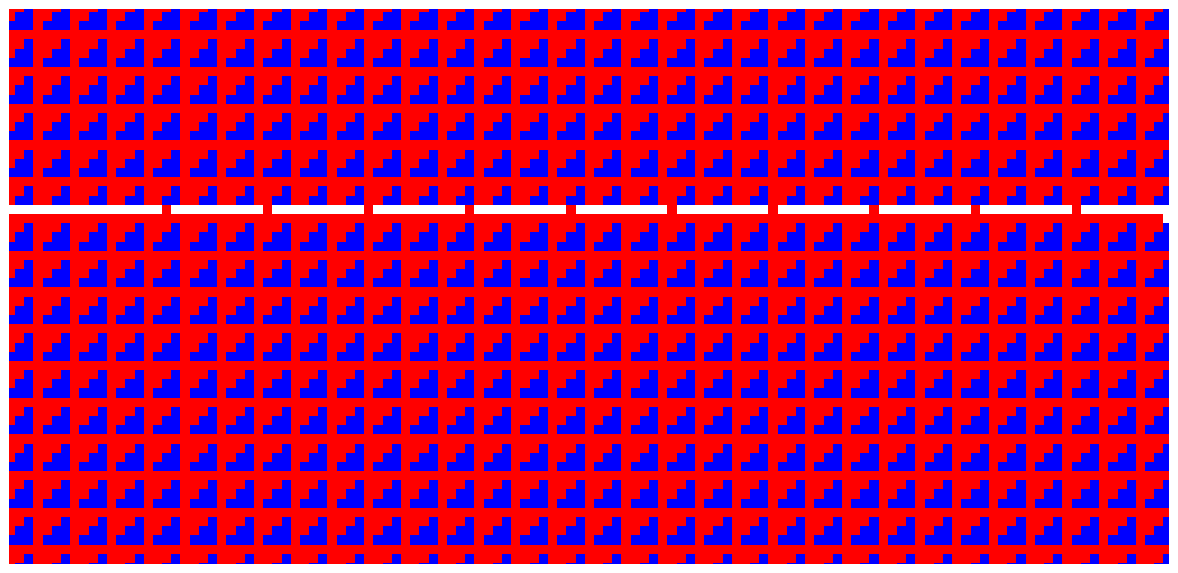
\includegraphics[width=\linewidth,height=.78\textheight,keepaspectratio]{figures/figure09.pdf}
\caption{Highway detail in the evolution of tile \eqref{eq:faultlines} at $n=1000$, $t=5000$.}
\label{fig:highway}
\end{figure}
The highways appear to increase the clearing time since regions near the right (and top) edge of the configuration which might ordinarily clear quickly are blocked by cars being moved by the highways. Moreover, as seen in Figure \ref{fig:fault_lines}, the highways tend to lead into fault-lines and vice-versa. Similar to the fault lines, as $n$ increases the number of highways increase. The proliferation of these fault-lines as $n$ increases provides a plausible mechanism for the observed superlinear clearing times.

\subsection{Reorganisation}
Reorganisation is the phenomena in which the blocked region containing the initial periodic configuration reorganises itself into a different periodic configuration with only a small proportion of the cars in this initial configuration moving. This reorganisation occurs quicker than cars clearing from the grid and so we reach a remarkably different configuration in the blocked region faster. An example which demonstrates reorganisation is the periodic configuration with tiling
\begin{equation}\label{eq:reorganisation}
\begin{split}
     \begin{tikzpicture}[scale=1.1]
        \rc{0}{0} \uc{0.6}{0} \uc{1.2}{0}
        \rc{0}{-0.6} \uc{0.6}{-0.6} \rc{1.2}{-0.6}
        \uc{0}{-1.2} \rc{0.6}{-1.2} \uc{1.2}{-1.2}
    \end{tikzpicture}
    \end{split}
\end{equation}
as shown in Figure \ref{fig:reorganisation}. A zoomed in image of the boundary between the $2$ regions can be seen in Figure \ref{fig:reorganisation_zoomed}.
\begin{figure}
\centering
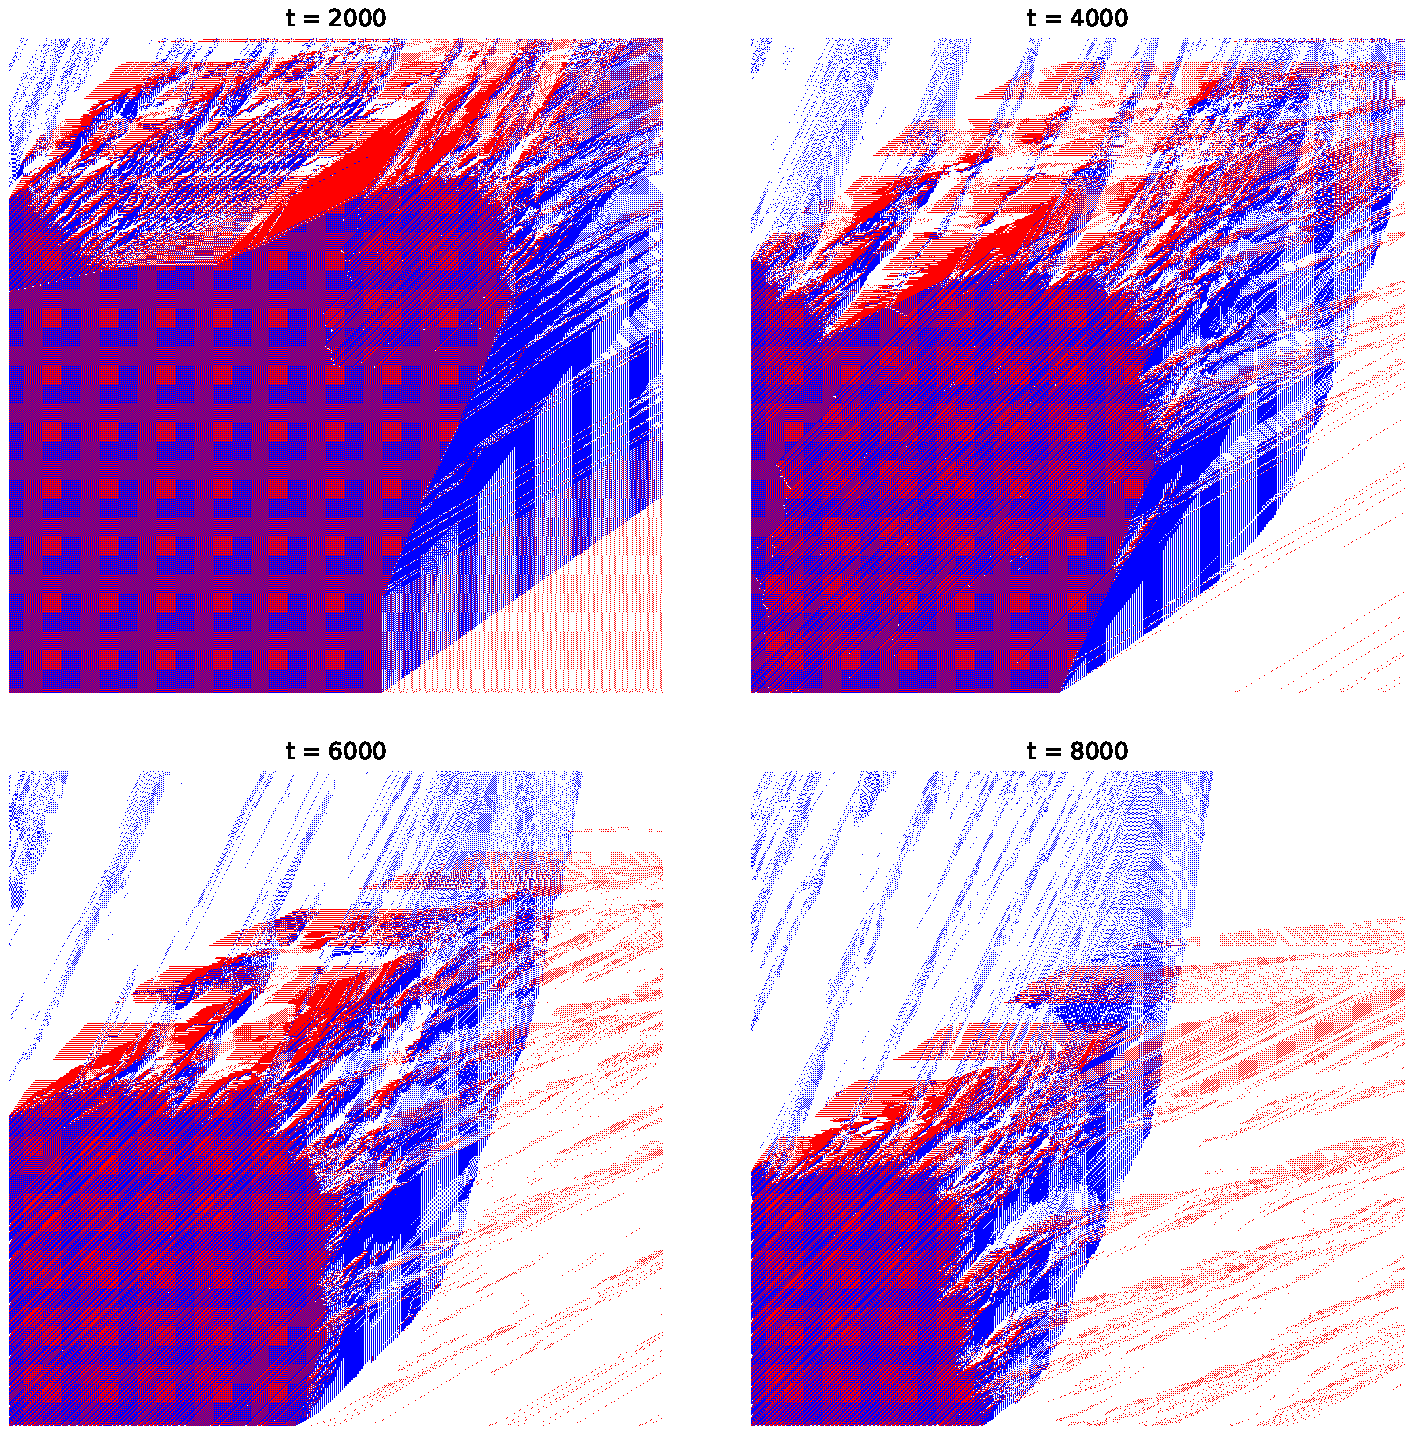
\includegraphics[width=\linewidth,height=.78\textheight,keepaspectratio]{figures/figure10.pdf}
\caption{Reorganisation of tile \eqref{eq:reorganisation} for $n=999$ at $t=2000,4000,6000,8000$.}
\label{fig:reorganisation}
\end{figure}
\begin{figure}
\centering
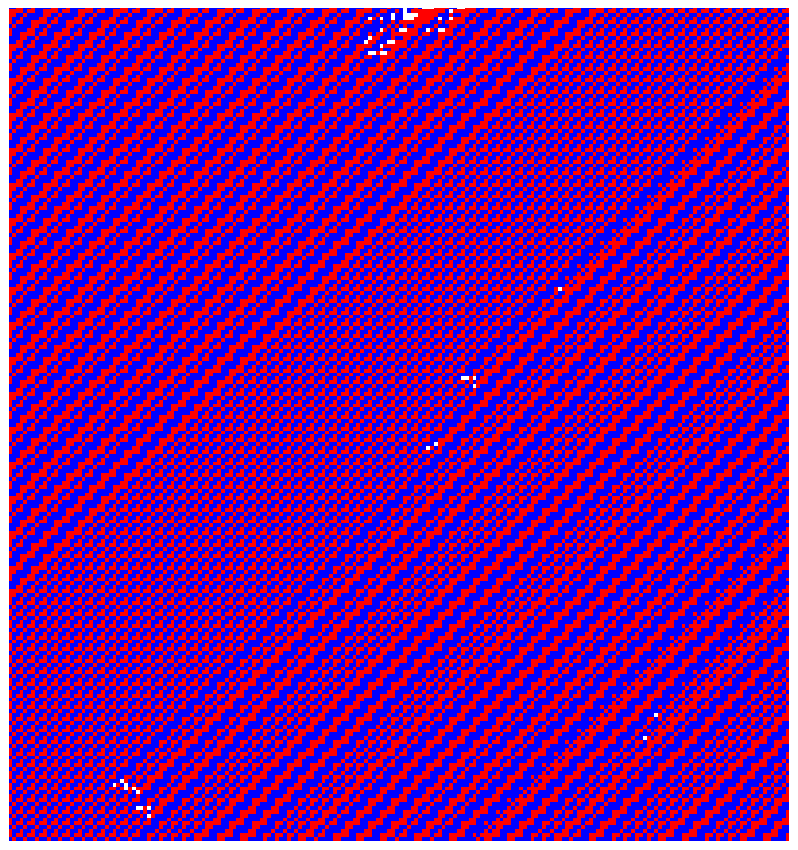
\includegraphics[width=\linewidth,height=.78\textheight,keepaspectratio]{figures/figure11.pdf}
\caption{Boundary detail in the evolution of tile \eqref{eq:reorganisation} at $n=999$, $t=4000$.}
\label{fig:reorganisation_zoomed}
\end{figure}
\section{Random Configurations}
We conclude with a discussion of configurations in the $n $-by-$ n$ grid initialised at random. In a sense these configurations characterise the typical clearing time of the BML model. In the simulations we consider configurations in which each site contains an $\ra$ with probability $\frac{1}{2}$ and a $\ua$ with probability $\frac{1}{2}$. We observe a clearing time with a power law as in the periodic configurations, albeit the evidence is less convincing and the conjectured power is smaller in the random configurations than in the periodic configurations. The data from simulations for random configurations is plotted in Figure \ref{fig:random_graphs}.
\begin{figure}
\centering
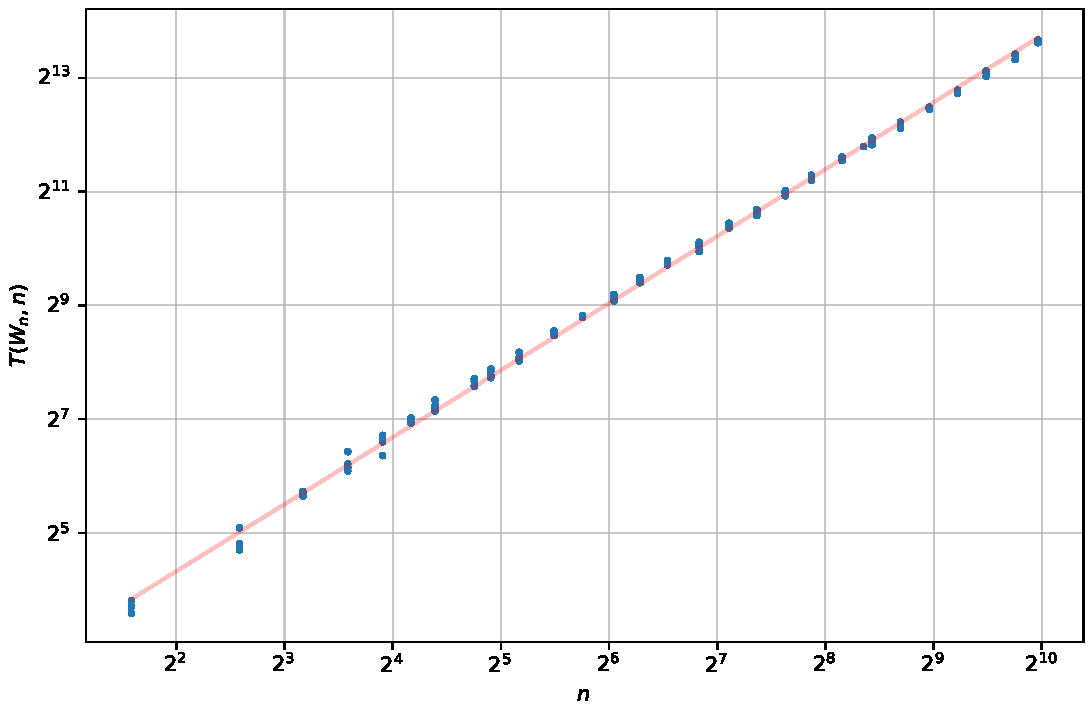
\includegraphics[width=\linewidth,height=.78\textheight,keepaspectratio]{figures/figure12.pdf}
\caption{Clearing times for seeded random configurations, using \FigureTwelveCount{} observations up to $n=\FigureTwelveMaxN$. Least-squares fit: $\log_2 T(W_n,n)=\FigureTwelvePower\log_2 n+\FigureTwelveIntercept$.}
\label{fig:random_graphs}
\end{figure}
Further, by inspecting the model midway through its clearing we notice the same chaotic clearing happening as seen in the periodic configurations, see Figure \ref{fig:random_1100}.
As a result it is natural to conclude that random configurations with high probability have asymptotically non-linear clearing times. However, the simulation evidence for random configurations is less convincing than in the periodic setting.
\begin{figure}
\centering
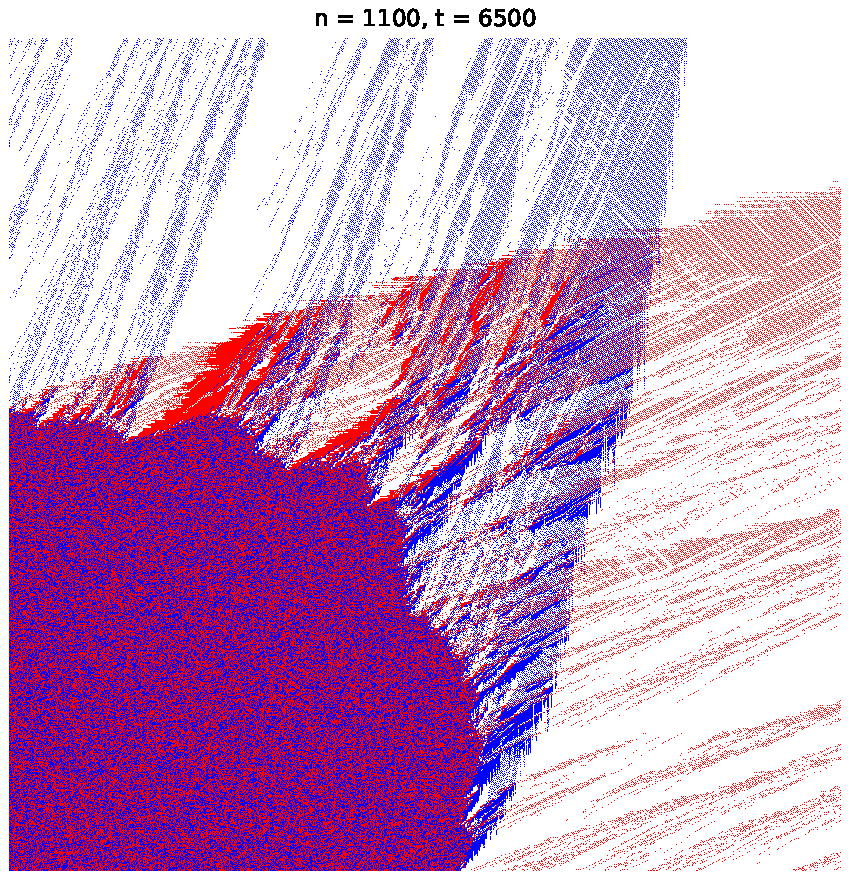
\includegraphics[width=\linewidth,height=.78\textheight,keepaspectratio]{figures/figure13.pdf}
\caption{A random configuration at $n=1100$, $t=6500$, evolved from the supplied initial matrix.}
\label{fig:random_1100}
\end{figure}

\clearpage
\appendix
\section{Vectorised Algorithm of the BML Model} \label{app:A}
Rows are indexed from top to bottom and columns from left to right;
$0$, $1$ and $3$ represent a vacant site, an East car and a North car,
respectively. The operators $\operatorname{shiftUp}$,
$\operatorname{shiftDown}$, $\operatorname{shiftLeft}$ and
$\operatorname{shiftRight}$ translate an array by one site, discard the
row or column that leaves the array, and fill the newly exposed row or
column with zeros.

\begingroup
\algrenewcommand{\algorithmicrequire}{\textbf{Input:}}
\algrenewcommand{\algorithmicensure}{\textbf{Output:}}
\begin{algorithm}[H]
\caption{One vectorised update of the BML model}
\label{alg:vectorised-bml}
\begin{algorithmic}[1]
\Require Configuration $G_{t-1}\in\{0,1,3\}^{n\times n}$ and integer $t\geq1$
\Ensure Configuration $G_t$ after the update at time $t$
\State $G\gets G_{t-1}$
\If{$t$ is odd}
    \State $S\gets\operatorname{shiftDown}(G)$
    \State $c\gets3$
\Else
    \State $S\gets\operatorname{shiftLeft}(G)$
    \State $c\gets1$
\EndIf
\State $I\gets G-S$
\State $B\gets0_{n\times n}$
\ForAll{$(i,j)\in[n]^2$}
    \If{$I(i,j)=c$}
        \State $B(i,j)\gets c$
    \EndIf
\EndFor
\If{$t$ is odd}
    \State $A\gets\operatorname{shiftUp}(B)$
\Else
    \State $A\gets\operatorname{shiftRight}(B)$
\EndIf
\State $N\gets G+A+B$
\ForAll{$(i,j)\in[n]^2$}
    \If{$N(i,j)=2c$}
        \State $N(i,j)\gets0$
    \EndIf
\EndFor
\State $G_t\gets N$
\State \Return $G_t$
\end{algorithmic}
\end{algorithm}
\endgroup

All shifts and masks are formed from the previous configuration before
any car positions are changed.

\section{Clearing formulas for periodic tilings}\label{app:survey}
The catalogue gives observed clearing formulas and conjectured power laws
for all $512$ $3$-periodic tilings, where $T=T(W_n,n)$ and $n$ is a multiple of $3$.
Red cells contain East cars and blue cells North cars.

\subsection{Affine and periodic formulas}
The following $235$ $3$-periodic tilings have affine or linear-plus-periodic
clearing formulas in the recorded data, where $P$ denotes
a periodic function that may depend on the tiling.
The formulas were determined using
$102\leq n\leq330$ and checked at every
$333\leq n\leq498$, with $n$ a multiple of $3$.

The linear coefficient $a$ is obtained from constant increments over repeated cycles,
giving the observed bound $T\leq an+\max P$.
A periodic correction is accepted when $T-an$ repeats on the fitting sizes
and agrees exactly with the validation data.
The formulas describe the tested sizes.

\noindent
% Tiling 111111111
\begin{minipage}[t]{.19\linewidth}\centering\vspace{0pt}
\resizebox{.96\linewidth}{!}{%
\begin{tikzpicture}
\rc{0}{0}
\rc{0.6}{0}
\rc{1.2}{0}
\rc{0}{-0.6}
\rc{0.6}{-0.6}
\rc{1.2}{-0.6}
\rc{0}{-1.2}
\rc{0.6}{-1.2}
\rc{1.2}{-1.2}
\end{tikzpicture}%
}
\par\smallskip
{\small\(T=4n-2\)\par}
\end{minipage}
\hfill
% Tiling 111111133
\begin{minipage}[t]{.19\linewidth}\centering\vspace{0pt}
\resizebox{.96\linewidth}{!}{%
\begin{tikzpicture}
\rc{0}{0}
\rc{0.6}{0}
\rc{1.2}{0}
\rc{0}{-0.6}
\rc{0.6}{-0.6}
\rc{1.2}{-0.6}
\rc{0}{-1.2}
\uc{0.6}{-1.2}
\uc{1.2}{-1.2}
\end{tikzpicture}%
}
\par\smallskip
{\small\(T=\frac{50}{9}n+P(n)\)\par}
\end{minipage}
\hfill
% Tiling 111111313
\begin{minipage}[t]{.19\linewidth}\centering\vspace{0pt}
\resizebox{.96\linewidth}{!}{%
\begin{tikzpicture}
\rc{0}{0}
\rc{0.6}{0}
\rc{1.2}{0}
\rc{0}{-0.6}
\rc{0.6}{-0.6}
\rc{1.2}{-0.6}
\uc{0}{-1.2}
\rc{0.6}{-1.2}
\uc{1.2}{-1.2}
\end{tikzpicture}%
}
\par\smallskip
{\small\(T=\frac{50}{9}n+P(n)\)\par}
\end{minipage}
\hfill
% Tiling 111111331
\begin{minipage}[t]{.19\linewidth}\centering\vspace{0pt}
\resizebox{.96\linewidth}{!}{%
\begin{tikzpicture}
\rc{0}{0}
\rc{0.6}{0}
\rc{1.2}{0}
\rc{0}{-0.6}
\rc{0.6}{-0.6}
\rc{1.2}{-0.6}
\uc{0}{-1.2}
\uc{0.6}{-1.2}
\rc{1.2}{-1.2}
\end{tikzpicture}%
}
\par\smallskip
{\small\(T=\frac{50}{9}n+P(n)\)\par}
\end{minipage}
\hfill
% Tiling 111111333
\begin{minipage}[t]{.19\linewidth}\centering\vspace{0pt}
\resizebox{.96\linewidth}{!}{%
\begin{tikzpicture}
\rc{0}{0}
\rc{0.6}{0}
\rc{1.2}{0}
\rc{0}{-0.6}
\rc{0.6}{-0.6}
\rc{1.2}{-0.6}
\uc{0}{-1.2}
\uc{0.6}{-1.2}
\uc{1.2}{-1.2}
\end{tikzpicture}%
}
\par\smallskip
{\small\(T=6n-1\)\par}
\end{minipage}
\par\vspace{.6em}
\noindent
% Tiling 111113113
\begin{minipage}[t]{.19\linewidth}\centering\vspace{0pt}
\resizebox{.96\linewidth}{!}{%
\begin{tikzpicture}
\rc{0}{0}
\rc{0.6}{0}
\rc{1.2}{0}
\rc{0}{-0.6}
\rc{0.6}{-0.6}
\uc{1.2}{-0.6}
\rc{0}{-1.2}
\rc{0.6}{-1.2}
\uc{1.2}{-1.2}
\end{tikzpicture}%
}
\par\smallskip
{\small\(T=\frac{20}{3}n-6\)\par}
\end{minipage}
\hfill
% Tiling 111113131
\begin{minipage}[t]{.19\linewidth}\centering\vspace{0pt}
\resizebox{.96\linewidth}{!}{%
\begin{tikzpicture}
\rc{0}{0}
\rc{0.6}{0}
\rc{1.2}{0}
\rc{0}{-0.6}
\rc{0.6}{-0.6}
\uc{1.2}{-0.6}
\rc{0}{-1.2}
\uc{0.6}{-1.2}
\rc{1.2}{-1.2}
\end{tikzpicture}%
}
\par\smallskip
{\small\(T=\frac{50}{9}n+P(n)\)\par}
\end{minipage}
\hfill
% Tiling 111113133
\begin{minipage}[t]{.19\linewidth}\centering\vspace{0pt}
\resizebox{.96\linewidth}{!}{%
\begin{tikzpicture}
\rc{0}{0}
\rc{0.6}{0}
\rc{1.2}{0}
\rc{0}{-0.6}
\rc{0.6}{-0.6}
\uc{1.2}{-0.6}
\rc{0}{-1.2}
\uc{0.6}{-1.2}
\uc{1.2}{-1.2}
\end{tikzpicture}%
}
\par\smallskip
{\small\(T=\frac{22}{3}n-8\)\par}
\end{minipage}
\hfill
% Tiling 111113311
\begin{minipage}[t]{.19\linewidth}\centering\vspace{0pt}
\resizebox{.96\linewidth}{!}{%
\begin{tikzpicture}
\rc{0}{0}
\rc{0.6}{0}
\rc{1.2}{0}
\rc{0}{-0.6}
\rc{0.6}{-0.6}
\uc{1.2}{-0.6}
\uc{0}{-1.2}
\rc{0.6}{-1.2}
\rc{1.2}{-1.2}
\end{tikzpicture}%
}
\par\smallskip
{\small\(T=\frac{50}{9}n+P(n)\)\par}
\end{minipage}
\hfill
% Tiling 111113331
\begin{minipage}[t]{.19\linewidth}\centering\vspace{0pt}
\resizebox{.96\linewidth}{!}{%
\begin{tikzpicture}
\rc{0}{0}
\rc{0.6}{0}
\rc{1.2}{0}
\rc{0}{-0.6}
\rc{0.6}{-0.6}
\uc{1.2}{-0.6}
\uc{0}{-1.2}
\uc{0.6}{-1.2}
\rc{1.2}{-1.2}
\end{tikzpicture}%
}
\par\smallskip
{\small\(T=6n-4\)\par}
\end{minipage}
\par\vspace{.6em}
\noindent
% Tiling 111131113
\begin{minipage}[t]{.19\linewidth}\centering\vspace{0pt}
\resizebox{.96\linewidth}{!}{%
\begin{tikzpicture}
\rc{0}{0}
\rc{0.6}{0}
\rc{1.2}{0}
\rc{0}{-0.6}
\uc{0.6}{-0.6}
\rc{1.2}{-0.6}
\rc{0}{-1.2}
\rc{0.6}{-1.2}
\uc{1.2}{-1.2}
\end{tikzpicture}%
}
\par\smallskip
{\small\(T=\frac{50}{9}n+P(n)\)\par}
\end{minipage}
\hfill
% Tiling 111131131
\begin{minipage}[t]{.19\linewidth}\centering\vspace{0pt}
\resizebox{.96\linewidth}{!}{%
\begin{tikzpicture}
\rc{0}{0}
\rc{0.6}{0}
\rc{1.2}{0}
\rc{0}{-0.6}
\uc{0.6}{-0.6}
\rc{1.2}{-0.6}
\rc{0}{-1.2}
\uc{0.6}{-1.2}
\rc{1.2}{-1.2}
\end{tikzpicture}%
}
\par\smallskip
{\small\(T=\frac{20}{3}n-6\)\par}
\end{minipage}
\hfill
% Tiling 111131311
\begin{minipage}[t]{.19\linewidth}\centering\vspace{0pt}
\resizebox{.96\linewidth}{!}{%
\begin{tikzpicture}
\rc{0}{0}
\rc{0.6}{0}
\rc{1.2}{0}
\rc{0}{-0.6}
\uc{0.6}{-0.6}
\rc{1.2}{-0.6}
\uc{0}{-1.2}
\rc{0.6}{-1.2}
\rc{1.2}{-1.2}
\end{tikzpicture}%
}
\par\smallskip
{\small\(T=\frac{50}{9}n+P(n)\)\par}
\end{minipage}
\hfill
% Tiling 111131313
\begin{minipage}[t]{.19\linewidth}\centering\vspace{0pt}
\resizebox{.96\linewidth}{!}{%
\begin{tikzpicture}
\rc{0}{0}
\rc{0.6}{0}
\rc{1.2}{0}
\rc{0}{-0.6}
\uc{0.6}{-0.6}
\rc{1.2}{-0.6}
\uc{0}{-1.2}
\rc{0.6}{-1.2}
\uc{1.2}{-1.2}
\end{tikzpicture}%
}
\par\smallskip
{\small\(T=6n-6\)\par}
\end{minipage}
\hfill
% Tiling 111131331
\begin{minipage}[t]{.19\linewidth}\centering\vspace{0pt}
\resizebox{.96\linewidth}{!}{%
\begin{tikzpicture}
\rc{0}{0}
\rc{0.6}{0}
\rc{1.2}{0}
\rc{0}{-0.6}
\uc{0.6}{-0.6}
\rc{1.2}{-0.6}
\uc{0}{-1.2}
\uc{0.6}{-1.2}
\rc{1.2}{-1.2}
\end{tikzpicture}%
}
\par\smallskip
{\small\(T=\frac{22}{3}n-9\)\par}
\end{minipage}
\par\vspace{.6em}
\noindent
% Tiling 111133111
\begin{minipage}[t]{.19\linewidth}\centering\vspace{0pt}
\resizebox{.96\linewidth}{!}{%
\begin{tikzpicture}
\rc{0}{0}
\rc{0.6}{0}
\rc{1.2}{0}
\rc{0}{-0.6}
\uc{0.6}{-0.6}
\uc{1.2}{-0.6}
\rc{0}{-1.2}
\rc{0.6}{-1.2}
\rc{1.2}{-1.2}
\end{tikzpicture}%
}
\par\smallskip
{\small\(T=\frac{50}{9}n+P(n)\)\par}
\end{minipage}
\hfill
% Tiling 111133133
\begin{minipage}[t]{.19\linewidth}\centering\vspace{0pt}
\resizebox{.96\linewidth}{!}{%
\begin{tikzpicture}
\rc{0}{0}
\rc{0.6}{0}
\rc{1.2}{0}
\rc{0}{-0.6}
\uc{0.6}{-0.6}
\uc{1.2}{-0.6}
\rc{0}{-1.2}
\uc{0.6}{-1.2}
\uc{1.2}{-1.2}
\end{tikzpicture}%
}
\par\smallskip
{\small\(T=\frac{22}{3}n-6\)\par}
\end{minipage}
\hfill
% Tiling 111133311
\begin{minipage}[t]{.19\linewidth}\centering\vspace{0pt}
\resizebox{.96\linewidth}{!}{%
\begin{tikzpicture}
\rc{0}{0}
\rc{0.6}{0}
\rc{1.2}{0}
\rc{0}{-0.6}
\uc{0.6}{-0.6}
\uc{1.2}{-0.6}
\uc{0}{-1.2}
\rc{0.6}{-1.2}
\rc{1.2}{-1.2}
\end{tikzpicture}%
}
\par\smallskip
{\small\(T=6n-2\)\par}
\end{minipage}
\hfill
% Tiling 111311113
\begin{minipage}[t]{.19\linewidth}\centering\vspace{0pt}
\resizebox{.96\linewidth}{!}{%
\begin{tikzpicture}
\rc{0}{0}
\rc{0.6}{0}
\rc{1.2}{0}
\uc{0}{-0.6}
\rc{0.6}{-0.6}
\rc{1.2}{-0.6}
\rc{0}{-1.2}
\rc{0.6}{-1.2}
\uc{1.2}{-1.2}
\end{tikzpicture}%
}
\par\smallskip
{\small\(T=\frac{16}{3}n-2\)\par}
\end{minipage}
\hfill
% Tiling 111311131
\begin{minipage}[t]{.19\linewidth}\centering\vspace{0pt}
\resizebox{.96\linewidth}{!}{%
\begin{tikzpicture}
\rc{0}{0}
\rc{0.6}{0}
\rc{1.2}{0}
\uc{0}{-0.6}
\rc{0.6}{-0.6}
\rc{1.2}{-0.6}
\rc{0}{-1.2}
\uc{0.6}{-1.2}
\rc{1.2}{-1.2}
\end{tikzpicture}%
}
\par\smallskip
{\small\(T=\frac{50}{9}n+P(n)\)\par}
\end{minipage}
\par\vspace{.6em}
\noindent
% Tiling 111311133
\begin{minipage}[t]{.19\linewidth}\centering\vspace{0pt}
\resizebox{.96\linewidth}{!}{%
\begin{tikzpicture}
\rc{0}{0}
\rc{0.6}{0}
\rc{1.2}{0}
\uc{0}{-0.6}
\rc{0.6}{-0.6}
\rc{1.2}{-0.6}
\rc{0}{-1.2}
\uc{0.6}{-1.2}
\uc{1.2}{-1.2}
\end{tikzpicture}%
}
\par\smallskip
{\small\(T=6n-6\)\par}
\end{minipage}
\hfill
% Tiling 111311311
\begin{minipage}[t]{.19\linewidth}\centering\vspace{0pt}
\resizebox{.96\linewidth}{!}{%
\begin{tikzpicture}
\rc{0}{0}
\rc{0.6}{0}
\rc{1.2}{0}
\uc{0}{-0.6}
\rc{0.6}{-0.6}
\rc{1.2}{-0.6}
\uc{0}{-1.2}
\rc{0.6}{-1.2}
\rc{1.2}{-1.2}
\end{tikzpicture}%
}
\par\smallskip
{\small\(T=\frac{20}{3}n-7\)\par}
\end{minipage}
\hfill
% Tiling 111311313
\begin{minipage}[t]{.19\linewidth}\centering\vspace{0pt}
\resizebox{.96\linewidth}{!}{%
\begin{tikzpicture}
\rc{0}{0}
\rc{0.6}{0}
\rc{1.2}{0}
\uc{0}{-0.6}
\rc{0.6}{-0.6}
\rc{1.2}{-0.6}
\uc{0}{-1.2}
\rc{0.6}{-1.2}
\uc{1.2}{-1.2}
\end{tikzpicture}%
}
\par\smallskip
{\small\(T=\frac{22}{3}n-9\)\par}
\end{minipage}
\hfill
% Tiling 111313111
\begin{minipage}[t]{.19\linewidth}\centering\vspace{0pt}
\resizebox{.96\linewidth}{!}{%
\begin{tikzpicture}
\rc{0}{0}
\rc{0.6}{0}
\rc{1.2}{0}
\uc{0}{-0.6}
\rc{0.6}{-0.6}
\uc{1.2}{-0.6}
\rc{0}{-1.2}
\rc{0.6}{-1.2}
\rc{1.2}{-1.2}
\end{tikzpicture}%
}
\par\smallskip
{\small\(T=\frac{50}{9}n+P(n)\)\par}
\end{minipage}
\hfill
% Tiling 111313131
\begin{minipage}[t]{.19\linewidth}\centering\vspace{0pt}
\resizebox{.96\linewidth}{!}{%
\begin{tikzpicture}
\rc{0}{0}
\rc{0.6}{0}
\rc{1.2}{0}
\uc{0}{-0.6}
\rc{0.6}{-0.6}
\uc{1.2}{-0.6}
\rc{0}{-1.2}
\uc{0.6}{-1.2}
\rc{1.2}{-1.2}
\end{tikzpicture}%
}
\par\smallskip
{\small\(T=6n-4\)\par}
\end{minipage}
\par\vspace{.6em}
\noindent
% Tiling 111313313
\begin{minipage}[t]{.19\linewidth}\centering\vspace{0pt}
\resizebox{.96\linewidth}{!}{%
\begin{tikzpicture}
\rc{0}{0}
\rc{0.6}{0}
\rc{1.2}{0}
\uc{0}{-0.6}
\rc{0.6}{-0.6}
\uc{1.2}{-0.6}
\uc{0}{-1.2}
\rc{0.6}{-1.2}
\uc{1.2}{-1.2}
\end{tikzpicture}%
}
\par\smallskip
{\small\(T=\frac{22}{3}n-7\)\par}
\end{minipage}
\hfill
% Tiling 111331111
\begin{minipage}[t]{.19\linewidth}\centering\vspace{0pt}
\resizebox{.96\linewidth}{!}{%
\begin{tikzpicture}
\rc{0}{0}
\rc{0.6}{0}
\rc{1.2}{0}
\uc{0}{-0.6}
\uc{0.6}{-0.6}
\rc{1.2}{-0.6}
\rc{0}{-1.2}
\rc{0.6}{-1.2}
\rc{1.2}{-1.2}
\end{tikzpicture}%
}
\par\smallskip
{\small\(T=\frac{50}{9}n+P(n)\)\par}
\end{minipage}
\hfill
% Tiling 111331113
\begin{minipage}[t]{.19\linewidth}\centering\vspace{0pt}
\resizebox{.96\linewidth}{!}{%
\begin{tikzpicture}
\rc{0}{0}
\rc{0.6}{0}
\rc{1.2}{0}
\uc{0}{-0.6}
\uc{0.6}{-0.6}
\rc{1.2}{-0.6}
\rc{0}{-1.2}
\rc{0.6}{-1.2}
\uc{1.2}{-1.2}
\end{tikzpicture}%
}
\par\smallskip
{\small\(T=6n-4\)\par}
\end{minipage}
\hfill
% Tiling 111331331
\begin{minipage}[t]{.19\linewidth}\centering\vspace{0pt}
\resizebox{.96\linewidth}{!}{%
\begin{tikzpicture}
\rc{0}{0}
\rc{0.6}{0}
\rc{1.2}{0}
\uc{0}{-0.6}
\uc{0.6}{-0.6}
\rc{1.2}{-0.6}
\uc{0}{-1.2}
\uc{0.6}{-1.2}
\rc{1.2}{-1.2}
\end{tikzpicture}%
}
\par\smallskip
{\small\(T=\frac{22}{3}n-7\)\par}
\end{minipage}
\hfill
% Tiling 111333111
\begin{minipage}[t]{.19\linewidth}\centering\vspace{0pt}
\resizebox{.96\linewidth}{!}{%
\begin{tikzpicture}
\rc{0}{0}
\rc{0.6}{0}
\rc{1.2}{0}
\uc{0}{-0.6}
\uc{0.6}{-0.6}
\uc{1.2}{-0.6}
\rc{0}{-1.2}
\rc{0.6}{-1.2}
\rc{1.2}{-1.2}
\end{tikzpicture}%
}
\par\smallskip
{\small\(T=6n-2\)\par}
\end{minipage}
\par\vspace{.6em}
\noindent
% Tiling 111333333
\begin{minipage}[t]{.19\linewidth}\centering\vspace{0pt}
\resizebox{.96\linewidth}{!}{%
\begin{tikzpicture}
\rc{0}{0}
\rc{0.6}{0}
\rc{1.2}{0}
\uc{0}{-0.6}
\uc{0.6}{-0.6}
\uc{1.2}{-0.6}
\uc{0}{-1.2}
\uc{0.6}{-1.2}
\uc{1.2}{-1.2}
\end{tikzpicture}%
}
\par\smallskip
{\small\(T=\frac{20}{3}n-3\)\par}
\end{minipage}
\hfill
% Tiling 113111113
\begin{minipage}[t]{.19\linewidth}\centering\vspace{0pt}
\resizebox{.96\linewidth}{!}{%
\begin{tikzpicture}
\rc{0}{0}
\rc{0.6}{0}
\uc{1.2}{0}
\rc{0}{-0.6}
\rc{0.6}{-0.6}
\rc{1.2}{-0.6}
\rc{0}{-1.2}
\rc{0.6}{-1.2}
\uc{1.2}{-1.2}
\end{tikzpicture}%
}
\par\smallskip
{\small\(T=\frac{20}{3}n-8\)\par}
\end{minipage}
\hfill
% Tiling 113111131
\begin{minipage}[t]{.19\linewidth}\centering\vspace{0pt}
\resizebox{.96\linewidth}{!}{%
\begin{tikzpicture}
\rc{0}{0}
\rc{0.6}{0}
\uc{1.2}{0}
\rc{0}{-0.6}
\rc{0.6}{-0.6}
\rc{1.2}{-0.6}
\rc{0}{-1.2}
\uc{0.6}{-1.2}
\rc{1.2}{-1.2}
\end{tikzpicture}%
}
\par\smallskip
{\small\(T=\frac{50}{9}n+P(n)\)\par}
\end{minipage}
\hfill
% Tiling 113111311
\begin{minipage}[t]{.19\linewidth}\centering\vspace{0pt}
\resizebox{.96\linewidth}{!}{%
\begin{tikzpicture}
\rc{0}{0}
\rc{0.6}{0}
\uc{1.2}{0}
\rc{0}{-0.6}
\rc{0.6}{-0.6}
\rc{1.2}{-0.6}
\uc{0}{-1.2}
\rc{0.6}{-1.2}
\rc{1.2}{-1.2}
\end{tikzpicture}%
}
\par\smallskip
{\small\(T=\frac{16}{3}n-2\)\par}
\end{minipage}
\hfill
% Tiling 113111331
\begin{minipage}[t]{.19\linewidth}\centering\vspace{0pt}
\resizebox{.96\linewidth}{!}{%
\begin{tikzpicture}
\rc{0}{0}
\rc{0.6}{0}
\uc{1.2}{0}
\rc{0}{-0.6}
\rc{0.6}{-0.6}
\rc{1.2}{-0.6}
\uc{0}{-1.2}
\uc{0.6}{-1.2}
\rc{1.2}{-1.2}
\end{tikzpicture}%
}
\par\smallskip
{\small\(T=6n-4\)\par}
\end{minipage}
\par\vspace{.6em}
\noindent
% Tiling 113113111
\begin{minipage}[t]{.19\linewidth}\centering\vspace{0pt}
\resizebox{.96\linewidth}{!}{%
\begin{tikzpicture}
\rc{0}{0}
\rc{0.6}{0}
\uc{1.2}{0}
\rc{0}{-0.6}
\rc{0.6}{-0.6}
\uc{1.2}{-0.6}
\rc{0}{-1.2}
\rc{0.6}{-1.2}
\rc{1.2}{-1.2}
\end{tikzpicture}%
}
\par\smallskip
{\small\(T=\frac{20}{3}n-8\)\par}
\end{minipage}
\hfill
% Tiling 113113113
\begin{minipage}[t]{.19\linewidth}\centering\vspace{0pt}
\resizebox{.96\linewidth}{!}{%
\begin{tikzpicture}
\rc{0}{0}
\rc{0.6}{0}
\uc{1.2}{0}
\rc{0}{-0.6}
\rc{0.6}{-0.6}
\uc{1.2}{-0.6}
\rc{0}{-1.2}
\rc{0.6}{-1.2}
\uc{1.2}{-1.2}
\end{tikzpicture}%
}
\par\smallskip
{\small\(T=\frac{20}{3}n-4\)\par}
\end{minipage}
\hfill
% Tiling 113113131
\begin{minipage}[t]{.19\linewidth}\centering\vspace{0pt}
\resizebox{.96\linewidth}{!}{%
\begin{tikzpicture}
\rc{0}{0}
\rc{0.6}{0}
\uc{1.2}{0}
\rc{0}{-0.6}
\rc{0.6}{-0.6}
\uc{1.2}{-0.6}
\rc{0}{-1.2}
\uc{0.6}{-1.2}
\rc{1.2}{-1.2}
\end{tikzpicture}%
}
\par\smallskip
{\small\(T=\frac{16}{3}n-2\)\par}
\end{minipage}
\hfill
% Tiling 113113311
\begin{minipage}[t]{.19\linewidth}\centering\vspace{0pt}
\resizebox{.96\linewidth}{!}{%
\begin{tikzpicture}
\rc{0}{0}
\rc{0.6}{0}
\uc{1.2}{0}
\rc{0}{-0.6}
\rc{0.6}{-0.6}
\uc{1.2}{-0.6}
\uc{0}{-1.2}
\rc{0.6}{-1.2}
\rc{1.2}{-1.2}
\end{tikzpicture}%
}
\par\smallskip
{\small\(T=\frac{16}{3}n-1\)\par}
\end{minipage}
\hfill
% Tiling 113113333
\begin{minipage}[t]{.19\linewidth}\centering\vspace{0pt}
\resizebox{.96\linewidth}{!}{%
\begin{tikzpicture}
\rc{0}{0}
\rc{0.6}{0}
\uc{1.2}{0}
\rc{0}{-0.6}
\rc{0.6}{-0.6}
\uc{1.2}{-0.6}
\uc{0}{-1.2}
\uc{0.6}{-1.2}
\uc{1.2}{-1.2}
\end{tikzpicture}%
}
\par\smallskip
{\small\(T=\frac{22}{3}n-7\)\par}
\end{minipage}
\par\vspace{.6em}
\noindent
% Tiling 113131111
\begin{minipage}[t]{.19\linewidth}\centering\vspace{0pt}
\resizebox{.96\linewidth}{!}{%
\begin{tikzpicture}
\rc{0}{0}
\rc{0.6}{0}
\uc{1.2}{0}
\rc{0}{-0.6}
\uc{0.6}{-0.6}
\rc{1.2}{-0.6}
\rc{0}{-1.2}
\rc{0.6}{-1.2}
\rc{1.2}{-1.2}
\end{tikzpicture}%
}
\par\smallskip
{\small\(T=\frac{50}{9}n+P(n)\)\par}
\end{minipage}
\hfill
% Tiling 113131113
\begin{minipage}[t]{.19\linewidth}\centering\vspace{0pt}
\resizebox{.96\linewidth}{!}{%
\begin{tikzpicture}
\rc{0}{0}
\rc{0.6}{0}
\uc{1.2}{0}
\rc{0}{-0.6}
\uc{0.6}{-0.6}
\rc{1.2}{-0.6}
\rc{0}{-1.2}
\rc{0.6}{-1.2}
\uc{1.2}{-1.2}
\end{tikzpicture}%
}
\par\smallskip
{\small\(T=\frac{16}{3}n-6\)\par}
\end{minipage}
\hfill
% Tiling 113131131
\begin{minipage}[t]{.19\linewidth}\centering\vspace{0pt}
\resizebox{.96\linewidth}{!}{%
\begin{tikzpicture}
\rc{0}{0}
\rc{0.6}{0}
\uc{1.2}{0}
\rc{0}{-0.6}
\uc{0.6}{-0.6}
\rc{1.2}{-0.6}
\rc{0}{-1.2}
\uc{0.6}{-1.2}
\rc{1.2}{-1.2}
\end{tikzpicture}%
}
\par\smallskip
{\small\(T=\frac{16}{3}n-2\)\par}
\end{minipage}
\hfill
% Tiling 113131133
\begin{minipage}[t]{.19\linewidth}\centering\vspace{0pt}
\resizebox{.96\linewidth}{!}{%
\begin{tikzpicture}
\rc{0}{0}
\rc{0.6}{0}
\uc{1.2}{0}
\rc{0}{-0.6}
\uc{0.6}{-0.6}
\rc{1.2}{-0.6}
\rc{0}{-1.2}
\uc{0.6}{-1.2}
\uc{1.2}{-1.2}
\end{tikzpicture}%
}
\par\smallskip
{\small\(T=\frac{146}{27}n+P(n)\)\par}
\end{minipage}
\hfill
% Tiling 113131311
\begin{minipage}[t]{.19\linewidth}\centering\vspace{0pt}
\resizebox{.96\linewidth}{!}{%
\begin{tikzpicture}
\rc{0}{0}
\rc{0.6}{0}
\uc{1.2}{0}
\rc{0}{-0.6}
\uc{0.6}{-0.6}
\rc{1.2}{-0.6}
\uc{0}{-1.2}
\rc{0.6}{-1.2}
\rc{1.2}{-1.2}
\end{tikzpicture}%
}
\par\smallskip
{\small\(T=4n\)\par}
\end{minipage}
\par\vspace{.6em}
\noindent
% Tiling 113131333
\begin{minipage}[t]{.19\linewidth}\centering\vspace{0pt}
\resizebox{.96\linewidth}{!}{%
\begin{tikzpicture}
\rc{0}{0}
\rc{0.6}{0}
\uc{1.2}{0}
\rc{0}{-0.6}
\uc{0.6}{-0.6}
\rc{1.2}{-0.6}
\uc{0}{-1.2}
\uc{0.6}{-1.2}
\uc{1.2}{-1.2}
\end{tikzpicture}%
}
\par\smallskip
{\small\(T=\frac{146}{27}n+P(n)\)\par}
\end{minipage}
\hfill
% Tiling 113133131
\begin{minipage}[t]{.19\linewidth}\centering\vspace{0pt}
\resizebox{.96\linewidth}{!}{%
\begin{tikzpicture}
\rc{0}{0}
\rc{0.6}{0}
\uc{1.2}{0}
\rc{0}{-0.6}
\uc{0.6}{-0.6}
\uc{1.2}{-0.6}
\rc{0}{-1.2}
\uc{0.6}{-1.2}
\rc{1.2}{-1.2}
\end{tikzpicture}%
}
\par\smallskip
{\small\(T=\frac{146}{27}n+P(n)\)\par}
\end{minipage}
\hfill
% Tiling 113133333
\begin{minipage}[t]{.19\linewidth}\centering\vspace{0pt}
\resizebox{.96\linewidth}{!}{%
\begin{tikzpicture}
\rc{0}{0}
\rc{0.6}{0}
\uc{1.2}{0}
\rc{0}{-0.6}
\uc{0.6}{-0.6}
\uc{1.2}{-0.6}
\uc{0}{-1.2}
\uc{0.6}{-1.2}
\uc{1.2}{-1.2}
\end{tikzpicture}%
}
\par\smallskip
{\small\(T=\frac{22}{3}n-9\)\par}
\end{minipage}
\hfill
% Tiling 113311111
\begin{minipage}[t]{.19\linewidth}\centering\vspace{0pt}
\resizebox{.96\linewidth}{!}{%
\begin{tikzpicture}
\rc{0}{0}
\rc{0.6}{0}
\uc{1.2}{0}
\uc{0}{-0.6}
\rc{0.6}{-0.6}
\rc{1.2}{-0.6}
\rc{0}{-1.2}
\rc{0.6}{-1.2}
\rc{1.2}{-1.2}
\end{tikzpicture}%
}
\par\smallskip
{\small\(T=\frac{50}{9}n+P(n)\)\par}
\end{minipage}
\hfill
% Tiling 113311113
\begin{minipage}[t]{.19\linewidth}\centering\vspace{0pt}
\resizebox{.96\linewidth}{!}{%
\begin{tikzpicture}
\rc{0}{0}
\rc{0.6}{0}
\uc{1.2}{0}
\uc{0}{-0.6}
\rc{0.6}{-0.6}
\rc{1.2}{-0.6}
\rc{0}{-1.2}
\rc{0.6}{-1.2}
\uc{1.2}{-1.2}
\end{tikzpicture}%
}
\par\smallskip
{\small\(T=\frac{16}{3}n-6\)\par}
\end{minipage}
\par\vspace{.6em}
\noindent
% Tiling 113311131
\begin{minipage}[t]{.19\linewidth}\centering\vspace{0pt}
\resizebox{.96\linewidth}{!}{%
\begin{tikzpicture}
\rc{0}{0}
\rc{0.6}{0}
\uc{1.2}{0}
\uc{0}{-0.6}
\rc{0.6}{-0.6}
\rc{1.2}{-0.6}
\rc{0}{-1.2}
\uc{0.6}{-1.2}
\rc{1.2}{-1.2}
\end{tikzpicture}%
}
\par\smallskip
{\small\(T=4n-1\)\par}
\end{minipage}
\hfill
% Tiling 113311311
\begin{minipage}[t]{.19\linewidth}\centering\vspace{0pt}
\resizebox{.96\linewidth}{!}{%
\begin{tikzpicture}
\rc{0}{0}
\rc{0.6}{0}
\uc{1.2}{0}
\uc{0}{-0.6}
\rc{0.6}{-0.6}
\rc{1.2}{-0.6}
\uc{0}{-1.2}
\rc{0.6}{-1.2}
\rc{1.2}{-1.2}
\end{tikzpicture}%
}
\par\smallskip
{\small\(T=\frac{16}{3}n-5\)\par}
\end{minipage}
\hfill
% Tiling 113311313
\begin{minipage}[t]{.19\linewidth}\centering\vspace{0pt}
\resizebox{.96\linewidth}{!}{%
\begin{tikzpicture}
\rc{0}{0}
\rc{0.6}{0}
\uc{1.2}{0}
\uc{0}{-0.6}
\rc{0.6}{-0.6}
\rc{1.2}{-0.6}
\uc{0}{-1.2}
\rc{0.6}{-1.2}
\uc{1.2}{-1.2}
\end{tikzpicture}%
}
\par\smallskip
{\small\(T=\frac{146}{27}n+P(n)\)\par}
\end{minipage}
\hfill
% Tiling 113311333
\begin{minipage}[t]{.19\linewidth}\centering\vspace{0pt}
\resizebox{.96\linewidth}{!}{%
\begin{tikzpicture}
\rc{0}{0}
\rc{0.6}{0}
\uc{1.2}{0}
\uc{0}{-0.6}
\rc{0.6}{-0.6}
\rc{1.2}{-0.6}
\uc{0}{-1.2}
\uc{0.6}{-1.2}
\uc{1.2}{-1.2}
\end{tikzpicture}%
}
\par\smallskip
{\small\(T=\frac{146}{27}n+P(n)\)\par}
\end{minipage}
\hfill
% Tiling 113313311
\begin{minipage}[t]{.19\linewidth}\centering\vspace{0pt}
\resizebox{.96\linewidth}{!}{%
\begin{tikzpicture}
\rc{0}{0}
\rc{0.6}{0}
\uc{1.2}{0}
\uc{0}{-0.6}
\rc{0.6}{-0.6}
\uc{1.2}{-0.6}
\uc{0}{-1.2}
\rc{0.6}{-1.2}
\rc{1.2}{-1.2}
\end{tikzpicture}%
}
\par\smallskip
{\small\(T=\frac{146}{27}n+P(n)\)\par}
\end{minipage}
\par\vspace{.6em}
\noindent
% Tiling 113331111
\begin{minipage}[t]{.19\linewidth}\centering\vspace{0pt}
\resizebox{.96\linewidth}{!}{%
\begin{tikzpicture}
\rc{0}{0}
\rc{0.6}{0}
\uc{1.2}{0}
\uc{0}{-0.6}
\uc{0.6}{-0.6}
\rc{1.2}{-0.6}
\rc{0}{-1.2}
\rc{0.6}{-1.2}
\rc{1.2}{-1.2}
\end{tikzpicture}%
}
\par\smallskip
{\small\(T=6n-4\)\par}
\end{minipage}
\hfill
% Tiling 113331333
\begin{minipage}[t]{.19\linewidth}\centering\vspace{0pt}
\resizebox{.96\linewidth}{!}{%
\begin{tikzpicture}
\rc{0}{0}
\rc{0.6}{0}
\uc{1.2}{0}
\uc{0}{-0.6}
\uc{0.6}{-0.6}
\rc{1.2}{-0.6}
\uc{0}{-1.2}
\uc{0.6}{-1.2}
\uc{1.2}{-1.2}
\end{tikzpicture}%
}
\par\smallskip
{\small\(T=\frac{16}{3}n-3\)\par}
\end{minipage}
\hfill
% Tiling 113333113
\begin{minipage}[t]{.19\linewidth}\centering\vspace{0pt}
\resizebox{.96\linewidth}{!}{%
\begin{tikzpicture}
\rc{0}{0}
\rc{0.6}{0}
\uc{1.2}{0}
\uc{0}{-0.6}
\uc{0.6}{-0.6}
\uc{1.2}{-0.6}
\rc{0}{-1.2}
\rc{0.6}{-1.2}
\uc{1.2}{-1.2}
\end{tikzpicture}%
}
\par\smallskip
{\small\(T=\frac{22}{3}n-8\)\par}
\end{minipage}
\hfill
% Tiling 113333131
\begin{minipage}[t]{.19\linewidth}\centering\vspace{0pt}
\resizebox{.96\linewidth}{!}{%
\begin{tikzpicture}
\rc{0}{0}
\rc{0.6}{0}
\uc{1.2}{0}
\uc{0}{-0.6}
\uc{0.6}{-0.6}
\uc{1.2}{-0.6}
\rc{0}{-1.2}
\uc{0.6}{-1.2}
\rc{1.2}{-1.2}
\end{tikzpicture}%
}
\par\smallskip
{\small\(T=\frac{16}{3}n-5\)\par}
\end{minipage}
\hfill
% Tiling 113333311
\begin{minipage}[t]{.19\linewidth}\centering\vspace{0pt}
\resizebox{.96\linewidth}{!}{%
\begin{tikzpicture}
\rc{0}{0}
\rc{0.6}{0}
\uc{1.2}{0}
\uc{0}{-0.6}
\uc{0.6}{-0.6}
\uc{1.2}{-0.6}
\uc{0}{-1.2}
\rc{0.6}{-1.2}
\rc{1.2}{-1.2}
\end{tikzpicture}%
}
\par\smallskip
{\small\(T=\frac{16}{3}n-3\)\par}
\end{minipage}
\par\vspace{.6em}
\noindent
% Tiling 113333331
\begin{minipage}[t]{.19\linewidth}\centering\vspace{0pt}
\resizebox{.96\linewidth}{!}{%
\begin{tikzpicture}
\rc{0}{0}
\rc{0.6}{0}
\uc{1.2}{0}
\uc{0}{-0.6}
\uc{0.6}{-0.6}
\uc{1.2}{-0.6}
\uc{0}{-1.2}
\uc{0.6}{-1.2}
\rc{1.2}{-1.2}
\end{tikzpicture}%
}
\par\smallskip
{\small\(T=\frac{16}{3}n-3\)\par}
\end{minipage}
\hfill
% Tiling 113333333
\begin{minipage}[t]{.19\linewidth}\centering\vspace{0pt}
\resizebox{.96\linewidth}{!}{%
\begin{tikzpicture}
\rc{0}{0}
\rc{0.6}{0}
\uc{1.2}{0}
\uc{0}{-0.6}
\uc{0.6}{-0.6}
\uc{1.2}{-0.6}
\uc{0}{-1.2}
\uc{0.6}{-1.2}
\uc{1.2}{-1.2}
\end{tikzpicture}%
}
\par\smallskip
{\small\(T=\frac{20}{3}n-7\)\par}
\end{minipage}
\hfill
% Tiling 131111113
\begin{minipage}[t]{.19\linewidth}\centering\vspace{0pt}
\resizebox{.96\linewidth}{!}{%
\begin{tikzpicture}
\rc{0}{0}
\uc{0.6}{0}
\rc{1.2}{0}
\rc{0}{-0.6}
\rc{0.6}{-0.6}
\rc{1.2}{-0.6}
\rc{0}{-1.2}
\rc{0.6}{-1.2}
\uc{1.2}{-1.2}
\end{tikzpicture}%
}
\par\smallskip
{\small\(T=\frac{50}{9}n+P(n)\)\par}
\end{minipage}
\hfill
% Tiling 131111131
\begin{minipage}[t]{.19\linewidth}\centering\vspace{0pt}
\resizebox{.96\linewidth}{!}{%
\begin{tikzpicture}
\rc{0}{0}
\uc{0.6}{0}
\rc{1.2}{0}
\rc{0}{-0.6}
\rc{0.6}{-0.6}
\rc{1.2}{-0.6}
\rc{0}{-1.2}
\uc{0.6}{-1.2}
\rc{1.2}{-1.2}
\end{tikzpicture}%
}
\par\smallskip
{\small\(T=\frac{20}{3}n-6\)\par}
\end{minipage}
\hfill
% Tiling 131111311
\begin{minipage}[t]{.19\linewidth}\centering\vspace{0pt}
\resizebox{.96\linewidth}{!}{%
\begin{tikzpicture}
\rc{0}{0}
\uc{0.6}{0}
\rc{1.2}{0}
\rc{0}{-0.6}
\rc{0.6}{-0.6}
\rc{1.2}{-0.6}
\uc{0}{-1.2}
\rc{0.6}{-1.2}
\rc{1.2}{-1.2}
\end{tikzpicture}%
}
\par\smallskip
{\small\(T=\frac{50}{9}n+P(n)\)\par}
\end{minipage}
\par\vspace{.6em}
\noindent
% Tiling 131111313
\begin{minipage}[t]{.19\linewidth}\centering\vspace{0pt}
\resizebox{.96\linewidth}{!}{%
\begin{tikzpicture}
\rc{0}{0}
\uc{0.6}{0}
\rc{1.2}{0}
\rc{0}{-0.6}
\rc{0.6}{-0.6}
\rc{1.2}{-0.6}
\uc{0}{-1.2}
\rc{0.6}{-1.2}
\uc{1.2}{-1.2}
\end{tikzpicture}%
}
\par\smallskip
{\small\(T=6n-2\)\par}
\end{minipage}
\hfill
% Tiling 131113111
\begin{minipage}[t]{.19\linewidth}\centering\vspace{0pt}
\resizebox{.96\linewidth}{!}{%
\begin{tikzpicture}
\rc{0}{0}
\uc{0.6}{0}
\rc{1.2}{0}
\rc{0}{-0.6}
\rc{0.6}{-0.6}
\uc{1.2}{-0.6}
\rc{0}{-1.2}
\rc{0.6}{-1.2}
\rc{1.2}{-1.2}
\end{tikzpicture}%
}
\par\smallskip
{\small\(T=\frac{50}{9}n+P(n)\)\par}
\end{minipage}
\hfill
% Tiling 131113113
\begin{minipage}[t]{.19\linewidth}\centering\vspace{0pt}
\resizebox{.96\linewidth}{!}{%
\begin{tikzpicture}
\rc{0}{0}
\uc{0.6}{0}
\rc{1.2}{0}
\rc{0}{-0.6}
\rc{0.6}{-0.6}
\uc{1.2}{-0.6}
\rc{0}{-1.2}
\rc{0.6}{-1.2}
\uc{1.2}{-1.2}
\end{tikzpicture}%
}
\par\smallskip
{\small\(T=\frac{16}{3}n-2\)\par}
\end{minipage}
\hfill
% Tiling 131113131
\begin{minipage}[t]{.19\linewidth}\centering\vspace{0pt}
\resizebox{.96\linewidth}{!}{%
\begin{tikzpicture}
\rc{0}{0}
\uc{0.6}{0}
\rc{1.2}{0}
\rc{0}{-0.6}
\rc{0.6}{-0.6}
\uc{1.2}{-0.6}
\rc{0}{-1.2}
\uc{0.6}{-1.2}
\rc{1.2}{-1.2}
\end{tikzpicture}%
}
\par\smallskip
{\small\(T=\frac{16}{3}n-4\)\par}
\end{minipage}
\hfill
% Tiling 131113133
\begin{minipage}[t]{.19\linewidth}\centering\vspace{0pt}
\resizebox{.96\linewidth}{!}{%
\begin{tikzpicture}
\rc{0}{0}
\uc{0.6}{0}
\rc{1.2}{0}
\rc{0}{-0.6}
\rc{0.6}{-0.6}
\uc{1.2}{-0.6}
\rc{0}{-1.2}
\uc{0.6}{-1.2}
\uc{1.2}{-1.2}
\end{tikzpicture}%
}
\par\smallskip
{\small\(T=\frac{16}{3}n-2\)\par}
\end{minipage}
\par\vspace{.6em}
\noindent
% Tiling 131113311
\begin{minipage}[t]{.19\linewidth}\centering\vspace{0pt}
\resizebox{.96\linewidth}{!}{%
\begin{tikzpicture}
\rc{0}{0}
\uc{0.6}{0}
\rc{1.2}{0}
\rc{0}{-0.6}
\rc{0.6}{-0.6}
\uc{1.2}{-0.6}
\uc{0}{-1.2}
\rc{0.6}{-1.2}
\rc{1.2}{-1.2}
\end{tikzpicture}%
}
\par\smallskip
{\small\(T=4n-1\)\par}
\end{minipage}
\hfill
% Tiling 131113333
\begin{minipage}[t]{.19\linewidth}\centering\vspace{0pt}
\resizebox{.96\linewidth}{!}{%
\begin{tikzpicture}
\rc{0}{0}
\uc{0.6}{0}
\rc{1.2}{0}
\rc{0}{-0.6}
\rc{0.6}{-0.6}
\uc{1.2}{-0.6}
\uc{0}{-1.2}
\uc{0.6}{-1.2}
\uc{1.2}{-1.2}
\end{tikzpicture}%
}
\par\smallskip
{\small\(T=\frac{146}{27}n+P(n)\)\par}
\end{minipage}
\hfill
% Tiling 131131111
\begin{minipage}[t]{.19\linewidth}\centering\vspace{0pt}
\resizebox{.96\linewidth}{!}{%
\begin{tikzpicture}
\rc{0}{0}
\uc{0.6}{0}
\rc{1.2}{0}
\rc{0}{-0.6}
\uc{0.6}{-0.6}
\rc{1.2}{-0.6}
\rc{0}{-1.2}
\rc{0.6}{-1.2}
\rc{1.2}{-1.2}
\end{tikzpicture}%
}
\par\smallskip
{\small\(T=\frac{20}{3}n-10\)\par}
\end{minipage}
\hfill
% Tiling 131131113
\begin{minipage}[t]{.19\linewidth}\centering\vspace{0pt}
\resizebox{.96\linewidth}{!}{%
\begin{tikzpicture}
\rc{0}{0}
\uc{0.6}{0}
\rc{1.2}{0}
\rc{0}{-0.6}
\uc{0.6}{-0.6}
\rc{1.2}{-0.6}
\rc{0}{-1.2}
\rc{0.6}{-1.2}
\uc{1.2}{-1.2}
\end{tikzpicture}%
}
\par\smallskip
{\small\(T=\frac{16}{3}n-6\)\par}
\end{minipage}
\hfill
% Tiling 131131131
\begin{minipage}[t]{.19\linewidth}\centering\vspace{0pt}
\resizebox{.96\linewidth}{!}{%
\begin{tikzpicture}
\rc{0}{0}
\uc{0.6}{0}
\rc{1.2}{0}
\rc{0}{-0.6}
\uc{0.6}{-0.6}
\rc{1.2}{-0.6}
\rc{0}{-1.2}
\uc{0.6}{-1.2}
\rc{1.2}{-1.2}
\end{tikzpicture}%
}
\par\smallskip
{\small\(T=\frac{20}{3}n-6\)\par}
\end{minipage}
\par\vspace{.6em}
\noindent
% Tiling 131131311
\begin{minipage}[t]{.19\linewidth}\centering\vspace{0pt}
\resizebox{.96\linewidth}{!}{%
\begin{tikzpicture}
\rc{0}{0}
\uc{0.6}{0}
\rc{1.2}{0}
\rc{0}{-0.6}
\uc{0.6}{-0.6}
\rc{1.2}{-0.6}
\uc{0}{-1.2}
\rc{0.6}{-1.2}
\rc{1.2}{-1.2}
\end{tikzpicture}%
}
\par\smallskip
{\small\(T=\frac{16}{3}n-5\)\par}
\end{minipage}
\hfill
% Tiling 131131333
\begin{minipage}[t]{.19\linewidth}\centering\vspace{0pt}
\resizebox{.96\linewidth}{!}{%
\begin{tikzpicture}
\rc{0}{0}
\uc{0.6}{0}
\rc{1.2}{0}
\rc{0}{-0.6}
\uc{0.6}{-0.6}
\rc{1.2}{-0.6}
\uc{0}{-1.2}
\uc{0.6}{-1.2}
\uc{1.2}{-1.2}
\end{tikzpicture}%
}
\par\smallskip
{\small\(T=\frac{22}{3}n-9\)\par}
\end{minipage}
\hfill
% Tiling 131133113
\begin{minipage}[t]{.19\linewidth}\centering\vspace{0pt}
\resizebox{.96\linewidth}{!}{%
\begin{tikzpicture}
\rc{0}{0}
\uc{0.6}{0}
\rc{1.2}{0}
\rc{0}{-0.6}
\uc{0.6}{-0.6}
\uc{1.2}{-0.6}
\rc{0}{-1.2}
\rc{0.6}{-1.2}
\uc{1.2}{-1.2}
\end{tikzpicture}%
}
\par\smallskip
{\small\(T=\frac{16}{3}n-3\)\par}
\end{minipage}
\hfill
% Tiling 131311111
\begin{minipage}[t]{.19\linewidth}\centering\vspace{0pt}
\resizebox{.96\linewidth}{!}{%
\begin{tikzpicture}
\rc{0}{0}
\uc{0.6}{0}
\rc{1.2}{0}
\uc{0}{-0.6}
\rc{0.6}{-0.6}
\rc{1.2}{-0.6}
\rc{0}{-1.2}
\rc{0.6}{-1.2}
\rc{1.2}{-1.2}
\end{tikzpicture}%
}
\par\smallskip
{\small\(T=\frac{50}{9}n+P(n)\)\par}
\end{minipage}
\hfill
% Tiling 131311113
\begin{minipage}[t]{.19\linewidth}\centering\vspace{0pt}
\resizebox{.96\linewidth}{!}{%
\begin{tikzpicture}
\rc{0}{0}
\uc{0.6}{0}
\rc{1.2}{0}
\uc{0}{-0.6}
\rc{0.6}{-0.6}
\rc{1.2}{-0.6}
\rc{0}{-1.2}
\rc{0.6}{-1.2}
\uc{1.2}{-1.2}
\end{tikzpicture}%
}
\par\smallskip
{\small\(T=4n+2\)\par}
\end{minipage}
\par\vspace{.6em}
\noindent
% Tiling 131311131
\begin{minipage}[t]{.19\linewidth}\centering\vspace{0pt}
\resizebox{.96\linewidth}{!}{%
\begin{tikzpicture}
\rc{0}{0}
\uc{0.6}{0}
\rc{1.2}{0}
\uc{0}{-0.6}
\rc{0.6}{-0.6}
\rc{1.2}{-0.6}
\rc{0}{-1.2}
\uc{0.6}{-1.2}
\rc{1.2}{-1.2}
\end{tikzpicture}%
}
\par\smallskip
{\small\(T=\frac{16}{3}n-6\)\par}
\end{minipage}
\hfill
% Tiling 131311311
\begin{minipage}[t]{.19\linewidth}\centering\vspace{0pt}
\resizebox{.96\linewidth}{!}{%
\begin{tikzpicture}
\rc{0}{0}
\uc{0.6}{0}
\rc{1.2}{0}
\uc{0}{-0.6}
\rc{0.6}{-0.6}
\rc{1.2}{-0.6}
\uc{0}{-1.2}
\rc{0.6}{-1.2}
\rc{1.2}{-1.2}
\end{tikzpicture}%
}
\par\smallskip
{\small\(T=\frac{16}{3}n-7\)\par}
\end{minipage}
\hfill
% Tiling 131311331
\begin{minipage}[t]{.19\linewidth}\centering\vspace{0pt}
\resizebox{.96\linewidth}{!}{%
\begin{tikzpicture}
\rc{0}{0}
\uc{0.6}{0}
\rc{1.2}{0}
\uc{0}{-0.6}
\rc{0.6}{-0.6}
\rc{1.2}{-0.6}
\uc{0}{-1.2}
\uc{0.6}{-1.2}
\rc{1.2}{-1.2}
\end{tikzpicture}%
}
\par\smallskip
{\small\(T=\frac{16}{3}n-6\)\par}
\end{minipage}
\hfill
% Tiling 131311333
\begin{minipage}[t]{.19\linewidth}\centering\vspace{0pt}
\resizebox{.96\linewidth}{!}{%
\begin{tikzpicture}
\rc{0}{0}
\uc{0.6}{0}
\rc{1.2}{0}
\uc{0}{-0.6}
\rc{0.6}{-0.6}
\rc{1.2}{-0.6}
\uc{0}{-1.2}
\uc{0.6}{-1.2}
\uc{1.2}{-1.2}
\end{tikzpicture}%
}
\par\smallskip
{\small\(T=\frac{16}{3}n-3\)\par}
\end{minipage}
\hfill
% Tiling 131313111
\begin{minipage}[t]{.19\linewidth}\centering\vspace{0pt}
\resizebox{.96\linewidth}{!}{%
\begin{tikzpicture}
\rc{0}{0}
\uc{0.6}{0}
\rc{1.2}{0}
\uc{0}{-0.6}
\rc{0.6}{-0.6}
\uc{1.2}{-0.6}
\rc{0}{-1.2}
\rc{0.6}{-1.2}
\rc{1.2}{-1.2}
\end{tikzpicture}%
}
\par\smallskip
{\small\(T=6n-4\)\par}
\end{minipage}
\par\vspace{.6em}
\noindent
% Tiling 131313333
\begin{minipage}[t]{.19\linewidth}\centering\vspace{0pt}
\resizebox{.96\linewidth}{!}{%
\begin{tikzpicture}
\rc{0}{0}
\uc{0.6}{0}
\rc{1.2}{0}
\uc{0}{-0.6}
\rc{0.6}{-0.6}
\uc{1.2}{-0.6}
\uc{0}{-1.2}
\uc{0.6}{-1.2}
\uc{1.2}{-1.2}
\end{tikzpicture}%
}
\par\smallskip
{\small\(T=\frac{16}{3}n-5\)\par}
\end{minipage}
\hfill
% Tiling 131331311
\begin{minipage}[t]{.19\linewidth}\centering\vspace{0pt}
\resizebox{.96\linewidth}{!}{%
\begin{tikzpicture}
\rc{0}{0}
\uc{0.6}{0}
\rc{1.2}{0}
\uc{0}{-0.6}
\uc{0.6}{-0.6}
\rc{1.2}{-0.6}
\uc{0}{-1.2}
\rc{0.6}{-1.2}
\rc{1.2}{-1.2}
\end{tikzpicture}%
}
\par\smallskip
{\small\(T=\frac{146}{27}n+P(n)\)\par}
\end{minipage}
\hfill
% Tiling 131331333
\begin{minipage}[t]{.19\linewidth}\centering\vspace{0pt}
\resizebox{.96\linewidth}{!}{%
\begin{tikzpicture}
\rc{0}{0}
\uc{0.6}{0}
\rc{1.2}{0}
\uc{0}{-0.6}
\uc{0.6}{-0.6}
\rc{1.2}{-0.6}
\uc{0}{-1.2}
\uc{0.6}{-1.2}
\uc{1.2}{-1.2}
\end{tikzpicture}%
}
\par\smallskip
{\small\(T=\frac{22}{3}n-11\)\par}
\end{minipage}
\hfill
% Tiling 131333113
\begin{minipage}[t]{.19\linewidth}\centering\vspace{0pt}
\resizebox{.96\linewidth}{!}{%
\begin{tikzpicture}
\rc{0}{0}
\uc{0.6}{0}
\rc{1.2}{0}
\uc{0}{-0.6}
\uc{0.6}{-0.6}
\uc{1.2}{-0.6}
\rc{0}{-1.2}
\rc{0.6}{-1.2}
\uc{1.2}{-1.2}
\end{tikzpicture}%
}
\par\smallskip
{\small\(T=\frac{146}{27}n+P(n)\)\par}
\end{minipage}
\hfill
% Tiling 131333131
\begin{minipage}[t]{.19\linewidth}\centering\vspace{0pt}
\resizebox{.96\linewidth}{!}{%
\begin{tikzpicture}
\rc{0}{0}
\uc{0.6}{0}
\rc{1.2}{0}
\uc{0}{-0.6}
\uc{0.6}{-0.6}
\uc{1.2}{-0.6}
\rc{0}{-1.2}
\uc{0.6}{-1.2}
\rc{1.2}{-1.2}
\end{tikzpicture}%
}
\par\smallskip
{\small\(T=\frac{22}{3}n-6\)\par}
\end{minipage}
\par\vspace{.6em}
\noindent
% Tiling 131333311
\begin{minipage}[t]{.19\linewidth}\centering\vspace{0pt}
\resizebox{.96\linewidth}{!}{%
\begin{tikzpicture}
\rc{0}{0}
\uc{0.6}{0}
\rc{1.2}{0}
\uc{0}{-0.6}
\uc{0.6}{-0.6}
\uc{1.2}{-0.6}
\uc{0}{-1.2}
\rc{0.6}{-1.2}
\rc{1.2}{-1.2}
\end{tikzpicture}%
}
\par\smallskip
{\small\(T=\frac{16}{3}n-6\)\par}
\end{minipage}
\hfill
% Tiling 131333313
\begin{minipage}[t]{.19\linewidth}\centering\vspace{0pt}
\resizebox{.96\linewidth}{!}{%
\begin{tikzpicture}
\rc{0}{0}
\uc{0.6}{0}
\rc{1.2}{0}
\uc{0}{-0.6}
\uc{0.6}{-0.6}
\uc{1.2}{-0.6}
\uc{0}{-1.2}
\rc{0.6}{-1.2}
\uc{1.2}{-1.2}
\end{tikzpicture}%
}
\par\smallskip
{\small\(T=\frac{16}{3}n-5\)\par}
\end{minipage}
\hfill
% Tiling 131333333
\begin{minipage}[t]{.19\linewidth}\centering\vspace{0pt}
\resizebox{.96\linewidth}{!}{%
\begin{tikzpicture}
\rc{0}{0}
\uc{0.6}{0}
\rc{1.2}{0}
\uc{0}{-0.6}
\uc{0.6}{-0.6}
\uc{1.2}{-0.6}
\uc{0}{-1.2}
\uc{0.6}{-1.2}
\uc{1.2}{-1.2}
\end{tikzpicture}%
}
\par\smallskip
{\small\(T=\frac{20}{3}n-7\)\par}
\end{minipage}
\hfill
% Tiling 133111111
\begin{minipage}[t]{.19\linewidth}\centering\vspace{0pt}
\resizebox{.96\linewidth}{!}{%
\begin{tikzpicture}
\rc{0}{0}
\uc{0.6}{0}
\uc{1.2}{0}
\rc{0}{-0.6}
\rc{0.6}{-0.6}
\rc{1.2}{-0.6}
\rc{0}{-1.2}
\rc{0.6}{-1.2}
\rc{1.2}{-1.2}
\end{tikzpicture}%
}
\par\smallskip
{\small\(T=\frac{52}{9}n+P(n)\)\par}
\end{minipage}
\hfill
% Tiling 133111113
\begin{minipage}[t]{.19\linewidth}\centering\vspace{0pt}
\resizebox{.96\linewidth}{!}{%
\begin{tikzpicture}
\rc{0}{0}
\uc{0.6}{0}
\uc{1.2}{0}
\rc{0}{-0.6}
\rc{0.6}{-0.6}
\rc{1.2}{-0.6}
\rc{0}{-1.2}
\rc{0.6}{-1.2}
\uc{1.2}{-1.2}
\end{tikzpicture}%
}
\par\smallskip
{\small\(T=\frac{22}{3}n-8\)\par}
\end{minipage}
\par\vspace{.6em}
\noindent
% Tiling 133111133
\begin{minipage}[t]{.19\linewidth}\centering\vspace{0pt}
\resizebox{.96\linewidth}{!}{%
\begin{tikzpicture}
\rc{0}{0}
\uc{0.6}{0}
\uc{1.2}{0}
\rc{0}{-0.6}
\rc{0.6}{-0.6}
\rc{1.2}{-0.6}
\rc{0}{-1.2}
\uc{0.6}{-1.2}
\uc{1.2}{-1.2}
\end{tikzpicture}%
}
\par\smallskip
{\small\(T=\frac{22}{3}n-4\)\par}
\end{minipage}
\hfill
% Tiling 133111311
\begin{minipage}[t]{.19\linewidth}\centering\vspace{0pt}
\resizebox{.96\linewidth}{!}{%
\begin{tikzpicture}
\rc{0}{0}
\uc{0.6}{0}
\uc{1.2}{0}
\rc{0}{-0.6}
\rc{0.6}{-0.6}
\rc{1.2}{-0.6}
\uc{0}{-1.2}
\rc{0.6}{-1.2}
\rc{1.2}{-1.2}
\end{tikzpicture}%
}
\par\smallskip
{\small\(T=6n-6\)\par}
\end{minipage}
\hfill
% Tiling 133113131
\begin{minipage}[t]{.19\linewidth}\centering\vspace{0pt}
\resizebox{.96\linewidth}{!}{%
\begin{tikzpicture}
\rc{0}{0}
\uc{0.6}{0}
\uc{1.2}{0}
\rc{0}{-0.6}
\rc{0.6}{-0.6}
\uc{1.2}{-0.6}
\rc{0}{-1.2}
\uc{0.6}{-1.2}
\rc{1.2}{-1.2}
\end{tikzpicture}%
}
\par\smallskip
{\small\(T=\frac{16}{3}n-4\)\par}
\end{minipage}
\hfill
% Tiling 133131113
\begin{minipage}[t]{.19\linewidth}\centering\vspace{0pt}
\resizebox{.96\linewidth}{!}{%
\begin{tikzpicture}
\rc{0}{0}
\uc{0.6}{0}
\uc{1.2}{0}
\rc{0}{-0.6}
\uc{0.6}{-0.6}
\rc{1.2}{-0.6}
\rc{0}{-1.2}
\rc{0.6}{-1.2}
\uc{1.2}{-1.2}
\end{tikzpicture}%
}
\par\smallskip
{\small\(T=\frac{16}{3}n-5\)\par}
\end{minipage}
\hfill
% Tiling 133133111
\begin{minipage}[t]{.19\linewidth}\centering\vspace{0pt}
\resizebox{.96\linewidth}{!}{%
\begin{tikzpicture}
\rc{0}{0}
\uc{0.6}{0}
\uc{1.2}{0}
\rc{0}{-0.6}
\uc{0.6}{-0.6}
\uc{1.2}{-0.6}
\rc{0}{-1.2}
\rc{0.6}{-1.2}
\rc{1.2}{-1.2}
\end{tikzpicture}%
}
\par\smallskip
{\small\(T=\frac{22}{3}n-8\)\par}
\end{minipage}
\par\vspace{.6em}
\noindent
% Tiling 133133133
\begin{minipage}[t]{.19\linewidth}\centering\vspace{0pt}
\resizebox{.96\linewidth}{!}{%
\begin{tikzpicture}
\rc{0}{0}
\uc{0.6}{0}
\uc{1.2}{0}
\rc{0}{-0.6}
\uc{0.6}{-0.6}
\uc{1.2}{-0.6}
\rc{0}{-1.2}
\uc{0.6}{-1.2}
\uc{1.2}{-1.2}
\end{tikzpicture}%
}
\par\smallskip
{\small\(T=6n-2\)\par}
\end{minipage}
\hfill
% Tiling 133133313
\begin{minipage}[t]{.19\linewidth}\centering\vspace{0pt}
\resizebox{.96\linewidth}{!}{%
\begin{tikzpicture}
\rc{0}{0}
\uc{0.6}{0}
\uc{1.2}{0}
\rc{0}{-0.6}
\uc{0.6}{-0.6}
\uc{1.2}{-0.6}
\uc{0}{-1.2}
\rc{0.6}{-1.2}
\uc{1.2}{-1.2}
\end{tikzpicture}%
}
\par\smallskip
{\small\(T=6n-7\)\par}
\end{minipage}
\hfill
% Tiling 133133331
\begin{minipage}[t]{.19\linewidth}\centering\vspace{0pt}
\resizebox{.96\linewidth}{!}{%
\begin{tikzpicture}
\rc{0}{0}
\uc{0.6}{0}
\uc{1.2}{0}
\rc{0}{-0.6}
\uc{0.6}{-0.6}
\uc{1.2}{-0.6}
\uc{0}{-1.2}
\uc{0.6}{-1.2}
\rc{1.2}{-1.2}
\end{tikzpicture}%
}
\par\smallskip
{\small\(T=6n-3\)\par}
\end{minipage}
\hfill
% Tiling 133133333
\begin{minipage}[t]{.19\linewidth}\centering\vspace{0pt}
\resizebox{.96\linewidth}{!}{%
\begin{tikzpicture}
\rc{0}{0}
\uc{0.6}{0}
\uc{1.2}{0}
\rc{0}{-0.6}
\uc{0.6}{-0.6}
\uc{1.2}{-0.6}
\uc{0}{-1.2}
\uc{0.6}{-1.2}
\uc{1.2}{-1.2}
\end{tikzpicture}%
}
\par\smallskip
{\small\(T=\frac{50}{9}n+P(n)\)\par}
\end{minipage}
\hfill
% Tiling 133311111
\begin{minipage}[t]{.19\linewidth}\centering\vspace{0pt}
\resizebox{.96\linewidth}{!}{%
\begin{tikzpicture}
\rc{0}{0}
\uc{0.6}{0}
\uc{1.2}{0}
\uc{0}{-0.6}
\rc{0.6}{-0.6}
\rc{1.2}{-0.6}
\rc{0}{-1.2}
\rc{0.6}{-1.2}
\rc{1.2}{-1.2}
\end{tikzpicture}%
}
\par\smallskip
{\small\(T=6n-2\)\par}
\end{minipage}
\par\vspace{.6em}
\noindent
% Tiling 133311333
\begin{minipage}[t]{.19\linewidth}\centering\vspace{0pt}
\resizebox{.96\linewidth}{!}{%
\begin{tikzpicture}
\rc{0}{0}
\uc{0.6}{0}
\uc{1.2}{0}
\uc{0}{-0.6}
\rc{0.6}{-0.6}
\rc{1.2}{-0.6}
\uc{0}{-1.2}
\uc{0.6}{-1.2}
\uc{1.2}{-1.2}
\end{tikzpicture}%
}
\par\smallskip
{\small\(T=\frac{16}{3}n-3\)\par}
\end{minipage}
\hfill
% Tiling 133313133
\begin{minipage}[t]{.19\linewidth}\centering\vspace{0pt}
\resizebox{.96\linewidth}{!}{%
\begin{tikzpicture}
\rc{0}{0}
\uc{0.6}{0}
\uc{1.2}{0}
\uc{0}{-0.6}
\rc{0.6}{-0.6}
\uc{1.2}{-0.6}
\rc{0}{-1.2}
\uc{0.6}{-1.2}
\uc{1.2}{-1.2}
\end{tikzpicture}%
}
\par\smallskip
{\small\(T=6n-7\)\par}
\end{minipage}
\hfill
% Tiling 133313313
\begin{minipage}[t]{.19\linewidth}\centering\vspace{0pt}
\resizebox{.96\linewidth}{!}{%
\begin{tikzpicture}
\rc{0}{0}
\uc{0.6}{0}
\uc{1.2}{0}
\uc{0}{-0.6}
\rc{0.6}{-0.6}
\uc{1.2}{-0.6}
\uc{0}{-1.2}
\rc{0.6}{-1.2}
\uc{1.2}{-1.2}
\end{tikzpicture}%
}
\par\smallskip
{\small\(T=6n-5\)\par}
\end{minipage}
\hfill
% Tiling 133313331
\begin{minipage}[t]{.19\linewidth}\centering\vspace{0pt}
\resizebox{.96\linewidth}{!}{%
\begin{tikzpicture}
\rc{0}{0}
\uc{0.6}{0}
\uc{1.2}{0}
\uc{0}{-0.6}
\rc{0.6}{-0.6}
\uc{1.2}{-0.6}
\uc{0}{-1.2}
\uc{0.6}{-1.2}
\rc{1.2}{-1.2}
\end{tikzpicture}%
}
\par\smallskip
{\small\(T=4n-2\)\par}
\end{minipage}
\hfill
% Tiling 133313333
\begin{minipage}[t]{.19\linewidth}\centering\vspace{0pt}
\resizebox{.96\linewidth}{!}{%
\begin{tikzpicture}
\rc{0}{0}
\uc{0.6}{0}
\uc{1.2}{0}
\uc{0}{-0.6}
\rc{0.6}{-0.6}
\uc{1.2}{-0.6}
\uc{0}{-1.2}
\uc{0.6}{-1.2}
\uc{1.2}{-1.2}
\end{tikzpicture}%
}
\par\smallskip
{\small\(T=\frac{50}{9}n+P(n)\)\par}
\end{minipage}
\par\vspace{.6em}
\noindent
% Tiling 133331133
\begin{minipage}[t]{.19\linewidth}\centering\vspace{0pt}
\resizebox{.96\linewidth}{!}{%
\begin{tikzpicture}
\rc{0}{0}
\uc{0.6}{0}
\uc{1.2}{0}
\uc{0}{-0.6}
\uc{0.6}{-0.6}
\rc{1.2}{-0.6}
\rc{0}{-1.2}
\uc{0.6}{-1.2}
\uc{1.2}{-1.2}
\end{tikzpicture}%
}
\par\smallskip
{\small\(T=6n-5\)\par}
\end{minipage}
\hfill
% Tiling 133331313
\begin{minipage}[t]{.19\linewidth}\centering\vspace{0pt}
\resizebox{.96\linewidth}{!}{%
\begin{tikzpicture}
\rc{0}{0}
\uc{0.6}{0}
\uc{1.2}{0}
\uc{0}{-0.6}
\uc{0.6}{-0.6}
\rc{1.2}{-0.6}
\uc{0}{-1.2}
\rc{0.6}{-1.2}
\uc{1.2}{-1.2}
\end{tikzpicture}%
}
\par\smallskip
{\small\(T=4n-1\)\par}
\end{minipage}
\hfill
% Tiling 133331331
\begin{minipage}[t]{.19\linewidth}\centering\vspace{0pt}
\resizebox{.96\linewidth}{!}{%
\begin{tikzpicture}
\rc{0}{0}
\uc{0.6}{0}
\uc{1.2}{0}
\uc{0}{-0.6}
\uc{0.6}{-0.6}
\rc{1.2}{-0.6}
\uc{0}{-1.2}
\uc{0.6}{-1.2}
\rc{1.2}{-1.2}
\end{tikzpicture}%
}
\par\smallskip
{\small\(T=6n-5\)\par}
\end{minipage}
\hfill
% Tiling 133331333
\begin{minipage}[t]{.19\linewidth}\centering\vspace{0pt}
\resizebox{.96\linewidth}{!}{%
\begin{tikzpicture}
\rc{0}{0}
\uc{0.6}{0}
\uc{1.2}{0}
\uc{0}{-0.6}
\uc{0.6}{-0.6}
\rc{1.2}{-0.6}
\uc{0}{-1.2}
\uc{0.6}{-1.2}
\uc{1.2}{-1.2}
\end{tikzpicture}%
}
\par\smallskip
{\small\(T=\frac{50}{9}n+P(n)\)\par}
\end{minipage}
\hfill
% Tiling 133333113
\begin{minipage}[t]{.19\linewidth}\centering\vspace{0pt}
\resizebox{.96\linewidth}{!}{%
\begin{tikzpicture}
\rc{0}{0}
\uc{0.6}{0}
\uc{1.2}{0}
\uc{0}{-0.6}
\uc{0.6}{-0.6}
\uc{1.2}{-0.6}
\rc{0}{-1.2}
\rc{0.6}{-1.2}
\uc{1.2}{-1.2}
\end{tikzpicture}%
}
\par\smallskip
{\small\(T=\frac{22}{3}n-10\)\par}
\end{minipage}
\par\vspace{.6em}
\noindent
% Tiling 133333133
\begin{minipage}[t]{.19\linewidth}\centering\vspace{0pt}
\resizebox{.96\linewidth}{!}{%
\begin{tikzpicture}
\rc{0}{0}
\uc{0.6}{0}
\uc{1.2}{0}
\uc{0}{-0.6}
\uc{0.6}{-0.6}
\uc{1.2}{-0.6}
\rc{0}{-1.2}
\uc{0.6}{-1.2}
\uc{1.2}{-1.2}
\end{tikzpicture}%
}
\par\smallskip
{\small\(T=\frac{50}{9}n+P(n)\)\par}
\end{minipage}
\hfill
% Tiling 133333311
\begin{minipage}[t]{.19\linewidth}\centering\vspace{0pt}
\resizebox{.96\linewidth}{!}{%
\begin{tikzpicture}
\rc{0}{0}
\uc{0.6}{0}
\uc{1.2}{0}
\uc{0}{-0.6}
\uc{0.6}{-0.6}
\uc{1.2}{-0.6}
\uc{0}{-1.2}
\rc{0.6}{-1.2}
\rc{1.2}{-1.2}
\end{tikzpicture}%
}
\par\smallskip
{\small\(T=\frac{16}{3}n-7\)\par}
\end{minipage}
\hfill
% Tiling 133333313
\begin{minipage}[t]{.19\linewidth}\centering\vspace{0pt}
\resizebox{.96\linewidth}{!}{%
\begin{tikzpicture}
\rc{0}{0}
\uc{0.6}{0}
\uc{1.2}{0}
\uc{0}{-0.6}
\uc{0.6}{-0.6}
\uc{1.2}{-0.6}
\uc{0}{-1.2}
\rc{0.6}{-1.2}
\uc{1.2}{-1.2}
\end{tikzpicture}%
}
\par\smallskip
{\small\(T=\frac{16}{3}n-3\)\par}
\end{minipage}
\hfill
% Tiling 133333331
\begin{minipage}[t]{.19\linewidth}\centering\vspace{0pt}
\resizebox{.96\linewidth}{!}{%
\begin{tikzpicture}
\rc{0}{0}
\uc{0.6}{0}
\uc{1.2}{0}
\uc{0}{-0.6}
\uc{0.6}{-0.6}
\uc{1.2}{-0.6}
\uc{0}{-1.2}
\uc{0.6}{-1.2}
\rc{1.2}{-1.2}
\end{tikzpicture}%
}
\par\smallskip
{\small\(T=\frac{50}{9}n+P(n)\)\par}
\end{minipage}
\hfill
% Tiling 311111113
\begin{minipage}[t]{.19\linewidth}\centering\vspace{0pt}
\resizebox{.96\linewidth}{!}{%
\begin{tikzpicture}
\uc{0}{0}
\rc{0.6}{0}
\rc{1.2}{0}
\rc{0}{-0.6}
\rc{0.6}{-0.6}
\rc{1.2}{-0.6}
\rc{0}{-1.2}
\rc{0.6}{-1.2}
\uc{1.2}{-1.2}
\end{tikzpicture}%
}
\par\smallskip
{\small\(T=\frac{50}{9}n+P(n)\)\par}
\end{minipage}
\par\vspace{.6em}
\noindent
% Tiling 311111131
\begin{minipage}[t]{.19\linewidth}\centering\vspace{0pt}
\resizebox{.96\linewidth}{!}{%
\begin{tikzpicture}
\uc{0}{0}
\rc{0.6}{0}
\rc{1.2}{0}
\rc{0}{-0.6}
\rc{0.6}{-0.6}
\rc{1.2}{-0.6}
\rc{0}{-1.2}
\uc{0.6}{-1.2}
\rc{1.2}{-1.2}
\end{tikzpicture}%
}
\par\smallskip
{\small\(T=\frac{50}{9}n+P(n)\)\par}
\end{minipage}
\hfill
% Tiling 311111133
\begin{minipage}[t]{.19\linewidth}\centering\vspace{0pt}
\resizebox{.96\linewidth}{!}{%
\begin{tikzpicture}
\uc{0}{0}
\rc{0.6}{0}
\rc{1.2}{0}
\rc{0}{-0.6}
\rc{0.6}{-0.6}
\rc{1.2}{-0.6}
\rc{0}{-1.2}
\uc{0.6}{-1.2}
\uc{1.2}{-1.2}
\end{tikzpicture}%
}
\par\smallskip
{\small\(T=6n-2\)\par}
\end{minipage}
\hfill
% Tiling 311111311
\begin{minipage}[t]{.19\linewidth}\centering\vspace{0pt}
\resizebox{.96\linewidth}{!}{%
\begin{tikzpicture}
\uc{0}{0}
\rc{0.6}{0}
\rc{1.2}{0}
\rc{0}{-0.6}
\rc{0.6}{-0.6}
\rc{1.2}{-0.6}
\uc{0}{-1.2}
\rc{0.6}{-1.2}
\rc{1.2}{-1.2}
\end{tikzpicture}%
}
\par\smallskip
{\small\(T=\frac{20}{3}n-8\)\par}
\end{minipage}
\hfill
% Tiling 311113111
\begin{minipage}[t]{.19\linewidth}\centering\vspace{0pt}
\resizebox{.96\linewidth}{!}{%
\begin{tikzpicture}
\uc{0}{0}
\rc{0.6}{0}
\rc{1.2}{0}
\rc{0}{-0.6}
\rc{0.6}{-0.6}
\uc{1.2}{-0.6}
\rc{0}{-1.2}
\rc{0.6}{-1.2}
\rc{1.2}{-1.2}
\end{tikzpicture}%
}
\par\smallskip
{\small\(T=\frac{11}{2}n+P(n)\)\par}
\end{minipage}
\hfill
% Tiling 311113113
\begin{minipage}[t]{.19\linewidth}\centering\vspace{0pt}
\resizebox{.96\linewidth}{!}{%
\begin{tikzpicture}
\uc{0}{0}
\rc{0.6}{0}
\rc{1.2}{0}
\rc{0}{-0.6}
\rc{0.6}{-0.6}
\uc{1.2}{-0.6}
\rc{0}{-1.2}
\rc{0.6}{-1.2}
\uc{1.2}{-1.2}
\end{tikzpicture}%
}
\par\smallskip
{\small\(T=\frac{16}{3}n-2\)\par}
\end{minipage}
\par\vspace{.6em}
\noindent
% Tiling 311113131
\begin{minipage}[t]{.19\linewidth}\centering\vspace{0pt}
\resizebox{.96\linewidth}{!}{%
\begin{tikzpicture}
\uc{0}{0}
\rc{0.6}{0}
\rc{1.2}{0}
\rc{0}{-0.6}
\rc{0.6}{-0.6}
\uc{1.2}{-0.6}
\rc{0}{-1.2}
\uc{0.6}{-1.2}
\rc{1.2}{-1.2}
\end{tikzpicture}%
}
\par\smallskip
{\small\(T=4n\)\par}
\end{minipage}
\hfill
% Tiling 311113311
\begin{minipage}[t]{.19\linewidth}\centering\vspace{0pt}
\resizebox{.96\linewidth}{!}{%
\begin{tikzpicture}
\uc{0}{0}
\rc{0.6}{0}
\rc{1.2}{0}
\rc{0}{-0.6}
\rc{0.6}{-0.6}
\uc{1.2}{-0.6}
\uc{0}{-1.2}
\rc{0.6}{-1.2}
\rc{1.2}{-1.2}
\end{tikzpicture}%
}
\par\smallskip
{\small\(T=\frac{16}{3}n-5\)\par}
\end{minipage}
\hfill
% Tiling 311113313
\begin{minipage}[t]{.19\linewidth}\centering\vspace{0pt}
\resizebox{.96\linewidth}{!}{%
\begin{tikzpicture}
\uc{0}{0}
\rc{0.6}{0}
\rc{1.2}{0}
\rc{0}{-0.6}
\rc{0.6}{-0.6}
\uc{1.2}{-0.6}
\uc{0}{-1.2}
\rc{0.6}{-1.2}
\uc{1.2}{-1.2}
\end{tikzpicture}%
}
\par\smallskip
{\small\(T=\frac{146}{27}n+P(n)\)\par}
\end{minipage}
\hfill
% Tiling 311113333
\begin{minipage}[t]{.19\linewidth}\centering\vspace{0pt}
\resizebox{.96\linewidth}{!}{%
\begin{tikzpicture}
\uc{0}{0}
\rc{0.6}{0}
\rc{1.2}{0}
\rc{0}{-0.6}
\rc{0.6}{-0.6}
\uc{1.2}{-0.6}
\uc{0}{-1.2}
\uc{0.6}{-1.2}
\uc{1.2}{-1.2}
\end{tikzpicture}%
}
\par\smallskip
{\small\(T=\frac{146}{27}n+P(n)\)\par}
\end{minipage}
\hfill
% Tiling 311131111
\begin{minipage}[t]{.19\linewidth}\centering\vspace{0pt}
\resizebox{.96\linewidth}{!}{%
\begin{tikzpicture}
\uc{0}{0}
\rc{0.6}{0}
\rc{1.2}{0}
\rc{0}{-0.6}
\uc{0.6}{-0.6}
\rc{1.2}{-0.6}
\rc{0}{-1.2}
\rc{0.6}{-1.2}
\rc{1.2}{-1.2}
\end{tikzpicture}%
}
\par\smallskip
{\small\(T=\frac{50}{9}n+P(n)\)\par}
\end{minipage}
\par\vspace{.6em}
\noindent
% Tiling 311131113
\begin{minipage}[t]{.19\linewidth}\centering\vspace{0pt}
\resizebox{.96\linewidth}{!}{%
\begin{tikzpicture}
\uc{0}{0}
\rc{0.6}{0}
\rc{1.2}{0}
\rc{0}{-0.6}
\uc{0.6}{-0.6}
\rc{1.2}{-0.6}
\rc{0}{-1.2}
\rc{0.6}{-1.2}
\uc{1.2}{-1.2}
\end{tikzpicture}%
}
\par\smallskip
{\small\(T=4n-1\)\par}
\end{minipage}
\hfill
% Tiling 311131131
\begin{minipage}[t]{.19\linewidth}\centering\vspace{0pt}
\resizebox{.96\linewidth}{!}{%
\begin{tikzpicture}
\uc{0}{0}
\rc{0.6}{0}
\rc{1.2}{0}
\rc{0}{-0.6}
\uc{0.6}{-0.6}
\rc{1.2}{-0.6}
\rc{0}{-1.2}
\uc{0.6}{-1.2}
\rc{1.2}{-1.2}
\end{tikzpicture}%
}
\par\smallskip
{\small\(T=\frac{16}{3}n-2\)\par}
\end{minipage}
\hfill
% Tiling 311131311
\begin{minipage}[t]{.19\linewidth}\centering\vspace{0pt}
\resizebox{.96\linewidth}{!}{%
\begin{tikzpicture}
\uc{0}{0}
\rc{0.6}{0}
\rc{1.2}{0}
\rc{0}{-0.6}
\uc{0.6}{-0.6}
\rc{1.2}{-0.6}
\uc{0}{-1.2}
\rc{0.6}{-1.2}
\rc{1.2}{-1.2}
\end{tikzpicture}%
}
\par\smallskip
{\small\(T=\frac{16}{3}n-5\)\par}
\end{minipage}
\hfill
% Tiling 311131331
\begin{minipage}[t]{.19\linewidth}\centering\vspace{0pt}
\resizebox{.96\linewidth}{!}{%
\begin{tikzpicture}
\uc{0}{0}
\rc{0.6}{0}
\rc{1.2}{0}
\rc{0}{-0.6}
\uc{0.6}{-0.6}
\rc{1.2}{-0.6}
\uc{0}{-1.2}
\uc{0.6}{-1.2}
\rc{1.2}{-1.2}
\end{tikzpicture}%
}
\par\smallskip
{\small\(T=\frac{146}{27}n+P(n)\)\par}
\end{minipage}
\hfill
% Tiling 311131333
\begin{minipage}[t]{.19\linewidth}\centering\vspace{0pt}
\resizebox{.96\linewidth}{!}{%
\begin{tikzpicture}
\uc{0}{0}
\rc{0.6}{0}
\rc{1.2}{0}
\rc{0}{-0.6}
\uc{0.6}{-0.6}
\rc{1.2}{-0.6}
\uc{0}{-1.2}
\uc{0.6}{-1.2}
\uc{1.2}{-1.2}
\end{tikzpicture}%
}
\par\smallskip
{\small\(T=\frac{16}{3}n-3\)\par}
\end{minipage}
\par\vspace{.6em}
\noindent
% Tiling 311133111
\begin{minipage}[t]{.19\linewidth}\centering\vspace{0pt}
\resizebox{.96\linewidth}{!}{%
\begin{tikzpicture}
\uc{0}{0}
\rc{0.6}{0}
\rc{1.2}{0}
\rc{0}{-0.6}
\uc{0.6}{-0.6}
\uc{1.2}{-0.6}
\rc{0}{-1.2}
\rc{0.6}{-1.2}
\rc{1.2}{-1.2}
\end{tikzpicture}%
}
\par\smallskip
{\small\(T=6n-6\)\par}
\end{minipage}
\hfill
% Tiling 311133333
\begin{minipage}[t]{.19\linewidth}\centering\vspace{0pt}
\resizebox{.96\linewidth}{!}{%
\begin{tikzpicture}
\uc{0}{0}
\rc{0.6}{0}
\rc{1.2}{0}
\rc{0}{-0.6}
\uc{0.6}{-0.6}
\uc{1.2}{-0.6}
\uc{0}{-1.2}
\uc{0.6}{-1.2}
\uc{1.2}{-1.2}
\end{tikzpicture}%
}
\par\smallskip
{\small\(T=\frac{16}{3}n-1\)\par}
\end{minipage}
\hfill
% Tiling 311311111
\begin{minipage}[t]{.19\linewidth}\centering\vspace{0pt}
\resizebox{.96\linewidth}{!}{%
\begin{tikzpicture}
\uc{0}{0}
\rc{0.6}{0}
\rc{1.2}{0}
\uc{0}{-0.6}
\rc{0.6}{-0.6}
\rc{1.2}{-0.6}
\rc{0}{-1.2}
\rc{0.6}{-1.2}
\rc{1.2}{-1.2}
\end{tikzpicture}%
}
\par\smallskip
{\small\(T=\frac{20}{3}n-12\)\par}
\end{minipage}
\hfill
% Tiling 311311113
\begin{minipage}[t]{.19\linewidth}\centering\vspace{0pt}
\resizebox{.96\linewidth}{!}{%
\begin{tikzpicture}
\uc{0}{0}
\rc{0.6}{0}
\rc{1.2}{0}
\uc{0}{-0.6}
\rc{0.6}{-0.6}
\rc{1.2}{-0.6}
\rc{0}{-1.2}
\rc{0.6}{-1.2}
\uc{1.2}{-1.2}
\end{tikzpicture}%
}
\par\smallskip
{\small\(T=\frac{16}{3}n-6\)\par}
\end{minipage}
\hfill
% Tiling 311311131
\begin{minipage}[t]{.19\linewidth}\centering\vspace{0pt}
\resizebox{.96\linewidth}{!}{%
\begin{tikzpicture}
\uc{0}{0}
\rc{0.6}{0}
\rc{1.2}{0}
\uc{0}{-0.6}
\rc{0.6}{-0.6}
\rc{1.2}{-0.6}
\rc{0}{-1.2}
\uc{0.6}{-1.2}
\rc{1.2}{-1.2}
\end{tikzpicture}%
}
\par\smallskip
{\small\(T=\frac{16}{3}n-6\)\par}
\end{minipage}
\par\vspace{.6em}
\noindent
% Tiling 311311311
\begin{minipage}[t]{.19\linewidth}\centering\vspace{0pt}
\resizebox{.96\linewidth}{!}{%
\begin{tikzpicture}
\uc{0}{0}
\rc{0.6}{0}
\rc{1.2}{0}
\uc{0}{-0.6}
\rc{0.6}{-0.6}
\rc{1.2}{-0.6}
\uc{0}{-1.2}
\rc{0.6}{-1.2}
\rc{1.2}{-1.2}
\end{tikzpicture}%
}
\par\smallskip
{\small\(T=\frac{20}{3}n-6\)\par}
\end{minipage}
\hfill
% Tiling 311311333
\begin{minipage}[t]{.19\linewidth}\centering\vspace{0pt}
\resizebox{.96\linewidth}{!}{%
\begin{tikzpicture}
\uc{0}{0}
\rc{0.6}{0}
\rc{1.2}{0}
\uc{0}{-0.6}
\rc{0.6}{-0.6}
\rc{1.2}{-0.6}
\uc{0}{-1.2}
\uc{0.6}{-1.2}
\uc{1.2}{-1.2}
\end{tikzpicture}%
}
\par\smallskip
{\small\(T=\frac{22}{3}n-7\)\par}
\end{minipage}
\hfill
% Tiling 311313113
\begin{minipage}[t]{.19\linewidth}\centering\vspace{0pt}
\resizebox{.96\linewidth}{!}{%
\begin{tikzpicture}
\uc{0}{0}
\rc{0.6}{0}
\rc{1.2}{0}
\uc{0}{-0.6}
\rc{0.6}{-0.6}
\uc{1.2}{-0.6}
\rc{0}{-1.2}
\rc{0.6}{-1.2}
\uc{1.2}{-1.2}
\end{tikzpicture}%
}
\par\smallskip
{\small\(T=\frac{146}{27}n+P(n)\)\par}
\end{minipage}
\hfill
% Tiling 311331131
\begin{minipage}[t]{.19\linewidth}\centering\vspace{0pt}
\resizebox{.96\linewidth}{!}{%
\begin{tikzpicture}
\uc{0}{0}
\rc{0.6}{0}
\rc{1.2}{0}
\uc{0}{-0.6}
\uc{0.6}{-0.6}
\rc{1.2}{-0.6}
\rc{0}{-1.2}
\uc{0.6}{-1.2}
\rc{1.2}{-1.2}
\end{tikzpicture}%
}
\par\smallskip
{\small\(T=\frac{146}{27}n+P(n)\)\par}
\end{minipage}
\hfill
% Tiling 311333113
\begin{minipage}[t]{.19\linewidth}\centering\vspace{0pt}
\resizebox{.96\linewidth}{!}{%
\begin{tikzpicture}
\uc{0}{0}
\rc{0.6}{0}
\rc{1.2}{0}
\uc{0}{-0.6}
\uc{0.6}{-0.6}
\uc{1.2}{-0.6}
\rc{0}{-1.2}
\rc{0.6}{-1.2}
\uc{1.2}{-1.2}
\end{tikzpicture}%
}
\par\smallskip
{\small\(T=\frac{146}{27}n+P(n)\)\par}
\end{minipage}
\par\vspace{.6em}
\noindent
% Tiling 311333131
\begin{minipage}[t]{.19\linewidth}\centering\vspace{0pt}
\resizebox{.96\linewidth}{!}{%
\begin{tikzpicture}
\uc{0}{0}
\rc{0.6}{0}
\rc{1.2}{0}
\uc{0}{-0.6}
\uc{0.6}{-0.6}
\uc{1.2}{-0.6}
\rc{0}{-1.2}
\uc{0.6}{-1.2}
\rc{1.2}{-1.2}
\end{tikzpicture}%
}
\par\smallskip
{\small\(T=\frac{16}{3}n-2\)\par}
\end{minipage}
\hfill
% Tiling 311333133
\begin{minipage}[t]{.19\linewidth}\centering\vspace{0pt}
\resizebox{.96\linewidth}{!}{%
\begin{tikzpicture}
\uc{0}{0}
\rc{0.6}{0}
\rc{1.2}{0}
\uc{0}{-0.6}
\uc{0.6}{-0.6}
\uc{1.2}{-0.6}
\rc{0}{-1.2}
\uc{0.6}{-1.2}
\uc{1.2}{-1.2}
\end{tikzpicture}%
}
\par\smallskip
{\small\(T=\frac{16}{3}n-2\)\par}
\end{minipage}
\hfill
% Tiling 311333311
\begin{minipage}[t]{.19\linewidth}\centering\vspace{0pt}
\resizebox{.96\linewidth}{!}{%
\begin{tikzpicture}
\uc{0}{0}
\rc{0.6}{0}
\rc{1.2}{0}
\uc{0}{-0.6}
\uc{0.6}{-0.6}
\uc{1.2}{-0.6}
\uc{0}{-1.2}
\rc{0.6}{-1.2}
\rc{1.2}{-1.2}
\end{tikzpicture}%
}
\par\smallskip
{\small\(T=\frac{22}{3}n-7\)\par}
\end{minipage}
\hfill
% Tiling 311333333
\begin{minipage}[t]{.19\linewidth}\centering\vspace{0pt}
\resizebox{.96\linewidth}{!}{%
\begin{tikzpicture}
\uc{0}{0}
\rc{0.6}{0}
\rc{1.2}{0}
\uc{0}{-0.6}
\uc{0.6}{-0.6}
\uc{1.2}{-0.6}
\uc{0}{-1.2}
\uc{0.6}{-1.2}
\uc{1.2}{-1.2}
\end{tikzpicture}%
}
\par\smallskip
{\small\(T=\frac{20}{3}n-7\)\par}
\end{minipage}
\hfill
% Tiling 313111111
\begin{minipage}[t]{.19\linewidth}\centering\vspace{0pt}
\resizebox{.96\linewidth}{!}{%
\begin{tikzpicture}
\uc{0}{0}
\rc{0.6}{0}
\uc{1.2}{0}
\rc{0}{-0.6}
\rc{0.6}{-0.6}
\rc{1.2}{-0.6}
\rc{0}{-1.2}
\rc{0.6}{-1.2}
\rc{1.2}{-1.2}
\end{tikzpicture}%
}
\par\smallskip
{\small\(T=\frac{52}{9}n+P(n)\)\par}
\end{minipage}
\par\vspace{.6em}
\noindent
% Tiling 313111131
\begin{minipage}[t]{.19\linewidth}\centering\vspace{0pt}
\resizebox{.96\linewidth}{!}{%
\begin{tikzpicture}
\uc{0}{0}
\rc{0.6}{0}
\uc{1.2}{0}
\rc{0}{-0.6}
\rc{0.6}{-0.6}
\rc{1.2}{-0.6}
\rc{0}{-1.2}
\uc{0.6}{-1.2}
\rc{1.2}{-1.2}
\end{tikzpicture}%
}
\par\smallskip
{\small\(T=6n-4\)\par}
\end{minipage}
\hfill
% Tiling 313111313
\begin{minipage}[t]{.19\linewidth}\centering\vspace{0pt}
\resizebox{.96\linewidth}{!}{%
\begin{tikzpicture}
\uc{0}{0}
\rc{0.6}{0}
\uc{1.2}{0}
\rc{0}{-0.6}
\rc{0.6}{-0.6}
\rc{1.2}{-0.6}
\uc{0}{-1.2}
\rc{0.6}{-1.2}
\uc{1.2}{-1.2}
\end{tikzpicture}%
}
\par\smallskip
{\small\(T=\frac{22}{3}n-7\)\par}
\end{minipage}
\hfill
% Tiling 313113311
\begin{minipage}[t]{.19\linewidth}\centering\vspace{0pt}
\resizebox{.96\linewidth}{!}{%
\begin{tikzpicture}
\uc{0}{0}
\rc{0.6}{0}
\uc{1.2}{0}
\rc{0}{-0.6}
\rc{0.6}{-0.6}
\uc{1.2}{-0.6}
\uc{0}{-1.2}
\rc{0.6}{-1.2}
\rc{1.2}{-1.2}
\end{tikzpicture}%
}
\par\smallskip
{\small\(T=\frac{16}{3}n-3\)\par}
\end{minipage}
\hfill
% Tiling 313131111
\begin{minipage}[t]{.19\linewidth}\centering\vspace{0pt}
\resizebox{.96\linewidth}{!}{%
\begin{tikzpicture}
\uc{0}{0}
\rc{0.6}{0}
\uc{1.2}{0}
\rc{0}{-0.6}
\uc{0.6}{-0.6}
\rc{1.2}{-0.6}
\rc{0}{-1.2}
\rc{0.6}{-1.2}
\rc{1.2}{-1.2}
\end{tikzpicture}%
}
\par\smallskip
{\small\(T=6n-4\)\par}
\end{minipage}
\hfill
% Tiling 313131333
\begin{minipage}[t]{.19\linewidth}\centering\vspace{0pt}
\resizebox{.96\linewidth}{!}{%
\begin{tikzpicture}
\uc{0}{0}
\rc{0.6}{0}
\uc{1.2}{0}
\rc{0}{-0.6}
\uc{0.6}{-0.6}
\rc{1.2}{-0.6}
\uc{0}{-1.2}
\uc{0.6}{-1.2}
\uc{1.2}{-1.2}
\end{tikzpicture}%
}
\par\smallskip
{\small\(T=\frac{16}{3}n-5\)\par}
\end{minipage}
\par\vspace{.6em}
\noindent
% Tiling 313133133
\begin{minipage}[t]{.19\linewidth}\centering\vspace{0pt}
\resizebox{.96\linewidth}{!}{%
\begin{tikzpicture}
\uc{0}{0}
\rc{0.6}{0}
\uc{1.2}{0}
\rc{0}{-0.6}
\uc{0.6}{-0.6}
\uc{1.2}{-0.6}
\rc{0}{-1.2}
\uc{0.6}{-1.2}
\uc{1.2}{-1.2}
\end{tikzpicture}%
}
\par\smallskip
{\small\(T=6n-5\)\par}
\end{minipage}
\hfill
% Tiling 313133313
\begin{minipage}[t]{.19\linewidth}\centering\vspace{0pt}
\resizebox{.96\linewidth}{!}{%
\begin{tikzpicture}
\uc{0}{0}
\rc{0.6}{0}
\uc{1.2}{0}
\rc{0}{-0.6}
\uc{0.6}{-0.6}
\uc{1.2}{-0.6}
\uc{0}{-1.2}
\rc{0.6}{-1.2}
\uc{1.2}{-1.2}
\end{tikzpicture}%
}
\par\smallskip
{\small\(T=6n-5\)\par}
\end{minipage}
\hfill
% Tiling 313133331
\begin{minipage}[t]{.19\linewidth}\centering\vspace{0pt}
\resizebox{.96\linewidth}{!}{%
\begin{tikzpicture}
\uc{0}{0}
\rc{0.6}{0}
\uc{1.2}{0}
\rc{0}{-0.6}
\uc{0.6}{-0.6}
\uc{1.2}{-0.6}
\uc{0}{-1.2}
\uc{0.6}{-1.2}
\rc{1.2}{-1.2}
\end{tikzpicture}%
}
\par\smallskip
{\small\(T=4n-1\)\par}
\end{minipage}
\hfill
% Tiling 313133333
\begin{minipage}[t]{.19\linewidth}\centering\vspace{0pt}
\resizebox{.96\linewidth}{!}{%
\begin{tikzpicture}
\uc{0}{0}
\rc{0.6}{0}
\uc{1.2}{0}
\rc{0}{-0.6}
\uc{0.6}{-0.6}
\uc{1.2}{-0.6}
\uc{0}{-1.2}
\uc{0.6}{-1.2}
\uc{1.2}{-1.2}
\end{tikzpicture}%
}
\par\smallskip
{\small\(T=\frac{50}{9}n+P(n)\)\par}
\end{minipage}
\hfill
% Tiling 313311113
\begin{minipage}[t]{.19\linewidth}\centering\vspace{0pt}
\resizebox{.96\linewidth}{!}{%
\begin{tikzpicture}
\uc{0}{0}
\rc{0.6}{0}
\uc{1.2}{0}
\uc{0}{-0.6}
\rc{0.6}{-0.6}
\rc{1.2}{-0.6}
\rc{0}{-1.2}
\rc{0.6}{-1.2}
\uc{1.2}{-1.2}
\end{tikzpicture}%
}
\par\smallskip
{\small\(T=\frac{16}{3}n-7\)\par}
\end{minipage}
\par\vspace{.6em}
\noindent
% Tiling 313313111
\begin{minipage}[t]{.19\linewidth}\centering\vspace{0pt}
\resizebox{.96\linewidth}{!}{%
\begin{tikzpicture}
\uc{0}{0}
\rc{0.6}{0}
\uc{1.2}{0}
\uc{0}{-0.6}
\rc{0.6}{-0.6}
\uc{1.2}{-0.6}
\rc{0}{-1.2}
\rc{0.6}{-1.2}
\rc{1.2}{-1.2}
\end{tikzpicture}%
}
\par\smallskip
{\small\(T=\frac{22}{3}n-8\)\par}
\end{minipage}
\hfill
% Tiling 313313133
\begin{minipage}[t]{.19\linewidth}\centering\vspace{0pt}
\resizebox{.96\linewidth}{!}{%
\begin{tikzpicture}
\uc{0}{0}
\rc{0.6}{0}
\uc{1.2}{0}
\uc{0}{-0.6}
\rc{0.6}{-0.6}
\uc{1.2}{-0.6}
\rc{0}{-1.2}
\uc{0.6}{-1.2}
\uc{1.2}{-1.2}
\end{tikzpicture}%
}
\par\smallskip
{\small\(T=6n-3\)\par}
\end{minipage}
\hfill
% Tiling 313313313
\begin{minipage}[t]{.19\linewidth}\centering\vspace{0pt}
\resizebox{.96\linewidth}{!}{%
\begin{tikzpicture}
\uc{0}{0}
\rc{0.6}{0}
\uc{1.2}{0}
\uc{0}{-0.6}
\rc{0.6}{-0.6}
\uc{1.2}{-0.6}
\uc{0}{-1.2}
\rc{0.6}{-1.2}
\uc{1.2}{-1.2}
\end{tikzpicture}%
}
\par\smallskip
{\small\(T=6n-3\)\par}
\end{minipage}
\hfill
% Tiling 313313331
\begin{minipage}[t]{.19\linewidth}\centering\vspace{0pt}
\resizebox{.96\linewidth}{!}{%
\begin{tikzpicture}
\uc{0}{0}
\rc{0.6}{0}
\uc{1.2}{0}
\uc{0}{-0.6}
\rc{0.6}{-0.6}
\uc{1.2}{-0.6}
\uc{0}{-1.2}
\uc{0.6}{-1.2}
\rc{1.2}{-1.2}
\end{tikzpicture}%
}
\par\smallskip
{\small\(T=\frac{55}{9}n+P(n)\)\par}
\end{minipage}
\hfill
% Tiling 313313333
\begin{minipage}[t]{.19\linewidth}\centering\vspace{0pt}
\resizebox{.96\linewidth}{!}{%
\begin{tikzpicture}
\uc{0}{0}
\rc{0.6}{0}
\uc{1.2}{0}
\uc{0}{-0.6}
\rc{0.6}{-0.6}
\uc{1.2}{-0.6}
\uc{0}{-1.2}
\uc{0.6}{-1.2}
\uc{1.2}{-1.2}
\end{tikzpicture}%
}
\par\smallskip
{\small\(T=\frac{50}{9}n+P(n)\)\par}
\end{minipage}
\par\vspace{.6em}
\noindent
% Tiling 313331133
\begin{minipage}[t]{.19\linewidth}\centering\vspace{0pt}
\resizebox{.96\linewidth}{!}{%
\begin{tikzpicture}
\uc{0}{0}
\rc{0.6}{0}
\uc{1.2}{0}
\uc{0}{-0.6}
\uc{0.6}{-0.6}
\rc{1.2}{-0.6}
\rc{0}{-1.2}
\uc{0.6}{-1.2}
\uc{1.2}{-1.2}
\end{tikzpicture}%
}
\par\smallskip
{\small\(T=4n-2\)\par}
\end{minipage}
\hfill
% Tiling 313331313
\begin{minipage}[t]{.19\linewidth}\centering\vspace{0pt}
\resizebox{.96\linewidth}{!}{%
\begin{tikzpicture}
\uc{0}{0}
\rc{0.6}{0}
\uc{1.2}{0}
\uc{0}{-0.6}
\uc{0.6}{-0.6}
\rc{1.2}{-0.6}
\uc{0}{-1.2}
\rc{0.6}{-1.2}
\uc{1.2}{-1.2}
\end{tikzpicture}%
}
\par\smallskip
{\small\(T=6n-7\)\par}
\end{minipage}
\hfill
% Tiling 313331331
\begin{minipage}[t]{.19\linewidth}\centering\vspace{0pt}
\resizebox{.96\linewidth}{!}{%
\begin{tikzpicture}
\uc{0}{0}
\rc{0.6}{0}
\uc{1.2}{0}
\uc{0}{-0.6}
\uc{0.6}{-0.6}
\rc{1.2}{-0.6}
\uc{0}{-1.2}
\uc{0.6}{-1.2}
\rc{1.2}{-1.2}
\end{tikzpicture}%
}
\par\smallskip
{\small\(T=6n-5\)\par}
\end{minipage}
\hfill
% Tiling 313331333
\begin{minipage}[t]{.19\linewidth}\centering\vspace{0pt}
\resizebox{.96\linewidth}{!}{%
\begin{tikzpicture}
\uc{0}{0}
\rc{0.6}{0}
\uc{1.2}{0}
\uc{0}{-0.6}
\uc{0.6}{-0.6}
\rc{1.2}{-0.6}
\uc{0}{-1.2}
\uc{0.6}{-1.2}
\uc{1.2}{-1.2}
\end{tikzpicture}%
}
\par\smallskip
{\small\(T=\frac{50}{9}n+P(n)\)\par}
\end{minipage}
\hfill
% Tiling 313333131
\begin{minipage}[t]{.19\linewidth}\centering\vspace{0pt}
\resizebox{.96\linewidth}{!}{%
\begin{tikzpicture}
\uc{0}{0}
\rc{0.6}{0}
\uc{1.2}{0}
\uc{0}{-0.6}
\uc{0.6}{-0.6}
\uc{1.2}{-0.6}
\rc{0}{-1.2}
\uc{0.6}{-1.2}
\rc{1.2}{-1.2}
\end{tikzpicture}%
}
\par\smallskip
{\small\(T=\frac{16}{3}n-6\)\par}
\end{minipage}
\par\vspace{.6em}
\noindent
% Tiling 313333133
\begin{minipage}[t]{.19\linewidth}\centering\vspace{0pt}
\resizebox{.96\linewidth}{!}{%
\begin{tikzpicture}
\uc{0}{0}
\rc{0.6}{0}
\uc{1.2}{0}
\uc{0}{-0.6}
\uc{0.6}{-0.6}
\uc{1.2}{-0.6}
\rc{0}{-1.2}
\uc{0.6}{-1.2}
\uc{1.2}{-1.2}
\end{tikzpicture}%
}
\par\smallskip
{\small\(T=\frac{50}{9}n+P(n)\)\par}
\end{minipage}
\hfill
% Tiling 313333313
\begin{minipage}[t]{.19\linewidth}\centering\vspace{0pt}
\resizebox{.96\linewidth}{!}{%
\begin{tikzpicture}
\uc{0}{0}
\rc{0.6}{0}
\uc{1.2}{0}
\uc{0}{-0.6}
\uc{0.6}{-0.6}
\uc{1.2}{-0.6}
\uc{0}{-1.2}
\rc{0.6}{-1.2}
\uc{1.2}{-1.2}
\end{tikzpicture}%
}
\par\smallskip
{\small\(T=\frac{50}{9}n+P(n)\)\par}
\end{minipage}
\hfill
% Tiling 313333331
\begin{minipage}[t]{.19\linewidth}\centering\vspace{0pt}
\resizebox{.96\linewidth}{!}{%
\begin{tikzpicture}
\uc{0}{0}
\rc{0.6}{0}
\uc{1.2}{0}
\uc{0}{-0.6}
\uc{0.6}{-0.6}
\uc{1.2}{-0.6}
\uc{0}{-1.2}
\uc{0.6}{-1.2}
\rc{1.2}{-1.2}
\end{tikzpicture}%
}
\par\smallskip
{\small\(T=\frac{11}{2}n+P(n)\)\par}
\end{minipage}
\hfill
% Tiling 331111111
\begin{minipage}[t]{.19\linewidth}\centering\vspace{0pt}
\resizebox{.96\linewidth}{!}{%
\begin{tikzpicture}
\uc{0}{0}
\uc{0.6}{0}
\rc{1.2}{0}
\rc{0}{-0.6}
\rc{0.6}{-0.6}
\rc{1.2}{-0.6}
\rc{0}{-1.2}
\rc{0.6}{-1.2}
\rc{1.2}{-1.2}
\end{tikzpicture}%
}
\par\smallskip
{\small\(T=\frac{52}{9}n+P(n)\)\par}
\end{minipage}
\hfill
% Tiling 331111113
\begin{minipage}[t]{.19\linewidth}\centering\vspace{0pt}
\resizebox{.96\linewidth}{!}{%
\begin{tikzpicture}
\uc{0}{0}
\uc{0.6}{0}
\rc{1.2}{0}
\rc{0}{-0.6}
\rc{0.6}{-0.6}
\rc{1.2}{-0.6}
\rc{0}{-1.2}
\rc{0.6}{-1.2}
\uc{1.2}{-1.2}
\end{tikzpicture}%
}
\par\smallskip
{\small\(T=6n-4\)\par}
\end{minipage}
\par\vspace{.6em}
\noindent
% Tiling 331111131
\begin{minipage}[t]{.19\linewidth}\centering\vspace{0pt}
\resizebox{.96\linewidth}{!}{%
\begin{tikzpicture}
\uc{0}{0}
\uc{0.6}{0}
\rc{1.2}{0}
\rc{0}{-0.6}
\rc{0.6}{-0.6}
\rc{1.2}{-0.6}
\rc{0}{-1.2}
\uc{0.6}{-1.2}
\rc{1.2}{-1.2}
\end{tikzpicture}%
}
\par\smallskip
{\small\(T=\frac{22}{3}n-12\)\par}
\end{minipage}
\hfill
% Tiling 331111331
\begin{minipage}[t]{.19\linewidth}\centering\vspace{0pt}
\resizebox{.96\linewidth}{!}{%
\begin{tikzpicture}
\uc{0}{0}
\uc{0.6}{0}
\rc{1.2}{0}
\rc{0}{-0.6}
\rc{0.6}{-0.6}
\rc{1.2}{-0.6}
\uc{0}{-1.2}
\uc{0.6}{-1.2}
\rc{1.2}{-1.2}
\end{tikzpicture}%
}
\par\smallskip
{\small\(T=\frac{22}{3}n-9\)\par}
\end{minipage}
\hfill
% Tiling 331113111
\begin{minipage}[t]{.19\linewidth}\centering\vspace{0pt}
\resizebox{.96\linewidth}{!}{%
\begin{tikzpicture}
\uc{0}{0}
\uc{0.6}{0}
\rc{1.2}{0}
\rc{0}{-0.6}
\rc{0.6}{-0.6}
\uc{1.2}{-0.6}
\rc{0}{-1.2}
\rc{0.6}{-1.2}
\rc{1.2}{-1.2}
\end{tikzpicture}%
}
\par\smallskip
{\small\(T=6n-2\)\par}
\end{minipage}
\hfill
% Tiling 331113333
\begin{minipage}[t]{.19\linewidth}\centering\vspace{0pt}
\resizebox{.96\linewidth}{!}{%
\begin{tikzpicture}
\uc{0}{0}
\uc{0.6}{0}
\rc{1.2}{0}
\rc{0}{-0.6}
\rc{0.6}{-0.6}
\uc{1.2}{-0.6}
\uc{0}{-1.2}
\uc{0.6}{-1.2}
\uc{1.2}{-1.2}
\end{tikzpicture}%
}
\par\smallskip
{\small\(T=\frac{16}{3}n-3\)\par}
\end{minipage}
\hfill
% Tiling 331131311
\begin{minipage}[t]{.19\linewidth}\centering\vspace{0pt}
\resizebox{.96\linewidth}{!}{%
\begin{tikzpicture}
\uc{0}{0}
\uc{0.6}{0}
\rc{1.2}{0}
\rc{0}{-0.6}
\uc{0.6}{-0.6}
\rc{1.2}{-0.6}
\uc{0}{-1.2}
\rc{0.6}{-1.2}
\rc{1.2}{-1.2}
\end{tikzpicture}%
}
\par\smallskip
{\small\(T=\frac{16}{3}n-8\)\par}
\end{minipage}
\par\vspace{.6em}
\noindent
% Tiling 331133133
\begin{minipage}[t]{.19\linewidth}\centering\vspace{0pt}
\resizebox{.96\linewidth}{!}{%
\begin{tikzpicture}
\uc{0}{0}
\uc{0.6}{0}
\rc{1.2}{0}
\rc{0}{-0.6}
\uc{0.6}{-0.6}
\uc{1.2}{-0.6}
\rc{0}{-1.2}
\uc{0.6}{-1.2}
\uc{1.2}{-1.2}
\end{tikzpicture}%
}
\par\smallskip
{\small\(T=6n-5\)\par}
\end{minipage}
\hfill
% Tiling 331133313
\begin{minipage}[t]{.19\linewidth}\centering\vspace{0pt}
\resizebox{.96\linewidth}{!}{%
\begin{tikzpicture}
\uc{0}{0}
\uc{0.6}{0}
\rc{1.2}{0}
\rc{0}{-0.6}
\uc{0.6}{-0.6}
\uc{1.2}{-0.6}
\uc{0}{-1.2}
\rc{0.6}{-1.2}
\uc{1.2}{-1.2}
\end{tikzpicture}%
}
\par\smallskip
{\small\(T=4n-2\)\par}
\end{minipage}
\hfill
% Tiling 331133331
\begin{minipage}[t]{.19\linewidth}\centering\vspace{0pt}
\resizebox{.96\linewidth}{!}{%
\begin{tikzpicture}
\uc{0}{0}
\uc{0.6}{0}
\rc{1.2}{0}
\rc{0}{-0.6}
\uc{0.6}{-0.6}
\uc{1.2}{-0.6}
\uc{0}{-1.2}
\uc{0.6}{-1.2}
\rc{1.2}{-1.2}
\end{tikzpicture}%
}
\par\smallskip
{\small\(T=6n-7\)\par}
\end{minipage}
\hfill
% Tiling 331133333
\begin{minipage}[t]{.19\linewidth}\centering\vspace{0pt}
\resizebox{.96\linewidth}{!}{%
\begin{tikzpicture}
\uc{0}{0}
\uc{0.6}{0}
\rc{1.2}{0}
\rc{0}{-0.6}
\uc{0.6}{-0.6}
\uc{1.2}{-0.6}
\uc{0}{-1.2}
\uc{0.6}{-1.2}
\uc{1.2}{-1.2}
\end{tikzpicture}%
}
\par\smallskip
{\small\(T=\frac{50}{9}n+P(n)\)\par}
\end{minipage}
\hfill
% Tiling 331311131
\begin{minipage}[t]{.19\linewidth}\centering\vspace{0pt}
\resizebox{.96\linewidth}{!}{%
\begin{tikzpicture}
\uc{0}{0}
\uc{0.6}{0}
\rc{1.2}{0}
\uc{0}{-0.6}
\rc{0.6}{-0.6}
\rc{1.2}{-0.6}
\rc{0}{-1.2}
\uc{0.6}{-1.2}
\rc{1.2}{-1.2}
\end{tikzpicture}%
}
\par\smallskip
{\small\(T=\frac{16}{3}n-6\)\par}
\end{minipage}
\par\vspace{.6em}
\noindent
% Tiling 331313133
\begin{minipage}[t]{.19\linewidth}\centering\vspace{0pt}
\resizebox{.96\linewidth}{!}{%
\begin{tikzpicture}
\uc{0}{0}
\uc{0.6}{0}
\rc{1.2}{0}
\uc{0}{-0.6}
\rc{0.6}{-0.6}
\uc{1.2}{-0.6}
\rc{0}{-1.2}
\uc{0.6}{-1.2}
\uc{1.2}{-1.2}
\end{tikzpicture}%
}
\par\smallskip
{\small\(T=4n-1\)\par}
\end{minipage}
\hfill
% Tiling 331313313
\begin{minipage}[t]{.19\linewidth}\centering\vspace{0pt}
\resizebox{.96\linewidth}{!}{%
\begin{tikzpicture}
\uc{0}{0}
\uc{0.6}{0}
\rc{1.2}{0}
\uc{0}{-0.6}
\rc{0.6}{-0.6}
\uc{1.2}{-0.6}
\uc{0}{-1.2}
\rc{0.6}{-1.2}
\uc{1.2}{-1.2}
\end{tikzpicture}%
}
\par\smallskip
{\small\(T=6n-5\)\par}
\end{minipage}
\hfill
% Tiling 331313331
\begin{minipage}[t]{.19\linewidth}\centering\vspace{0pt}
\resizebox{.96\linewidth}{!}{%
\begin{tikzpicture}
\uc{0}{0}
\uc{0.6}{0}
\rc{1.2}{0}
\uc{0}{-0.6}
\rc{0.6}{-0.6}
\uc{1.2}{-0.6}
\uc{0}{-1.2}
\uc{0.6}{-1.2}
\rc{1.2}{-1.2}
\end{tikzpicture}%
}
\par\smallskip
{\small\(T=6n-5\)\par}
\end{minipage}
\hfill
% Tiling 331313333
\begin{minipage}[t]{.19\linewidth}\centering\vspace{0pt}
\resizebox{.96\linewidth}{!}{%
\begin{tikzpicture}
\uc{0}{0}
\uc{0.6}{0}
\rc{1.2}{0}
\uc{0}{-0.6}
\rc{0.6}{-0.6}
\uc{1.2}{-0.6}
\uc{0}{-1.2}
\uc{0.6}{-1.2}
\uc{1.2}{-1.2}
\end{tikzpicture}%
}
\par\smallskip
{\small\(T=\frac{50}{9}n+P(n)\)\par}
\end{minipage}
\hfill
% Tiling 331331111
\begin{minipage}[t]{.19\linewidth}\centering\vspace{0pt}
\resizebox{.96\linewidth}{!}{%
\begin{tikzpicture}
\uc{0}{0}
\uc{0.6}{0}
\rc{1.2}{0}
\uc{0}{-0.6}
\uc{0.6}{-0.6}
\rc{1.2}{-0.6}
\rc{0}{-1.2}
\rc{0.6}{-1.2}
\rc{1.2}{-1.2}
\end{tikzpicture}%
}
\par\smallskip
{\small\(T=\frac{22}{3}n-13\)\par}
\end{minipage}
\par\vspace{.6em}
\noindent
% Tiling 331331133
\begin{minipage}[t]{.19\linewidth}\centering\vspace{0pt}
\resizebox{.96\linewidth}{!}{%
\begin{tikzpicture}
\uc{0}{0}
\uc{0.6}{0}
\rc{1.2}{0}
\uc{0}{-0.6}
\uc{0.6}{-0.6}
\rc{1.2}{-0.6}
\rc{0}{-1.2}
\uc{0.6}{-1.2}
\uc{1.2}{-1.2}
\end{tikzpicture}%
}
\par\smallskip
{\small\(T=6n-7\)\par}
\end{minipage}
\hfill
% Tiling 331331313
\begin{minipage}[t]{.19\linewidth}\centering\vspace{0pt}
\resizebox{.96\linewidth}{!}{%
\begin{tikzpicture}
\uc{0}{0}
\uc{0.6}{0}
\rc{1.2}{0}
\uc{0}{-0.6}
\uc{0.6}{-0.6}
\rc{1.2}{-0.6}
\uc{0}{-1.2}
\rc{0.6}{-1.2}
\uc{1.2}{-1.2}
\end{tikzpicture}%
}
\par\smallskip
{\small\(T=6n-3\)\par}
\end{minipage}
\hfill
% Tiling 331331331
\begin{minipage}[t]{.19\linewidth}\centering\vspace{0pt}
\resizebox{.96\linewidth}{!}{%
\begin{tikzpicture}
\uc{0}{0}
\uc{0.6}{0}
\rc{1.2}{0}
\uc{0}{-0.6}
\uc{0.6}{-0.6}
\rc{1.2}{-0.6}
\uc{0}{-1.2}
\uc{0.6}{-1.2}
\rc{1.2}{-1.2}
\end{tikzpicture}%
}
\par\smallskip
{\small\(T=6n-3\)\par}
\end{minipage}
\hfill
% Tiling 331331333
\begin{minipage}[t]{.19\linewidth}\centering\vspace{0pt}
\resizebox{.96\linewidth}{!}{%
\begin{tikzpicture}
\uc{0}{0}
\uc{0.6}{0}
\rc{1.2}{0}
\uc{0}{-0.6}
\uc{0.6}{-0.6}
\rc{1.2}{-0.6}
\uc{0}{-1.2}
\uc{0.6}{-1.2}
\uc{1.2}{-1.2}
\end{tikzpicture}%
}
\par\smallskip
{\small\(T=\frac{52}{9}n+P(n)\)\par}
\end{minipage}
\hfill
% Tiling 331333113
\begin{minipage}[t]{.19\linewidth}\centering\vspace{0pt}
\resizebox{.96\linewidth}{!}{%
\begin{tikzpicture}
\uc{0}{0}
\uc{0.6}{0}
\rc{1.2}{0}
\uc{0}{-0.6}
\uc{0.6}{-0.6}
\uc{1.2}{-0.6}
\rc{0}{-1.2}
\rc{0.6}{-1.2}
\uc{1.2}{-1.2}
\end{tikzpicture}%
}
\par\smallskip
{\small\(T=\frac{16}{3}n-4\)\par}
\end{minipage}
\par\vspace{.6em}
\noindent
% Tiling 331333131
\begin{minipage}[t]{.19\linewidth}\centering\vspace{0pt}
\resizebox{.96\linewidth}{!}{%
\begin{tikzpicture}
\uc{0}{0}
\uc{0.6}{0}
\rc{1.2}{0}
\uc{0}{-0.6}
\uc{0.6}{-0.6}
\uc{1.2}{-0.6}
\rc{0}{-1.2}
\uc{0.6}{-1.2}
\rc{1.2}{-1.2}
\end{tikzpicture}%
}
\par\smallskip
{\small\(T=\frac{22}{3}n-14\)\par}
\end{minipage}
\hfill
% Tiling 331333133
\begin{minipage}[t]{.19\linewidth}\centering\vspace{0pt}
\resizebox{.96\linewidth}{!}{%
\begin{tikzpicture}
\uc{0}{0}
\uc{0.6}{0}
\rc{1.2}{0}
\uc{0}{-0.6}
\uc{0.6}{-0.6}
\uc{1.2}{-0.6}
\rc{0}{-1.2}
\uc{0.6}{-1.2}
\uc{1.2}{-1.2}
\end{tikzpicture}%
}
\par\smallskip
{\small\(T=\frac{11}{2}n+P(n)\)\par}
\end{minipage}
\hfill
% Tiling 331333313
\begin{minipage}[t]{.19\linewidth}\centering\vspace{0pt}
\resizebox{.96\linewidth}{!}{%
\begin{tikzpicture}
\uc{0}{0}
\uc{0.6}{0}
\rc{1.2}{0}
\uc{0}{-0.6}
\uc{0.6}{-0.6}
\uc{1.2}{-0.6}
\uc{0}{-1.2}
\rc{0.6}{-1.2}
\uc{1.2}{-1.2}
\end{tikzpicture}%
}
\par\smallskip
{\small\(T=\frac{50}{9}n+P(n)\)\par}
\end{minipage}
\hfill
% Tiling 331333331
\begin{minipage}[t]{.19\linewidth}\centering\vspace{0pt}
\resizebox{.96\linewidth}{!}{%
\begin{tikzpicture}
\uc{0}{0}
\uc{0.6}{0}
\rc{1.2}{0}
\uc{0}{-0.6}
\uc{0.6}{-0.6}
\uc{1.2}{-0.6}
\uc{0}{-1.2}
\uc{0.6}{-1.2}
\rc{1.2}{-1.2}
\end{tikzpicture}%
}
\par\smallskip
{\small\(T=\frac{52}{9}n+P(n)\)\par}
\end{minipage}
\hfill
% Tiling 333111111
\begin{minipage}[t]{.19\linewidth}\centering\vspace{0pt}
\resizebox{.96\linewidth}{!}{%
\begin{tikzpicture}
\uc{0}{0}
\uc{0.6}{0}
\uc{1.2}{0}
\rc{0}{-0.6}
\rc{0.6}{-0.6}
\rc{1.2}{-0.6}
\rc{0}{-1.2}
\rc{0.6}{-1.2}
\rc{1.2}{-1.2}
\end{tikzpicture}%
}
\par\smallskip
{\small\(T=6n-2\)\par}
\end{minipage}
\par\vspace{.6em}
\noindent
% Tiling 333111333
\begin{minipage}[t]{.19\linewidth}\centering\vspace{0pt}
\resizebox{.96\linewidth}{!}{%
\begin{tikzpicture}
\uc{0}{0}
\uc{0.6}{0}
\uc{1.2}{0}
\rc{0}{-0.6}
\rc{0.6}{-0.6}
\rc{1.2}{-0.6}
\uc{0}{-1.2}
\uc{0.6}{-1.2}
\uc{1.2}{-1.2}
\end{tikzpicture}%
}
\par\smallskip
{\small\(T=\frac{20}{3}n-5\)\par}
\end{minipage}
\hfill
% Tiling 333113113
\begin{minipage}[t]{.19\linewidth}\centering\vspace{0pt}
\resizebox{.96\linewidth}{!}{%
\begin{tikzpicture}
\uc{0}{0}
\uc{0.6}{0}
\uc{1.2}{0}
\rc{0}{-0.6}
\rc{0.6}{-0.6}
\uc{1.2}{-0.6}
\rc{0}{-1.2}
\rc{0.6}{-1.2}
\uc{1.2}{-1.2}
\end{tikzpicture}%
}
\par\smallskip
{\small\(T=\frac{22}{3}n-8\)\par}
\end{minipage}
\hfill
% Tiling 333113131
\begin{minipage}[t]{.19\linewidth}\centering\vspace{0pt}
\resizebox{.96\linewidth}{!}{%
\begin{tikzpicture}
\uc{0}{0}
\uc{0.6}{0}
\uc{1.2}{0}
\rc{0}{-0.6}
\rc{0.6}{-0.6}
\uc{1.2}{-0.6}
\rc{0}{-1.2}
\uc{0.6}{-1.2}
\rc{1.2}{-1.2}
\end{tikzpicture}%
}
\par\smallskip
{\small\(T=\frac{16}{3}n-4\)\par}
\end{minipage}
\hfill
% Tiling 333113133
\begin{minipage}[t]{.19\linewidth}\centering\vspace{0pt}
\resizebox{.96\linewidth}{!}{%
\begin{tikzpicture}
\uc{0}{0}
\uc{0.6}{0}
\uc{1.2}{0}
\rc{0}{-0.6}
\rc{0.6}{-0.6}
\uc{1.2}{-0.6}
\rc{0}{-1.2}
\uc{0.6}{-1.2}
\uc{1.2}{-1.2}
\end{tikzpicture}%
}
\par\smallskip
{\small\(T=\frac{22}{3}n-10\)\par}
\end{minipage}
\hfill
% Tiling 333113311
\begin{minipage}[t]{.19\linewidth}\centering\vspace{0pt}
\resizebox{.96\linewidth}{!}{%
\begin{tikzpicture}
\uc{0}{0}
\uc{0.6}{0}
\uc{1.2}{0}
\rc{0}{-0.6}
\rc{0.6}{-0.6}
\uc{1.2}{-0.6}
\uc{0}{-1.2}
\rc{0.6}{-1.2}
\rc{1.2}{-1.2}
\end{tikzpicture}%
}
\par\smallskip
{\small\(T=\frac{16}{3}n-6\)\par}
\end{minipage}
\par\vspace{.6em}
\noindent
% Tiling 333113331
\begin{minipage}[t]{.19\linewidth}\centering\vspace{0pt}
\resizebox{.96\linewidth}{!}{%
\begin{tikzpicture}
\uc{0}{0}
\uc{0.6}{0}
\uc{1.2}{0}
\rc{0}{-0.6}
\rc{0.6}{-0.6}
\uc{1.2}{-0.6}
\uc{0}{-1.2}
\uc{0.6}{-1.2}
\rc{1.2}{-1.2}
\end{tikzpicture}%
}
\par\smallskip
{\small\(T=\frac{16}{3}n-3\)\par}
\end{minipage}
\hfill
% Tiling 333113333
\begin{minipage}[t]{.19\linewidth}\centering\vspace{0pt}
\resizebox{.96\linewidth}{!}{%
\begin{tikzpicture}
\uc{0}{0}
\uc{0.6}{0}
\uc{1.2}{0}
\rc{0}{-0.6}
\rc{0.6}{-0.6}
\uc{1.2}{-0.6}
\uc{0}{-1.2}
\uc{0.6}{-1.2}
\uc{1.2}{-1.2}
\end{tikzpicture}%
}
\par\smallskip
{\small\(T=\frac{20}{3}n-7\)\par}
\end{minipage}
\hfill
% Tiling 333131113
\begin{minipage}[t]{.19\linewidth}\centering\vspace{0pt}
\resizebox{.96\linewidth}{!}{%
\begin{tikzpicture}
\uc{0}{0}
\uc{0.6}{0}
\uc{1.2}{0}
\rc{0}{-0.6}
\uc{0.6}{-0.6}
\rc{1.2}{-0.6}
\rc{0}{-1.2}
\rc{0.6}{-1.2}
\uc{1.2}{-1.2}
\end{tikzpicture}%
}
\par\smallskip
{\small\(T=\frac{146}{27}n+P(n)\)\par}
\end{minipage}
\hfill
% Tiling 333131131
\begin{minipage}[t]{.19\linewidth}\centering\vspace{0pt}
\resizebox{.96\linewidth}{!}{%
\begin{tikzpicture}
\uc{0}{0}
\uc{0.6}{0}
\uc{1.2}{0}
\rc{0}{-0.6}
\uc{0.6}{-0.6}
\rc{1.2}{-0.6}
\rc{0}{-1.2}
\uc{0.6}{-1.2}
\rc{1.2}{-1.2}
\end{tikzpicture}%
}
\par\smallskip
{\small\(T=\frac{22}{3}n-8\)\par}
\end{minipage}
\hfill
% Tiling 333131311
\begin{minipage}[t]{.19\linewidth}\centering\vspace{0pt}
\resizebox{.96\linewidth}{!}{%
\begin{tikzpicture}
\uc{0}{0}
\uc{0.6}{0}
\uc{1.2}{0}
\rc{0}{-0.6}
\uc{0.6}{-0.6}
\rc{1.2}{-0.6}
\uc{0}{-1.2}
\rc{0.6}{-1.2}
\rc{1.2}{-1.2}
\end{tikzpicture}%
}
\par\smallskip
{\small\(T=\frac{16}{3}n-7\)\par}
\end{minipage}
\par\vspace{.6em}
\noindent
% Tiling 333131313
\begin{minipage}[t]{.19\linewidth}\centering\vspace{0pt}
\resizebox{.96\linewidth}{!}{%
\begin{tikzpicture}
\uc{0}{0}
\uc{0.6}{0}
\uc{1.2}{0}
\rc{0}{-0.6}
\uc{0.6}{-0.6}
\rc{1.2}{-0.6}
\uc{0}{-1.2}
\rc{0.6}{-1.2}
\uc{1.2}{-1.2}
\end{tikzpicture}%
}
\par\smallskip
{\small\(T=\frac{16}{3}n-7\)\par}
\end{minipage}
\hfill
% Tiling 333131331
\begin{minipage}[t]{.19\linewidth}\centering\vspace{0pt}
\resizebox{.96\linewidth}{!}{%
\begin{tikzpicture}
\uc{0}{0}
\uc{0.6}{0}
\uc{1.2}{0}
\rc{0}{-0.6}
\uc{0.6}{-0.6}
\rc{1.2}{-0.6}
\uc{0}{-1.2}
\uc{0.6}{-1.2}
\rc{1.2}{-1.2}
\end{tikzpicture}%
}
\par\smallskip
{\small\(T=\frac{22}{3}n-11\)\par}
\end{minipage}
\hfill
% Tiling 333131333
\begin{minipage}[t]{.19\linewidth}\centering\vspace{0pt}
\resizebox{.96\linewidth}{!}{%
\begin{tikzpicture}
\uc{0}{0}
\uc{0.6}{0}
\uc{1.2}{0}
\rc{0}{-0.6}
\uc{0.6}{-0.6}
\rc{1.2}{-0.6}
\uc{0}{-1.2}
\uc{0.6}{-1.2}
\uc{1.2}{-1.2}
\end{tikzpicture}%
}
\par\smallskip
{\small\(T=\frac{20}{3}n-9\)\par}
\end{minipage}
\hfill
% Tiling 333133133
\begin{minipage}[t]{.19\linewidth}\centering\vspace{0pt}
\resizebox{.96\linewidth}{!}{%
\begin{tikzpicture}
\uc{0}{0}
\uc{0.6}{0}
\uc{1.2}{0}
\rc{0}{-0.6}
\uc{0.6}{-0.6}
\uc{1.2}{-0.6}
\rc{0}{-1.2}
\uc{0.6}{-1.2}
\uc{1.2}{-1.2}
\end{tikzpicture}%
}
\par\smallskip
{\small\(T=\frac{50}{9}n+P(n)\)\par}
\end{minipage}
\hfill
% Tiling 333133311
\begin{minipage}[t]{.19\linewidth}\centering\vspace{0pt}
\resizebox{.96\linewidth}{!}{%
\begin{tikzpicture}
\uc{0}{0}
\uc{0.6}{0}
\uc{1.2}{0}
\rc{0}{-0.6}
\uc{0.6}{-0.6}
\uc{1.2}{-0.6}
\uc{0}{-1.2}
\rc{0.6}{-1.2}
\rc{1.2}{-1.2}
\end{tikzpicture}%
}
\par\smallskip
{\small\(T=\frac{16}{3}n-7\)\par}
\end{minipage}
\par\vspace{.6em}
\noindent
% Tiling 333133313
\begin{minipage}[t]{.19\linewidth}\centering\vspace{0pt}
\resizebox{.96\linewidth}{!}{%
\begin{tikzpicture}
\uc{0}{0}
\uc{0.6}{0}
\uc{1.2}{0}
\rc{0}{-0.6}
\uc{0.6}{-0.6}
\uc{1.2}{-0.6}
\uc{0}{-1.2}
\rc{0.6}{-1.2}
\uc{1.2}{-1.2}
\end{tikzpicture}%
}
\par\smallskip
{\small\(T=\frac{50}{9}n+P(n)\)\par}
\end{minipage}
\hfill
% Tiling 333133331
\begin{minipage}[t]{.19\linewidth}\centering\vspace{0pt}
\resizebox{.96\linewidth}{!}{%
\begin{tikzpicture}
\uc{0}{0}
\uc{0.6}{0}
\uc{1.2}{0}
\rc{0}{-0.6}
\uc{0.6}{-0.6}
\uc{1.2}{-0.6}
\uc{0}{-1.2}
\uc{0.6}{-1.2}
\rc{1.2}{-1.2}
\end{tikzpicture}%
}
\par\smallskip
{\small\(T=\frac{50}{9}n+P(n)\)\par}
\end{minipage}
\hfill
% Tiling 333311113
\begin{minipage}[t]{.19\linewidth}\centering\vspace{0pt}
\resizebox{.96\linewidth}{!}{%
\begin{tikzpicture}
\uc{0}{0}
\uc{0.6}{0}
\uc{1.2}{0}
\uc{0}{-0.6}
\rc{0.6}{-0.6}
\rc{1.2}{-0.6}
\rc{0}{-1.2}
\rc{0.6}{-1.2}
\uc{1.2}{-1.2}
\end{tikzpicture}%
}
\par\smallskip
{\small\(T=\frac{146}{27}n+P(n)\)\par}
\end{minipage}
\hfill
% Tiling 333311131
\begin{minipage}[t]{.19\linewidth}\centering\vspace{0pt}
\resizebox{.96\linewidth}{!}{%
\begin{tikzpicture}
\uc{0}{0}
\uc{0.6}{0}
\uc{1.2}{0}
\uc{0}{-0.6}
\rc{0.6}{-0.6}
\rc{1.2}{-0.6}
\rc{0}{-1.2}
\uc{0.6}{-1.2}
\rc{1.2}{-1.2}
\end{tikzpicture}%
}
\par\smallskip
{\small\(T=\frac{16}{3}n-7\)\par}
\end{minipage}
\hfill
% Tiling 333311133
\begin{minipage}[t]{.19\linewidth}\centering\vspace{0pt}
\resizebox{.96\linewidth}{!}{%
\begin{tikzpicture}
\uc{0}{0}
\uc{0.6}{0}
\uc{1.2}{0}
\uc{0}{-0.6}
\rc{0.6}{-0.6}
\rc{1.2}{-0.6}
\rc{0}{-1.2}
\uc{0.6}{-1.2}
\uc{1.2}{-1.2}
\end{tikzpicture}%
}
\par\smallskip
{\small\(T=\frac{16}{3}n-4\)\par}
\end{minipage}
\par\vspace{.6em}
\noindent
% Tiling 333311311
\begin{minipage}[t]{.19\linewidth}\centering\vspace{0pt}
\resizebox{.96\linewidth}{!}{%
\begin{tikzpicture}
\uc{0}{0}
\uc{0.6}{0}
\uc{1.2}{0}
\uc{0}{-0.6}
\rc{0.6}{-0.6}
\rc{1.2}{-0.6}
\uc{0}{-1.2}
\rc{0.6}{-1.2}
\rc{1.2}{-1.2}
\end{tikzpicture}%
}
\par\smallskip
{\small\(T=\frac{22}{3}n-12\)\par}
\end{minipage}
\hfill
% Tiling 333311333
\begin{minipage}[t]{.19\linewidth}\centering\vspace{0pt}
\resizebox{.96\linewidth}{!}{%
\begin{tikzpicture}
\uc{0}{0}
\uc{0.6}{0}
\uc{1.2}{0}
\uc{0}{-0.6}
\rc{0.6}{-0.6}
\rc{1.2}{-0.6}
\uc{0}{-1.2}
\uc{0.6}{-1.2}
\uc{1.2}{-1.2}
\end{tikzpicture}%
}
\par\smallskip
{\small\(T=\frac{20}{3}n-9\)\par}
\end{minipage}
\hfill
% Tiling 333313131
\begin{minipage}[t]{.19\linewidth}\centering\vspace{0pt}
\resizebox{.96\linewidth}{!}{%
\begin{tikzpicture}
\uc{0}{0}
\uc{0.6}{0}
\uc{1.2}{0}
\uc{0}{-0.6}
\rc{0.6}{-0.6}
\uc{1.2}{-0.6}
\rc{0}{-1.2}
\uc{0.6}{-1.2}
\rc{1.2}{-1.2}
\end{tikzpicture}%
}
\par\smallskip
{\small\(T=\frac{16}{3}n-6\)\par}
\end{minipage}
\hfill
% Tiling 333313133
\begin{minipage}[t]{.19\linewidth}\centering\vspace{0pt}
\resizebox{.96\linewidth}{!}{%
\begin{tikzpicture}
\uc{0}{0}
\uc{0.6}{0}
\uc{1.2}{0}
\uc{0}{-0.6}
\rc{0.6}{-0.6}
\uc{1.2}{-0.6}
\rc{0}{-1.2}
\uc{0.6}{-1.2}
\uc{1.2}{-1.2}
\end{tikzpicture}%
}
\par\smallskip
{\small\(T=\frac{50}{9}n+P(n)\)\par}
\end{minipage}
\hfill
% Tiling 333313313
\begin{minipage}[t]{.19\linewidth}\centering\vspace{0pt}
\resizebox{.96\linewidth}{!}{%
\begin{tikzpicture}
\uc{0}{0}
\uc{0.6}{0}
\uc{1.2}{0}
\uc{0}{-0.6}
\rc{0.6}{-0.6}
\uc{1.2}{-0.6}
\uc{0}{-1.2}
\rc{0.6}{-1.2}
\uc{1.2}{-1.2}
\end{tikzpicture}%
}
\par\smallskip
{\small\(T=\frac{50}{9}n+P(n)\)\par}
\end{minipage}
\par\vspace{.6em}
\noindent
% Tiling 333313331
\begin{minipage}[t]{.19\linewidth}\centering\vspace{0pt}
\resizebox{.96\linewidth}{!}{%
\begin{tikzpicture}
\uc{0}{0}
\uc{0.6}{0}
\uc{1.2}{0}
\uc{0}{-0.6}
\rc{0.6}{-0.6}
\uc{1.2}{-0.6}
\uc{0}{-1.2}
\uc{0.6}{-1.2}
\rc{1.2}{-1.2}
\end{tikzpicture}%
}
\par\smallskip
{\small\(T=\frac{50}{9}n+P(n)\)\par}
\end{minipage}
\hfill
% Tiling 333331113
\begin{minipage}[t]{.19\linewidth}\centering\vspace{0pt}
\resizebox{.96\linewidth}{!}{%
\begin{tikzpicture}
\uc{0}{0}
\uc{0.6}{0}
\uc{1.2}{0}
\uc{0}{-0.6}
\uc{0.6}{-0.6}
\rc{1.2}{-0.6}
\rc{0}{-1.2}
\rc{0.6}{-1.2}
\uc{1.2}{-1.2}
\end{tikzpicture}%
}
\par\smallskip
{\small\(T=\frac{16}{3}n-4\)\par}
\end{minipage}
\hfill
% Tiling 333331133
\begin{minipage}[t]{.19\linewidth}\centering\vspace{0pt}
\resizebox{.96\linewidth}{!}{%
\begin{tikzpicture}
\uc{0}{0}
\uc{0.6}{0}
\uc{1.2}{0}
\uc{0}{-0.6}
\uc{0.6}{-0.6}
\rc{1.2}{-0.6}
\rc{0}{-1.2}
\uc{0.6}{-1.2}
\uc{1.2}{-1.2}
\end{tikzpicture}%
}
\par\smallskip
{\small\(T=\frac{50}{9}n+P(n)\)\par}
\end{minipage}
\hfill
% Tiling 333331313
\begin{minipage}[t]{.19\linewidth}\centering\vspace{0pt}
\resizebox{.96\linewidth}{!}{%
\begin{tikzpicture}
\uc{0}{0}
\uc{0.6}{0}
\uc{1.2}{0}
\uc{0}{-0.6}
\uc{0.6}{-0.6}
\rc{1.2}{-0.6}
\uc{0}{-1.2}
\rc{0.6}{-1.2}
\uc{1.2}{-1.2}
\end{tikzpicture}%
}
\par\smallskip
{\small\(T=\frac{50}{9}n+P(n)\)\par}
\end{minipage}
\hfill
% Tiling 333331331
\begin{minipage}[t]{.19\linewidth}\centering\vspace{0pt}
\resizebox{.96\linewidth}{!}{%
\begin{tikzpicture}
\uc{0}{0}
\uc{0.6}{0}
\uc{1.2}{0}
\uc{0}{-0.6}
\uc{0.6}{-0.6}
\rc{1.2}{-0.6}
\uc{0}{-1.2}
\uc{0.6}{-1.2}
\rc{1.2}{-1.2}
\end{tikzpicture}%
}
\par\smallskip
{\small\(T=\frac{52}{9}n+P(n)\)\par}
\end{minipage}
\par\vspace{.6em}
\noindent
% Tiling 333333111
\begin{minipage}[t]{.19\linewidth}\centering\vspace{0pt}
\resizebox{.96\linewidth}{!}{%
\begin{tikzpicture}
\uc{0}{0}
\uc{0.6}{0}
\uc{1.2}{0}
\uc{0}{-0.6}
\uc{0.6}{-0.6}
\uc{1.2}{-0.6}
\rc{0}{-1.2}
\rc{0.6}{-1.2}
\rc{1.2}{-1.2}
\end{tikzpicture}%
}
\par\smallskip
{\small\(T=\frac{20}{3}n-7\)\par}
\end{minipage}
\hfill
% Tiling 333333113
\begin{minipage}[t]{.19\linewidth}\centering\vspace{0pt}
\resizebox{.96\linewidth}{!}{%
\begin{tikzpicture}
\uc{0}{0}
\uc{0.6}{0}
\uc{1.2}{0}
\uc{0}{-0.6}
\uc{0.6}{-0.6}
\uc{1.2}{-0.6}
\rc{0}{-1.2}
\rc{0.6}{-1.2}
\uc{1.2}{-1.2}
\end{tikzpicture}%
}
\par\smallskip
{\small\(T=\frac{20}{3}n-8\)\par}
\end{minipage}
\hfill
% Tiling 333333131
\begin{minipage}[t]{.19\linewidth}\centering\vspace{0pt}
\resizebox{.96\linewidth}{!}{%
\begin{tikzpicture}
\uc{0}{0}
\uc{0.6}{0}
\uc{1.2}{0}
\uc{0}{-0.6}
\uc{0.6}{-0.6}
\uc{1.2}{-0.6}
\rc{0}{-1.2}
\uc{0.6}{-1.2}
\rc{1.2}{-1.2}
\end{tikzpicture}%
}
\par\smallskip
{\small\(T=\frac{20}{3}n-9\)\par}
\end{minipage}
\hfill
% Tiling 333333311
\begin{minipage}[t]{.19\linewidth}\centering\vspace{0pt}
\resizebox{.96\linewidth}{!}{%
\begin{tikzpicture}
\uc{0}{0}
\uc{0.6}{0}
\uc{1.2}{0}
\uc{0}{-0.6}
\uc{0.6}{-0.6}
\uc{1.2}{-0.6}
\uc{0}{-1.2}
\rc{0.6}{-1.2}
\rc{1.2}{-1.2}
\end{tikzpicture}%
}
\par\smallskip
{\small\(T=\frac{20}{3}n-13\)\par}
\end{minipage}
\hfill
% Tiling 333333333
\begin{minipage}[t]{.19\linewidth}\centering\vspace{0pt}
\resizebox{.96\linewidth}{!}{%
\begin{tikzpicture}
\uc{0}{0}
\uc{0.6}{0}
\uc{1.2}{0}
\uc{0}{-0.6}
\uc{0.6}{-0.6}
\uc{1.2}{-0.6}
\uc{0}{-1.2}
\uc{0.6}{-1.2}
\uc{1.2}{-1.2}
\end{tikzpicture}%
}
\par\smallskip
{\small\(T=4n-3\)\par}
\end{minipage}
\par\vspace{.6em}

\subsection{Conjectured power laws}
For the remaining $277$ tilings, the formulas $T\approx Cn^\alpha$
are fitted by ordinary least squares in $\log_2 T=\alpha\log_2 n+\log_2 C$
over $102\leq n\leq498$.

\noindent
% Tiling 111111113
\begin{minipage}[t]{.19\linewidth}\centering\vspace{0pt}
\resizebox{.96\linewidth}{!}{%
\begin{tikzpicture}
\rc{0}{0}
\rc{0.6}{0}
\rc{1.2}{0}
\rc{0}{-0.6}
\rc{0.6}{-0.6}
\rc{1.2}{-0.6}
\rc{0}{-1.2}
\rc{0.6}{-1.2}
\uc{1.2}{-1.2}
\end{tikzpicture}%
}
\par\smallskip
{\small\(T\approx 4.04n^{1.091}\)\par}
\end{minipage}
\hfill
% Tiling 111111131
\begin{minipage}[t]{.19\linewidth}\centering\vspace{0pt}
\resizebox{.96\linewidth}{!}{%
\begin{tikzpicture}
\rc{0}{0}
\rc{0.6}{0}
\rc{1.2}{0}
\rc{0}{-0.6}
\rc{0.6}{-0.6}
\rc{1.2}{-0.6}
\rc{0}{-1.2}
\uc{0.6}{-1.2}
\rc{1.2}{-1.2}
\end{tikzpicture}%
}
\par\smallskip
{\small\(T\approx 4.01n^{1.093}\)\par}
\end{minipage}
\hfill
% Tiling 111111311
\begin{minipage}[t]{.19\linewidth}\centering\vspace{0pt}
\resizebox{.96\linewidth}{!}{%
\begin{tikzpicture}
\rc{0}{0}
\rc{0.6}{0}
\rc{1.2}{0}
\rc{0}{-0.6}
\rc{0.6}{-0.6}
\rc{1.2}{-0.6}
\uc{0}{-1.2}
\rc{0.6}{-1.2}
\rc{1.2}{-1.2}
\end{tikzpicture}%
}
\par\smallskip
{\small\(T\approx 3.97n^{1.094}\)\par}
\end{minipage}
\hfill
% Tiling 111113111
\begin{minipage}[t]{.19\linewidth}\centering\vspace{0pt}
\resizebox{.96\linewidth}{!}{%
\begin{tikzpicture}
\rc{0}{0}
\rc{0.6}{0}
\rc{1.2}{0}
\rc{0}{-0.6}
\rc{0.6}{-0.6}
\uc{1.2}{-0.6}
\rc{0}{-1.2}
\rc{0.6}{-1.2}
\rc{1.2}{-1.2}
\end{tikzpicture}%
}
\par\smallskip
{\small\(T\approx 4.38n^{1.078}\)\par}
\end{minipage}
\hfill
% Tiling 111113313
\begin{minipage}[t]{.19\linewidth}\centering\vspace{0pt}
\resizebox{.96\linewidth}{!}{%
\begin{tikzpicture}
\rc{0}{0}
\rc{0.6}{0}
\rc{1.2}{0}
\rc{0}{-0.6}
\rc{0.6}{-0.6}
\uc{1.2}{-0.6}
\uc{0}{-1.2}
\rc{0.6}{-1.2}
\uc{1.2}{-1.2}
\end{tikzpicture}%
}
\par\smallskip
{\small\(T\approx 2.94n^{1.233}\)\par}
\end{minipage}
\par\vspace{.6em}
\noindent
% Tiling 111113333
\begin{minipage}[t]{.19\linewidth}\centering\vspace{0pt}
\resizebox{.96\linewidth}{!}{%
\begin{tikzpicture}
\rc{0}{0}
\rc{0.6}{0}
\rc{1.2}{0}
\rc{0}{-0.6}
\rc{0.6}{-0.6}
\uc{1.2}{-0.6}
\uc{0}{-1.2}
\uc{0.6}{-1.2}
\uc{1.2}{-1.2}
\end{tikzpicture}%
}
\par\smallskip
{\small\(T\approx 3.84n^{1.167}\)\par}
\end{minipage}
\hfill
% Tiling 111131111
\begin{minipage}[t]{.19\linewidth}\centering\vspace{0pt}
\resizebox{.96\linewidth}{!}{%
\begin{tikzpicture}
\rc{0}{0}
\rc{0.6}{0}
\rc{1.2}{0}
\rc{0}{-0.6}
\uc{0.6}{-0.6}
\rc{1.2}{-0.6}
\rc{0}{-1.2}
\rc{0.6}{-1.2}
\rc{1.2}{-1.2}
\end{tikzpicture}%
}
\par\smallskip
{\small\(T\approx 4.32n^{1.080}\)\par}
\end{minipage}
\hfill
% Tiling 111131133
\begin{minipage}[t]{.19\linewidth}\centering\vspace{0pt}
\resizebox{.96\linewidth}{!}{%
\begin{tikzpicture}
\rc{0}{0}
\rc{0.6}{0}
\rc{1.2}{0}
\rc{0}{-0.6}
\uc{0.6}{-0.6}
\rc{1.2}{-0.6}
\rc{0}{-1.2}
\uc{0.6}{-1.2}
\uc{1.2}{-1.2}
\end{tikzpicture}%
}
\par\smallskip
{\small\(T\approx 2.89n^{1.232}\)\par}
\end{minipage}
\hfill
% Tiling 111131333
\begin{minipage}[t]{.19\linewidth}\centering\vspace{0pt}
\resizebox{.96\linewidth}{!}{%
\begin{tikzpicture}
\rc{0}{0}
\rc{0.6}{0}
\rc{1.2}{0}
\rc{0}{-0.6}
\uc{0.6}{-0.6}
\rc{1.2}{-0.6}
\uc{0}{-1.2}
\uc{0.6}{-1.2}
\uc{1.2}{-1.2}
\end{tikzpicture}%
}
\par\smallskip
{\small\(T\approx 3.82n^{1.170}\)\par}
\end{minipage}
\hfill
% Tiling 111133113
\begin{minipage}[t]{.19\linewidth}\centering\vspace{0pt}
\resizebox{.96\linewidth}{!}{%
\begin{tikzpicture}
\rc{0}{0}
\rc{0.6}{0}
\rc{1.2}{0}
\rc{0}{-0.6}
\uc{0.6}{-0.6}
\uc{1.2}{-0.6}
\rc{0}{-1.2}
\rc{0.6}{-1.2}
\uc{1.2}{-1.2}
\end{tikzpicture}%
}
\par\smallskip
{\small\(T\approx 2.93n^{1.226}\)\par}
\end{minipage}
\par\vspace{.6em}
\noindent
% Tiling 111133131
\begin{minipage}[t]{.19\linewidth}\centering\vspace{0pt}
\resizebox{.96\linewidth}{!}{%
\begin{tikzpicture}
\rc{0}{0}
\rc{0.6}{0}
\rc{1.2}{0}
\rc{0}{-0.6}
\uc{0.6}{-0.6}
\uc{1.2}{-0.6}
\rc{0}{-1.2}
\uc{0.6}{-1.2}
\rc{1.2}{-1.2}
\end{tikzpicture}%
}
\par\smallskip
{\small\(T\approx 2.96n^{1.224}\)\par}
\end{minipage}
\hfill
% Tiling 111133313
\begin{minipage}[t]{.19\linewidth}\centering\vspace{0pt}
\resizebox{.96\linewidth}{!}{%
\begin{tikzpicture}
\rc{0}{0}
\rc{0.6}{0}
\rc{1.2}{0}
\rc{0}{-0.6}
\uc{0.6}{-0.6}
\uc{1.2}{-0.6}
\uc{0}{-1.2}
\rc{0.6}{-1.2}
\uc{1.2}{-1.2}
\end{tikzpicture}%
}
\par\smallskip
{\small\(T\approx 3.06n^{1.266}\)\par}
\end{minipage}
\hfill
% Tiling 111133331
\begin{minipage}[t]{.19\linewidth}\centering\vspace{0pt}
\resizebox{.96\linewidth}{!}{%
\begin{tikzpicture}
\rc{0}{0}
\rc{0.6}{0}
\rc{1.2}{0}
\rc{0}{-0.6}
\uc{0.6}{-0.6}
\uc{1.2}{-0.6}
\uc{0}{-1.2}
\uc{0.6}{-1.2}
\rc{1.2}{-1.2}
\end{tikzpicture}%
}
\par\smallskip
{\small\(T\approx 3.41n^{1.256}\)\par}
\end{minipage}
\hfill
% Tiling 111133333
\begin{minipage}[t]{.19\linewidth}\centering\vspace{0pt}
\resizebox{.96\linewidth}{!}{%
\begin{tikzpicture}
\rc{0}{0}
\rc{0.6}{0}
\rc{1.2}{0}
\rc{0}{-0.6}
\uc{0.6}{-0.6}
\uc{1.2}{-0.6}
\uc{0}{-1.2}
\uc{0.6}{-1.2}
\uc{1.2}{-1.2}
\end{tikzpicture}%
}
\par\smallskip
{\small\(T\approx 3.52n^{1.183}\)\par}
\end{minipage}
\hfill
% Tiling 111311111
\begin{minipage}[t]{.19\linewidth}\centering\vspace{0pt}
\resizebox{.96\linewidth}{!}{%
\begin{tikzpicture}
\rc{0}{0}
\rc{0.6}{0}
\rc{1.2}{0}
\uc{0}{-0.6}
\rc{0.6}{-0.6}
\rc{1.2}{-0.6}
\rc{0}{-1.2}
\rc{0.6}{-1.2}
\rc{1.2}{-1.2}
\end{tikzpicture}%
}
\par\smallskip
{\small\(T\approx 4.3n^{1.081}\)\par}
\end{minipage}
\par\vspace{.6em}
\noindent
% Tiling 111311331
\begin{minipage}[t]{.19\linewidth}\centering\vspace{0pt}
\resizebox{.96\linewidth}{!}{%
\begin{tikzpicture}
\rc{0}{0}
\rc{0.6}{0}
\rc{1.2}{0}
\uc{0}{-0.6}
\rc{0.6}{-0.6}
\rc{1.2}{-0.6}
\uc{0}{-1.2}
\uc{0.6}{-1.2}
\rc{1.2}{-1.2}
\end{tikzpicture}%
}
\par\smallskip
{\small\(T\approx 2.8n^{1.236}\)\par}
\end{minipage}
\hfill
% Tiling 111311333
\begin{minipage}[t]{.19\linewidth}\centering\vspace{0pt}
\resizebox{.96\linewidth}{!}{%
\begin{tikzpicture}
\rc{0}{0}
\rc{0.6}{0}
\rc{1.2}{0}
\uc{0}{-0.6}
\rc{0.6}{-0.6}
\rc{1.2}{-0.6}
\uc{0}{-1.2}
\uc{0.6}{-1.2}
\uc{1.2}{-1.2}
\end{tikzpicture}%
}
\par\smallskip
{\small\(T\approx 3.82n^{1.170}\)\par}
\end{minipage}
\hfill
% Tiling 111313113
\begin{minipage}[t]{.19\linewidth}\centering\vspace{0pt}
\resizebox{.96\linewidth}{!}{%
\begin{tikzpicture}
\rc{0}{0}
\rc{0.6}{0}
\rc{1.2}{0}
\uc{0}{-0.6}
\rc{0.6}{-0.6}
\uc{1.2}{-0.6}
\rc{0}{-1.2}
\rc{0.6}{-1.2}
\uc{1.2}{-1.2}
\end{tikzpicture}%
}
\par\smallskip
{\small\(T\approx 3.08n^{1.217}\)\par}
\end{minipage}
\hfill
% Tiling 111313133
\begin{minipage}[t]{.19\linewidth}\centering\vspace{0pt}
\resizebox{.96\linewidth}{!}{%
\begin{tikzpicture}
\rc{0}{0}
\rc{0.6}{0}
\rc{1.2}{0}
\uc{0}{-0.6}
\rc{0.6}{-0.6}
\uc{1.2}{-0.6}
\rc{0}{-1.2}
\uc{0.6}{-1.2}
\uc{1.2}{-1.2}
\end{tikzpicture}%
}
\par\smallskip
{\small\(T\approx 2.87n^{1.281}\)\par}
\end{minipage}
\hfill
% Tiling 111313311
\begin{minipage}[t]{.19\linewidth}\centering\vspace{0pt}
\resizebox{.96\linewidth}{!}{%
\begin{tikzpicture}
\rc{0}{0}
\rc{0.6}{0}
\rc{1.2}{0}
\uc{0}{-0.6}
\rc{0.6}{-0.6}
\uc{1.2}{-0.6}
\uc{0}{-1.2}
\rc{0.6}{-1.2}
\rc{1.2}{-1.2}
\end{tikzpicture}%
}
\par\smallskip
{\small\(T\approx 2.89n^{1.226}\)\par}
\end{minipage}
\par\vspace{.6em}
\noindent
% Tiling 111313331
\begin{minipage}[t]{.19\linewidth}\centering\vspace{0pt}
\resizebox{.96\linewidth}{!}{%
\begin{tikzpicture}
\rc{0}{0}
\rc{0.6}{0}
\rc{1.2}{0}
\uc{0}{-0.6}
\rc{0.6}{-0.6}
\uc{1.2}{-0.6}
\uc{0}{-1.2}
\uc{0.6}{-1.2}
\rc{1.2}{-1.2}
\end{tikzpicture}%
}
\par\smallskip
{\small\(T\approx 2.84n^{1.284}\)\par}
\end{minipage}
\hfill
% Tiling 111313333
\begin{minipage}[t]{.19\linewidth}\centering\vspace{0pt}
\resizebox{.96\linewidth}{!}{%
\begin{tikzpicture}
\rc{0}{0}
\rc{0.6}{0}
\rc{1.2}{0}
\uc{0}{-0.6}
\rc{0.6}{-0.6}
\uc{1.2}{-0.6}
\uc{0}{-1.2}
\uc{0.6}{-1.2}
\uc{1.2}{-1.2}
\end{tikzpicture}%
}
\par\smallskip
{\small\(T\approx 3.18n^{1.206}\)\par}
\end{minipage}
\hfill
% Tiling 111331131
\begin{minipage}[t]{.19\linewidth}\centering\vspace{0pt}
\resizebox{.96\linewidth}{!}{%
\begin{tikzpicture}
\rc{0}{0}
\rc{0.6}{0}
\rc{1.2}{0}
\uc{0}{-0.6}
\uc{0.6}{-0.6}
\rc{1.2}{-0.6}
\rc{0}{-1.2}
\uc{0.6}{-1.2}
\rc{1.2}{-1.2}
\end{tikzpicture}%
}
\par\smallskip
{\small\(T\approx 2.83n^{1.232}\)\par}
\end{minipage}
\hfill
% Tiling 111331133
\begin{minipage}[t]{.19\linewidth}\centering\vspace{0pt}
\resizebox{.96\linewidth}{!}{%
\begin{tikzpicture}
\rc{0}{0}
\rc{0.6}{0}
\rc{1.2}{0}
\uc{0}{-0.6}
\uc{0.6}{-0.6}
\rc{1.2}{-0.6}
\rc{0}{-1.2}
\uc{0.6}{-1.2}
\uc{1.2}{-1.2}
\end{tikzpicture}%
}
\par\smallskip
{\small\(T\approx 2.84n^{1.284}\)\par}
\end{minipage}
\hfill
% Tiling 111331311
\begin{minipage}[t]{.19\linewidth}\centering\vspace{0pt}
\resizebox{.96\linewidth}{!}{%
\begin{tikzpicture}
\rc{0}{0}
\rc{0.6}{0}
\rc{1.2}{0}
\uc{0}{-0.6}
\uc{0.6}{-0.6}
\rc{1.2}{-0.6}
\uc{0}{-1.2}
\rc{0.6}{-1.2}
\rc{1.2}{-1.2}
\end{tikzpicture}%
}
\par\smallskip
{\small\(T\approx 2.84n^{1.230}\)\par}
\end{minipage}
\par\vspace{.6em}
\noindent
% Tiling 111331313
\begin{minipage}[t]{.19\linewidth}\centering\vspace{0pt}
\resizebox{.96\linewidth}{!}{%
\begin{tikzpicture}
\rc{0}{0}
\rc{0.6}{0}
\rc{1.2}{0}
\uc{0}{-0.6}
\uc{0.6}{-0.6}
\rc{1.2}{-0.6}
\uc{0}{-1.2}
\rc{0.6}{-1.2}
\uc{1.2}{-1.2}
\end{tikzpicture}%
}
\par\smallskip
{\small\(T\approx 3.29n^{1.262}\)\par}
\end{minipage}
\hfill
% Tiling 111331333
\begin{minipage}[t]{.19\linewidth}\centering\vspace{0pt}
\resizebox{.96\linewidth}{!}{%
\begin{tikzpicture}
\rc{0}{0}
\rc{0.6}{0}
\rc{1.2}{0}
\uc{0}{-0.6}
\uc{0.6}{-0.6}
\rc{1.2}{-0.6}
\uc{0}{-1.2}
\uc{0.6}{-1.2}
\uc{1.2}{-1.2}
\end{tikzpicture}%
}
\par\smallskip
{\small\(T\approx 3.54n^{1.185}\)\par}
\end{minipage}
\hfill
% Tiling 111333113
\begin{minipage}[t]{.19\linewidth}\centering\vspace{0pt}
\resizebox{.96\linewidth}{!}{%
\begin{tikzpicture}
\rc{0}{0}
\rc{0.6}{0}
\rc{1.2}{0}
\uc{0}{-0.6}
\uc{0.6}{-0.6}
\uc{1.2}{-0.6}
\rc{0}{-1.2}
\rc{0.6}{-1.2}
\uc{1.2}{-1.2}
\end{tikzpicture}%
}
\par\smallskip
{\small\(T\approx 4.28n^{1.162}\)\par}
\end{minipage}
\hfill
% Tiling 111333131
\begin{minipage}[t]{.19\linewidth}\centering\vspace{0pt}
\resizebox{.96\linewidth}{!}{%
\begin{tikzpicture}
\rc{0}{0}
\rc{0.6}{0}
\rc{1.2}{0}
\uc{0}{-0.6}
\uc{0.6}{-0.6}
\uc{1.2}{-0.6}
\rc{0}{-1.2}
\uc{0.6}{-1.2}
\rc{1.2}{-1.2}
\end{tikzpicture}%
}
\par\smallskip
{\small\(T\approx 3.75n^{1.188}\)\par}
\end{minipage}
\hfill
% Tiling 111333133
\begin{minipage}[t]{.19\linewidth}\centering\vspace{0pt}
\resizebox{.96\linewidth}{!}{%
\begin{tikzpicture}
\rc{0}{0}
\rc{0.6}{0}
\rc{1.2}{0}
\uc{0}{-0.6}
\uc{0.6}{-0.6}
\uc{1.2}{-0.6}
\rc{0}{-1.2}
\uc{0.6}{-1.2}
\uc{1.2}{-1.2}
\end{tikzpicture}%
}
\par\smallskip
{\small\(T\approx 4.02n^{1.173}\)\par}
\end{minipage}
\par\vspace{.6em}
\noindent
% Tiling 111333311
\begin{minipage}[t]{.19\linewidth}\centering\vspace{0pt}
\resizebox{.96\linewidth}{!}{%
\begin{tikzpicture}
\rc{0}{0}
\rc{0.6}{0}
\rc{1.2}{0}
\uc{0}{-0.6}
\uc{0.6}{-0.6}
\uc{1.2}{-0.6}
\uc{0}{-1.2}
\rc{0.6}{-1.2}
\rc{1.2}{-1.2}
\end{tikzpicture}%
}
\par\smallskip
{\small\(T\approx 3.65n^{1.191}\)\par}
\end{minipage}
\hfill
% Tiling 111333313
\begin{minipage}[t]{.19\linewidth}\centering\vspace{0pt}
\resizebox{.96\linewidth}{!}{%
\begin{tikzpicture}
\rc{0}{0}
\rc{0.6}{0}
\rc{1.2}{0}
\uc{0}{-0.6}
\uc{0.6}{-0.6}
\uc{1.2}{-0.6}
\uc{0}{-1.2}
\rc{0.6}{-1.2}
\uc{1.2}{-1.2}
\end{tikzpicture}%
}
\par\smallskip
{\small\(T\approx 4.02n^{1.174}\)\par}
\end{minipage}
\hfill
% Tiling 111333331
\begin{minipage}[t]{.19\linewidth}\centering\vspace{0pt}
\resizebox{.96\linewidth}{!}{%
\begin{tikzpicture}
\rc{0}{0}
\rc{0.6}{0}
\rc{1.2}{0}
\uc{0}{-0.6}
\uc{0.6}{-0.6}
\uc{1.2}{-0.6}
\uc{0}{-1.2}
\uc{0.6}{-1.2}
\rc{1.2}{-1.2}
\end{tikzpicture}%
}
\par\smallskip
{\small\(T\approx 4.35n^{1.161}\)\par}
\end{minipage}
\hfill
% Tiling 113111111
\begin{minipage}[t]{.19\linewidth}\centering\vspace{0pt}
\resizebox{.96\linewidth}{!}{%
\begin{tikzpicture}
\rc{0}{0}
\rc{0.6}{0}
\uc{1.2}{0}
\rc{0}{-0.6}
\rc{0.6}{-0.6}
\rc{1.2}{-0.6}
\rc{0}{-1.2}
\rc{0.6}{-1.2}
\rc{1.2}{-1.2}
\end{tikzpicture}%
}
\par\smallskip
{\small\(T\approx 3.97n^{1.094}\)\par}
\end{minipage}
\hfill
% Tiling 113111133
\begin{minipage}[t]{.19\linewidth}\centering\vspace{0pt}
\resizebox{.96\linewidth}{!}{%
\begin{tikzpicture}
\rc{0}{0}
\rc{0.6}{0}
\uc{1.2}{0}
\rc{0}{-0.6}
\rc{0.6}{-0.6}
\rc{1.2}{-0.6}
\rc{0}{-1.2}
\uc{0.6}{-1.2}
\uc{1.2}{-1.2}
\end{tikzpicture}%
}
\par\smallskip
{\small\(T\approx 2.91n^{1.227}\)\par}
\end{minipage}
\par\vspace{.6em}
\noindent
% Tiling 113111313
\begin{minipage}[t]{.19\linewidth}\centering\vspace{0pt}
\resizebox{.96\linewidth}{!}{%
\begin{tikzpicture}
\rc{0}{0}
\rc{0.6}{0}
\uc{1.2}{0}
\rc{0}{-0.6}
\rc{0.6}{-0.6}
\rc{1.2}{-0.6}
\uc{0}{-1.2}
\rc{0.6}{-1.2}
\uc{1.2}{-1.2}
\end{tikzpicture}%
}
\par\smallskip
{\small\(T\approx 3.06n^{1.218}\)\par}
\end{minipage}
\hfill
% Tiling 113111333
\begin{minipage}[t]{.19\linewidth}\centering\vspace{0pt}
\resizebox{.96\linewidth}{!}{%
\begin{tikzpicture}
\rc{0}{0}
\rc{0.6}{0}
\uc{1.2}{0}
\rc{0}{-0.6}
\rc{0.6}{-0.6}
\rc{1.2}{-0.6}
\uc{0}{-1.2}
\uc{0.6}{-1.2}
\uc{1.2}{-1.2}
\end{tikzpicture}%
}
\par\smallskip
{\small\(T\approx 4.27n^{1.162}\)\par}
\end{minipage}
\hfill
% Tiling 113113133
\begin{minipage}[t]{.19\linewidth}\centering\vspace{0pt}
\resizebox{.96\linewidth}{!}{%
\begin{tikzpicture}
\rc{0}{0}
\rc{0.6}{0}
\uc{1.2}{0}
\rc{0}{-0.6}
\rc{0.6}{-0.6}
\uc{1.2}{-0.6}
\rc{0}{-1.2}
\uc{0.6}{-1.2}
\uc{1.2}{-1.2}
\end{tikzpicture}%
}
\par\smallskip
{\small\(T\approx 3.51n^{1.184}\)\par}
\end{minipage}
\hfill
% Tiling 113113313
\begin{minipage}[t]{.19\linewidth}\centering\vspace{0pt}
\resizebox{.96\linewidth}{!}{%
\begin{tikzpicture}
\rc{0}{0}
\rc{0.6}{0}
\uc{1.2}{0}
\rc{0}{-0.6}
\rc{0.6}{-0.6}
\uc{1.2}{-0.6}
\uc{0}{-1.2}
\rc{0.6}{-1.2}
\uc{1.2}{-1.2}
\end{tikzpicture}%
}
\par\smallskip
{\small\(T\approx 4.01n^{1.174}\)\par}
\end{minipage}
\hfill
% Tiling 113113331
\begin{minipage}[t]{.19\linewidth}\centering\vspace{0pt}
\resizebox{.96\linewidth}{!}{%
\begin{tikzpicture}
\rc{0}{0}
\rc{0.6}{0}
\uc{1.2}{0}
\rc{0}{-0.6}
\rc{0.6}{-0.6}
\uc{1.2}{-0.6}
\uc{0}{-1.2}
\uc{0.6}{-1.2}
\rc{1.2}{-1.2}
\end{tikzpicture}%
}
\par\smallskip
{\small\(T\approx 2.81n^{1.224}\)\par}
\end{minipage}
\par\vspace{.6em}
\noindent
% Tiling 113131313
\begin{minipage}[t]{.19\linewidth}\centering\vspace{0pt}
\resizebox{.96\linewidth}{!}{%
\begin{tikzpicture}
\rc{0}{0}
\rc{0.6}{0}
\uc{1.2}{0}
\rc{0}{-0.6}
\uc{0.6}{-0.6}
\rc{1.2}{-0.6}
\uc{0}{-1.2}
\rc{0.6}{-1.2}
\uc{1.2}{-1.2}
\end{tikzpicture}%
}
\par\smallskip
{\small\(T\approx 2.38n^{1.252}\)\par}
\end{minipage}
\hfill
% Tiling 113131331
\begin{minipage}[t]{.19\linewidth}\centering\vspace{0pt}
\resizebox{.96\linewidth}{!}{%
\begin{tikzpicture}
\rc{0}{0}
\rc{0.6}{0}
\uc{1.2}{0}
\rc{0}{-0.6}
\uc{0.6}{-0.6}
\rc{1.2}{-0.6}
\uc{0}{-1.2}
\uc{0.6}{-1.2}
\rc{1.2}{-1.2}
\end{tikzpicture}%
}
\par\smallskip
{\small\(T\approx 2.18n^{1.265}\)\par}
\end{minipage}
\hfill
% Tiling 113133111
\begin{minipage}[t]{.19\linewidth}\centering\vspace{0pt}
\resizebox{.96\linewidth}{!}{%
\begin{tikzpicture}
\rc{0}{0}
\rc{0.6}{0}
\uc{1.2}{0}
\rc{0}{-0.6}
\uc{0.6}{-0.6}
\uc{1.2}{-0.6}
\rc{0}{-1.2}
\rc{0.6}{-1.2}
\rc{1.2}{-1.2}
\end{tikzpicture}%
}
\par\smallskip
{\small\(T\approx 3.52n^{1.191}\)\par}
\end{minipage}
\hfill
% Tiling 113133113
\begin{minipage}[t]{.19\linewidth}\centering\vspace{0pt}
\resizebox{.96\linewidth}{!}{%
\begin{tikzpicture}
\rc{0}{0}
\rc{0.6}{0}
\uc{1.2}{0}
\rc{0}{-0.6}
\uc{0.6}{-0.6}
\uc{1.2}{-0.6}
\rc{0}{-1.2}
\rc{0.6}{-1.2}
\uc{1.2}{-1.2}
\end{tikzpicture}%
}
\par\smallskip
{\small\(T\approx 3.17n^{1.207}\)\par}
\end{minipage}
\hfill
% Tiling 113133133
\begin{minipage}[t]{.19\linewidth}\centering\vspace{0pt}
\resizebox{.96\linewidth}{!}{%
\begin{tikzpicture}
\rc{0}{0}
\rc{0.6}{0}
\uc{1.2}{0}
\rc{0}{-0.6}
\uc{0.6}{-0.6}
\uc{1.2}{-0.6}
\rc{0}{-1.2}
\uc{0.6}{-1.2}
\uc{1.2}{-1.2}
\end{tikzpicture}%
}
\par\smallskip
{\small\(T\approx 3.83n^{1.168}\)\par}
\end{minipage}
\par\vspace{.6em}
\noindent
% Tiling 113133311
\begin{minipage}[t]{.19\linewidth}\centering\vspace{0pt}
\resizebox{.96\linewidth}{!}{%
\begin{tikzpicture}
\rc{0}{0}
\rc{0.6}{0}
\uc{1.2}{0}
\rc{0}{-0.6}
\uc{0.6}{-0.6}
\uc{1.2}{-0.6}
\uc{0}{-1.2}
\rc{0.6}{-1.2}
\rc{1.2}{-1.2}
\end{tikzpicture}%
}
\par\smallskip
{\small\(T\approx 2.51n^{1.241}\)\par}
\end{minipage}
\hfill
% Tiling 113133313
\begin{minipage}[t]{.19\linewidth}\centering\vspace{0pt}
\resizebox{.96\linewidth}{!}{%
\begin{tikzpicture}
\rc{0}{0}
\rc{0.6}{0}
\uc{1.2}{0}
\rc{0}{-0.6}
\uc{0.6}{-0.6}
\uc{1.2}{-0.6}
\uc{0}{-1.2}
\rc{0.6}{-1.2}
\uc{1.2}{-1.2}
\end{tikzpicture}%
}
\par\smallskip
{\small\(T\approx 2.86n^{1.282}\)\par}
\end{minipage}
\hfill
% Tiling 113133331
\begin{minipage}[t]{.19\linewidth}\centering\vspace{0pt}
\resizebox{.96\linewidth}{!}{%
\begin{tikzpicture}
\rc{0}{0}
\rc{0.6}{0}
\uc{1.2}{0}
\rc{0}{-0.6}
\uc{0.6}{-0.6}
\uc{1.2}{-0.6}
\uc{0}{-1.2}
\uc{0.6}{-1.2}
\rc{1.2}{-1.2}
\end{tikzpicture}%
}
\par\smallskip
{\small\(T\approx 2.65n^{1.233}\)\par}
\end{minipage}
\hfill
% Tiling 113311133
\begin{minipage}[t]{.19\linewidth}\centering\vspace{0pt}
\resizebox{.96\linewidth}{!}{%
\begin{tikzpicture}
\rc{0}{0}
\rc{0.6}{0}
\uc{1.2}{0}
\uc{0}{-0.6}
\rc{0.6}{-0.6}
\rc{1.2}{-0.6}
\rc{0}{-1.2}
\uc{0.6}{-1.2}
\uc{1.2}{-1.2}
\end{tikzpicture}%
}
\par\smallskip
{\small\(T\approx 2.46n^{1.246}\)\par}
\end{minipage}
\hfill
% Tiling 113311331
\begin{minipage}[t]{.19\linewidth}\centering\vspace{0pt}
\resizebox{.96\linewidth}{!}{%
\begin{tikzpicture}
\rc{0}{0}
\rc{0.6}{0}
\uc{1.2}{0}
\uc{0}{-0.6}
\rc{0.6}{-0.6}
\rc{1.2}{-0.6}
\uc{0}{-1.2}
\uc{0.6}{-1.2}
\rc{1.2}{-1.2}
\end{tikzpicture}%
}
\par\smallskip
{\small\(T\approx 2.38n^{1.255}\)\par}
\end{minipage}
\par\vspace{.6em}
\noindent
% Tiling 113313111
\begin{minipage}[t]{.19\linewidth}\centering\vspace{0pt}
\resizebox{.96\linewidth}{!}{%
\begin{tikzpicture}
\rc{0}{0}
\rc{0.6}{0}
\uc{1.2}{0}
\uc{0}{-0.6}
\rc{0.6}{-0.6}
\uc{1.2}{-0.6}
\rc{0}{-1.2}
\rc{0.6}{-1.2}
\rc{1.2}{-1.2}
\end{tikzpicture}%
}
\par\smallskip
{\small\(T\approx 3.28n^{1.215}\)\par}
\end{minipage}
\hfill
% Tiling 113313113
\begin{minipage}[t]{.19\linewidth}\centering\vspace{0pt}
\resizebox{.96\linewidth}{!}{%
\begin{tikzpicture}
\rc{0}{0}
\rc{0.6}{0}
\uc{1.2}{0}
\uc{0}{-0.6}
\rc{0.6}{-0.6}
\uc{1.2}{-0.6}
\rc{0}{-1.2}
\rc{0.6}{-1.2}
\uc{1.2}{-1.2}
\end{tikzpicture}%
}
\par\smallskip
{\small\(T\approx 4.01n^{1.174}\)\par}
\end{minipage}
\hfill
% Tiling 113313131
\begin{minipage}[t]{.19\linewidth}\centering\vspace{0pt}
\resizebox{.96\linewidth}{!}{%
\begin{tikzpicture}
\rc{0}{0}
\rc{0.6}{0}
\uc{1.2}{0}
\uc{0}{-0.6}
\rc{0.6}{-0.6}
\uc{1.2}{-0.6}
\rc{0}{-1.2}
\uc{0.6}{-1.2}
\rc{1.2}{-1.2}
\end{tikzpicture}%
}
\par\smallskip
{\small\(T\approx 2.22n^{1.268}\)\par}
\end{minipage}
\hfill
% Tiling 113313133
\begin{minipage}[t]{.19\linewidth}\centering\vspace{0pt}
\resizebox{.96\linewidth}{!}{%
\begin{tikzpicture}
\rc{0}{0}
\rc{0.6}{0}
\uc{1.2}{0}
\uc{0}{-0.6}
\rc{0.6}{-0.6}
\uc{1.2}{-0.6}
\rc{0}{-1.2}
\uc{0.6}{-1.2}
\uc{1.2}{-1.2}
\end{tikzpicture}%
}
\par\smallskip
{\small\(T\approx 3.05n^{1.267}\)\par}
\end{minipage}
\hfill
% Tiling 113313313
\begin{minipage}[t]{.19\linewidth}\centering\vspace{0pt}
\resizebox{.96\linewidth}{!}{%
\begin{tikzpicture}
\rc{0}{0}
\rc{0.6}{0}
\uc{1.2}{0}
\uc{0}{-0.6}
\rc{0.6}{-0.6}
\uc{1.2}{-0.6}
\uc{0}{-1.2}
\rc{0.6}{-1.2}
\uc{1.2}{-1.2}
\end{tikzpicture}%
}
\par\smallskip
{\small\(T\approx 4.27n^{1.162}\)\par}
\end{minipage}
\par\vspace{.6em}
\noindent
% Tiling 113313331
\begin{minipage}[t]{.19\linewidth}\centering\vspace{0pt}
\resizebox{.96\linewidth}{!}{%
\begin{tikzpicture}
\rc{0}{0}
\rc{0.6}{0}
\uc{1.2}{0}
\uc{0}{-0.6}
\rc{0.6}{-0.6}
\uc{1.2}{-0.6}
\uc{0}{-1.2}
\uc{0.6}{-1.2}
\rc{1.2}{-1.2}
\end{tikzpicture}%
}
\par\smallskip
{\small\(T\approx 2.36n^{1.252}\)\par}
\end{minipage}
\hfill
% Tiling 113313333
\begin{minipage}[t]{.19\linewidth}\centering\vspace{0pt}
\resizebox{.96\linewidth}{!}{%
\begin{tikzpicture}
\rc{0}{0}
\rc{0.6}{0}
\uc{1.2}{0}
\uc{0}{-0.6}
\rc{0.6}{-0.6}
\uc{1.2}{-0.6}
\uc{0}{-1.2}
\uc{0.6}{-1.2}
\uc{1.2}{-1.2}
\end{tikzpicture}%
}
\par\smallskip
{\small\(T\approx 2.92n^{1.226}\)\par}
\end{minipage}
\hfill
% Tiling 113331113
\begin{minipage}[t]{.19\linewidth}\centering\vspace{0pt}
\resizebox{.96\linewidth}{!}{%
\begin{tikzpicture}
\rc{0}{0}
\rc{0.6}{0}
\uc{1.2}{0}
\uc{0}{-0.6}
\uc{0.6}{-0.6}
\rc{1.2}{-0.6}
\rc{0}{-1.2}
\rc{0.6}{-1.2}
\uc{1.2}{-1.2}
\end{tikzpicture}%
}
\par\smallskip
{\small\(T\approx 2.48n^{1.245}\)\par}
\end{minipage}
\hfill
% Tiling 113331131
\begin{minipage}[t]{.19\linewidth}\centering\vspace{0pt}
\resizebox{.96\linewidth}{!}{%
\begin{tikzpicture}
\rc{0}{0}
\rc{0.6}{0}
\uc{1.2}{0}
\uc{0}{-0.6}
\uc{0.6}{-0.6}
\rc{1.2}{-0.6}
\rc{0}{-1.2}
\uc{0.6}{-1.2}
\rc{1.2}{-1.2}
\end{tikzpicture}%
}
\par\smallskip
{\small\(T\approx 2.33n^{1.255}\)\par}
\end{minipage}
\hfill
% Tiling 113331133
\begin{minipage}[t]{.19\linewidth}\centering\vspace{0pt}
\resizebox{.96\linewidth}{!}{%
\begin{tikzpicture}
\rc{0}{0}
\rc{0.6}{0}
\uc{1.2}{0}
\uc{0}{-0.6}
\uc{0.6}{-0.6}
\rc{1.2}{-0.6}
\rc{0}{-1.2}
\uc{0.6}{-1.2}
\uc{1.2}{-1.2}
\end{tikzpicture}%
}
\par\smallskip
{\small\(T\approx 2.51n^{1.247}\)\par}
\end{minipage}
\par\vspace{.6em}
\noindent
% Tiling 113331311
\begin{minipage}[t]{.19\linewidth}\centering\vspace{0pt}
\resizebox{.96\linewidth}{!}{%
\begin{tikzpicture}
\rc{0}{0}
\rc{0.6}{0}
\uc{1.2}{0}
\uc{0}{-0.6}
\uc{0.6}{-0.6}
\rc{1.2}{-0.6}
\uc{0}{-1.2}
\rc{0.6}{-1.2}
\rc{1.2}{-1.2}
\end{tikzpicture}%
}
\par\smallskip
{\small\(T\approx 2.51n^{1.240}\)\par}
\end{minipage}
\hfill
% Tiling 113331313
\begin{minipage}[t]{.19\linewidth}\centering\vspace{0pt}
\resizebox{.96\linewidth}{!}{%
\begin{tikzpicture}
\rc{0}{0}
\rc{0.6}{0}
\uc{1.2}{0}
\uc{0}{-0.6}
\uc{0.6}{-0.6}
\rc{1.2}{-0.6}
\uc{0}{-1.2}
\rc{0.6}{-1.2}
\uc{1.2}{-1.2}
\end{tikzpicture}%
}
\par\smallskip
{\small\(T\approx 2.39n^{1.252}\)\par}
\end{minipage}
\hfill
% Tiling 113331331
\begin{minipage}[t]{.19\linewidth}\centering\vspace{0pt}
\resizebox{.96\linewidth}{!}{%
\begin{tikzpicture}
\rc{0}{0}
\rc{0.6}{0}
\uc{1.2}{0}
\uc{0}{-0.6}
\uc{0.6}{-0.6}
\rc{1.2}{-0.6}
\uc{0}{-1.2}
\uc{0.6}{-1.2}
\rc{1.2}{-1.2}
\end{tikzpicture}%
}
\par\smallskip
{\small\(T\approx 2.41n^{1.250}\)\par}
\end{minipage}
\hfill
% Tiling 113333111
\begin{minipage}[t]{.19\linewidth}\centering\vspace{0pt}
\resizebox{.96\linewidth}{!}{%
\begin{tikzpicture}
\rc{0}{0}
\rc{0.6}{0}
\uc{1.2}{0}
\uc{0}{-0.6}
\uc{0.6}{-0.6}
\uc{1.2}{-0.6}
\rc{0}{-1.2}
\rc{0.6}{-1.2}
\rc{1.2}{-1.2}
\end{tikzpicture}%
}
\par\smallskip
{\small\(T\approx 4.3n^{1.145}\)\par}
\end{minipage}
\hfill
% Tiling 113333133
\begin{minipage}[t]{.19\linewidth}\centering\vspace{0pt}
\resizebox{.96\linewidth}{!}{%
\begin{tikzpicture}
\rc{0}{0}
\rc{0.6}{0}
\uc{1.2}{0}
\uc{0}{-0.6}
\uc{0.6}{-0.6}
\uc{1.2}{-0.6}
\rc{0}{-1.2}
\uc{0.6}{-1.2}
\uc{1.2}{-1.2}
\end{tikzpicture}%
}
\par\smallskip
{\small\(T\approx 2.93n^{1.234}\)\par}
\end{minipage}
\par\vspace{.6em}
\noindent
% Tiling 113333313
\begin{minipage}[t]{.19\linewidth}\centering\vspace{0pt}
\resizebox{.96\linewidth}{!}{%
\begin{tikzpicture}
\rc{0}{0}
\rc{0.6}{0}
\uc{1.2}{0}
\uc{0}{-0.6}
\uc{0.6}{-0.6}
\uc{1.2}{-0.6}
\uc{0}{-1.2}
\rc{0.6}{-1.2}
\uc{1.2}{-1.2}
\end{tikzpicture}%
}
\par\smallskip
{\small\(T\approx 3.07n^{1.217}\)\par}
\end{minipage}
\hfill
% Tiling 131111111
\begin{minipage}[t]{.19\linewidth}\centering\vspace{0pt}
\resizebox{.96\linewidth}{!}{%
\begin{tikzpicture}
\rc{0}{0}
\uc{0.6}{0}
\rc{1.2}{0}
\rc{0}{-0.6}
\rc{0.6}{-0.6}
\rc{1.2}{-0.6}
\rc{0}{-1.2}
\rc{0.6}{-1.2}
\rc{1.2}{-1.2}
\end{tikzpicture}%
}
\par\smallskip
{\small\(T\approx 3.91n^{1.092}\)\par}
\end{minipage}
\hfill
% Tiling 131111133
\begin{minipage}[t]{.19\linewidth}\centering\vspace{0pt}
\resizebox{.96\linewidth}{!}{%
\begin{tikzpicture}
\rc{0}{0}
\uc{0.6}{0}
\rc{1.2}{0}
\rc{0}{-0.6}
\rc{0.6}{-0.6}
\rc{1.2}{-0.6}
\rc{0}{-1.2}
\uc{0.6}{-1.2}
\uc{1.2}{-1.2}
\end{tikzpicture}%
}
\par\smallskip
{\small\(T\approx 3.06n^{1.219}\)\par}
\end{minipage}
\hfill
% Tiling 131111331
\begin{minipage}[t]{.19\linewidth}\centering\vspace{0pt}
\resizebox{.96\linewidth}{!}{%
\begin{tikzpicture}
\rc{0}{0}
\uc{0.6}{0}
\rc{1.2}{0}
\rc{0}{-0.6}
\rc{0.6}{-0.6}
\rc{1.2}{-0.6}
\uc{0}{-1.2}
\uc{0.6}{-1.2}
\rc{1.2}{-1.2}
\end{tikzpicture}%
}
\par\smallskip
{\small\(T\approx 2.76n^{1.239}\)\par}
\end{minipage}
\hfill
% Tiling 131111333
\begin{minipage}[t]{.19\linewidth}\centering\vspace{0pt}
\resizebox{.96\linewidth}{!}{%
\begin{tikzpicture}
\rc{0}{0}
\uc{0.6}{0}
\rc{1.2}{0}
\rc{0}{-0.6}
\rc{0.6}{-0.6}
\rc{1.2}{-0.6}
\uc{0}{-1.2}
\uc{0.6}{-1.2}
\uc{1.2}{-1.2}
\end{tikzpicture}%
}
\par\smallskip
{\small\(T\approx 3.75n^{1.188}\)\par}
\end{minipage}
\par\vspace{.6em}
\noindent
% Tiling 131113313
\begin{minipage}[t]{.19\linewidth}\centering\vspace{0pt}
\resizebox{.96\linewidth}{!}{%
\begin{tikzpicture}
\rc{0}{0}
\uc{0.6}{0}
\rc{1.2}{0}
\rc{0}{-0.6}
\rc{0.6}{-0.6}
\uc{1.2}{-0.6}
\uc{0}{-1.2}
\rc{0.6}{-1.2}
\uc{1.2}{-1.2}
\end{tikzpicture}%
}
\par\smallskip
{\small\(T\approx 2.71n^{1.234}\)\par}
\end{minipage}
\hfill
% Tiling 131113331
\begin{minipage}[t]{.19\linewidth}\centering\vspace{0pt}
\resizebox{.96\linewidth}{!}{%
\begin{tikzpicture}
\rc{0}{0}
\uc{0.6}{0}
\rc{1.2}{0}
\rc{0}{-0.6}
\rc{0.6}{-0.6}
\uc{1.2}{-0.6}
\uc{0}{-1.2}
\uc{0.6}{-1.2}
\rc{1.2}{-1.2}
\end{tikzpicture}%
}
\par\smallskip
{\small\(T\approx 2.22n^{1.259}\)\par}
\end{minipage}
\hfill
% Tiling 131131133
\begin{minipage}[t]{.19\linewidth}\centering\vspace{0pt}
\resizebox{.96\linewidth}{!}{%
\begin{tikzpicture}
\rc{0}{0}
\uc{0.6}{0}
\rc{1.2}{0}
\rc{0}{-0.6}
\uc{0.6}{-0.6}
\rc{1.2}{-0.6}
\rc{0}{-1.2}
\uc{0.6}{-1.2}
\uc{1.2}{-1.2}
\end{tikzpicture}%
}
\par\smallskip
{\small\(T\approx 3.99n^{1.174}\)\par}
\end{minipage}
\hfill
% Tiling 131131313
\begin{minipage}[t]{.19\linewidth}\centering\vspace{0pt}
\resizebox{.96\linewidth}{!}{%
\begin{tikzpicture}
\rc{0}{0}
\uc{0.6}{0}
\rc{1.2}{0}
\rc{0}{-0.6}
\uc{0.6}{-0.6}
\rc{1.2}{-0.6}
\uc{0}{-1.2}
\rc{0.6}{-1.2}
\uc{1.2}{-1.2}
\end{tikzpicture}%
}
\par\smallskip
{\small\(T\approx 2.7n^{1.229}\)\par}
\end{minipage}
\hfill
% Tiling 131131331
\begin{minipage}[t]{.19\linewidth}\centering\vspace{0pt}
\resizebox{.96\linewidth}{!}{%
\begin{tikzpicture}
\rc{0}{0}
\uc{0.6}{0}
\rc{1.2}{0}
\rc{0}{-0.6}
\uc{0.6}{-0.6}
\rc{1.2}{-0.6}
\uc{0}{-1.2}
\uc{0.6}{-1.2}
\rc{1.2}{-1.2}
\end{tikzpicture}%
}
\par\smallskip
{\small\(T\approx 3.46n^{1.186}\)\par}
\end{minipage}
\par\vspace{.6em}
\noindent
% Tiling 131133111
\begin{minipage}[t]{.19\linewidth}\centering\vspace{0pt}
\resizebox{.96\linewidth}{!}{%
\begin{tikzpicture}
\rc{0}{0}
\uc{0.6}{0}
\rc{1.2}{0}
\rc{0}{-0.6}
\uc{0.6}{-0.6}
\uc{1.2}{-0.6}
\rc{0}{-1.2}
\rc{0.6}{-1.2}
\rc{1.2}{-1.2}
\end{tikzpicture}%
}
\par\smallskip
{\small\(T\approx 3.42n^{1.205}\)\par}
\end{minipage}
\hfill
% Tiling 131133131
\begin{minipage}[t]{.19\linewidth}\centering\vspace{0pt}
\resizebox{.96\linewidth}{!}{%
\begin{tikzpicture}
\rc{0}{0}
\uc{0.6}{0}
\rc{1.2}{0}
\rc{0}{-0.6}
\uc{0.6}{-0.6}
\uc{1.2}{-0.6}
\rc{0}{-1.2}
\uc{0.6}{-1.2}
\rc{1.2}{-1.2}
\end{tikzpicture}%
}
\par\smallskip
{\small\(T\approx 4.3n^{1.161}\)\par}
\end{minipage}
\hfill
% Tiling 131133133
\begin{minipage}[t]{.19\linewidth}\centering\vspace{0pt}
\resizebox{.96\linewidth}{!}{%
\begin{tikzpicture}
\rc{0}{0}
\uc{0.6}{0}
\rc{1.2}{0}
\rc{0}{-0.6}
\uc{0.6}{-0.6}
\uc{1.2}{-0.6}
\rc{0}{-1.2}
\uc{0.6}{-1.2}
\uc{1.2}{-1.2}
\end{tikzpicture}%
}
\par\smallskip
{\small\(T\approx 3.06n^{1.219}\)\par}
\end{minipage}
\hfill
% Tiling 131133311
\begin{minipage}[t]{.19\linewidth}\centering\vspace{0pt}
\resizebox{.96\linewidth}{!}{%
\begin{tikzpicture}
\rc{0}{0}
\uc{0.6}{0}
\rc{1.2}{0}
\rc{0}{-0.6}
\uc{0.6}{-0.6}
\uc{1.2}{-0.6}
\uc{0}{-1.2}
\rc{0.6}{-1.2}
\rc{1.2}{-1.2}
\end{tikzpicture}%
}
\par\smallskip
{\small\(T\approx 2.5n^{1.247}\)\par}
\end{minipage}
\hfill
% Tiling 131133313
\begin{minipage}[t]{.19\linewidth}\centering\vspace{0pt}
\resizebox{.96\linewidth}{!}{%
\begin{tikzpicture}
\rc{0}{0}
\uc{0.6}{0}
\rc{1.2}{0}
\rc{0}{-0.6}
\uc{0.6}{-0.6}
\uc{1.2}{-0.6}
\uc{0}{-1.2}
\rc{0.6}{-1.2}
\uc{1.2}{-1.2}
\end{tikzpicture}%
}
\par\smallskip
{\small\(T\approx 2.35n^{1.254}\)\par}
\end{minipage}
\par\vspace{.6em}
\noindent
% Tiling 131133331
\begin{minipage}[t]{.19\linewidth}\centering\vspace{0pt}
\resizebox{.96\linewidth}{!}{%
\begin{tikzpicture}
\rc{0}{0}
\uc{0.6}{0}
\rc{1.2}{0}
\rc{0}{-0.6}
\uc{0.6}{-0.6}
\uc{1.2}{-0.6}
\uc{0}{-1.2}
\uc{0.6}{-1.2}
\rc{1.2}{-1.2}
\end{tikzpicture}%
}
\par\smallskip
{\small\(T\approx 2.59n^{1.299}\)\par}
\end{minipage}
\hfill
% Tiling 131133333
\begin{minipage}[t]{.19\linewidth}\centering\vspace{0pt}
\resizebox{.96\linewidth}{!}{%
\begin{tikzpicture}
\rc{0}{0}
\uc{0.6}{0}
\rc{1.2}{0}
\rc{0}{-0.6}
\uc{0.6}{-0.6}
\uc{1.2}{-0.6}
\uc{0}{-1.2}
\uc{0.6}{-1.2}
\uc{1.2}{-1.2}
\end{tikzpicture}%
}
\par\smallskip
{\small\(T\approx 2.8n^{1.237}\)\par}
\end{minipage}
\hfill
% Tiling 131311133
\begin{minipage}[t]{.19\linewidth}\centering\vspace{0pt}
\resizebox{.96\linewidth}{!}{%
\begin{tikzpicture}
\rc{0}{0}
\uc{0.6}{0}
\rc{1.2}{0}
\uc{0}{-0.6}
\rc{0.6}{-0.6}
\rc{1.2}{-0.6}
\rc{0}{-1.2}
\uc{0.6}{-1.2}
\uc{1.2}{-1.2}
\end{tikzpicture}%
}
\par\smallskip
{\small\(T\approx 2.37n^{1.251}\)\par}
\end{minipage}
\hfill
% Tiling 131311313
\begin{minipage}[t]{.19\linewidth}\centering\vspace{0pt}
\resizebox{.96\linewidth}{!}{%
\begin{tikzpicture}
\rc{0}{0}
\uc{0.6}{0}
\rc{1.2}{0}
\uc{0}{-0.6}
\rc{0.6}{-0.6}
\rc{1.2}{-0.6}
\uc{0}{-1.2}
\rc{0.6}{-1.2}
\uc{1.2}{-1.2}
\end{tikzpicture}%
}
\par\smallskip
{\small\(T\approx 2.51n^{1.241}\)\par}
\end{minipage}
\hfill
% Tiling 131313113
\begin{minipage}[t]{.19\linewidth}\centering\vspace{0pt}
\resizebox{.96\linewidth}{!}{%
\begin{tikzpicture}
\rc{0}{0}
\uc{0.6}{0}
\rc{1.2}{0}
\uc{0}{-0.6}
\rc{0.6}{-0.6}
\uc{1.2}{-0.6}
\rc{0}{-1.2}
\rc{0.6}{-1.2}
\uc{1.2}{-1.2}
\end{tikzpicture}%
}
\par\smallskip
{\small\(T\approx 2.64n^{1.234}\)\par}
\end{minipage}
\par\vspace{.6em}
\noindent
% Tiling 131313131
\begin{minipage}[t]{.19\linewidth}\centering\vspace{0pt}
\resizebox{.96\linewidth}{!}{%
\begin{tikzpicture}
\rc{0}{0}
\uc{0.6}{0}
\rc{1.2}{0}
\uc{0}{-0.6}
\rc{0.6}{-0.6}
\uc{1.2}{-0.6}
\rc{0}{-1.2}
\uc{0.6}{-1.2}
\rc{1.2}{-1.2}
\end{tikzpicture}%
}
\par\smallskip
{\small\(T\approx 2.43n^{1.247}\)\par}
\end{minipage}
\hfill
% Tiling 131313133
\begin{minipage}[t]{.19\linewidth}\centering\vspace{0pt}
\resizebox{.96\linewidth}{!}{%
\begin{tikzpicture}
\rc{0}{0}
\uc{0.6}{0}
\rc{1.2}{0}
\uc{0}{-0.6}
\rc{0.6}{-0.6}
\uc{1.2}{-0.6}
\rc{0}{-1.2}
\uc{0.6}{-1.2}
\uc{1.2}{-1.2}
\end{tikzpicture}%
}
\par\smallskip
{\small\(T\approx 2.23n^{1.263}\)\par}
\end{minipage}
\hfill
% Tiling 131313311
\begin{minipage}[t]{.19\linewidth}\centering\vspace{0pt}
\resizebox{.96\linewidth}{!}{%
\begin{tikzpicture}
\rc{0}{0}
\uc{0.6}{0}
\rc{1.2}{0}
\uc{0}{-0.6}
\rc{0.6}{-0.6}
\uc{1.2}{-0.6}
\uc{0}{-1.2}
\rc{0.6}{-1.2}
\rc{1.2}{-1.2}
\end{tikzpicture}%
}
\par\smallskip
{\small\(T\approx 2.27n^{1.257}\)\par}
\end{minipage}
\hfill
% Tiling 131313313
\begin{minipage}[t]{.19\linewidth}\centering\vspace{0pt}
\resizebox{.96\linewidth}{!}{%
\begin{tikzpicture}
\rc{0}{0}
\uc{0.6}{0}
\rc{1.2}{0}
\uc{0}{-0.6}
\rc{0.6}{-0.6}
\uc{1.2}{-0.6}
\uc{0}{-1.2}
\rc{0.6}{-1.2}
\uc{1.2}{-1.2}
\end{tikzpicture}%
}
\par\smallskip
{\small\(T\approx 2.54n^{1.240}\)\par}
\end{minipage}
\hfill
% Tiling 131313331
\begin{minipage}[t]{.19\linewidth}\centering\vspace{0pt}
\resizebox{.96\linewidth}{!}{%
\begin{tikzpicture}
\rc{0}{0}
\uc{0.6}{0}
\rc{1.2}{0}
\uc{0}{-0.6}
\rc{0.6}{-0.6}
\uc{1.2}{-0.6}
\uc{0}{-1.2}
\uc{0.6}{-1.2}
\rc{1.2}{-1.2}
\end{tikzpicture}%
}
\par\smallskip
{\small\(T\approx 2.18n^{1.271}\)\par}
\end{minipage}
\par\vspace{.6em}
\noindent
% Tiling 131331111
\begin{minipage}[t]{.19\linewidth}\centering\vspace{0pt}
\resizebox{.96\linewidth}{!}{%
\begin{tikzpicture}
\rc{0}{0}
\uc{0.6}{0}
\rc{1.2}{0}
\uc{0}{-0.6}
\uc{0.6}{-0.6}
\rc{1.2}{-0.6}
\rc{0}{-1.2}
\rc{0.6}{-1.2}
\rc{1.2}{-1.2}
\end{tikzpicture}%
}
\par\smallskip
{\small\(T\approx 3.37n^{1.198}\)\par}
\end{minipage}
\hfill
% Tiling 131331113
\begin{minipage}[t]{.19\linewidth}\centering\vspace{0pt}
\resizebox{.96\linewidth}{!}{%
\begin{tikzpicture}
\rc{0}{0}
\uc{0.6}{0}
\rc{1.2}{0}
\uc{0}{-0.6}
\uc{0.6}{-0.6}
\rc{1.2}{-0.6}
\rc{0}{-1.2}
\rc{0.6}{-1.2}
\uc{1.2}{-1.2}
\end{tikzpicture}%
}
\par\smallskip
{\small\(T\approx 2.74n^{1.226}\)\par}
\end{minipage}
\hfill
% Tiling 131331131
\begin{minipage}[t]{.19\linewidth}\centering\vspace{0pt}
\resizebox{.96\linewidth}{!}{%
\begin{tikzpicture}
\rc{0}{0}
\uc{0.6}{0}
\rc{1.2}{0}
\uc{0}{-0.6}
\uc{0.6}{-0.6}
\rc{1.2}{-0.6}
\rc{0}{-1.2}
\uc{0.6}{-1.2}
\rc{1.2}{-1.2}
\end{tikzpicture}%
}
\par\smallskip
{\small\(T\approx 3.1n^{1.210}\)\par}
\end{minipage}
\hfill
% Tiling 131331133
\begin{minipage}[t]{.19\linewidth}\centering\vspace{0pt}
\resizebox{.96\linewidth}{!}{%
\begin{tikzpicture}
\rc{0}{0}
\uc{0.6}{0}
\rc{1.2}{0}
\uc{0}{-0.6}
\uc{0.6}{-0.6}
\rc{1.2}{-0.6}
\rc{0}{-1.2}
\uc{0.6}{-1.2}
\uc{1.2}{-1.2}
\end{tikzpicture}%
}
\par\smallskip
{\small\(T\approx 2.79n^{1.286}\)\par}
\end{minipage}
\hfill
% Tiling 131331313
\begin{minipage}[t]{.19\linewidth}\centering\vspace{0pt}
\resizebox{.96\linewidth}{!}{%
\begin{tikzpicture}
\rc{0}{0}
\uc{0.6}{0}
\rc{1.2}{0}
\uc{0}{-0.6}
\uc{0.6}{-0.6}
\rc{1.2}{-0.6}
\uc{0}{-1.2}
\rc{0.6}{-1.2}
\uc{1.2}{-1.2}
\end{tikzpicture}%
}
\par\smallskip
{\small\(T\approx 2.6n^{1.237}\)\par}
\end{minipage}
\par\vspace{.6em}
\noindent
% Tiling 131331331
\begin{minipage}[t]{.19\linewidth}\centering\vspace{0pt}
\resizebox{.96\linewidth}{!}{%
\begin{tikzpicture}
\rc{0}{0}
\uc{0.6}{0}
\rc{1.2}{0}
\uc{0}{-0.6}
\uc{0.6}{-0.6}
\rc{1.2}{-0.6}
\uc{0}{-1.2}
\uc{0.6}{-1.2}
\rc{1.2}{-1.2}
\end{tikzpicture}%
}
\par\smallskip
{\small\(T\approx 3.7n^{1.172}\)\par}
\end{minipage}
\hfill
% Tiling 131333111
\begin{minipage}[t]{.19\linewidth}\centering\vspace{0pt}
\resizebox{.96\linewidth}{!}{%
\begin{tikzpicture}
\rc{0}{0}
\uc{0.6}{0}
\rc{1.2}{0}
\uc{0}{-0.6}
\uc{0.6}{-0.6}
\uc{1.2}{-0.6}
\rc{0}{-1.2}
\rc{0.6}{-1.2}
\rc{1.2}{-1.2}
\end{tikzpicture}%
}
\par\smallskip
{\small\(T\approx 4.59n^{1.134}\)\par}
\end{minipage}
\hfill
% Tiling 131333133
\begin{minipage}[t]{.19\linewidth}\centering\vspace{0pt}
\resizebox{.96\linewidth}{!}{%
\begin{tikzpicture}
\rc{0}{0}
\uc{0.6}{0}
\rc{1.2}{0}
\uc{0}{-0.6}
\uc{0.6}{-0.6}
\uc{1.2}{-0.6}
\rc{0}{-1.2}
\uc{0.6}{-1.2}
\uc{1.2}{-1.2}
\end{tikzpicture}%
}
\par\smallskip
{\small\(T\approx 3.26n^{1.210}\)\par}
\end{minipage}
\hfill
% Tiling 131333331
\begin{minipage}[t]{.19\linewidth}\centering\vspace{0pt}
\resizebox{.96\linewidth}{!}{%
\begin{tikzpicture}
\rc{0}{0}
\uc{0.6}{0}
\rc{1.2}{0}
\uc{0}{-0.6}
\uc{0.6}{-0.6}
\uc{1.2}{-0.6}
\uc{0}{-1.2}
\uc{0.6}{-1.2}
\rc{1.2}{-1.2}
\end{tikzpicture}%
}
\par\smallskip
{\small\(T\approx 3.52n^{1.202}\)\par}
\end{minipage}
\hfill
% Tiling 133111131
\begin{minipage}[t]{.19\linewidth}\centering\vspace{0pt}
\resizebox{.96\linewidth}{!}{%
\begin{tikzpicture}
\rc{0}{0}
\uc{0.6}{0}
\uc{1.2}{0}
\rc{0}{-0.6}
\rc{0.6}{-0.6}
\rc{1.2}{-0.6}
\rc{0}{-1.2}
\uc{0.6}{-1.2}
\rc{1.2}{-1.2}
\end{tikzpicture}%
}
\par\smallskip
{\small\(T\approx 3.18n^{1.215}\)\par}
\end{minipage}
\par\vspace{.6em}
\noindent
% Tiling 133111313
\begin{minipage}[t]{.19\linewidth}\centering\vspace{0pt}
\resizebox{.96\linewidth}{!}{%
\begin{tikzpicture}
\rc{0}{0}
\uc{0.6}{0}
\uc{1.2}{0}
\rc{0}{-0.6}
\rc{0.6}{-0.6}
\rc{1.2}{-0.6}
\uc{0}{-1.2}
\rc{0.6}{-1.2}
\uc{1.2}{-1.2}
\end{tikzpicture}%
}
\par\smallskip
{\small\(T\approx 3.03n^{1.272}\)\par}
\end{minipage}
\hfill
% Tiling 133111331
\begin{minipage}[t]{.19\linewidth}\centering\vspace{0pt}
\resizebox{.96\linewidth}{!}{%
\begin{tikzpicture}
\rc{0}{0}
\uc{0.6}{0}
\uc{1.2}{0}
\rc{0}{-0.6}
\rc{0.6}{-0.6}
\rc{1.2}{-0.6}
\uc{0}{-1.2}
\uc{0.6}{-1.2}
\rc{1.2}{-1.2}
\end{tikzpicture}%
}
\par\smallskip
{\small\(T\approx 2.89n^{1.280}\)\par}
\end{minipage}
\hfill
% Tiling 133111333
\begin{minipage}[t]{.19\linewidth}\centering\vspace{0pt}
\resizebox{.96\linewidth}{!}{%
\begin{tikzpicture}
\rc{0}{0}
\uc{0.6}{0}
\uc{1.2}{0}
\rc{0}{-0.6}
\rc{0.6}{-0.6}
\rc{1.2}{-0.6}
\uc{0}{-1.2}
\uc{0.6}{-1.2}
\uc{1.2}{-1.2}
\end{tikzpicture}%
}
\par\smallskip
{\small\(T\approx 4.04n^{1.173}\)\par}
\end{minipage}
\hfill
% Tiling 133113111
\begin{minipage}[t]{.19\linewidth}\centering\vspace{0pt}
\resizebox{.96\linewidth}{!}{%
\begin{tikzpicture}
\rc{0}{0}
\uc{0.6}{0}
\uc{1.2}{0}
\rc{0}{-0.6}
\rc{0.6}{-0.6}
\uc{1.2}{-0.6}
\rc{0}{-1.2}
\rc{0.6}{-1.2}
\rc{1.2}{-1.2}
\end{tikzpicture}%
}
\par\smallskip
{\small\(T\approx 3.02n^{1.221}\)\par}
\end{minipage}
\hfill
% Tiling 133113113
\begin{minipage}[t]{.19\linewidth}\centering\vspace{0pt}
\resizebox{.96\linewidth}{!}{%
\begin{tikzpicture}
\rc{0}{0}
\uc{0.6}{0}
\uc{1.2}{0}
\rc{0}{-0.6}
\rc{0.6}{-0.6}
\uc{1.2}{-0.6}
\rc{0}{-1.2}
\rc{0.6}{-1.2}
\uc{1.2}{-1.2}
\end{tikzpicture}%
}
\par\smallskip
{\small\(T\approx 3.53n^{1.185}\)\par}
\end{minipage}
\par\vspace{.6em}
\noindent
% Tiling 133113133
\begin{minipage}[t]{.19\linewidth}\centering\vspace{0pt}
\resizebox{.96\linewidth}{!}{%
\begin{tikzpicture}
\rc{0}{0}
\uc{0.6}{0}
\uc{1.2}{0}
\rc{0}{-0.6}
\rc{0.6}{-0.6}
\uc{1.2}{-0.6}
\rc{0}{-1.2}
\uc{0.6}{-1.2}
\uc{1.2}{-1.2}
\end{tikzpicture}%
}
\par\smallskip
{\small\(T\approx 3.8n^{1.170}\)\par}
\end{minipage}
\hfill
% Tiling 133113311
\begin{minipage}[t]{.19\linewidth}\centering\vspace{0pt}
\resizebox{.96\linewidth}{!}{%
\begin{tikzpicture}
\rc{0}{0}
\uc{0.6}{0}
\uc{1.2}{0}
\rc{0}{-0.6}
\rc{0.6}{-0.6}
\uc{1.2}{-0.6}
\uc{0}{-1.2}
\rc{0.6}{-1.2}
\rc{1.2}{-1.2}
\end{tikzpicture}%
}
\par\smallskip
{\small\(T\approx 2.07n^{1.274}\)\par}
\end{minipage}
\hfill
% Tiling 133113313
\begin{minipage}[t]{.19\linewidth}\centering\vspace{0pt}
\resizebox{.96\linewidth}{!}{%
\begin{tikzpicture}
\rc{0}{0}
\uc{0.6}{0}
\uc{1.2}{0}
\rc{0}{-0.6}
\rc{0.6}{-0.6}
\uc{1.2}{-0.6}
\uc{0}{-1.2}
\rc{0.6}{-1.2}
\uc{1.2}{-1.2}
\end{tikzpicture}%
}
\par\smallskip
{\small\(T\approx 2.83n^{1.285}\)\par}
\end{minipage}
\hfill
% Tiling 133113331
\begin{minipage}[t]{.19\linewidth}\centering\vspace{0pt}
\resizebox{.96\linewidth}{!}{%
\begin{tikzpicture}
\rc{0}{0}
\uc{0.6}{0}
\uc{1.2}{0}
\rc{0}{-0.6}
\rc{0.6}{-0.6}
\uc{1.2}{-0.6}
\uc{0}{-1.2}
\uc{0.6}{-1.2}
\rc{1.2}{-1.2}
\end{tikzpicture}%
}
\par\smallskip
{\small\(T\approx 2.32n^{1.257}\)\par}
\end{minipage}
\hfill
% Tiling 133113333
\begin{minipage}[t]{.19\linewidth}\centering\vspace{0pt}
\resizebox{.96\linewidth}{!}{%
\begin{tikzpicture}
\rc{0}{0}
\uc{0.6}{0}
\uc{1.2}{0}
\rc{0}{-0.6}
\rc{0.6}{-0.6}
\uc{1.2}{-0.6}
\uc{0}{-1.2}
\uc{0.6}{-1.2}
\uc{1.2}{-1.2}
\end{tikzpicture}%
}
\par\smallskip
{\small\(T\approx 2.88n^{1.232}\)\par}
\end{minipage}
\par\vspace{.6em}
\noindent
% Tiling 133131111
\begin{minipage}[t]{.19\linewidth}\centering\vspace{0pt}
\resizebox{.96\linewidth}{!}{%
\begin{tikzpicture}
\rc{0}{0}
\uc{0.6}{0}
\uc{1.2}{0}
\rc{0}{-0.6}
\uc{0.6}{-0.6}
\rc{1.2}{-0.6}
\rc{0}{-1.2}
\rc{0.6}{-1.2}
\rc{1.2}{-1.2}
\end{tikzpicture}%
}
\par\smallskip
{\small\(T\approx 3.22n^{1.210}\)\par}
\end{minipage}
\hfill
% Tiling 133131131
\begin{minipage}[t]{.19\linewidth}\centering\vspace{0pt}
\resizebox{.96\linewidth}{!}{%
\begin{tikzpicture}
\rc{0}{0}
\uc{0.6}{0}
\uc{1.2}{0}
\rc{0}{-0.6}
\uc{0.6}{-0.6}
\rc{1.2}{-0.6}
\rc{0}{-1.2}
\uc{0.6}{-1.2}
\rc{1.2}{-1.2}
\end{tikzpicture}%
}
\par\smallskip
{\small\(T\approx 4.32n^{1.162}\)\par}
\end{minipage}
\hfill
% Tiling 133131133
\begin{minipage}[t]{.19\linewidth}\centering\vspace{0pt}
\resizebox{.96\linewidth}{!}{%
\begin{tikzpicture}
\rc{0}{0}
\uc{0.6}{0}
\uc{1.2}{0}
\rc{0}{-0.6}
\uc{0.6}{-0.6}
\rc{1.2}{-0.6}
\rc{0}{-1.2}
\uc{0.6}{-1.2}
\uc{1.2}{-1.2}
\end{tikzpicture}%
}
\par\smallskip
{\small\(T\approx 3.74n^{1.188}\)\par}
\end{minipage}
\hfill
% Tiling 133131311
\begin{minipage}[t]{.19\linewidth}\centering\vspace{0pt}
\resizebox{.96\linewidth}{!}{%
\begin{tikzpicture}
\rc{0}{0}
\uc{0.6}{0}
\uc{1.2}{0}
\rc{0}{-0.6}
\uc{0.6}{-0.6}
\rc{1.2}{-0.6}
\uc{0}{-1.2}
\rc{0.6}{-1.2}
\rc{1.2}{-1.2}
\end{tikzpicture}%
}
\par\smallskip
{\small\(T\approx 2.76n^{1.225}\)\par}
\end{minipage}
\hfill
% Tiling 133131313
\begin{minipage}[t]{.19\linewidth}\centering\vspace{0pt}
\resizebox{.96\linewidth}{!}{%
\begin{tikzpicture}
\rc{0}{0}
\uc{0.6}{0}
\uc{1.2}{0}
\rc{0}{-0.6}
\uc{0.6}{-0.6}
\rc{1.2}{-0.6}
\uc{0}{-1.2}
\rc{0.6}{-1.2}
\uc{1.2}{-1.2}
\end{tikzpicture}%
}
\par\smallskip
{\small\(T\approx 2.33n^{1.254}\)\par}
\end{minipage}
\par\vspace{.6em}
\noindent
% Tiling 133131331
\begin{minipage}[t]{.19\linewidth}\centering\vspace{0pt}
\resizebox{.96\linewidth}{!}{%
\begin{tikzpicture}
\rc{0}{0}
\uc{0.6}{0}
\uc{1.2}{0}
\rc{0}{-0.6}
\uc{0.6}{-0.6}
\rc{1.2}{-0.6}
\uc{0}{-1.2}
\uc{0.6}{-1.2}
\rc{1.2}{-1.2}
\end{tikzpicture}%
}
\par\smallskip
{\small\(T\approx 3.12n^{1.271}\)\par}
\end{minipage}
\hfill
% Tiling 133131333
\begin{minipage}[t]{.19\linewidth}\centering\vspace{0pt}
\resizebox{.96\linewidth}{!}{%
\begin{tikzpicture}
\rc{0}{0}
\uc{0.6}{0}
\uc{1.2}{0}
\rc{0}{-0.6}
\uc{0.6}{-0.6}
\rc{1.2}{-0.6}
\uc{0}{-1.2}
\uc{0.6}{-1.2}
\uc{1.2}{-1.2}
\end{tikzpicture}%
}
\par\smallskip
{\small\(T\approx 2.94n^{1.225}\)\par}
\end{minipage}
\hfill
% Tiling 133133113
\begin{minipage}[t]{.19\linewidth}\centering\vspace{0pt}
\resizebox{.96\linewidth}{!}{%
\begin{tikzpicture}
\rc{0}{0}
\uc{0.6}{0}
\uc{1.2}{0}
\rc{0}{-0.6}
\uc{0.6}{-0.6}
\uc{1.2}{-0.6}
\rc{0}{-1.2}
\rc{0.6}{-1.2}
\uc{1.2}{-1.2}
\end{tikzpicture}%
}
\par\smallskip
{\small\(T\approx 3.81n^{1.170}\)\par}
\end{minipage}
\hfill
% Tiling 133133131
\begin{minipage}[t]{.19\linewidth}\centering\vspace{0pt}
\resizebox{.96\linewidth}{!}{%
\begin{tikzpicture}
\rc{0}{0}
\uc{0.6}{0}
\uc{1.2}{0}
\rc{0}{-0.6}
\uc{0.6}{-0.6}
\uc{1.2}{-0.6}
\rc{0}{-1.2}
\uc{0.6}{-1.2}
\rc{1.2}{-1.2}
\end{tikzpicture}%
}
\par\smallskip
{\small\(T\approx 3.75n^{1.188}\)\par}
\end{minipage}
\hfill
% Tiling 133133311
\begin{minipage}[t]{.19\linewidth}\centering\vspace{0pt}
\resizebox{.96\linewidth}{!}{%
\begin{tikzpicture}
\rc{0}{0}
\uc{0.6}{0}
\uc{1.2}{0}
\rc{0}{-0.6}
\uc{0.6}{-0.6}
\uc{1.2}{-0.6}
\uc{0}{-1.2}
\rc{0.6}{-1.2}
\rc{1.2}{-1.2}
\end{tikzpicture}%
}
\par\smallskip
{\small\(T\approx 2.73n^{1.227}\)\par}
\end{minipage}
\par\vspace{.6em}
\noindent
% Tiling 133311113
\begin{minipage}[t]{.19\linewidth}\centering\vspace{0pt}
\resizebox{.96\linewidth}{!}{%
\begin{tikzpicture}
\rc{0}{0}
\uc{0.6}{0}
\uc{1.2}{0}
\uc{0}{-0.6}
\rc{0.6}{-0.6}
\rc{1.2}{-0.6}
\rc{0}{-1.2}
\rc{0.6}{-1.2}
\uc{1.2}{-1.2}
\end{tikzpicture}%
}
\par\smallskip
{\small\(T\approx 2.46n^{1.243}\)\par}
\end{minipage}
\hfill
% Tiling 133311131
\begin{minipage}[t]{.19\linewidth}\centering\vspace{0pt}
\resizebox{.96\linewidth}{!}{%
\begin{tikzpicture}
\rc{0}{0}
\uc{0.6}{0}
\uc{1.2}{0}
\uc{0}{-0.6}
\rc{0.6}{-0.6}
\rc{1.2}{-0.6}
\rc{0}{-1.2}
\uc{0.6}{-1.2}
\rc{1.2}{-1.2}
\end{tikzpicture}%
}
\par\smallskip
{\small\(T\approx 2.34n^{1.257}\)\par}
\end{minipage}
\hfill
% Tiling 133311133
\begin{minipage}[t]{.19\linewidth}\centering\vspace{0pt}
\resizebox{.96\linewidth}{!}{%
\begin{tikzpicture}
\rc{0}{0}
\uc{0.6}{0}
\uc{1.2}{0}
\uc{0}{-0.6}
\rc{0.6}{-0.6}
\rc{1.2}{-0.6}
\rc{0}{-1.2}
\uc{0.6}{-1.2}
\uc{1.2}{-1.2}
\end{tikzpicture}%
}
\par\smallskip
{\small\(T\approx 2.78n^{1.223}\)\par}
\end{minipage}
\hfill
% Tiling 133311311
\begin{minipage}[t]{.19\linewidth}\centering\vspace{0pt}
\resizebox{.96\linewidth}{!}{%
\begin{tikzpicture}
\rc{0}{0}
\uc{0.6}{0}
\uc{1.2}{0}
\uc{0}{-0.6}
\rc{0.6}{-0.6}
\rc{1.2}{-0.6}
\uc{0}{-1.2}
\rc{0.6}{-1.2}
\rc{1.2}{-1.2}
\end{tikzpicture}%
}
\par\smallskip
{\small\(T\approx 2.41n^{1.246}\)\par}
\end{minipage}
\hfill
% Tiling 133311313
\begin{minipage}[t]{.19\linewidth}\centering\vspace{0pt}
\resizebox{.96\linewidth}{!}{%
\begin{tikzpicture}
\rc{0}{0}
\uc{0.6}{0}
\uc{1.2}{0}
\uc{0}{-0.6}
\rc{0.6}{-0.6}
\rc{1.2}{-0.6}
\uc{0}{-1.2}
\rc{0.6}{-1.2}
\uc{1.2}{-1.2}
\end{tikzpicture}%
}
\par\smallskip
{\small\(T\approx 2.21n^{1.263}\)\par}
\end{minipage}
\par\vspace{.6em}
\noindent
% Tiling 133311331
\begin{minipage}[t]{.19\linewidth}\centering\vspace{0pt}
\resizebox{.96\linewidth}{!}{%
\begin{tikzpicture}
\rc{0}{0}
\uc{0.6}{0}
\uc{1.2}{0}
\uc{0}{-0.6}
\rc{0.6}{-0.6}
\rc{1.2}{-0.6}
\uc{0}{-1.2}
\uc{0.6}{-1.2}
\rc{1.2}{-1.2}
\end{tikzpicture}%
}
\par\smallskip
{\small\(T\approx 2.3n^{1.256}\)\par}
\end{minipage}
\hfill
% Tiling 133313111
\begin{minipage}[t]{.19\linewidth}\centering\vspace{0pt}
\resizebox{.96\linewidth}{!}{%
\begin{tikzpicture}
\rc{0}{0}
\uc{0.6}{0}
\uc{1.2}{0}
\uc{0}{-0.6}
\rc{0.6}{-0.6}
\uc{1.2}{-0.6}
\rc{0}{-1.2}
\rc{0.6}{-1.2}
\rc{1.2}{-1.2}
\end{tikzpicture}%
}
\par\smallskip
{\small\(T\approx 2.59n^{1.299}\)\par}
\end{minipage}
\hfill
% Tiling 133313113
\begin{minipage}[t]{.19\linewidth}\centering\vspace{0pt}
\resizebox{.96\linewidth}{!}{%
\begin{tikzpicture}
\rc{0}{0}
\uc{0.6}{0}
\uc{1.2}{0}
\uc{0}{-0.6}
\rc{0.6}{-0.6}
\uc{1.2}{-0.6}
\rc{0}{-1.2}
\rc{0.6}{-1.2}
\uc{1.2}{-1.2}
\end{tikzpicture}%
}
\par\smallskip
{\small\(T\approx 3.28n^{1.263}\)\par}
\end{minipage}
\hfill
% Tiling 133313131
\begin{minipage}[t]{.19\linewidth}\centering\vspace{0pt}
\resizebox{.96\linewidth}{!}{%
\begin{tikzpicture}
\rc{0}{0}
\uc{0.6}{0}
\uc{1.2}{0}
\uc{0}{-0.6}
\rc{0.6}{-0.6}
\uc{1.2}{-0.6}
\rc{0}{-1.2}
\uc{0.6}{-1.2}
\rc{1.2}{-1.2}
\end{tikzpicture}%
}
\par\smallskip
{\small\(T\approx 2.21n^{1.260}\)\par}
\end{minipage}
\hfill
% Tiling 133313311
\begin{minipage}[t]{.19\linewidth}\centering\vspace{0pt}
\resizebox{.96\linewidth}{!}{%
\begin{tikzpicture}
\rc{0}{0}
\uc{0.6}{0}
\uc{1.2}{0}
\uc{0}{-0.6}
\rc{0.6}{-0.6}
\uc{1.2}{-0.6}
\uc{0}{-1.2}
\rc{0.6}{-1.2}
\rc{1.2}{-1.2}
\end{tikzpicture}%
}
\par\smallskip
{\small\(T\approx 2.44n^{1.251}\)\par}
\end{minipage}
\par\vspace{.6em}
\noindent
% Tiling 133331111
\begin{minipage}[t]{.19\linewidth}\centering\vspace{0pt}
\resizebox{.96\linewidth}{!}{%
\begin{tikzpicture}
\rc{0}{0}
\uc{0.6}{0}
\uc{1.2}{0}
\uc{0}{-0.6}
\uc{0.6}{-0.6}
\rc{1.2}{-0.6}
\rc{0}{-1.2}
\rc{0.6}{-1.2}
\rc{1.2}{-1.2}
\end{tikzpicture}%
}
\par\smallskip
{\small\(T\approx 3.17n^{1.269}\)\par}
\end{minipage}
\hfill
% Tiling 133331113
\begin{minipage}[t]{.19\linewidth}\centering\vspace{0pt}
\resizebox{.96\linewidth}{!}{%
\begin{tikzpicture}
\rc{0}{0}
\uc{0.6}{0}
\uc{1.2}{0}
\uc{0}{-0.6}
\uc{0.6}{-0.6}
\rc{1.2}{-0.6}
\rc{0}{-1.2}
\rc{0.6}{-1.2}
\uc{1.2}{-1.2}
\end{tikzpicture}%
}
\par\smallskip
{\small\(T\approx 2.15n^{1.267}\)\par}
\end{minipage}
\hfill
% Tiling 133331131
\begin{minipage}[t]{.19\linewidth}\centering\vspace{0pt}
\resizebox{.96\linewidth}{!}{%
\begin{tikzpicture}
\rc{0}{0}
\uc{0.6}{0}
\uc{1.2}{0}
\uc{0}{-0.6}
\uc{0.6}{-0.6}
\rc{1.2}{-0.6}
\rc{0}{-1.2}
\uc{0.6}{-1.2}
\rc{1.2}{-1.2}
\end{tikzpicture}%
}
\par\smallskip
{\small\(T\approx 2.73n^{1.290}\)\par}
\end{minipage}
\hfill
% Tiling 133331311
\begin{minipage}[t]{.19\linewidth}\centering\vspace{0pt}
\resizebox{.96\linewidth}{!}{%
\begin{tikzpicture}
\rc{0}{0}
\uc{0.6}{0}
\uc{1.2}{0}
\uc{0}{-0.6}
\uc{0.6}{-0.6}
\rc{1.2}{-0.6}
\uc{0}{-1.2}
\rc{0.6}{-1.2}
\rc{1.2}{-1.2}
\end{tikzpicture}%
}
\par\smallskip
{\small\(T\approx 2.59n^{1.235}\)\par}
\end{minipage}
\hfill
% Tiling 133333111
\begin{minipage}[t]{.19\linewidth}\centering\vspace{0pt}
\resizebox{.96\linewidth}{!}{%
\begin{tikzpicture}
\rc{0}{0}
\uc{0.6}{0}
\uc{1.2}{0}
\uc{0}{-0.6}
\uc{0.6}{-0.6}
\uc{1.2}{-0.6}
\rc{0}{-1.2}
\rc{0.6}{-1.2}
\rc{1.2}{-1.2}
\end{tikzpicture}%
}
\par\smallskip
{\small\(T\approx 3.07n^{1.209}\)\par}
\end{minipage}
\par\vspace{.6em}
\noindent
% Tiling 133333131
\begin{minipage}[t]{.19\linewidth}\centering\vspace{0pt}
\resizebox{.96\linewidth}{!}{%
\begin{tikzpicture}
\rc{0}{0}
\uc{0.6}{0}
\uc{1.2}{0}
\uc{0}{-0.6}
\uc{0.6}{-0.6}
\uc{1.2}{-0.6}
\rc{0}{-1.2}
\uc{0.6}{-1.2}
\rc{1.2}{-1.2}
\end{tikzpicture}%
}
\par\smallskip
{\small\(T\approx 2.84n^{1.231}\)\par}
\end{minipage}
\hfill
% Tiling 133333333
\begin{minipage}[t]{.19\linewidth}\centering\vspace{0pt}
\resizebox{.96\linewidth}{!}{%
\begin{tikzpicture}
\rc{0}{0}
\uc{0.6}{0}
\uc{1.2}{0}
\uc{0}{-0.6}
\uc{0.6}{-0.6}
\uc{1.2}{-0.6}
\uc{0}{-1.2}
\uc{0.6}{-1.2}
\uc{1.2}{-1.2}
\end{tikzpicture}%
}
\par\smallskip
{\small\(T\approx 4.02n^{1.092}\)\par}
\end{minipage}
\hfill
% Tiling 311111111
\begin{minipage}[t]{.19\linewidth}\centering\vspace{0pt}
\resizebox{.96\linewidth}{!}{%
\begin{tikzpicture}
\uc{0}{0}
\rc{0.6}{0}
\rc{1.2}{0}
\rc{0}{-0.6}
\rc{0.6}{-0.6}
\rc{1.2}{-0.6}
\rc{0}{-1.2}
\rc{0.6}{-1.2}
\rc{1.2}{-1.2}
\end{tikzpicture}%
}
\par\smallskip
{\small\(T\approx 3.89n^{1.092}\)\par}
\end{minipage}
\hfill
% Tiling 311111313
\begin{minipage}[t]{.19\linewidth}\centering\vspace{0pt}
\resizebox{.96\linewidth}{!}{%
\begin{tikzpicture}
\uc{0}{0}
\rc{0.6}{0}
\rc{1.2}{0}
\rc{0}{-0.6}
\rc{0.6}{-0.6}
\rc{1.2}{-0.6}
\uc{0}{-1.2}
\rc{0.6}{-1.2}
\uc{1.2}{-1.2}
\end{tikzpicture}%
}
\par\smallskip
{\small\(T\approx 2.85n^{1.230}\)\par}
\end{minipage}
\hfill
% Tiling 311111331
\begin{minipage}[t]{.19\linewidth}\centering\vspace{0pt}
\resizebox{.96\linewidth}{!}{%
\begin{tikzpicture}
\uc{0}{0}
\rc{0.6}{0}
\rc{1.2}{0}
\rc{0}{-0.6}
\rc{0.6}{-0.6}
\rc{1.2}{-0.6}
\uc{0}{-1.2}
\uc{0.6}{-1.2}
\rc{1.2}{-1.2}
\end{tikzpicture}%
}
\par\smallskip
{\small\(T\approx 2.98n^{1.223}\)\par}
\end{minipage}
\par\vspace{.6em}
\noindent
% Tiling 311111333
\begin{minipage}[t]{.19\linewidth}\centering\vspace{0pt}
\resizebox{.96\linewidth}{!}{%
\begin{tikzpicture}
\uc{0}{0}
\rc{0.6}{0}
\rc{1.2}{0}
\rc{0}{-0.6}
\rc{0.6}{-0.6}
\rc{1.2}{-0.6}
\uc{0}{-1.2}
\uc{0.6}{-1.2}
\uc{1.2}{-1.2}
\end{tikzpicture}%
}
\par\smallskip
{\small\(T\approx 3.76n^{1.187}\)\par}
\end{minipage}
\hfill
% Tiling 311113133
\begin{minipage}[t]{.19\linewidth}\centering\vspace{0pt}
\resizebox{.96\linewidth}{!}{%
\begin{tikzpicture}
\uc{0}{0}
\rc{0.6}{0}
\rc{1.2}{0}
\rc{0}{-0.6}
\rc{0.6}{-0.6}
\uc{1.2}{-0.6}
\rc{0}{-1.2}
\uc{0.6}{-1.2}
\uc{1.2}{-1.2}
\end{tikzpicture}%
}
\par\smallskip
{\small\(T\approx 2.33n^{1.256}\)\par}
\end{minipage}
\hfill
% Tiling 311113331
\begin{minipage}[t]{.19\linewidth}\centering\vspace{0pt}
\resizebox{.96\linewidth}{!}{%
\begin{tikzpicture}
\uc{0}{0}
\rc{0.6}{0}
\rc{1.2}{0}
\rc{0}{-0.6}
\rc{0.6}{-0.6}
\uc{1.2}{-0.6}
\uc{0}{-1.2}
\uc{0.6}{-1.2}
\rc{1.2}{-1.2}
\end{tikzpicture}%
}
\par\smallskip
{\small\(T\approx 2.2n^{1.262}\)\par}
\end{minipage}
\hfill
% Tiling 311131133
\begin{minipage}[t]{.19\linewidth}\centering\vspace{0pt}
\resizebox{.96\linewidth}{!}{%
\begin{tikzpicture}
\uc{0}{0}
\rc{0.6}{0}
\rc{1.2}{0}
\rc{0}{-0.6}
\uc{0.6}{-0.6}
\rc{1.2}{-0.6}
\rc{0}{-1.2}
\uc{0.6}{-1.2}
\uc{1.2}{-1.2}
\end{tikzpicture}%
}
\par\smallskip
{\small\(T\approx 2.31n^{1.262}\)\par}
\end{minipage}
\hfill
% Tiling 311131313
\begin{minipage}[t]{.19\linewidth}\centering\vspace{0pt}
\resizebox{.96\linewidth}{!}{%
\begin{tikzpicture}
\uc{0}{0}
\rc{0.6}{0}
\rc{1.2}{0}
\rc{0}{-0.6}
\uc{0.6}{-0.6}
\rc{1.2}{-0.6}
\uc{0}{-1.2}
\rc{0.6}{-1.2}
\uc{1.2}{-1.2}
\end{tikzpicture}%
}
\par\smallskip
{\small\(T\approx 2.34n^{1.252}\)\par}
\end{minipage}
\par\vspace{.6em}
\noindent
% Tiling 311133113
\begin{minipage}[t]{.19\linewidth}\centering\vspace{0pt}
\resizebox{.96\linewidth}{!}{%
\begin{tikzpicture}
\uc{0}{0}
\rc{0.6}{0}
\rc{1.2}{0}
\rc{0}{-0.6}
\uc{0.6}{-0.6}
\uc{1.2}{-0.6}
\rc{0}{-1.2}
\rc{0.6}{-1.2}
\uc{1.2}{-1.2}
\end{tikzpicture}%
}
\par\smallskip
{\small\(T\approx 2.1n^{1.271}\)\par}
\end{minipage}
\hfill
% Tiling 311133131
\begin{minipage}[t]{.19\linewidth}\centering\vspace{0pt}
\resizebox{.96\linewidth}{!}{%
\begin{tikzpicture}
\uc{0}{0}
\rc{0.6}{0}
\rc{1.2}{0}
\rc{0}{-0.6}
\uc{0.6}{-0.6}
\uc{1.2}{-0.6}
\rc{0}{-1.2}
\uc{0.6}{-1.2}
\rc{1.2}{-1.2}
\end{tikzpicture}%
}
\par\smallskip
{\small\(T\approx 2.2n^{1.264}\)\par}
\end{minipage}
\hfill
% Tiling 311133133
\begin{minipage}[t]{.19\linewidth}\centering\vspace{0pt}
\resizebox{.96\linewidth}{!}{%
\begin{tikzpicture}
\uc{0}{0}
\rc{0.6}{0}
\rc{1.2}{0}
\rc{0}{-0.6}
\uc{0.6}{-0.6}
\uc{1.2}{-0.6}
\rc{0}{-1.2}
\uc{0.6}{-1.2}
\uc{1.2}{-1.2}
\end{tikzpicture}%
}
\par\smallskip
{\small\(T\approx 3.05n^{1.208}\)\par}
\end{minipage}
\hfill
% Tiling 311133311
\begin{minipage}[t]{.19\linewidth}\centering\vspace{0pt}
\resizebox{.96\linewidth}{!}{%
\begin{tikzpicture}
\uc{0}{0}
\rc{0.6}{0}
\rc{1.2}{0}
\rc{0}{-0.6}
\uc{0.6}{-0.6}
\uc{1.2}{-0.6}
\uc{0}{-1.2}
\rc{0.6}{-1.2}
\rc{1.2}{-1.2}
\end{tikzpicture}%
}
\par\smallskip
{\small\(T\approx 2.67n^{1.230}\)\par}
\end{minipage}
\hfill
% Tiling 311133313
\begin{minipage}[t]{.19\linewidth}\centering\vspace{0pt}
\resizebox{.96\linewidth}{!}{%
\begin{tikzpicture}
\uc{0}{0}
\rc{0.6}{0}
\rc{1.2}{0}
\rc{0}{-0.6}
\uc{0.6}{-0.6}
\uc{1.2}{-0.6}
\uc{0}{-1.2}
\rc{0.6}{-1.2}
\uc{1.2}{-1.2}
\end{tikzpicture}%
}
\par\smallskip
{\small\(T\approx 2.04n^{1.283}\)\par}
\end{minipage}
\par\vspace{.6em}
\noindent
% Tiling 311133331
\begin{minipage}[t]{.19\linewidth}\centering\vspace{0pt}
\resizebox{.96\linewidth}{!}{%
\begin{tikzpicture}
\uc{0}{0}
\rc{0.6}{0}
\rc{1.2}{0}
\rc{0}{-0.6}
\uc{0.6}{-0.6}
\uc{1.2}{-0.6}
\uc{0}{-1.2}
\uc{0.6}{-1.2}
\rc{1.2}{-1.2}
\end{tikzpicture}%
}
\par\smallskip
{\small\(T\approx 2.53n^{1.239}\)\par}
\end{minipage}
\hfill
% Tiling 311311133
\begin{minipage}[t]{.19\linewidth}\centering\vspace{0pt}
\resizebox{.96\linewidth}{!}{%
\begin{tikzpicture}
\uc{0}{0}
\rc{0.6}{0}
\rc{1.2}{0}
\uc{0}{-0.6}
\rc{0.6}{-0.6}
\rc{1.2}{-0.6}
\rc{0}{-1.2}
\uc{0.6}{-1.2}
\uc{1.2}{-1.2}
\end{tikzpicture}%
}
\par\smallskip
{\small\(T\approx 2.45n^{1.246}\)\par}
\end{minipage}
\hfill
% Tiling 311311313
\begin{minipage}[t]{.19\linewidth}\centering\vspace{0pt}
\resizebox{.96\linewidth}{!}{%
\begin{tikzpicture}
\uc{0}{0}
\rc{0.6}{0}
\rc{1.2}{0}
\uc{0}{-0.6}
\rc{0.6}{-0.6}
\rc{1.2}{-0.6}
\uc{0}{-1.2}
\rc{0.6}{-1.2}
\uc{1.2}{-1.2}
\end{tikzpicture}%
}
\par\smallskip
{\small\(T\approx 3.28n^{1.200}\)\par}
\end{minipage}
\hfill
% Tiling 311311331
\begin{minipage}[t]{.19\linewidth}\centering\vspace{0pt}
\resizebox{.96\linewidth}{!}{%
\begin{tikzpicture}
\uc{0}{0}
\rc{0.6}{0}
\rc{1.2}{0}
\uc{0}{-0.6}
\rc{0.6}{-0.6}
\rc{1.2}{-0.6}
\uc{0}{-1.2}
\uc{0.6}{-1.2}
\rc{1.2}{-1.2}
\end{tikzpicture}%
}
\par\smallskip
{\small\(T\approx 3.91n^{1.178}\)\par}
\end{minipage}
\hfill
% Tiling 311313111
\begin{minipage}[t]{.19\linewidth}\centering\vspace{0pt}
\resizebox{.96\linewidth}{!}{%
\begin{tikzpicture}
\uc{0}{0}
\rc{0.6}{0}
\rc{1.2}{0}
\uc{0}{-0.6}
\rc{0.6}{-0.6}
\uc{1.2}{-0.6}
\rc{0}{-1.2}
\rc{0.6}{-1.2}
\rc{1.2}{-1.2}
\end{tikzpicture}%
}
\par\smallskip
{\small\(T\approx 2.84n^{1.226}\)\par}
\end{minipage}
\par\vspace{.6em}
\noindent
% Tiling 311313131
\begin{minipage}[t]{.19\linewidth}\centering\vspace{0pt}
\resizebox{.96\linewidth}{!}{%
\begin{tikzpicture}
\uc{0}{0}
\rc{0.6}{0}
\rc{1.2}{0}
\uc{0}{-0.6}
\rc{0.6}{-0.6}
\uc{1.2}{-0.6}
\rc{0}{-1.2}
\uc{0.6}{-1.2}
\rc{1.2}{-1.2}
\end{tikzpicture}%
}
\par\smallskip
{\small\(T\approx 2.19n^{1.264}\)\par}
\end{minipage}
\hfill
% Tiling 311313133
\begin{minipage}[t]{.19\linewidth}\centering\vspace{0pt}
\resizebox{.96\linewidth}{!}{%
\begin{tikzpicture}
\uc{0}{0}
\rc{0.6}{0}
\rc{1.2}{0}
\uc{0}{-0.6}
\rc{0.6}{-0.6}
\uc{1.2}{-0.6}
\rc{0}{-1.2}
\uc{0.6}{-1.2}
\uc{1.2}{-1.2}
\end{tikzpicture}%
}
\par\smallskip
{\small\(T\approx 2.38n^{1.253}\)\par}
\end{minipage}
\hfill
% Tiling 311313311
\begin{minipage}[t]{.19\linewidth}\centering\vspace{0pt}
\resizebox{.96\linewidth}{!}{%
\begin{tikzpicture}
\uc{0}{0}
\rc{0.6}{0}
\rc{1.2}{0}
\uc{0}{-0.6}
\rc{0.6}{-0.6}
\uc{1.2}{-0.6}
\uc{0}{-1.2}
\rc{0.6}{-1.2}
\rc{1.2}{-1.2}
\end{tikzpicture}%
}
\par\smallskip
{\small\(T\approx 3.18n^{1.207}\)\par}
\end{minipage}
\hfill
% Tiling 311313313
\begin{minipage}[t]{.19\linewidth}\centering\vspace{0pt}
\resizebox{.96\linewidth}{!}{%
\begin{tikzpicture}
\uc{0}{0}
\rc{0.6}{0}
\rc{1.2}{0}
\uc{0}{-0.6}
\rc{0.6}{-0.6}
\uc{1.2}{-0.6}
\uc{0}{-1.2}
\rc{0.6}{-1.2}
\uc{1.2}{-1.2}
\end{tikzpicture}%
}
\par\smallskip
{\small\(T\approx 3.51n^{1.177}\)\par}
\end{minipage}
\hfill
% Tiling 311313331
\begin{minipage}[t]{.19\linewidth}\centering\vspace{0pt}
\resizebox{.96\linewidth}{!}{%
\begin{tikzpicture}
\uc{0}{0}
\rc{0.6}{0}
\rc{1.2}{0}
\uc{0}{-0.6}
\rc{0.6}{-0.6}
\uc{1.2}{-0.6}
\uc{0}{-1.2}
\uc{0.6}{-1.2}
\rc{1.2}{-1.2}
\end{tikzpicture}%
}
\par\smallskip
{\small\(T\approx 3.02n^{1.269}\)\par}
\end{minipage}
\par\vspace{.6em}
\noindent
% Tiling 311313333
\begin{minipage}[t]{.19\linewidth}\centering\vspace{0pt}
\resizebox{.96\linewidth}{!}{%
\begin{tikzpicture}
\uc{0}{0}
\rc{0.6}{0}
\rc{1.2}{0}
\uc{0}{-0.6}
\rc{0.6}{-0.6}
\uc{1.2}{-0.6}
\uc{0}{-1.2}
\uc{0.6}{-1.2}
\uc{1.2}{-1.2}
\end{tikzpicture}%
}
\par\smallskip
{\small\(T\approx 3.05n^{1.214}\)\par}
\end{minipage}
\hfill
% Tiling 311331111
\begin{minipage}[t]{.19\linewidth}\centering\vspace{0pt}
\resizebox{.96\linewidth}{!}{%
\begin{tikzpicture}
\uc{0}{0}
\rc{0.6}{0}
\rc{1.2}{0}
\uc{0}{-0.6}
\uc{0.6}{-0.6}
\rc{1.2}{-0.6}
\rc{0}{-1.2}
\rc{0.6}{-1.2}
\rc{1.2}{-1.2}
\end{tikzpicture}%
}
\par\smallskip
{\small\(T\approx 3.36n^{1.207}\)\par}
\end{minipage}
\hfill
% Tiling 311331113
\begin{minipage}[t]{.19\linewidth}\centering\vspace{0pt}
\resizebox{.96\linewidth}{!}{%
\begin{tikzpicture}
\uc{0}{0}
\rc{0.6}{0}
\rc{1.2}{0}
\uc{0}{-0.6}
\uc{0.6}{-0.6}
\rc{1.2}{-0.6}
\rc{0}{-1.2}
\rc{0.6}{-1.2}
\uc{1.2}{-1.2}
\end{tikzpicture}%
}
\par\smallskip
{\small\(T\approx 2.38n^{1.254}\)\par}
\end{minipage}
\hfill
% Tiling 311331133
\begin{minipage}[t]{.19\linewidth}\centering\vspace{0pt}
\resizebox{.96\linewidth}{!}{%
\begin{tikzpicture}
\uc{0}{0}
\rc{0.6}{0}
\rc{1.2}{0}
\uc{0}{-0.6}
\uc{0.6}{-0.6}
\rc{1.2}{-0.6}
\rc{0}{-1.2}
\uc{0.6}{-1.2}
\uc{1.2}{-1.2}
\end{tikzpicture}%
}
\par\smallskip
{\small\(T\approx 2.64n^{1.234}\)\par}
\end{minipage}
\hfill
% Tiling 311331311
\begin{minipage}[t]{.19\linewidth}\centering\vspace{0pt}
\resizebox{.96\linewidth}{!}{%
\begin{tikzpicture}
\uc{0}{0}
\rc{0.6}{0}
\rc{1.2}{0}
\uc{0}{-0.6}
\uc{0.6}{-0.6}
\rc{1.2}{-0.6}
\uc{0}{-1.2}
\rc{0.6}{-1.2}
\rc{1.2}{-1.2}
\end{tikzpicture}%
}
\par\smallskip
{\small\(T\approx 3.65n^{1.190}\)\par}
\end{minipage}
\par\vspace{.6em}
\noindent
% Tiling 311331313
\begin{minipage}[t]{.19\linewidth}\centering\vspace{0pt}
\resizebox{.96\linewidth}{!}{%
\begin{tikzpicture}
\uc{0}{0}
\rc{0.6}{0}
\rc{1.2}{0}
\uc{0}{-0.6}
\uc{0.6}{-0.6}
\rc{1.2}{-0.6}
\uc{0}{-1.2}
\rc{0.6}{-1.2}
\uc{1.2}{-1.2}
\end{tikzpicture}%
}
\par\smallskip
{\small\(T\approx 2.61n^{1.298}\)\par}
\end{minipage}
\hfill
% Tiling 311331331
\begin{minipage}[t]{.19\linewidth}\centering\vspace{0pt}
\resizebox{.96\linewidth}{!}{%
\begin{tikzpicture}
\uc{0}{0}
\rc{0.6}{0}
\rc{1.2}{0}
\uc{0}{-0.6}
\uc{0.6}{-0.6}
\rc{1.2}{-0.6}
\uc{0}{-1.2}
\uc{0.6}{-1.2}
\rc{1.2}{-1.2}
\end{tikzpicture}%
}
\par\smallskip
{\small\(T\approx 3.69n^{1.191}\)\par}
\end{minipage}
\hfill
% Tiling 311331333
\begin{minipage}[t]{.19\linewidth}\centering\vspace{0pt}
\resizebox{.96\linewidth}{!}{%
\begin{tikzpicture}
\uc{0}{0}
\rc{0.6}{0}
\rc{1.2}{0}
\uc{0}{-0.6}
\uc{0.6}{-0.6}
\rc{1.2}{-0.6}
\uc{0}{-1.2}
\uc{0.6}{-1.2}
\uc{1.2}{-1.2}
\end{tikzpicture}%
}
\par\smallskip
{\small\(T\approx 3.39n^{1.202}\)\par}
\end{minipage}
\hfill
% Tiling 311333111
\begin{minipage}[t]{.19\linewidth}\centering\vspace{0pt}
\resizebox{.96\linewidth}{!}{%
\begin{tikzpicture}
\uc{0}{0}
\rc{0.6}{0}
\rc{1.2}{0}
\uc{0}{-0.6}
\uc{0.6}{-0.6}
\uc{1.2}{-0.6}
\rc{0}{-1.2}
\rc{0.6}{-1.2}
\rc{1.2}{-1.2}
\end{tikzpicture}%
}
\par\smallskip
{\small\(T\approx 4.58n^{1.134}\)\par}
\end{minipage}
\hfill
% Tiling 311333313
\begin{minipage}[t]{.19\linewidth}\centering\vspace{0pt}
\resizebox{.96\linewidth}{!}{%
\begin{tikzpicture}
\uc{0}{0}
\rc{0.6}{0}
\rc{1.2}{0}
\uc{0}{-0.6}
\uc{0.6}{-0.6}
\uc{1.2}{-0.6}
\uc{0}{-1.2}
\rc{0.6}{-1.2}
\uc{1.2}{-1.2}
\end{tikzpicture}%
}
\par\smallskip
{\small\(T\approx 3.25n^{1.215}\)\par}
\end{minipage}
\par\vspace{.6em}
\noindent
% Tiling 311333331
\begin{minipage}[t]{.19\linewidth}\centering\vspace{0pt}
\resizebox{.96\linewidth}{!}{%
\begin{tikzpicture}
\uc{0}{0}
\rc{0.6}{0}
\rc{1.2}{0}
\uc{0}{-0.6}
\uc{0.6}{-0.6}
\uc{1.2}{-0.6}
\uc{0}{-1.2}
\uc{0.6}{-1.2}
\rc{1.2}{-1.2}
\end{tikzpicture}%
}
\par\smallskip
{\small\(T\approx 3.3n^{1.208}\)\par}
\end{minipage}
\hfill
% Tiling 313111113
\begin{minipage}[t]{.19\linewidth}\centering\vspace{0pt}
\resizebox{.96\linewidth}{!}{%
\begin{tikzpicture}
\uc{0}{0}
\rc{0.6}{0}
\uc{1.2}{0}
\rc{0}{-0.6}
\rc{0.6}{-0.6}
\rc{1.2}{-0.6}
\rc{0}{-1.2}
\rc{0.6}{-1.2}
\uc{1.2}{-1.2}
\end{tikzpicture}%
}
\par\smallskip
{\small\(T\approx 3.18n^{1.217}\)\par}
\end{minipage}
\hfill
% Tiling 313111133
\begin{minipage}[t]{.19\linewidth}\centering\vspace{0pt}
\resizebox{.96\linewidth}{!}{%
\begin{tikzpicture}
\uc{0}{0}
\rc{0.6}{0}
\uc{1.2}{0}
\rc{0}{-0.6}
\rc{0.6}{-0.6}
\rc{1.2}{-0.6}
\rc{0}{-1.2}
\uc{0.6}{-1.2}
\uc{1.2}{-1.2}
\end{tikzpicture}%
}
\par\smallskip
{\small\(T\approx 2.83n^{1.280}\)\par}
\end{minipage}
\hfill
% Tiling 313111311
\begin{minipage}[t]{.19\linewidth}\centering\vspace{0pt}
\resizebox{.96\linewidth}{!}{%
\begin{tikzpicture}
\uc{0}{0}
\rc{0.6}{0}
\uc{1.2}{0}
\rc{0}{-0.6}
\rc{0.6}{-0.6}
\rc{1.2}{-0.6}
\uc{0}{-1.2}
\rc{0.6}{-1.2}
\rc{1.2}{-1.2}
\end{tikzpicture}%
}
\par\smallskip
{\small\(T\approx 3.38n^{1.197}\)\par}
\end{minipage}
\hfill
% Tiling 313111331
\begin{minipage}[t]{.19\linewidth}\centering\vspace{0pt}
\resizebox{.96\linewidth}{!}{%
\begin{tikzpicture}
\uc{0}{0}
\rc{0.6}{0}
\uc{1.2}{0}
\rc{0}{-0.6}
\rc{0.6}{-0.6}
\rc{1.2}{-0.6}
\uc{0}{-1.2}
\uc{0.6}{-1.2}
\rc{1.2}{-1.2}
\end{tikzpicture}%
}
\par\smallskip
{\small\(T\approx 2.87n^{1.282}\)\par}
\end{minipage}
\par\vspace{.6em}
\noindent
% Tiling 313111333
\begin{minipage}[t]{.19\linewidth}\centering\vspace{0pt}
\resizebox{.96\linewidth}{!}{%
\begin{tikzpicture}
\uc{0}{0}
\rc{0.6}{0}
\uc{1.2}{0}
\rc{0}{-0.6}
\rc{0.6}{-0.6}
\rc{1.2}{-0.6}
\uc{0}{-1.2}
\uc{0.6}{-1.2}
\uc{1.2}{-1.2}
\end{tikzpicture}%
}
\par\smallskip
{\small\(T\approx 4.01n^{1.174}\)\par}
\end{minipage}
\hfill
% Tiling 313113111
\begin{minipage}[t]{.19\linewidth}\centering\vspace{0pt}
\resizebox{.96\linewidth}{!}{%
\begin{tikzpicture}
\uc{0}{0}
\rc{0.6}{0}
\uc{1.2}{0}
\rc{0}{-0.6}
\rc{0.6}{-0.6}
\uc{1.2}{-0.6}
\rc{0}{-1.2}
\rc{0.6}{-1.2}
\rc{1.2}{-1.2}
\end{tikzpicture}%
}
\par\smallskip
{\small\(T\approx 2.99n^{1.223}\)\par}
\end{minipage}
\hfill
% Tiling 313113113
\begin{minipage}[t]{.19\linewidth}\centering\vspace{0pt}
\resizebox{.96\linewidth}{!}{%
\begin{tikzpicture}
\uc{0}{0}
\rc{0.6}{0}
\uc{1.2}{0}
\rc{0}{-0.6}
\rc{0.6}{-0.6}
\uc{1.2}{-0.6}
\rc{0}{-1.2}
\rc{0.6}{-1.2}
\uc{1.2}{-1.2}
\end{tikzpicture}%
}
\par\smallskip
{\small\(T\approx 4.34n^{1.162}\)\par}
\end{minipage}
\hfill
% Tiling 313113131
\begin{minipage}[t]{.19\linewidth}\centering\vspace{0pt}
\resizebox{.96\linewidth}{!}{%
\begin{tikzpicture}
\uc{0}{0}
\rc{0.6}{0}
\uc{1.2}{0}
\rc{0}{-0.6}
\rc{0.6}{-0.6}
\uc{1.2}{-0.6}
\rc{0}{-1.2}
\uc{0.6}{-1.2}
\rc{1.2}{-1.2}
\end{tikzpicture}%
}
\par\smallskip
{\small\(T\approx 2.5n^{1.241}\)\par}
\end{minipage}
\hfill
% Tiling 313113133
\begin{minipage}[t]{.19\linewidth}\centering\vspace{0pt}
\resizebox{.96\linewidth}{!}{%
\begin{tikzpicture}
\uc{0}{0}
\rc{0.6}{0}
\uc{1.2}{0}
\rc{0}{-0.6}
\rc{0.6}{-0.6}
\uc{1.2}{-0.6}
\rc{0}{-1.2}
\uc{0.6}{-1.2}
\uc{1.2}{-1.2}
\end{tikzpicture}%
}
\par\smallskip
{\small\(T\approx 3.4n^{1.257}\)\par}
\end{minipage}
\par\vspace{.6em}
\noindent
% Tiling 313113313
\begin{minipage}[t]{.19\linewidth}\centering\vspace{0pt}
\resizebox{.96\linewidth}{!}{%
\begin{tikzpicture}
\uc{0}{0}
\rc{0.6}{0}
\uc{1.2}{0}
\rc{0}{-0.6}
\rc{0.6}{-0.6}
\uc{1.2}{-0.6}
\uc{0}{-1.2}
\rc{0.6}{-1.2}
\uc{1.2}{-1.2}
\end{tikzpicture}%
}
\par\smallskip
{\small\(T\approx 3.74n^{1.188}\)\par}
\end{minipage}
\hfill
% Tiling 313113331
\begin{minipage}[t]{.19\linewidth}\centering\vspace{0pt}
\resizebox{.96\linewidth}{!}{%
\begin{tikzpicture}
\uc{0}{0}
\rc{0.6}{0}
\uc{1.2}{0}
\rc{0}{-0.6}
\rc{0.6}{-0.6}
\uc{1.2}{-0.6}
\uc{0}{-1.2}
\uc{0.6}{-1.2}
\rc{1.2}{-1.2}
\end{tikzpicture}%
}
\par\smallskip
{\small\(T\approx 2.41n^{1.249}\)\par}
\end{minipage}
\hfill
% Tiling 313113333
\begin{minipage}[t]{.19\linewidth}\centering\vspace{0pt}
\resizebox{.96\linewidth}{!}{%
\begin{tikzpicture}
\uc{0}{0}
\rc{0.6}{0}
\uc{1.2}{0}
\rc{0}{-0.6}
\rc{0.6}{-0.6}
\uc{1.2}{-0.6}
\uc{0}{-1.2}
\uc{0.6}{-1.2}
\uc{1.2}{-1.2}
\end{tikzpicture}%
}
\par\smallskip
{\small\(T\approx 2.95n^{1.225}\)\par}
\end{minipage}
\hfill
% Tiling 313131113
\begin{minipage}[t]{.19\linewidth}\centering\vspace{0pt}
\resizebox{.96\linewidth}{!}{%
\begin{tikzpicture}
\uc{0}{0}
\rc{0.6}{0}
\uc{1.2}{0}
\rc{0}{-0.6}
\uc{0.6}{-0.6}
\rc{1.2}{-0.6}
\rc{0}{-1.2}
\rc{0.6}{-1.2}
\uc{1.2}{-1.2}
\end{tikzpicture}%
}
\par\smallskip
{\small\(T\approx 2.33n^{1.260}\)\par}
\end{minipage}
\hfill
% Tiling 313131131
\begin{minipage}[t]{.19\linewidth}\centering\vspace{0pt}
\resizebox{.96\linewidth}{!}{%
\begin{tikzpicture}
\uc{0}{0}
\rc{0.6}{0}
\uc{1.2}{0}
\rc{0}{-0.6}
\uc{0.6}{-0.6}
\rc{1.2}{-0.6}
\rc{0}{-1.2}
\uc{0.6}{-1.2}
\rc{1.2}{-1.2}
\end{tikzpicture}%
}
\par\smallskip
{\small\(T\approx 2.55n^{1.238}\)\par}
\end{minipage}
\par\vspace{.6em}
\noindent
% Tiling 313131133
\begin{minipage}[t]{.19\linewidth}\centering\vspace{0pt}
\resizebox{.96\linewidth}{!}{%
\begin{tikzpicture}
\uc{0}{0}
\rc{0.6}{0}
\uc{1.2}{0}
\rc{0}{-0.6}
\uc{0.6}{-0.6}
\rc{1.2}{-0.6}
\rc{0}{-1.2}
\uc{0.6}{-1.2}
\uc{1.2}{-1.2}
\end{tikzpicture}%
}
\par\smallskip
{\small\(T\approx 2.42n^{1.245}\)\par}
\end{minipage}
\hfill
% Tiling 313131311
\begin{minipage}[t]{.19\linewidth}\centering\vspace{0pt}
\resizebox{.96\linewidth}{!}{%
\begin{tikzpicture}
\uc{0}{0}
\rc{0.6}{0}
\uc{1.2}{0}
\rc{0}{-0.6}
\uc{0.6}{-0.6}
\rc{1.2}{-0.6}
\uc{0}{-1.2}
\rc{0.6}{-1.2}
\rc{1.2}{-1.2}
\end{tikzpicture}%
}
\par\smallskip
{\small\(T\approx 2.2n^{1.262}\)\par}
\end{minipage}
\hfill
% Tiling 313131313
\begin{minipage}[t]{.19\linewidth}\centering\vspace{0pt}
\resizebox{.96\linewidth}{!}{%
\begin{tikzpicture}
\uc{0}{0}
\rc{0.6}{0}
\uc{1.2}{0}
\rc{0}{-0.6}
\uc{0.6}{-0.6}
\rc{1.2}{-0.6}
\uc{0}{-1.2}
\rc{0.6}{-1.2}
\uc{1.2}{-1.2}
\end{tikzpicture}%
}
\par\smallskip
{\small\(T\approx 2.6n^{1.234}\)\par}
\end{minipage}
\hfill
% Tiling 313131331
\begin{minipage}[t]{.19\linewidth}\centering\vspace{0pt}
\resizebox{.96\linewidth}{!}{%
\begin{tikzpicture}
\uc{0}{0}
\rc{0.6}{0}
\uc{1.2}{0}
\rc{0}{-0.6}
\uc{0.6}{-0.6}
\rc{1.2}{-0.6}
\uc{0}{-1.2}
\uc{0.6}{-1.2}
\rc{1.2}{-1.2}
\end{tikzpicture}%
}
\par\smallskip
{\small\(T\approx 2.6n^{1.235}\)\par}
\end{minipage}
\hfill
% Tiling 313133111
\begin{minipage}[t]{.19\linewidth}\centering\vspace{0pt}
\resizebox{.96\linewidth}{!}{%
\begin{tikzpicture}
\uc{0}{0}
\rc{0.6}{0}
\uc{1.2}{0}
\rc{0}{-0.6}
\uc{0.6}{-0.6}
\uc{1.2}{-0.6}
\rc{0}{-1.2}
\rc{0.6}{-1.2}
\rc{1.2}{-1.2}
\end{tikzpicture}%
}
\par\smallskip
{\small\(T\approx 3.21n^{1.256}\)\par}
\end{minipage}
\par\vspace{.6em}
\noindent
% Tiling 313133113
\begin{minipage}[t]{.19\linewidth}\centering\vspace{0pt}
\resizebox{.96\linewidth}{!}{%
\begin{tikzpicture}
\uc{0}{0}
\rc{0.6}{0}
\uc{1.2}{0}
\rc{0}{-0.6}
\uc{0.6}{-0.6}
\uc{1.2}{-0.6}
\rc{0}{-1.2}
\rc{0.6}{-1.2}
\uc{1.2}{-1.2}
\end{tikzpicture}%
}
\par\smallskip
{\small\(T\approx 2.83n^{1.284}\)\par}
\end{minipage}
\hfill
% Tiling 313133131
\begin{minipage}[t]{.19\linewidth}\centering\vspace{0pt}
\resizebox{.96\linewidth}{!}{%
\begin{tikzpicture}
\uc{0}{0}
\rc{0.6}{0}
\uc{1.2}{0}
\rc{0}{-0.6}
\uc{0.6}{-0.6}
\uc{1.2}{-0.6}
\rc{0}{-1.2}
\uc{0.6}{-1.2}
\rc{1.2}{-1.2}
\end{tikzpicture}%
}
\par\smallskip
{\small\(T\approx 2.38n^{1.251}\)\par}
\end{minipage}
\hfill
% Tiling 313133311
\begin{minipage}[t]{.19\linewidth}\centering\vspace{0pt}
\resizebox{.96\linewidth}{!}{%
\begin{tikzpicture}
\uc{0}{0}
\rc{0.6}{0}
\uc{1.2}{0}
\rc{0}{-0.6}
\uc{0.6}{-0.6}
\uc{1.2}{-0.6}
\uc{0}{-1.2}
\rc{0.6}{-1.2}
\rc{1.2}{-1.2}
\end{tikzpicture}%
}
\par\smallskip
{\small\(T\approx 2.4n^{1.250}\)\par}
\end{minipage}
\hfill
% Tiling 313311111
\begin{minipage}[t]{.19\linewidth}\centering\vspace{0pt}
\resizebox{.96\linewidth}{!}{%
\begin{tikzpicture}
\uc{0}{0}
\rc{0.6}{0}
\uc{1.2}{0}
\uc{0}{-0.6}
\rc{0.6}{-0.6}
\rc{1.2}{-0.6}
\rc{0}{-1.2}
\rc{0.6}{-1.2}
\rc{1.2}{-1.2}
\end{tikzpicture}%
}
\par\smallskip
{\small\(T\approx 3.3n^{1.204}\)\par}
\end{minipage}
\hfill
% Tiling 313311131
\begin{minipage}[t]{.19\linewidth}\centering\vspace{0pt}
\resizebox{.96\linewidth}{!}{%
\begin{tikzpicture}
\uc{0}{0}
\rc{0.6}{0}
\uc{1.2}{0}
\uc{0}{-0.6}
\rc{0.6}{-0.6}
\rc{1.2}{-0.6}
\rc{0}{-1.2}
\uc{0.6}{-1.2}
\rc{1.2}{-1.2}
\end{tikzpicture}%
}
\par\smallskip
{\small\(T\approx 2.35n^{1.249}\)\par}
\end{minipage}
\par\vspace{.6em}
\noindent
% Tiling 313311133
\begin{minipage}[t]{.19\linewidth}\centering\vspace{0pt}
\resizebox{.96\linewidth}{!}{%
\begin{tikzpicture}
\uc{0}{0}
\rc{0.6}{0}
\uc{1.2}{0}
\uc{0}{-0.6}
\rc{0.6}{-0.6}
\rc{1.2}{-0.6}
\rc{0}{-1.2}
\uc{0.6}{-1.2}
\uc{1.2}{-1.2}
\end{tikzpicture}%
}
\par\smallskip
{\small\(T\approx 2.43n^{1.252}\)\par}
\end{minipage}
\hfill
% Tiling 313311311
\begin{minipage}[t]{.19\linewidth}\centering\vspace{0pt}
\resizebox{.96\linewidth}{!}{%
\begin{tikzpicture}
\uc{0}{0}
\rc{0.6}{0}
\uc{1.2}{0}
\uc{0}{-0.6}
\rc{0.6}{-0.6}
\rc{1.2}{-0.6}
\uc{0}{-1.2}
\rc{0.6}{-1.2}
\rc{1.2}{-1.2}
\end{tikzpicture}%
}
\par\smallskip
{\small\(T\approx 3.45n^{1.188}\)\par}
\end{minipage}
\hfill
% Tiling 313311313
\begin{minipage}[t]{.19\linewidth}\centering\vspace{0pt}
\resizebox{.96\linewidth}{!}{%
\begin{tikzpicture}
\uc{0}{0}
\rc{0.6}{0}
\uc{1.2}{0}
\uc{0}{-0.6}
\rc{0.6}{-0.6}
\rc{1.2}{-0.6}
\uc{0}{-1.2}
\rc{0.6}{-1.2}
\uc{1.2}{-1.2}
\end{tikzpicture}%
}
\par\smallskip
{\small\(T\approx 4.57n^{1.135}\)\par}
\end{minipage}
\hfill
% Tiling 313311331
\begin{minipage}[t]{.19\linewidth}\centering\vspace{0pt}
\resizebox{.96\linewidth}{!}{%
\begin{tikzpicture}
\uc{0}{0}
\rc{0.6}{0}
\uc{1.2}{0}
\uc{0}{-0.6}
\rc{0.6}{-0.6}
\rc{1.2}{-0.6}
\uc{0}{-1.2}
\uc{0.6}{-1.2}
\rc{1.2}{-1.2}
\end{tikzpicture}%
}
\par\smallskip
{\small\(T\approx 2.78n^{1.287}\)\par}
\end{minipage}
\hfill
% Tiling 313311333
\begin{minipage}[t]{.19\linewidth}\centering\vspace{0pt}
\resizebox{.96\linewidth}{!}{%
\begin{tikzpicture}
\uc{0}{0}
\rc{0.6}{0}
\uc{1.2}{0}
\uc{0}{-0.6}
\rc{0.6}{-0.6}
\rc{1.2}{-0.6}
\uc{0}{-1.2}
\uc{0.6}{-1.2}
\uc{1.2}{-1.2}
\end{tikzpicture}%
}
\par\smallskip
{\small\(T\approx 3.6n^{1.197}\)\par}
\end{minipage}
\par\vspace{.6em}
\noindent
% Tiling 313313113
\begin{minipage}[t]{.19\linewidth}\centering\vspace{0pt}
\resizebox{.96\linewidth}{!}{%
\begin{tikzpicture}
\uc{0}{0}
\rc{0.6}{0}
\uc{1.2}{0}
\uc{0}{-0.6}
\rc{0.6}{-0.6}
\uc{1.2}{-0.6}
\rc{0}{-1.2}
\rc{0.6}{-1.2}
\uc{1.2}{-1.2}
\end{tikzpicture}%
}
\par\smallskip
{\small\(T\approx 3.64n^{1.191}\)\par}
\end{minipage}
\hfill
% Tiling 313313131
\begin{minipage}[t]{.19\linewidth}\centering\vspace{0pt}
\resizebox{.96\linewidth}{!}{%
\begin{tikzpicture}
\uc{0}{0}
\rc{0.6}{0}
\uc{1.2}{0}
\uc{0}{-0.6}
\rc{0.6}{-0.6}
\uc{1.2}{-0.6}
\rc{0}{-1.2}
\uc{0.6}{-1.2}
\rc{1.2}{-1.2}
\end{tikzpicture}%
}
\par\smallskip
{\small\(T\approx 2.6n^{1.235}\)\par}
\end{minipage}
\hfill
% Tiling 313313311
\begin{minipage}[t]{.19\linewidth}\centering\vspace{0pt}
\resizebox{.96\linewidth}{!}{%
\begin{tikzpicture}
\uc{0}{0}
\rc{0.6}{0}
\uc{1.2}{0}
\uc{0}{-0.6}
\rc{0.6}{-0.6}
\uc{1.2}{-0.6}
\uc{0}{-1.2}
\rc{0.6}{-1.2}
\rc{1.2}{-1.2}
\end{tikzpicture}%
}
\par\smallskip
{\small\(T\approx 4.57n^{1.135}\)\par}
\end{minipage}
\hfill
% Tiling 313331111
\begin{minipage}[t]{.19\linewidth}\centering\vspace{0pt}
\resizebox{.96\linewidth}{!}{%
\begin{tikzpicture}
\uc{0}{0}
\rc{0.6}{0}
\uc{1.2}{0}
\uc{0}{-0.6}
\uc{0.6}{-0.6}
\rc{1.2}{-0.6}
\rc{0}{-1.2}
\rc{0.6}{-1.2}
\rc{1.2}{-1.2}
\end{tikzpicture}%
}
\par\smallskip
{\small\(T\approx 2.69n^{1.292}\)\par}
\end{minipage}
\hfill
% Tiling 313331113
\begin{minipage}[t]{.19\linewidth}\centering\vspace{0pt}
\resizebox{.96\linewidth}{!}{%
\begin{tikzpicture}
\uc{0}{0}
\rc{0.6}{0}
\uc{1.2}{0}
\uc{0}{-0.6}
\uc{0.6}{-0.6}
\rc{1.2}{-0.6}
\rc{0}{-1.2}
\rc{0.6}{-1.2}
\uc{1.2}{-1.2}
\end{tikzpicture}%
}
\par\smallskip
{\small\(T\approx 2.32n^{1.255}\)\par}
\end{minipage}
\par\vspace{.6em}
\noindent
% Tiling 313331131
\begin{minipage}[t]{.19\linewidth}\centering\vspace{0pt}
\resizebox{.96\linewidth}{!}{%
\begin{tikzpicture}
\uc{0}{0}
\rc{0.6}{0}
\uc{1.2}{0}
\uc{0}{-0.6}
\uc{0.6}{-0.6}
\rc{1.2}{-0.6}
\rc{0}{-1.2}
\uc{0.6}{-1.2}
\rc{1.2}{-1.2}
\end{tikzpicture}%
}
\par\smallskip
{\small\(T\approx 2.39n^{1.253}\)\par}
\end{minipage}
\hfill
% Tiling 313331311
\begin{minipage}[t]{.19\linewidth}\centering\vspace{0pt}
\resizebox{.96\linewidth}{!}{%
\begin{tikzpicture}
\uc{0}{0}
\rc{0.6}{0}
\uc{1.2}{0}
\uc{0}{-0.6}
\uc{0.6}{-0.6}
\rc{1.2}{-0.6}
\uc{0}{-1.2}
\rc{0.6}{-1.2}
\rc{1.2}{-1.2}
\end{tikzpicture}%
}
\par\smallskip
{\small\(T\approx 3.03n^{1.277}\)\par}
\end{minipage}
\hfill
% Tiling 313333111
\begin{minipage}[t]{.19\linewidth}\centering\vspace{0pt}
\resizebox{.96\linewidth}{!}{%
\begin{tikzpicture}
\uc{0}{0}
\rc{0.6}{0}
\uc{1.2}{0}
\uc{0}{-0.6}
\uc{0.6}{-0.6}
\uc{1.2}{-0.6}
\rc{0}{-1.2}
\rc{0.6}{-1.2}
\rc{1.2}{-1.2}
\end{tikzpicture}%
}
\par\smallskip
{\small\(T\approx 2.76n^{1.226}\)\par}
\end{minipage}
\hfill
% Tiling 313333113
\begin{minipage}[t]{.19\linewidth}\centering\vspace{0pt}
\resizebox{.96\linewidth}{!}{%
\begin{tikzpicture}
\uc{0}{0}
\rc{0.6}{0}
\uc{1.2}{0}
\uc{0}{-0.6}
\uc{0.6}{-0.6}
\uc{1.2}{-0.6}
\rc{0}{-1.2}
\rc{0.6}{-1.2}
\uc{1.2}{-1.2}
\end{tikzpicture}%
}
\par\smallskip
{\small\(T\approx 2.88n^{1.227}\)\par}
\end{minipage}
\hfill
% Tiling 313333311
\begin{minipage}[t]{.19\linewidth}\centering\vspace{0pt}
\resizebox{.96\linewidth}{!}{%
\begin{tikzpicture}
\uc{0}{0}
\rc{0.6}{0}
\uc{1.2}{0}
\uc{0}{-0.6}
\uc{0.6}{-0.6}
\uc{1.2}{-0.6}
\uc{0}{-1.2}
\rc{0.6}{-1.2}
\rc{1.2}{-1.2}
\end{tikzpicture}%
}
\par\smallskip
{\small\(T\approx 2.93n^{1.221}\)\par}
\end{minipage}
\par\vspace{.6em}
\noindent
% Tiling 313333333
\begin{minipage}[t]{.19\linewidth}\centering\vspace{0pt}
\resizebox{.96\linewidth}{!}{%
\begin{tikzpicture}
\uc{0}{0}
\rc{0.6}{0}
\uc{1.2}{0}
\uc{0}{-0.6}
\uc{0.6}{-0.6}
\uc{1.2}{-0.6}
\uc{0}{-1.2}
\uc{0.6}{-1.2}
\uc{1.2}{-1.2}
\end{tikzpicture}%
}
\par\smallskip
{\small\(T\approx 4.36n^{1.079}\)\par}
\end{minipage}
\hfill
% Tiling 331111133
\begin{minipage}[t]{.19\linewidth}\centering\vspace{0pt}
\resizebox{.96\linewidth}{!}{%
\begin{tikzpicture}
\uc{0}{0}
\uc{0.6}{0}
\rc{1.2}{0}
\rc{0}{-0.6}
\rc{0.6}{-0.6}
\rc{1.2}{-0.6}
\rc{0}{-1.2}
\uc{0.6}{-1.2}
\uc{1.2}{-1.2}
\end{tikzpicture}%
}
\par\smallskip
{\small\(T\approx 3.13n^{1.271}\)\par}
\end{minipage}
\hfill
% Tiling 331111311
\begin{minipage}[t]{.19\linewidth}\centering\vspace{0pt}
\resizebox{.96\linewidth}{!}{%
\begin{tikzpicture}
\uc{0}{0}
\uc{0.6}{0}
\rc{1.2}{0}
\rc{0}{-0.6}
\rc{0.6}{-0.6}
\rc{1.2}{-0.6}
\uc{0}{-1.2}
\rc{0.6}{-1.2}
\rc{1.2}{-1.2}
\end{tikzpicture}%
}
\par\smallskip
{\small\(T\approx 3.25n^{1.215}\)\par}
\end{minipage}
\hfill
% Tiling 331111313
\begin{minipage}[t]{.19\linewidth}\centering\vspace{0pt}
\resizebox{.96\linewidth}{!}{%
\begin{tikzpicture}
\uc{0}{0}
\uc{0.6}{0}
\rc{1.2}{0}
\rc{0}{-0.6}
\rc{0.6}{-0.6}
\rc{1.2}{-0.6}
\uc{0}{-1.2}
\rc{0.6}{-1.2}
\uc{1.2}{-1.2}
\end{tikzpicture}%
}
\par\smallskip
{\small\(T\approx 2.74n^{1.290}\)\par}
\end{minipage}
\hfill
% Tiling 331111333
\begin{minipage}[t]{.19\linewidth}\centering\vspace{0pt}
\resizebox{.96\linewidth}{!}{%
\begin{tikzpicture}
\uc{0}{0}
\uc{0.6}{0}
\rc{1.2}{0}
\rc{0}{-0.6}
\rc{0.6}{-0.6}
\rc{1.2}{-0.6}
\uc{0}{-1.2}
\uc{0.6}{-1.2}
\uc{1.2}{-1.2}
\end{tikzpicture}%
}
\par\smallskip
{\small\(T\approx 4.34n^{1.162}\)\par}
\end{minipage}
\par\vspace{.6em}
\noindent
% Tiling 331113113
\begin{minipage}[t]{.19\linewidth}\centering\vspace{0pt}
\resizebox{.96\linewidth}{!}{%
\begin{tikzpicture}
\uc{0}{0}
\uc{0.6}{0}
\rc{1.2}{0}
\rc{0}{-0.6}
\rc{0.6}{-0.6}
\uc{1.2}{-0.6}
\rc{0}{-1.2}
\rc{0.6}{-1.2}
\uc{1.2}{-1.2}
\end{tikzpicture}%
}
\par\smallskip
{\small\(T\approx 2.53n^{1.242}\)\par}
\end{minipage}
\hfill
% Tiling 331113131
\begin{minipage}[t]{.19\linewidth}\centering\vspace{0pt}
\resizebox{.96\linewidth}{!}{%
\begin{tikzpicture}
\uc{0}{0}
\uc{0.6}{0}
\rc{1.2}{0}
\rc{0}{-0.6}
\rc{0.6}{-0.6}
\uc{1.2}{-0.6}
\rc{0}{-1.2}
\uc{0.6}{-1.2}
\rc{1.2}{-1.2}
\end{tikzpicture}%
}
\par\smallskip
{\small\(T\approx 2.66n^{1.231}\)\par}
\end{minipage}
\hfill
% Tiling 331113133
\begin{minipage}[t]{.19\linewidth}\centering\vspace{0pt}
\resizebox{.96\linewidth}{!}{%
\begin{tikzpicture}
\uc{0}{0}
\uc{0.6}{0}
\rc{1.2}{0}
\rc{0}{-0.6}
\rc{0.6}{-0.6}
\uc{1.2}{-0.6}
\rc{0}{-1.2}
\uc{0.6}{-1.2}
\uc{1.2}{-1.2}
\end{tikzpicture}%
}
\par\smallskip
{\small\(T\approx 2.55n^{1.239}\)\par}
\end{minipage}
\hfill
% Tiling 331113311
\begin{minipage}[t]{.19\linewidth}\centering\vspace{0pt}
\resizebox{.96\linewidth}{!}{%
\begin{tikzpicture}
\uc{0}{0}
\uc{0.6}{0}
\rc{1.2}{0}
\rc{0}{-0.6}
\rc{0.6}{-0.6}
\uc{1.2}{-0.6}
\uc{0}{-1.2}
\rc{0.6}{-1.2}
\rc{1.2}{-1.2}
\end{tikzpicture}%
}
\par\smallskip
{\small\(T\approx 2.4n^{1.253}\)\par}
\end{minipage}
\hfill
% Tiling 331113313
\begin{minipage}[t]{.19\linewidth}\centering\vspace{0pt}
\resizebox{.96\linewidth}{!}{%
\begin{tikzpicture}
\uc{0}{0}
\uc{0.6}{0}
\rc{1.2}{0}
\rc{0}{-0.6}
\rc{0.6}{-0.6}
\uc{1.2}{-0.6}
\uc{0}{-1.2}
\rc{0.6}{-1.2}
\uc{1.2}{-1.2}
\end{tikzpicture}%
}
\par\smallskip
{\small\(T\approx 2.36n^{1.250}\)\par}
\end{minipage}
\par\vspace{.6em}
\noindent
% Tiling 331113331
\begin{minipage}[t]{.19\linewidth}\centering\vspace{0pt}
\resizebox{.96\linewidth}{!}{%
\begin{tikzpicture}
\uc{0}{0}
\uc{0.6}{0}
\rc{1.2}{0}
\rc{0}{-0.6}
\rc{0.6}{-0.6}
\uc{1.2}{-0.6}
\uc{0}{-1.2}
\uc{0.6}{-1.2}
\rc{1.2}{-1.2}
\end{tikzpicture}%
}
\par\smallskip
{\small\(T\approx 2.48n^{1.243}\)\par}
\end{minipage}
\hfill
% Tiling 331131111
\begin{minipage}[t]{.19\linewidth}\centering\vspace{0pt}
\resizebox{.96\linewidth}{!}{%
\begin{tikzpicture}
\uc{0}{0}
\uc{0.6}{0}
\rc{1.2}{0}
\rc{0}{-0.6}
\uc{0.6}{-0.6}
\rc{1.2}{-0.6}
\rc{0}{-1.2}
\rc{0.6}{-1.2}
\rc{1.2}{-1.2}
\end{tikzpicture}%
}
\par\smallskip
{\small\(T\approx 3.33n^{1.202}\)\par}
\end{minipage}
\hfill
% Tiling 331131113
\begin{minipage}[t]{.19\linewidth}\centering\vspace{0pt}
\resizebox{.96\linewidth}{!}{%
\begin{tikzpicture}
\uc{0}{0}
\uc{0.6}{0}
\rc{1.2}{0}
\rc{0}{-0.6}
\uc{0.6}{-0.6}
\rc{1.2}{-0.6}
\rc{0}{-1.2}
\rc{0.6}{-1.2}
\uc{1.2}{-1.2}
\end{tikzpicture}%
}
\par\smallskip
{\small\(T\approx 2.3n^{1.253}\)\par}
\end{minipage}
\hfill
% Tiling 331131131
\begin{minipage}[t]{.19\linewidth}\centering\vspace{0pt}
\resizebox{.96\linewidth}{!}{%
\begin{tikzpicture}
\uc{0}{0}
\uc{0.6}{0}
\rc{1.2}{0}
\rc{0}{-0.6}
\uc{0.6}{-0.6}
\rc{1.2}{-0.6}
\rc{0}{-1.2}
\uc{0.6}{-1.2}
\rc{1.2}{-1.2}
\end{tikzpicture}%
}
\par\smallskip
{\small\(T\approx 3.46n^{1.188}\)\par}
\end{minipage}
\hfill
% Tiling 331131133
\begin{minipage}[t]{.19\linewidth}\centering\vspace{0pt}
\resizebox{.96\linewidth}{!}{%
\begin{tikzpicture}
\uc{0}{0}
\uc{0.6}{0}
\rc{1.2}{0}
\rc{0}{-0.6}
\uc{0.6}{-0.6}
\rc{1.2}{-0.6}
\rc{0}{-1.2}
\uc{0.6}{-1.2}
\uc{1.2}{-1.2}
\end{tikzpicture}%
}
\par\smallskip
{\small\(T\approx 2.88n^{1.280}\)\par}
\end{minipage}
\par\vspace{.6em}
\noindent
% Tiling 331131313
\begin{minipage}[t]{.19\linewidth}\centering\vspace{0pt}
\resizebox{.96\linewidth}{!}{%
\begin{tikzpicture}
\uc{0}{0}
\uc{0.6}{0}
\rc{1.2}{0}
\rc{0}{-0.6}
\uc{0.6}{-0.6}
\rc{1.2}{-0.6}
\uc{0}{-1.2}
\rc{0.6}{-1.2}
\uc{1.2}{-1.2}
\end{tikzpicture}%
}
\par\smallskip
{\small\(T\approx 2.51n^{1.245}\)\par}
\end{minipage}
\hfill
% Tiling 331131331
\begin{minipage}[t]{.19\linewidth}\centering\vspace{0pt}
\resizebox{.96\linewidth}{!}{%
\begin{tikzpicture}
\uc{0}{0}
\uc{0.6}{0}
\rc{1.2}{0}
\rc{0}{-0.6}
\uc{0.6}{-0.6}
\rc{1.2}{-0.6}
\uc{0}{-1.2}
\uc{0.6}{-1.2}
\rc{1.2}{-1.2}
\end{tikzpicture}%
}
\par\smallskip
{\small\(T\approx 3.69n^{1.175}\)\par}
\end{minipage}
\hfill
% Tiling 331131333
\begin{minipage}[t]{.19\linewidth}\centering\vspace{0pt}
\resizebox{.96\linewidth}{!}{%
\begin{tikzpicture}
\uc{0}{0}
\uc{0.6}{0}
\rc{1.2}{0}
\rc{0}{-0.6}
\uc{0.6}{-0.6}
\rc{1.2}{-0.6}
\uc{0}{-1.2}
\uc{0.6}{-1.2}
\uc{1.2}{-1.2}
\end{tikzpicture}%
}
\par\smallskip
{\small\(T\approx 3.37n^{1.206}\)\par}
\end{minipage}
\hfill
% Tiling 331133111
\begin{minipage}[t]{.19\linewidth}\centering\vspace{0pt}
\resizebox{.96\linewidth}{!}{%
\begin{tikzpicture}
\uc{0}{0}
\uc{0.6}{0}
\rc{1.2}{0}
\rc{0}{-0.6}
\uc{0.6}{-0.6}
\uc{1.2}{-0.6}
\rc{0}{-1.2}
\rc{0.6}{-1.2}
\rc{1.2}{-1.2}
\end{tikzpicture}%
}
\par\smallskip
{\small\(T\approx 2.79n^{1.286}\)\par}
\end{minipage}
\hfill
% Tiling 331133113
\begin{minipage}[t]{.19\linewidth}\centering\vspace{0pt}
\resizebox{.96\linewidth}{!}{%
\begin{tikzpicture}
\uc{0}{0}
\uc{0.6}{0}
\rc{1.2}{0}
\rc{0}{-0.6}
\uc{0.6}{-0.6}
\uc{1.2}{-0.6}
\rc{0}{-1.2}
\rc{0.6}{-1.2}
\uc{1.2}{-1.2}
\end{tikzpicture}%
}
\par\smallskip
{\small\(T\approx 2.44n^{1.252}\)\par}
\end{minipage}
\par\vspace{.6em}
\noindent
% Tiling 331133131
\begin{minipage}[t]{.19\linewidth}\centering\vspace{0pt}
\resizebox{.96\linewidth}{!}{%
\begin{tikzpicture}
\uc{0}{0}
\uc{0.6}{0}
\rc{1.2}{0}
\rc{0}{-0.6}
\uc{0.6}{-0.6}
\uc{1.2}{-0.6}
\rc{0}{-1.2}
\uc{0.6}{-1.2}
\rc{1.2}{-1.2}
\end{tikzpicture}%
}
\par\smallskip
{\small\(T\approx 3.04n^{1.275}\)\par}
\end{minipage}
\hfill
% Tiling 331133311
\begin{minipage}[t]{.19\linewidth}\centering\vspace{0pt}
\resizebox{.96\linewidth}{!}{%
\begin{tikzpicture}
\uc{0}{0}
\uc{0.6}{0}
\rc{1.2}{0}
\rc{0}{-0.6}
\uc{0.6}{-0.6}
\uc{1.2}{-0.6}
\uc{0}{-1.2}
\rc{0.6}{-1.2}
\rc{1.2}{-1.2}
\end{tikzpicture}%
}
\par\smallskip
{\small\(T\approx 2.29n^{1.254}\)\par}
\end{minipage}
\hfill
% Tiling 331311111
\begin{minipage}[t]{.19\linewidth}\centering\vspace{0pt}
\resizebox{.96\linewidth}{!}{%
\begin{tikzpicture}
\uc{0}{0}
\uc{0.6}{0}
\rc{1.2}{0}
\uc{0}{-0.6}
\rc{0.6}{-0.6}
\rc{1.2}{-0.6}
\rc{0}{-1.2}
\rc{0.6}{-1.2}
\rc{1.2}{-1.2}
\end{tikzpicture}%
}
\par\smallskip
{\small\(T\approx 2.9n^{1.226}\)\par}
\end{minipage}
\hfill
% Tiling 331311113
\begin{minipage}[t]{.19\linewidth}\centering\vspace{0pt}
\resizebox{.96\linewidth}{!}{%
\begin{tikzpicture}
\uc{0}{0}
\uc{0.6}{0}
\rc{1.2}{0}
\uc{0}{-0.6}
\rc{0.6}{-0.6}
\rc{1.2}{-0.6}
\rc{0}{-1.2}
\rc{0.6}{-1.2}
\uc{1.2}{-1.2}
\end{tikzpicture}%
}
\par\smallskip
{\small\(T\approx 2.27n^{1.258}\)\par}
\end{minipage}
\hfill
% Tiling 331311133
\begin{minipage}[t]{.19\linewidth}\centering\vspace{0pt}
\resizebox{.96\linewidth}{!}{%
\begin{tikzpicture}
\uc{0}{0}
\uc{0.6}{0}
\rc{1.2}{0}
\uc{0}{-0.6}
\rc{0.6}{-0.6}
\rc{1.2}{-0.6}
\rc{0}{-1.2}
\uc{0.6}{-1.2}
\uc{1.2}{-1.2}
\end{tikzpicture}%
}
\par\smallskip
{\small\(T\approx 2.66n^{1.232}\)\par}
\end{minipage}
\par\vspace{.6em}
\noindent
% Tiling 331311311
\begin{minipage}[t]{.19\linewidth}\centering\vspace{0pt}
\resizebox{.96\linewidth}{!}{%
\begin{tikzpicture}
\uc{0}{0}
\uc{0.6}{0}
\rc{1.2}{0}
\uc{0}{-0.6}
\rc{0.6}{-0.6}
\rc{1.2}{-0.6}
\uc{0}{-1.2}
\rc{0.6}{-1.2}
\rc{1.2}{-1.2}
\end{tikzpicture}%
}
\par\smallskip
{\small\(T\approx 3.9n^{1.179}\)\par}
\end{minipage}
\hfill
% Tiling 331311313
\begin{minipage}[t]{.19\linewidth}\centering\vspace{0pt}
\resizebox{.96\linewidth}{!}{%
\begin{tikzpicture}
\uc{0}{0}
\uc{0.6}{0}
\rc{1.2}{0}
\uc{0}{-0.6}
\rc{0.6}{-0.6}
\rc{1.2}{-0.6}
\uc{0}{-1.2}
\rc{0.6}{-1.2}
\uc{1.2}{-1.2}
\end{tikzpicture}%
}
\par\smallskip
{\small\(T\approx 2.75n^{1.288}\)\par}
\end{minipage}
\hfill
% Tiling 331311331
\begin{minipage}[t]{.19\linewidth}\centering\vspace{0pt}
\resizebox{.96\linewidth}{!}{%
\begin{tikzpicture}
\uc{0}{0}
\uc{0.6}{0}
\rc{1.2}{0}
\uc{0}{-0.6}
\rc{0.6}{-0.6}
\rc{1.2}{-0.6}
\uc{0}{-1.2}
\uc{0.6}{-1.2}
\rc{1.2}{-1.2}
\end{tikzpicture}%
}
\par\smallskip
{\small\(T\approx 3.6n^{1.194}\)\par}
\end{minipage}
\hfill
% Tiling 331311333
\begin{minipage}[t]{.19\linewidth}\centering\vspace{0pt}
\resizebox{.96\linewidth}{!}{%
\begin{tikzpicture}
\uc{0}{0}
\uc{0.6}{0}
\rc{1.2}{0}
\uc{0}{-0.6}
\rc{0.6}{-0.6}
\rc{1.2}{-0.6}
\uc{0}{-1.2}
\uc{0.6}{-1.2}
\uc{1.2}{-1.2}
\end{tikzpicture}%
}
\par\smallskip
{\small\(T\approx 2.79n^{1.235}\)\par}
\end{minipage}
\hfill
% Tiling 331313111
\begin{minipage}[t]{.19\linewidth}\centering\vspace{0pt}
\resizebox{.96\linewidth}{!}{%
\begin{tikzpicture}
\uc{0}{0}
\uc{0.6}{0}
\rc{1.2}{0}
\uc{0}{-0.6}
\rc{0.6}{-0.6}
\uc{1.2}{-0.6}
\rc{0}{-1.2}
\rc{0.6}{-1.2}
\rc{1.2}{-1.2}
\end{tikzpicture}%
}
\par\smallskip
{\small\(T\approx 3.03n^{1.276}\)\par}
\end{minipage}
\par\vspace{.6em}
\noindent
% Tiling 331313113
\begin{minipage}[t]{.19\linewidth}\centering\vspace{0pt}
\resizebox{.96\linewidth}{!}{%
\begin{tikzpicture}
\uc{0}{0}
\uc{0.6}{0}
\rc{1.2}{0}
\uc{0}{-0.6}
\rc{0.6}{-0.6}
\uc{1.2}{-0.6}
\rc{0}{-1.2}
\rc{0.6}{-1.2}
\uc{1.2}{-1.2}
\end{tikzpicture}%
}
\par\smallskip
{\small\(T\approx 2.22n^{1.261}\)\par}
\end{minipage}
\hfill
% Tiling 331313131
\begin{minipage}[t]{.19\linewidth}\centering\vspace{0pt}
\resizebox{.96\linewidth}{!}{%
\begin{tikzpicture}
\uc{0}{0}
\uc{0.6}{0}
\rc{1.2}{0}
\uc{0}{-0.6}
\rc{0.6}{-0.6}
\uc{1.2}{-0.6}
\rc{0}{-1.2}
\uc{0.6}{-1.2}
\rc{1.2}{-1.2}
\end{tikzpicture}%
}
\par\smallskip
{\small\(T\approx 2.62n^{1.233}\)\par}
\end{minipage}
\hfill
% Tiling 331313311
\begin{minipage}[t]{.19\linewidth}\centering\vspace{0pt}
\resizebox{.96\linewidth}{!}{%
\begin{tikzpicture}
\uc{0}{0}
\uc{0.6}{0}
\rc{1.2}{0}
\uc{0}{-0.6}
\rc{0.6}{-0.6}
\uc{1.2}{-0.6}
\uc{0}{-1.2}
\rc{0.6}{-1.2}
\rc{1.2}{-1.2}
\end{tikzpicture}%
}
\par\smallskip
{\small\(T\approx 2.68n^{1.293}\)\par}
\end{minipage}
\hfill
% Tiling 331331113
\begin{minipage}[t]{.19\linewidth}\centering\vspace{0pt}
\resizebox{.96\linewidth}{!}{%
\begin{tikzpicture}
\uc{0}{0}
\uc{0.6}{0}
\rc{1.2}{0}
\uc{0}{-0.6}
\uc{0.6}{-0.6}
\rc{1.2}{-0.6}
\rc{0}{-1.2}
\rc{0.6}{-1.2}
\uc{1.2}{-1.2}
\end{tikzpicture}%
}
\par\smallskip
{\small\(T\approx 2.73n^{1.225}\)\par}
\end{minipage}
\hfill
% Tiling 331331131
\begin{minipage}[t]{.19\linewidth}\centering\vspace{0pt}
\resizebox{.96\linewidth}{!}{%
\begin{tikzpicture}
\uc{0}{0}
\uc{0.6}{0}
\rc{1.2}{0}
\uc{0}{-0.6}
\uc{0.6}{-0.6}
\rc{1.2}{-0.6}
\rc{0}{-1.2}
\uc{0.6}{-1.2}
\rc{1.2}{-1.2}
\end{tikzpicture}%
}
\par\smallskip
{\small\(T\approx 3.68n^{1.175}\)\par}
\end{minipage}
\par\vspace{.6em}
\noindent
% Tiling 331331311
\begin{minipage}[t]{.19\linewidth}\centering\vspace{0pt}
\resizebox{.96\linewidth}{!}{%
\begin{tikzpicture}
\uc{0}{0}
\uc{0.6}{0}
\rc{1.2}{0}
\uc{0}{-0.6}
\uc{0.6}{-0.6}
\rc{1.2}{-0.6}
\uc{0}{-1.2}
\rc{0.6}{-1.2}
\rc{1.2}{-1.2}
\end{tikzpicture}%
}
\par\smallskip
{\small\(T\approx 3.58n^{1.195}\)\par}
\end{minipage}
\hfill
% Tiling 331333111
\begin{minipage}[t]{.19\linewidth}\centering\vspace{0pt}
\resizebox{.96\linewidth}{!}{%
\begin{tikzpicture}
\uc{0}{0}
\uc{0.6}{0}
\rc{1.2}{0}
\uc{0}{-0.6}
\uc{0.6}{-0.6}
\uc{1.2}{-0.6}
\rc{0}{-1.2}
\rc{0.6}{-1.2}
\rc{1.2}{-1.2}
\end{tikzpicture}%
}
\par\smallskip
{\small\(T\approx 3.46n^{1.188}\)\par}
\end{minipage}
\hfill
% Tiling 331333311
\begin{minipage}[t]{.19\linewidth}\centering\vspace{0pt}
\resizebox{.96\linewidth}{!}{%
\begin{tikzpicture}
\uc{0}{0}
\uc{0.6}{0}
\rc{1.2}{0}
\uc{0}{-0.6}
\uc{0.6}{-0.6}
\uc{1.2}{-0.6}
\uc{0}{-1.2}
\rc{0.6}{-1.2}
\rc{1.2}{-1.2}
\end{tikzpicture}%
}
\par\smallskip
{\small\(T\approx 2.94n^{1.200}\)\par}
\end{minipage}
\hfill
% Tiling 331333333
\begin{minipage}[t]{.19\linewidth}\centering\vspace{0pt}
\resizebox{.96\linewidth}{!}{%
\begin{tikzpicture}
\uc{0}{0}
\uc{0.6}{0}
\rc{1.2}{0}
\uc{0}{-0.6}
\uc{0.6}{-0.6}
\uc{1.2}{-0.6}
\uc{0}{-1.2}
\uc{0.6}{-1.2}
\uc{1.2}{-1.2}
\end{tikzpicture}%
}
\par\smallskip
{\small\(T\approx 3.94n^{1.090}\)\par}
\end{minipage}
\hfill
% Tiling 333111113
\begin{minipage}[t]{.19\linewidth}\centering\vspace{0pt}
\resizebox{.96\linewidth}{!}{%
\begin{tikzpicture}
\uc{0}{0}
\uc{0.6}{0}
\uc{1.2}{0}
\rc{0}{-0.6}
\rc{0.6}{-0.6}
\rc{1.2}{-0.6}
\rc{0}{-1.2}
\rc{0.6}{-1.2}
\uc{1.2}{-1.2}
\end{tikzpicture}%
}
\par\smallskip
{\small\(T\approx 3.72n^{1.172}\)\par}
\end{minipage}
\par\vspace{.6em}
\noindent
% Tiling 333111131
\begin{minipage}[t]{.19\linewidth}\centering\vspace{0pt}
\resizebox{.96\linewidth}{!}{%
\begin{tikzpicture}
\uc{0}{0}
\uc{0.6}{0}
\uc{1.2}{0}
\rc{0}{-0.6}
\rc{0.6}{-0.6}
\rc{1.2}{-0.6}
\rc{0}{-1.2}
\uc{0.6}{-1.2}
\rc{1.2}{-1.2}
\end{tikzpicture}%
}
\par\smallskip
{\small\(T\approx 3.7n^{1.175}\)\par}
\end{minipage}
\hfill
% Tiling 333111133
\begin{minipage}[t]{.19\linewidth}\centering\vspace{0pt}
\resizebox{.96\linewidth}{!}{%
\begin{tikzpicture}
\uc{0}{0}
\uc{0.6}{0}
\uc{1.2}{0}
\rc{0}{-0.6}
\rc{0.6}{-0.6}
\rc{1.2}{-0.6}
\rc{0}{-1.2}
\uc{0.6}{-1.2}
\uc{1.2}{-1.2}
\end{tikzpicture}%
}
\par\smallskip
{\small\(T\approx 3.47n^{1.185}\)\par}
\end{minipage}
\hfill
% Tiling 333111311
\begin{minipage}[t]{.19\linewidth}\centering\vspace{0pt}
\resizebox{.96\linewidth}{!}{%
\begin{tikzpicture}
\uc{0}{0}
\uc{0.6}{0}
\uc{1.2}{0}
\rc{0}{-0.6}
\rc{0.6}{-0.6}
\rc{1.2}{-0.6}
\uc{0}{-1.2}
\rc{0.6}{-1.2}
\rc{1.2}{-1.2}
\end{tikzpicture}%
}
\par\smallskip
{\small\(T\approx 3.69n^{1.175}\)\par}
\end{minipage}
\hfill
% Tiling 333111313
\begin{minipage}[t]{.19\linewidth}\centering\vspace{0pt}
\resizebox{.96\linewidth}{!}{%
\begin{tikzpicture}
\uc{0}{0}
\uc{0.6}{0}
\uc{1.2}{0}
\rc{0}{-0.6}
\rc{0.6}{-0.6}
\rc{1.2}{-0.6}
\uc{0}{-1.2}
\rc{0.6}{-1.2}
\uc{1.2}{-1.2}
\end{tikzpicture}%
}
\par\smallskip
{\small\(T\approx 3.11n^{1.209}\)\par}
\end{minipage}
\hfill
% Tiling 333111331
\begin{minipage}[t]{.19\linewidth}\centering\vspace{0pt}
\resizebox{.96\linewidth}{!}{%
\begin{tikzpicture}
\uc{0}{0}
\uc{0.6}{0}
\uc{1.2}{0}
\rc{0}{-0.6}
\rc{0.6}{-0.6}
\rc{1.2}{-0.6}
\uc{0}{-1.2}
\uc{0.6}{-1.2}
\rc{1.2}{-1.2}
\end{tikzpicture}%
}
\par\smallskip
{\small\(T\approx 3.47n^{1.188}\)\par}
\end{minipage}
\par\vspace{.6em}
\noindent
% Tiling 333113111
\begin{minipage}[t]{.19\linewidth}\centering\vspace{0pt}
\resizebox{.96\linewidth}{!}{%
\begin{tikzpicture}
\uc{0}{0}
\uc{0.6}{0}
\uc{1.2}{0}
\rc{0}{-0.6}
\rc{0.6}{-0.6}
\uc{1.2}{-0.6}
\rc{0}{-1.2}
\rc{0.6}{-1.2}
\rc{1.2}{-1.2}
\end{tikzpicture}%
}
\par\smallskip
{\small\(T\approx 2.95n^{1.225}\)\par}
\end{minipage}
\hfill
% Tiling 333113313
\begin{minipage}[t]{.19\linewidth}\centering\vspace{0pt}
\resizebox{.96\linewidth}{!}{%
\begin{tikzpicture}
\uc{0}{0}
\uc{0.6}{0}
\uc{1.2}{0}
\rc{0}{-0.6}
\rc{0.6}{-0.6}
\uc{1.2}{-0.6}
\uc{0}{-1.2}
\rc{0.6}{-1.2}
\uc{1.2}{-1.2}
\end{tikzpicture}%
}
\par\smallskip
{\small\(T\approx 2.82n^{1.232}\)\par}
\end{minipage}
\hfill
% Tiling 333131111
\begin{minipage}[t]{.19\linewidth}\centering\vspace{0pt}
\resizebox{.96\linewidth}{!}{%
\begin{tikzpicture}
\uc{0}{0}
\uc{0.6}{0}
\uc{1.2}{0}
\rc{0}{-0.6}
\uc{0.6}{-0.6}
\rc{1.2}{-0.6}
\rc{0}{-1.2}
\rc{0.6}{-1.2}
\rc{1.2}{-1.2}
\end{tikzpicture}%
}
\par\smallskip
{\small\(T\approx 3.61n^{1.194}\)\par}
\end{minipage}
\hfill
% Tiling 333131133
\begin{minipage}[t]{.19\linewidth}\centering\vspace{0pt}
\resizebox{.96\linewidth}{!}{%
\begin{tikzpicture}
\uc{0}{0}
\uc{0.6}{0}
\uc{1.2}{0}
\rc{0}{-0.6}
\uc{0.6}{-0.6}
\rc{1.2}{-0.6}
\rc{0}{-1.2}
\uc{0.6}{-1.2}
\uc{1.2}{-1.2}
\end{tikzpicture}%
}
\par\smallskip
{\small\(T\approx 2.81n^{1.233}\)\par}
\end{minipage}
\hfill
% Tiling 333133111
\begin{minipage}[t]{.19\linewidth}\centering\vspace{0pt}
\resizebox{.96\linewidth}{!}{%
\begin{tikzpicture}
\uc{0}{0}
\uc{0.6}{0}
\uc{1.2}{0}
\rc{0}{-0.6}
\uc{0.6}{-0.6}
\uc{1.2}{-0.6}
\rc{0}{-1.2}
\rc{0.6}{-1.2}
\rc{1.2}{-1.2}
\end{tikzpicture}%
}
\par\smallskip
{\small\(T\approx 3.89n^{1.178}\)\par}
\end{minipage}
\par\vspace{.6em}
\noindent
% Tiling 333133113
\begin{minipage}[t]{.19\linewidth}\centering\vspace{0pt}
\resizebox{.96\linewidth}{!}{%
\begin{tikzpicture}
\uc{0}{0}
\uc{0.6}{0}
\uc{1.2}{0}
\rc{0}{-0.6}
\uc{0.6}{-0.6}
\uc{1.2}{-0.6}
\rc{0}{-1.2}
\rc{0.6}{-1.2}
\uc{1.2}{-1.2}
\end{tikzpicture}%
}
\par\smallskip
{\small\(T\approx 2.79n^{1.237}\)\par}
\end{minipage}
\hfill
% Tiling 333133131
\begin{minipage}[t]{.19\linewidth}\centering\vspace{0pt}
\resizebox{.96\linewidth}{!}{%
\begin{tikzpicture}
\uc{0}{0}
\uc{0.6}{0}
\uc{1.2}{0}
\rc{0}{-0.6}
\uc{0.6}{-0.6}
\uc{1.2}{-0.6}
\rc{0}{-1.2}
\uc{0.6}{-1.2}
\rc{1.2}{-1.2}
\end{tikzpicture}%
}
\par\smallskip
{\small\(T\approx 2.97n^{1.223}\)\par}
\end{minipage}
\hfill
% Tiling 333133333
\begin{minipage}[t]{.19\linewidth}\centering\vspace{0pt}
\resizebox{.96\linewidth}{!}{%
\begin{tikzpicture}
\uc{0}{0}
\uc{0.6}{0}
\uc{1.2}{0}
\rc{0}{-0.6}
\uc{0.6}{-0.6}
\uc{1.2}{-0.6}
\uc{0}{-1.2}
\uc{0.6}{-1.2}
\uc{1.2}{-1.2}
\end{tikzpicture}%
}
\par\smallskip
{\small\(T\approx 3.99n^{1.093}\)\par}
\end{minipage}
\hfill
% Tiling 333311111
\begin{minipage}[t]{.19\linewidth}\centering\vspace{0pt}
\resizebox{.96\linewidth}{!}{%
\begin{tikzpicture}
\uc{0}{0}
\uc{0.6}{0}
\uc{1.2}{0}
\uc{0}{-0.6}
\rc{0.6}{-0.6}
\rc{1.2}{-0.6}
\rc{0}{-1.2}
\rc{0.6}{-1.2}
\rc{1.2}{-1.2}
\end{tikzpicture}%
}
\par\smallskip
{\small\(T\approx 3.59n^{1.195}\)\par}
\end{minipage}
\hfill
% Tiling 333311313
\begin{minipage}[t]{.19\linewidth}\centering\vspace{0pt}
\resizebox{.96\linewidth}{!}{%
\begin{tikzpicture}
\uc{0}{0}
\uc{0.6}{0}
\uc{1.2}{0}
\uc{0}{-0.6}
\rc{0.6}{-0.6}
\rc{1.2}{-0.6}
\uc{0}{-1.2}
\rc{0.6}{-1.2}
\uc{1.2}{-1.2}
\end{tikzpicture}%
}
\par\smallskip
{\small\(T\approx 3.38n^{1.197}\)\par}
\end{minipage}
\par\vspace{.6em}
\noindent
% Tiling 333311331
\begin{minipage}[t]{.19\linewidth}\centering\vspace{0pt}
\resizebox{.96\linewidth}{!}{%
\begin{tikzpicture}
\uc{0}{0}
\uc{0.6}{0}
\uc{1.2}{0}
\uc{0}{-0.6}
\rc{0.6}{-0.6}
\rc{1.2}{-0.6}
\uc{0}{-1.2}
\uc{0.6}{-1.2}
\rc{1.2}{-1.2}
\end{tikzpicture}%
}
\par\smallskip
{\small\(T\approx 2.91n^{1.226}\)\par}
\end{minipage}
\hfill
% Tiling 333313111
\begin{minipage}[t]{.19\linewidth}\centering\vspace{0pt}
\resizebox{.96\linewidth}{!}{%
\begin{tikzpicture}
\uc{0}{0}
\uc{0.6}{0}
\uc{1.2}{0}
\uc{0}{-0.6}
\rc{0.6}{-0.6}
\uc{1.2}{-0.6}
\rc{0}{-1.2}
\rc{0.6}{-1.2}
\rc{1.2}{-1.2}
\end{tikzpicture}%
}
\par\smallskip
{\small\(T\approx 4.21n^{1.164}\)\par}
\end{minipage}
\hfill
% Tiling 333313113
\begin{minipage}[t]{.19\linewidth}\centering\vspace{0pt}
\resizebox{.96\linewidth}{!}{%
\begin{tikzpicture}
\uc{0}{0}
\uc{0.6}{0}
\uc{1.2}{0}
\uc{0}{-0.6}
\rc{0.6}{-0.6}
\uc{1.2}{-0.6}
\rc{0}{-1.2}
\rc{0.6}{-1.2}
\uc{1.2}{-1.2}
\end{tikzpicture}%
}
\par\smallskip
{\small\(T\approx 2.83n^{1.231}\)\par}
\end{minipage}
\hfill
% Tiling 333313311
\begin{minipage}[t]{.19\linewidth}\centering\vspace{0pt}
\resizebox{.96\linewidth}{!}{%
\begin{tikzpicture}
\uc{0}{0}
\uc{0.6}{0}
\uc{1.2}{0}
\uc{0}{-0.6}
\rc{0.6}{-0.6}
\uc{1.2}{-0.6}
\uc{0}{-1.2}
\rc{0.6}{-1.2}
\rc{1.2}{-1.2}
\end{tikzpicture}%
}
\par\smallskip
{\small\(T\approx 3.34n^{1.208}\)\par}
\end{minipage}
\hfill
% Tiling 333313333
\begin{minipage}[t]{.19\linewidth}\centering\vspace{0pt}
\resizebox{.96\linewidth}{!}{%
\begin{tikzpicture}
\uc{0}{0}
\uc{0.6}{0}
\uc{1.2}{0}
\uc{0}{-0.6}
\rc{0.6}{-0.6}
\uc{1.2}{-0.6}
\uc{0}{-1.2}
\uc{0.6}{-1.2}
\uc{1.2}{-1.2}
\end{tikzpicture}%
}
\par\smallskip
{\small\(T\approx 4.3n^{1.081}\)\par}
\end{minipage}
\par\vspace{.6em}
\noindent
% Tiling 333331111
\begin{minipage}[t]{.19\linewidth}\centering\vspace{0pt}
\resizebox{.96\linewidth}{!}{%
\begin{tikzpicture}
\uc{0}{0}
\uc{0.6}{0}
\uc{1.2}{0}
\uc{0}{-0.6}
\uc{0.6}{-0.6}
\rc{1.2}{-0.6}
\rc{0}{-1.2}
\rc{0.6}{-1.2}
\rc{1.2}{-1.2}
\end{tikzpicture}%
}
\par\smallskip
{\small\(T\approx 4.22n^{1.166}\)\par}
\end{minipage}
\hfill
% Tiling 333331131
\begin{minipage}[t]{.19\linewidth}\centering\vspace{0pt}
\resizebox{.96\linewidth}{!}{%
\begin{tikzpicture}
\uc{0}{0}
\uc{0.6}{0}
\uc{1.2}{0}
\uc{0}{-0.6}
\uc{0.6}{-0.6}
\rc{1.2}{-0.6}
\rc{0}{-1.2}
\uc{0.6}{-1.2}
\rc{1.2}{-1.2}
\end{tikzpicture}%
}
\par\smallskip
{\small\(T\approx 3.14n^{1.216}\)\par}
\end{minipage}
\hfill
% Tiling 333331311
\begin{minipage}[t]{.19\linewidth}\centering\vspace{0pt}
\resizebox{.96\linewidth}{!}{%
\begin{tikzpicture}
\uc{0}{0}
\uc{0.6}{0}
\uc{1.2}{0}
\uc{0}{-0.6}
\uc{0.6}{-0.6}
\rc{1.2}{-0.6}
\uc{0}{-1.2}
\rc{0.6}{-1.2}
\rc{1.2}{-1.2}
\end{tikzpicture}%
}
\par\smallskip
{\small\(T\approx 3.17n^{1.211}\)\par}
\end{minipage}
\hfill
% Tiling 333331333
\begin{minipage}[t]{.19\linewidth}\centering\vspace{0pt}
\resizebox{.96\linewidth}{!}{%
\begin{tikzpicture}
\uc{0}{0}
\uc{0.6}{0}
\uc{1.2}{0}
\uc{0}{-0.6}
\uc{0.6}{-0.6}
\rc{1.2}{-0.6}
\uc{0}{-1.2}
\uc{0.6}{-1.2}
\uc{1.2}{-1.2}
\end{tikzpicture}%
}
\par\smallskip
{\small\(T\approx 3.91n^{1.096}\)\par}
\end{minipage}
\hfill
% Tiling 333333133
\begin{minipage}[t]{.19\linewidth}\centering\vspace{0pt}
\resizebox{.96\linewidth}{!}{%
\begin{tikzpicture}
\uc{0}{0}
\uc{0.6}{0}
\uc{1.2}{0}
\uc{0}{-0.6}
\uc{0.6}{-0.6}
\uc{1.2}{-0.6}
\rc{0}{-1.2}
\uc{0.6}{-1.2}
\uc{1.2}{-1.2}
\end{tikzpicture}%
}
\par\smallskip
{\small\(T\approx 3.96n^{1.094}\)\par}
\end{minipage}
\par\vspace{.6em}
\noindent
% Tiling 333333313
\begin{minipage}[t]{.19\linewidth}\centering\vspace{0pt}
\resizebox{.96\linewidth}{!}{%
\begin{tikzpicture}
\uc{0}{0}
\uc{0.6}{0}
\uc{1.2}{0}
\uc{0}{-0.6}
\uc{0.6}{-0.6}
\uc{1.2}{-0.6}
\uc{0}{-1.2}
\rc{0.6}{-1.2}
\uc{1.2}{-1.2}
\end{tikzpicture}%
}
\par\smallskip
{\small\(T\approx 4.28n^{1.081}\)\par}
\end{minipage}
\hfill
% Tiling 333333331
\begin{minipage}[t]{.19\linewidth}\centering\vspace{0pt}
\resizebox{.96\linewidth}{!}{%
\begin{tikzpicture}
\uc{0}{0}
\uc{0.6}{0}
\uc{1.2}{0}
\uc{0}{-0.6}
\uc{0.6}{-0.6}
\uc{1.2}{-0.6}
\uc{0}{-1.2}
\uc{0.6}{-1.2}
\rc{1.2}{-1.2}
\end{tikzpicture}%
}
\par\smallskip
{\small\(T\approx 3.88n^{1.092}\)\par}
\end{minipage}
\par\vspace{.6em}



\bibliographystyle{plain}
\bibliography{refs}

\end{document}
